%
% This is file `elsarticle-template-num.tex',
% generated with the docstrip utility.
%
% The original source files were:
%
% elsarticle.dtx  (with options: `numtemplate')
% 
% Copyright 2007, 2008 Elsevier Ltd.
% 
% This file is part of the 'Elsarticle Bundle'.
% -------------------------------------------
% 
% It may be distributed under the conditions of the LaTeX Project Public
% License, either version 1.2 of this license or (at your option) any
% later version.  The latest version of this license is in
%    http://www.latex-project.org/lppl.txt
% and version 1.2 or later is part of all distributions of LaTeX
% version 1999/12/01 or later.
% 
% The list of all files belonging to the 'Elsarticle Bundle' is
% given in the file `manifest.txt'.

\documentclass[preprint,10pt]{elsarticle}

%%%%%%%%%%%%%%%%%%%%%%%%%%%%%%%%%%%%%%%%%%%%%%%%%%%%%%%%%%%%%%%%%%%%
%
%=================================================================================================
% new commands
% +++++++++++++++++++++++++++++++++++++++++++++++++++++++++++++++++++++++++++++++++++++++++++++++++
\newcommand{\nc}{\newcommand}

\renewcommand{\div}{\mbold{\nabla}\! \cdot \!}
\newcommand{\grad}{\mbold{\nabla}}
\newcommand{\divv}[1]{\boldsymbol{\nabla}^{#1}\! \cdot \!}
\newcommand{\gradd}[1]{\mbold{\nabla}^{#1}}
\newcommand{\mbold}[1]{\boldsymbol#1}
% latex shortcuts
\newcommand{\bea}{\begin{eqnarray}}
\newcommand{\eea}{\end{eqnarray}}
\newcommand{\be}{\begin{equation}}
\newcommand{\ee}{\end{equation}}
\newcommand{\bal}{\begin{align}}
\newcommand{\eali}{\end{align}}
\newcommand{\bi}{\begin{itemize}}
\newcommand{\ei}{\end{itemize}}
\newcommand{\ben}{\begin{enumerate}}
\newcommand{\een}{\end{enumerate}}
\usepackage{amsthm}
\newtheorem*{remark}{Remark}
% DGFEM commands
\newcommand{\jmp}[1]{[\![#1]\!]}                     % jump
\newcommand{\mvl}[1]{\{\!\!\{#1\}\!\!\}}             % mean value
\newcommand{\keff}{\ensuremath{k_{\textit{eff}}}\xspace}
% shortcut for domain notation
\newcommand{\D}{\mathcal{D}}
% vector shortcuts
\newcommand{\vo}{\mbold{\Omega}}
\newcommand{\vr}{\mbold{r}}
\newcommand{\vn}{\mbold{n}}
\newcommand{\vnk}{\mbold{\mathbf{n}}}
\newcommand{\vj}{\mbold{J}}
\newcommand{\eig}[1]{\| #1 \|_2}
%
\newcommand{\EI}{\mathcal{E}_h^i}
\newcommand{\ED}{\mathcal{E}_h^{\partial \D^d}}
\newcommand{\EN}{\mathcal{E}_h^{\partial \D^n}}
\newcommand{\ER}{\mathcal{E}_h^{\partial \D^r}}
\newcommand{\reg}{\textit{reg}}
%
\newcommand{\norm}{\textrm{norm}}
\renewcommand{\Re}{\textrm{Re}}
\newcommand{\Pe}{\textrm{P\'e}}
\renewcommand{\Pr}{\textrm{Pr}}
%
\newcommand{\resi}{R}
%\newcommand{\resinew}{\tilde{D}_e}
\newcommand{\resinew}{\widetilde{\resi}}
\newcommand{\resisource}{\widetilde{\resi}^{source}}
\newcommand{\matder}[1]{\frac{\textrm{D} #1}{\textrm{D} t}}
%
\newcommand{\Gammakj}{\Gamma_{k \to j}}

% extra space
\newcommand{\qq}{\quad\quad}
% common reference commands
\newcommand{\eqt}[1]{Eq.~(\ref{#1})}                     % equation
\newcommand{\eqts}[1]{Eqs.~(\ref{#1})}                     % equations
\newcommand{\fig}[1]{Fig.~\ref{#1}}                      % figure
\newcommand{\tbl}[1]{Table~\ref{#1}}                     % table
\newcommand{\sct}[1]{Section~\ref{#1}}                   % section
\newcommand{\app}[1]{Appendix~\ref{#1}}                   % appendix
\newcommand{\lem}[1]{Lemma~\ref{#1}}                   % lemma
\newcommand{\theo}[1]{Theorem~\ref{#1}}                   % theorem
%
\newcommand{\ie}{i.e.,\@\xspace}
\newcommand{\eg}{e.g.,\@\xspace}
\newcommand{\psc}[1]{{\sc {#1}}}
\newcommand{\rs}{\psc{R7}\xspace}
%
\newcommand\br{\mathbf{r}}
%\newcommand{\tf}{\varphi}
\newcommand{\tf}{b}
%
%\renewcommand{\dim}{\ensuremath{\texttt{dim}}\xspace}
%
\newcommand{\tcr}[1]{\textcolor{red}{#1}}
\newcommand{\tcb}[1]{\textcolor{blue}{#1}}
  \newcommand{\tcg}[1]{\textcolor{green}{#1}}
\newcommand{\mt}[1]{\marginpar{ {\tiny #1}}}

\newtheorem{theorem}{Theorem}[section]
\newtheorem{lemma}[theorem]{Lemma}
%  various packages that you may wish to activate for usage 
\usepackage{graphicx}
\usepackage{tabls}
\usepackage{afterpage}
\usepackage{amsmath}
\usepackage{amsfonts}
\usepackage{amssymb}
\usepackage{amstext}
\usepackage{amsbsy}
\usepackage{epsfig}
%\usepackage{epsfig}
%\usepackage{cites}
\usepackage{epsf}

\usepackage{array}
\usepackage{color}
\usepackage[section]{placeins} % force � mettre l'image o� on veut
\usepackage{float} %utiliser H pour forcer � mettre l'image o� on veut
\usepackage{lscape} %utilisation du mode paysage

%
% de dk:
%
%%\usepackage[dvips]{epsfig}
%%\usepackage[dvips]{graphicx}
%%\usepackage{comment}
%%\usepackage{floatfig}
%%\usepackage{lscape}
%%\usepackage{landscape}
%%\usepackage{graphics}
%%\usepackage{hhline}[]
%%\usepackage{latexsym}
%%\usepackage{tabularx}[]
%%\usepackage{layout}
%
% de btp:
%
%%\usepackage{fancyheadings}
%%\usepackage{minitoc}
%%\usepackage{rotating}
%% \usepackage{rotate}
%%\usepackage{subfigure}
%%\usepackage{mathaccent}
%%\usepackage{isolatin1}
%
%%\usepackage{xspace}
%%\usepackage{longtable}
%%\usepackage{caption2}
%%\usepackage{ifthen}
%
%%%%%%%%%%%%%%%%%%%%%%%%%%%%%%%%%%%%%%%%%%%%%%%%%%%%%%%%%%%%%%%%%%%%
\bibliographystyle{elsarticle-num}
%%%%%%%%%%%%%%%%%%%%%%%%%%%%%%%%%%%%%%%%%%%%%%%%%%%%%%%%%%%%%%%%%%%%%
%
%   BEGIN DOCUMENT
%
%%%%%%%%%%%%%%%%%%%%%%%%%%%%%%%%%%%%%%%%%%%%%%%%%%%%%%%%%%%%%%%%%%%%%
\begin{document}

%%%%%%%%%%%%%%%%%%%%%%%%%%%%%%%%%%%%%%%%%%%%%%%%%%%%%%%%%%%%%%%%%%%%
\begin{frontmatter}

%% Title, authors and addresses

%% use the tnoteref command within \title for footnotes;
%% use the tnotetext command for theassociated footnote;
%% use the fnref command within \author or \address for footnotes;
%% use the fntext command for theassociated footnote;
%% use the corref command within \author for corresponding author footnotes;
%% use the cortext command for theassociated footnote;
%% use the ead command for the email address,
%% and the form \ead[url] for the home page:
%\title{Title\tnoteref{label1}}
%% \tnotetext[label1]{}
%% \author{Name\corref{cor1}\fnref{label2}}
%% \ead{email address}
%% \ead[url]{home page}
%% \fntext[label2]{}
%% \cortext[cor1]{}
%% \address{Address\fnref{label3}}
%% \fntext[label3]{}
%-------------------------
%-------------------------
\title{$1$-D numerical results of the Seven-Equation two-phase flow Model with the entropy viscosity method.}
%-------------------------
%-------------------------
\author{Marc O. Delchini\fnref{label1}}
\ead{delchmo@tamu.edu}

\author{Jean C. Ragusa\corref{cor1}\fnref{label1}}
\ead{jean.ragusa@tamu.edu}

\author{Ray A. Berry\fnref{label2}}
\ead{ray.berry@inl.gov}

\address[label1]{Department of Nuclear Engineering, Texas A\&M University, College Station, TX 77843, USA \fnref{label1}}

\address[label2]{Idaho National Laboratory, Idaho Falls, ID 83415, USA \fnref{label2}}

\cortext[cor1]{Corresponding author}
%-------------------------
%-------------------------
%-------------------------
\begin{abstract}
We apply the entropy viscosity method to the two-phase flow Seven-Equation Model ,that is a viscous regularization technique for hyperbolic 
conservation laws. By means of a low-Mach asymptotic study that was perforned in \cite{Marco_paper_sem}, expressions for the entropy viscosity coefficients are derived.
These definitions are valid for a wide range of Mach numbers, from subsonic flows (with very low Mach numbers) to 
supersonic flows and allow to solve for variable area flow problems.
%
The effectiveness of the method is demonstrated with a first set of 1-D benchmark tests obtained with an in-house Moose-based applications: volume fraction shock tube, various two-phase flow shock tubes and two-phase flow in a converging-diverging nozzle. A second set of $1$-D test was also obtained with the system code RELAP-7 including hydrostatic pressure, water-hammer and Boiling-Water Reactor (BWR). Convergence studies are performed for solutions with shocks present. 
\end{abstract}
%-------------------------
%-------------------------
\begin{keyword}
  two-phase flow model \sep 
	seven-equation model \sep
	artificial viscosity \sep 
	% with variable area \sep 
	entropy-based viscosity stabilization\sep 
	low-Mach regime \sep 
	shock-capturing
\end{keyword}
%-------------------------
\end{frontmatter}
\linenumbers

\tcr{make sure you hit return and go to the next line often enough. Word wrapping is nice and you think we do not need to hit 
return but when I look for differences on github, it is a pain to have very long lines. thanks.}

%%%%%%%%%%%%%%%%%%%%%%%%%%%%%%%%%%%%%%%%%%%%%%%%%%%%%%%%%%%%%%%%%%%%%%%%%%%%%
\section{Introduction}\label{sec:intro}
%%%%%%%%%%%%%%%%%%%%%%%%%%%%%%%%%%%%%%%%%%%%%%%%%%%%%%%%%%%%%%%%%%%%%%%%%%%%%
Compressible two-phase fluid flows are found in numerous industrial applications. Their numerical solution is an ongoing area of research 
in modeling and simulation. 
A variety of two-phase models, with different levels of mechanical and thermodynamical non-equilibrium, has been developed;
in addition to the more traditional six-equation models \cite{Stadtke}, there are the five-equation model of Kapila \cite{Kapila_2001,GuillardMurrone2003,Saurel_2009} 
and the fully non-equilibrium Seven-Equation Model (SEM) \cite{Berry_1985,BaerNunziato,Saurel_2001b,SEM}.  These models may be obtained
by integrating the one-phase flow balance equations weighted by a characteristic or indicator function for each phase \cite{DrewPassman}.
The resulting system of equations contains non-conservative terms and relaxation terms that 
describe the interaction between phases, supplemented by an equation for the volume fraction. 

Once a system of equations describing the physics is derived, the next challenging step is to develop a robust and accurate discretization to obtain a numerical solution: because of the nonlinear hyperbolic nature of the above two-phase flow system of equations, it is well known that, even with smooth initial data, the existence of a 
globally smooth solution may not occur. The concept of a weak
solution is introduced to guarantee the existence of a global solution; however, the uniqueness of the solution is lost because the problem may
allow infinitely many weak solutions.  An additional condition, the``entropy condition,'' is usually imposed to select a
unique solution, the ``entropy solution.'' The minimum entropy principle states that the entropy of a fluid parcel is constant along its pathline
and only increases upon crossing a shock wave, viscous layer, or thermal conduction region.  Numerically computing 
shockwave solutions without proper stabilization leads to non physical spurious oscillations. When adding viscosity in the vicinity 
of the shockwave, one replaces the physical effect of the entropy production of the shockwave with the equivalent entropy increase of a viscous layer.  
% Ideally this will give the correct energy partitioning between kinetic and internal energy. 
If the viscous coefficient is not set appropriately 
the resulting entropy production will not be equivalent to that of the true shock and the numerical scheme %, if conservative, 
may even create a train of 
oscillations in the solution, radiating away from the shock/viscous layer, and whose gradients will indeed attempt to produce an entropy production equivalent 
to that of the shock jump. One needs to properly set the viscosity coefficient along with the jump conditions for the given mesh size in order 
to produce a monotonic solution increase through the viscous layer with as little smearing as possible, but with entropy production matching that of the true shock.
Tadmor \cite{tadmor_minimum_entropy_principle} gives an alternative statement (more useful for constructing numerical methods and proofs) of the minimum 
entropy principle by transforming the Lagrangian statement above into that of an Eulerian reference frame. Further discussion may be found in Guermond and Popov \cite{jlg}.
Although there are several different ways of defining the entropy condition, it is generally hoped that they are all equivalent in the sense 
that they select the same entropy solution (this can be demonstrated for Burgers equations, see \cite{Evans1998,Lellis_minimalentropy}).
For numerical schemes, the entropy condition and solution are sought through the utilization of so-called conservative formulations of the 
governing laws, along with the addition of an appropriately specified physical or artificial viscosity, either added directly to the governing 
equations or implied by the discretization employed (truncation error).  That is, a regularization is selected, or built, which is consistent with the 
entropy condition, thereby guaranteeing that the numerical computation captures the physically relevant solution.  

As the system of equations is hyperbolic, a Riemann solver could be used but is often ruled out because of the complexity due to the number of equations involved. Furthermore, careless approximation for the treatment of the non-conservative terms can lead to failure in computing the numerical solution \cite{Abgrall_2002}. An alternative is to use an approximate Riemann solver, a well-established approach for single-phase flows, while deriving a consistent discretization scheme for the non-conservative terms \cite{Li_2004,Abgrall_2002}. 
%The systems of two-phase flow equations are usually solved using discontinuous discretization schemes (finite volume and discontinuous 
%Galerkin approaches). By assuming that the system of equations is hyperbolic, an exact Riemann solver could be used but is often ruled 
%out because of its complexity due to the number of equations involved. 
%ensuring the correct 
%low-Mach asymptotic limit and .
%The resulting system of equations contains non-conservative terms that describe the interaction between phases but also an equation for the volume fraction. 
This methodology was applied to the seven-equation model (SEM) introduced by Berry et al. in \cite{SEM}. This model is known to be unconditionally hyperbolic which is highly desirable when working with approximate Riemann solvers and can treat a wide range of applications. Its particularity comes from the pressure and velocity relaxation terms in the volume fraction, momentum and energy equations that can bring the two phases in equilibrium when using large values of the relaxation parameters. In other words, the seven-equation model can degenerate into the six- and five-equation models. 
%
Alike for the other two-phase flow models, solving for the seven-equation model requires a numerical solver and significant effort was dedicated to this task for spatially discontinuous schemes. Because each phase is assumed to obey the Euler equations, most of the numerical solvers are adapted from the single-phase approximate Riemann solvers. For example, Saurel et al. \cite{Saurel_2001a, Saurel_2001b} employed a HLL-type scheme to solve for the SEM but noted that excessive dissipation was added to the contact discontinuity. A more advanced HLLC-type scheme was developed in \cite{Li_2004} but only for the subsonic case and then extended to supersonic flows in \cite{Zein_2010}. More recently, Ambroso et al. \cite{Ambroso_2012} proposed an approximate Riemann solver accounting for source terms such as gravity and drag forces, but with no interphase mass transfer.

In this paper, we present an all-Mach flow numerical method for the non-equilibrium seven-equation two-phase flow model of \cite{SEM} by using the Entropy Viscosity Method (EVM) \cite{jlg, jlg2}. The method consists in adding dissipative terms to the system of equations under 
consideration and in deriving an entropy equation for the {\it regularized} system. By adequately choosing these artificial viscous fluxes, one can 
show that the sign of the entropy production remains positive, ensuring that the minimum entropy principle holds. The viscous fluxes are function of viscosity coefficients whom definitions determine the accuracy of the numerical method \cite{jlg}. The theoretical foundation for this work can be traced back to viscous regularizations for single-phase Euler and Navier-Stokes equations, notably \cite{jlg} and the references therein. Delchini et al. \cite{Marco_paper_sem} proposed a viscous regularization for the Seven-Equation Model that is consistent with the minimum entropy principle and Harten's generalized entropies and was shown to efficiently stabilize the numerical solution when defining the viscosity coefficients proportional to the local maximum eigenvalues as in the local Lax-Friedrichs (LLF) scheme. It was also shown that the numerical method would fail to yield the correct solution in the case of low-Mach flows: the numerical dissipative terms become 
ill-scaled in the low-Mach regime and lead to the wrong numerical solution by changing the nature of the equations solved. This 
behavior is well documented in the literature \cite{LowMach1, LowMach2, LowMach3}. Conditions for yielding the correct asymptotic behavior were also proposed by mean of a low-mach asymptotic study. We now propose to define high-order viscosity coefficients for the SEM that will allow to solve for shocks but also ensure the correct low-Mach asymptotic limit, on the same model of what was previously achieved for the single-phase Euler equations \cite{Marco_paper_low_mach}.
%
%In the work presented here, we ensure that the proposed viscous regularization scales appropriately in the low-Mach regime, as such situations are often encountered 
%in practical applications; a two-phase low-Mach asymptotic analysis is carried out to determine conditions that need to be satisfied by the artificial dissipative 
%terms to yield a well-scaled regularization in the low-Mach case; see \cite{Marco_paper_low_mach} for the single-phase analog. 
%We also investigate the behavior of the viscous regularization when the seven-equation two-phase flow model degenerates to the five-equation 
%model of Kapila \cite{Kapila_2001} through a Chapman-Enskog expansion \cite{dellacherie,GuillardMurrone2003}. We show 
%that the regularized seven-equation model yields a regularized five-equation model of Kapila.

%One of the key aspects of the viscous regularization derived here is that it is agnostic of the spatial discretization scheme, unlike approximate 
%Riemann solvers. Therefore, this viscous regularization may be employed to stabilize numerical schemes based on either continuous or discontinuous 
%spatial approximations. For examples of prior applications of the technique to the single-phase Euler equations, we refer the reader to \cite{jlg,Marco_paper_low_mach} 
%(for finite volume, continuous Galerkin, and spectral FEM discretizations) and to \cite{valentin} (for discontinuous Galerkin discretizations). 

The remainder of the paper is as follows. In \sct{sec:7-equ-model}, the Seven-Equation two-phase flow Model (SEM) is recalled along with its main 
physical and mathematical properties, and the viscous regularization derived in \cite{Marco_paper_sem}. Then, all-Mach flow viscosity coefficients are derived by following the same methodology as in \cite{Marco_paper_low_mach}. In \sct{sec:disc}, the temporal and spatial discretization methods are presented. Our theoretical approach is illustrated in \sct{sec:results} with one-dimensional numerical results that were obtained with Moose-based applications: an in-house code called SEVEN-banded arMadillo and the system code RELAP-7 \cite{Berry_2014}.
Finally, we conclude in \sct{sec:conclusion}.
%
%We propose to investigate how the EVM applies to the seven-equation model when discretized with a CFEM. First, the multi-D seven-equation model is recalled and detailed in SECTION and particular attention is given to the entropy equation. Then, the dissipative terms are derived using the entropy inequality, in SECTION, on the same principle of what was done in REF for the multi-D Euler equations. In SECTION, a low-Mach asymptotic limit is performed in order to derive a definition for the viscosity coefficients consistent with the incompressible limit results. Lastly, 1-D numerical results are presented in SECTION.
%
\begin{itemize}
\item a few lines about the need for accurately resolving two-phase flows \tcr{borrow some for the previous 2 papers, but also we need a strong emphasis on 
2-phase flows}
\item background on the different two-phase flow models: 5-, 6- and 7-equation two-phase flow models \tcr{this is really important, we need to show we have 
read some of the 
important papers, e.g., Saurel's, by providing a 1-3 sentence resume of each of the important papers we quote.}
\item then, focus on the different types of 7-equation two-phase flow models: they mostly differ because of the closure relaxations used
\item discuss the different numerical solvers developed for the 7-equation two-phase flow model: HLL, HLLC, and approximated Riemann solvers accounting 
for the source terms
\item emphasize the fact that the above numerical solvers only works for discontinuous schemes
\item then, introduce the entropy viscosity method and details the organization of the paper 
\item explain that the entropy viscosity method requires two steps: first a viscous regularization (done in REF) and then definition of the viscosity coefficients 
(done in section ...). (IMPORTANT)
\end{itemize}
\tcr{\\ again, I would like to keep this mini introduction very short. Some of the info here is good but should it go here?\\
 The viscous regularization was derived in \cite{Marco_paper_sem} by 
using an entropy condition called ``the minimum entropy principle'' which ensures both uniqueness of the numerical solution and convergence to the physical solution. This section 
ends with the derivation of the phasic viscosity coefficients based on the study of the non-dimensional form of the regularized Seven-Equation two-phase flow Model that was 
performed in \cite{Marco_paper_sem}.\\}
\tcr{\\here you have important info: closure relations used to compute the relaxation terms and interfacial variables (REF). I am not sure this goes in this small introduction. Here, we should just advertize the two upcoming subsections. However, that information should be written somewhere, either in the introduction if appropriate or int he subsection about the inviscid 7eq model\\}
%
%%%%%%%%%%%%%%%%%%%%%%%%%%%%%%%%%%%%%%%%%%%%%%%%%%%%%%%%%%%%%%%%%%%%%%%%%%%%%
%%%%%%%%%%%%%%%%%%%%%%%%%%%%%%%%%%%%%%%%%%%%%%%%%%%%%%%%%%%%%%%%%%%%%%%%%%%%%
\section{The Seven-Equation Two-Phase Flow Model with an All-Mach Flow Viscous Regularization}\label{sec:7-equ-model}
%%%%%%%%%%%%%%%%%%%%%%%%%%%%%%%%%%%%%%%%%%%%%%%%%%%%%%%%%%%%%%%%%%%%%%%%%%%%%
%%%%%%%%%%%%%%%%%%%%%%%%%%%%%%%%%%%%%%%%%%%%%%%%%%%%%%%%%%%%%%%%%%%%%%%%%%%%%
%
\tcr{I/you will add a short intro to re-emphasize that visc. reg. is present and what that means...\\} \tcb{done}

In this Section, we review the seven-equation two-phase flow model \cite{SEM} and present a viscous regularization, introduced by Delchini et al. in \cite{Marco_paper_sem},
that preserves the minimum entropy principle.  
First, the inviscid Seven-Equation Model (SEM) is provided, along with its closure relations and the necessary notational definitions. 
Then, the viscous regularization of the SEM is given where we recalled the definitions for the artificial dissipative fluxes.
In the remaining of the paper, each dependent variable is assumed to a function of both space and time, unless otherwise noted. These dependencies are implicit and omitted for conciseness. 
%
%----------------------------------------------------------------------------------------------------------------------------------
\subsection{The inviscid Seven-Equation two-phase flow Model}
%----------------------------------------------------------------------------------------------------------------------------------
%
The Seven-Equation two-phase flow Model employed in this paper is obtained by assuming that each phase satisfies the single-phase Euler 
equations (with phase-exchange terms) and by integrating the latter over a control volume after multiplication by a phasic characteristic 
function. The detailed derivation of the governing equations for a phase $k$ in interaction with a phase $j$ can be found in \cite{SEM}. 
In the SEM, each phase obeys a mass, a momentum and an energy balance equation, supplemented by an equation for the volume fraction as shown in 
\eqt{eq:7-eqn}.
%
\begin{subequations}\label{eq:7-eqn}
\begin{align}
  % liquid volume fraction
  \label{eqn:multi-d-7-eqn-vf}
  \frac{\partial \alpha_{k} A}{\partial t} + A\mbold u_{int} \cdot \grad \alpha_{k}
  &= A \mu_P (P_{k} - P_{j}) \,,
\end{align}
\begin{align}
  % liquid mass conservation
  \label{multi-d-7-equ-mass}
  \frac{\partial \left( \alpha \rho \right)_{k} A}{\partial t}
  + \div \left[ (\alpha \rho \mbold u)_k A\right]
  &= 0 \,,
\end{align}
\begin{multline}
  % liquid momentum
  \frac{\partial \left( \alpha \rho \mbold u \right)_{k} A}{\partial t}
  + \div \left[ \alpha_{k} A \left( \rho \mbold u \otimes \mbold u + P \mathbb{I} \right)_{k} \right]
  = P_{int} A \grad \alpha_{k} + P_{k} \alpha_{k} \grad A
  \\
  + A \lambda_u (\mbold u_{j} - \mbold u_{k}) \,,
\end{multline}
\begin{multline}
  % liquid total energy
  \frac{\partial \left( \alpha \rho E \right)_{k} A}{\partial t}
  + \div \left[ \alpha_{k} \mbold u_{k} A \left( \rho E + P \right)_{k} \right]
  = P_{int} A \mbold u_{int} \cdot \grad \alpha_{k} - \bar{P}_{int} A \mu_P (P_{k} - P_{j})
  \\
  + A \lambda_u \bar{\mbold u}_{int} \cdot (\mbold u_{j} - \mbold u_{k}) \,,
\end{multline}
\end{subequations}
%
where $\alpha_k$, $\rho_k$, $\mbold u_k$ and $E_k$ denote the volume fraction, density,  velocity vector, and total specific 
energy of phase $k$, respectively. We adopt the standard convention for vectors: consider vector $\mbold{a}$ with entries $(a_i)_{i=1,\ldots,\texttt{dim}}$; $
(\mbold{a} \otimes \mbold{b})_{ij}=a_i b_j$;
$\div \mbold{a}= \partial_{x_j} a_j$; $(\grad \mbold{a})_{ij} = \partial_{x_i} a_j$; for order-2 tensors $\mathbb{g}$, 
we have $(\div \mathbb{g})_j = \partial_{x_i} g_{ij}$, $(\mathbb{g}\cdot \mbold{a})_i = g_{ij}a_j$, 
$\mathbb{g}:\mathbb{h} = g_{ij} h_{ij}$; summation is implied whenever an index is repeated. 
The phasic pressure $P_k$ is computed from an equation of state that is assumed given as a function of the density $\rho_k$ and 
the phasic internal energy $e_k = E_k - \tfrac{1}{2} u^2_k$. The cross section of the geometry is denoted by $A$ and is only 
spatially dependent. $A$ is included here for completeness of the presentation and is usually set to 1 in most applications; however, 
nozzle flow problems can be solved using the one-dimensional version of the equations by letting $A$ be the cross-sectional area 
of the nozzle. 

Following \cite{SEM}, the pressure and the velocity relaxation coefficients, $\mu_P$  and $\lambda_u$ respectively, are function of the acoustic 
impedance $Z_k = \rho_k c_k$ and the specific interfacial area $A_{int}$. The specific interfacial area (i.e., the interfacial surface area per unit
volume of a two-phase mixture), $A_{int}$, is typically dependent upon flow regime conditions and can be provided as a correlation. For example,
in \cite{SEM} $A_{int}$ is chosen to be the same for the velocity and the pressure relaxation coefficients and its expression is:
%
\begin{equation}\label{eq:Aint-def}
A_{int} = A_{int}^{max} \left[ 6.75 \left(1-\alpha_{liq} \right)^2 \alpha_{liq} \right] \ .
\end{equation}
% 
$A_{int}^{max}$ is a constant referred to as the maximum special interfacial area. % and set to $5100$ $m^2 / m^3$. 
With such an expression, the interfacial area is zero in the limits $\alpha_{k} = 0$ and $\alpha_{k} = 1$.
In this paper, we assume that the maximum specific interfacial area can take different values between the velocity and pressure relaxation 
coefficients as shown in \eqt{eq:relaxation_coeff}:
%
\begin{subequations}
\label{eq:relaxation_coeff}
\begin{align}
  \label{E-R:86}
  \mu_P = \frac{A_{int}^\mu}{Z_{k}+Z_{j}} 
  \text{ and }
%  \label{E-R:85}
  \lambda_u = \frac{A_{int}^\lambda}{2}  \frac{Z_{k} Z_{j}}{Z_{k}+Z_{j}} \, ,
\end{align}
\end{subequations}
%
where
%
\begin{equation}\label{eq:Aint-sect4}
A_{int}^i = A_{int}^{max,i} \left[ 6.75 \left(1-\alpha_{k} \right)^2 \alpha_{k} \right] , \ i \in \{ \mu, \ \lambda \} \ .
\end{equation}
%
Such a choice remains consistent with the entropy inequality (\eqt{eq:ent-eqn-7-eqn}) as previously stated. It also allows us more 
flexibility in the mechanical coupling between the two phases $k$ and $j$ and will be employed for some of the test tests presented in \sct{sec:results}.

\tcr{here would be a good place to talk about the relaxation parameters. when they are mentioned later, I feel it's late} \tcb{done \\}
The interfacial pressure and velocity and their corresponding average values are denoted by $P_{int}$, $\mbold u_{int}$, 
$\bar{P}_{int}$ and $\bar{\mbold u}_{int}$, respectively; they are defined in \eqt{eq:int_variables_def}.
%
\begin{subequations}
\label{eq:int_variables_def}
\begin{align}
  \label{E-R:83}
  P_{int} &= \bar{P}_{int} + \frac{Z_{k}Z_{j}}{Z_{k}+Z_{j}} \frac{\grad \alpha_{k}}{|| \grad \alpha_{k} ||} \cdot (\mbold u_{j}-\mbold u_{k}) \,,
  \\
  \bar{P}_{int} &= \frac{Z_{j}P_{k}+Z_{k}P_{j}}{Z_{k}+Z_{j}} \,,
 \\
  \label{E-R:84}
  \mbold u_{int} &= \bar{\mbold u}_{int} +  \frac{\grad \alpha_{k}}{|| \grad \alpha_{k} ||} \frac{P_{j}-P_{k}}{Z_{k}+Z_{j}} \,,
  \\
  \bar{\mbold u}_{int} &= \frac{Z_{k} \mbold u_{k}+Z_{j}\mbold u_{j}}{Z_{k}+Z_{j}} \,.
\end{align}
\end{subequations}
%
Using the definitions of the interfacial variables given in \eqt{eq:int_variables_def} and assuming a smooth solution, an entropy equation can be 
derived for each phase $k$ of system \eqt{eq:7-eqn} and the sign of the entropy material derivative can be proved positive. 
The entropy function for a phase $k$ is denoted by $s_k$ and is a function of 
density $\rho_k$ and internal energy $e_k$. The full derivation is given in \cite{Marco_paper_sem} and only the final result is recalled here. 
The entropy of phase $k$ satisfies the following equation
%
\begin{align} \label{eq:ent-eqn-7-eqn}
(s_{e})_k^{-1} \alpha_k \rho_k A \frac{Ds_k}{Dt} &= \mu_P \frac{Z_k}{Z_k+Z_j} (P_j - P_k)^2 + \lambda_u \frac{Z_j}{Z_k+Z_j} (\mbold u_j -\mbold  u_k)^2 
\nonumber
\\
& \| \grad \alpha_k \| \frac{Z_k}{\left( Z_k+Z_j \right)^2} \left[ Z_j (\mbold u_j-\mbold u_k)+\frac{\grad \alpha_k}{\| \grad \alpha_k \|}(P_k-P_j)\right]^2 \ ,
\end{align}
%
where $\frac{D(\cdot) }{Dt} = \partial_t (\cdot) + \mbold u_k \cdot \grad (\cdot)$ is the material derivative.
The right-hand side of \eqt{eq:ent-eqn-7-eqn} is unconditionally positive since all terms are squared. Note that the sign of the right-hand side is independent of 
the definition of the 
relaxation coefficients $\mu_P$ and $\lambda_u$ as long as they are positive. Furthermore, 
the partial derivative of $s_k$ with respect to the internal energy $e_k$, denoted by $(s_e)_k$, is shown to be equal to the inverse of the temperature 
of phase $k$, as in the case of the single phase Euler equations \cite{jlg, Marco_dissertation}. For completeness, we also recall that the system of equations, 
\eqt{eq:7-eqn}, 
admits a set of $5+2\texttt{dim}$ (with \texttt{dim} the geometry's dimension) waves 
is present in the model: two acoustic waves per phase, one contact wave per phase per domain dimension, and one volume fraction wave propagating 
at the interfacial velocity $\mbold u_{int}$. These waves (eigenvalues of the Jacobian for the inviscid flux terms) are as follows for each phase $k$:
% 
\begin{align}\label{eq:eigenvalues}
&\lambda_{1,k} = \mbold u_k \cdot \bar{\mbold n} - c_k \nonumber\\
&\lambda_{2,k} = \mbold u_k \cdot \bar{\mbold n} + c_k \nonumber\\
&\lambda_{2+d,k} = \mbold u_k \cdot \bar{\mbold n} \text{ for } d = 1 \dots \texttt{dim} \\
&\lambda_{3+\texttt{dim}} = \mbold u_{int} \cdot \bar{\mbold n} \nonumber \,,
\end{align}
%
where $\bar{\mbold n}$ is an unit vector pointing to a given direction. The eigenvalues given in \eqt{eq:eigenvalues} are unconditionally 
real (as long as the equation of state yields a real-valued sound speed).

The set of equations satisfied by phase $j$ are simply obtained by substituting $k$ by $j$ and $j$ by $k$ in \eqt{eq:7-eqn}, keeping 
the same definition of the interfacial variables and relaxation coefficients given in \eqt{eq:int_variables_def} and \eqt{eq:relaxation_coeff}, respectively. The 
equation for the volume fraction of phase $j$ 
is simply replaced by the algebraic relation
%
\begin{align}
 \alpha_{j}= 1 - \alpha_{k}, \nonumber
\end{align}
%
which reduces the number of partial differential equations from eight to seven. % and yields the Seven-Equation two-phase flow Model (SEM).
%
%----------------------------------------------------------------------------------------------------------------------------------
\subsection{The Regularized Seven-Equation two-phase flow Model}\label{sec:ref-sem}
%----------------------------------------------------------------------------------------------------------------------------------
%
Because the inviscid Seven-Equation two-phase flow Model is a nonlinear hyperbolic system of equations, the existence of a 
globally smooth solution may not occur because of the nonlinearity of the flux functions, even with smooth initial data. Thus, the concept of a weak
solution is introduced to guarantee the existence of a global solution. The uniqueness of the solution, however, is lost because the problem may
allow infinitely many weak solutions. To ensure convergence of the numerical solution to an unique physical solution, an additional condition, 
the``entropy condition'', is imposed. This entropy condition was used 
in \cite{Marco_paper_sem} to derive a numerical method under the form of a viscous regularization that is consistent with the minimum entropy principle. 
The inviscid Seven-Equation two-phase flow Model along with the viscous 
regularization yields the regularized Seven-Equation two-phase flow Model that is recalled below in \eqt{eq:reg-7-eqn} 
(the viscous regularization terms are placed on the right-hand side for clarity of presentation). The reader 
is referred to \cite{Marco_paper_sem} for the detailed derivation of these dissipative terms.
%
\begin{subequations}\label{eq:reg-7-eqn}
\begin{align}
  % liquid volume fraction
  \label{eqn:multi-d-7-eqn-liq-vol}
  \frac{\partial \alpha_{k} A}{\partial t} + A\mbold u_{int} \cdot \grad \alpha_{k}
  &- A \mu_P (P_{k} - P_{j}) = \div \mbold l_k\,,
\end{align}
\begin{align}
  % liquid mass conservation
  \label{multi-d-7-equ-liq}
  \frac{\partial \left( \alpha \rho \right)_{k} A}{\partial t}
  + \div \left[ (\alpha \rho \mbold u)_k A\right]
  &= \div \mbold f_k\,,
\end{align}
\begin{multline}\label{eq:multi-7-eqn-mom}
  % liquid momentum
  \frac{\partial \left( \alpha \rho \mbold u \right)_{k} A}{\partial t}
  + \div \left[ \alpha_{k} A \left( \rho \mbold u \otimes \mbold u + P \mathbb{I} \right)_{k} \right]
  - P_{int} A \grad \alpha_{k} + P_{k} \alpha_{k} \grad A
  \\
  - A \lambda_u (\mbold u_{j} - \mbold u_{k})
  =  \div \mathbb{g}_k \,,
\end{multline}
\begin{multline}\label{eq:multi-7-eqn-energy}
  % liquid total energy
  \frac{\partial \left( \alpha \rho E \right)_{k} A}{\partial t}
  + \div \left[ \alpha_{k} \mbold u_{k} A \left( \rho E + P \right)_{k} \right]
  - P_{int} A \mbold u_{int} \cdot \grad \alpha_{k} + \bar{P}_{int} A \mu_P (P_{k} - P_{j})
  \\
  - A \lambda_u \bar{\mbold u}_{int} \cdot (\mbold u_{j} - \mbold u_{k})
  = \div \left( \mbold h_k + \mbold u_k \cdot \mathbb{g}_k \right) \,,
\end{multline}
\end{subequations}
%
The dissipative terms $\mbold l_k$, $\mbold f_k$, $\mathbb{g}_k$ and $\mbold h_k$ were derived in \cite{Marco_paper_sem} and their expressions
are as follows: 
%
\begin{subequations}\label{eq:visc-reg-7-equ}
\begin{align}
  \mbold l_k &= \beta_k A \grad \alpha_k 
\end{align}
\begin{align}
  \mbold f_k &= \alpha_k A \kappa_k \grad \rho_k + \rho_k  \mbold l_k 
\end{align}
\begin{align}
\mathbb{g}_k &= \alpha_k A \mu_k \rho_k \grad^s \mbold u_k + \mbold f_k \otimes \mbold u_k 
\end{align}
\begin{align}
  \mbold h_k &=  \alpha_k A \kappa_k \grad \left( \rho e \right)_k  - \frac{\| \mbold u_k \|^2}{2} \mbold f_k + (\rho e)_k \mbold l_k 
\end{align}
\end{subequations}
%
where $\beta_k$, $\kappa_k$ and $\mu_k$ are positive phasic viscosity coefficients. 

To complete the viscous regularization, definitions for the phasic viscosity coefficients $\beta_k$, $\mu_k$ and $\kappa_k$ still needs to be derived. In \cite{Marco_paper_sem}, we demonstrated that the viscous regularization given in \eqt{eq:visc-reg-7-equ} used with the local Lax-Friedrichs (LLF) scheme was capable of efficiently stabilizing a numerical solution that develops shock and discontinuity waves. We also pointed out the well known over-dissipative behavior of the LLF scheme in the low-Mach limit. This undesirable behavior in the low-Mach limit can be avoided by using a high-order method that will add sufficient dissipation in the vicinity of the shock and also ensures the correct behavior in the low-Mach limit. This aspect of the method is treated in \sct{sec:visc-def}.
%  

\tcr{here, we should say something about the fact that we proved it worked with LLF but LLF was over dissipative. here, we want a higher-order artificial
viscosity technique, thus EVM.\\ We should also introduce what we mean by first-order viscosity and higher-order viscosity, since we employ that 
terminology afterward} \tcb{ done. The terminology of first and high-order visc. coeff. is introduced in the next section}
%
%----------------------------------------------------------------------------------------------------------------------------------
\subsection{All-Mach definition of the phasic viscosity coefficients}\label{sec:visc-def}
%----------------------------------------------------------------------------------------------------------------------------------
%
\tcr{need short intro to this section to emphasize that from now on, this is NEW in the paper --that is the entropy viscosity coef for SEM} \tcb{done}
%
The remainder of this paper presents \underline{new theoretical details} regarding the application of the Entropy Viscosity Method to the regularized Seven-
Equation two-phase flow model (see \sct{sec:ref-sem}). 
First, an all-Mach flow definition of the phasic viscosity coefficients is derived in \sct{sec:visc-def}. Then, 1-D numerical results are presented in 
\sct{sec:results} to valid our approach.

In this section, the reader is guided through the derivation of the all-Mach phasic viscosity coefficients $\beta_k$, $\mu_k$ and $\kappa_k$, that relies on the 
low-Mach asymptotic study of the regularized SEM 
presented in \cite{Marco_paper_sem}. In the entropy viscosity method, each viscosity coefficient is function of an upper and a lower bound that are referred to as first-order 
viscosity coefficient and entropy viscosity coefficient (high-order coefficient) 
and are denoted by the subscript $max$ and $e$ in the remaining of this paper, respectively. 
%
%-------------------------------------------------------------------------------------------------------------------
\subsection{Definition of the first-order viscosity coefficients}\label{sec:visc-coeff-fo}
%-------------------------------------------------------------------------------------------------------------------
%
The first-order viscosity coefficient or low-order viscosity coefficient is chosen to be equivalent to a local Lax-Friedrichs scheme that is known to be over-
dissipative and thus, will prevent spurious oscillation from forming. In REF, we chose to set the phasic viscosity 
coefficients proportional to the local maximum eigenvalue of each phase as shown in \eqt{eq:visc-coeff-fo-def-1} as follows:
%
\begin{equation}\label{eq:visc-coeff-fo-def-1}
\beta_{k,max}(\mbold{r},t) = \mu_{k,max}(\mbold{r},t) = \kappa_{k,max}(\mbold{r},t) = \frac{h}{2} \left( || \mbold{u}_k || + c_k \right)
\end{equation}
%
where $h$ is a cell characteristic size and $|| \cdot ||$ denotes the Euclidean norm. Note that an example of definition for $h$ when considering a 
cell $K$ of volume $|K|$ belonging to a mesh of dimension 
$dim$ is $h = |K|^\frac{1}{dim}$. With the above definition of the first-order viscosity coefficients, the numerical solution was shown to be stable in \cite{Marco_paper_sem} for the case of a 1-D Sod shock test. 
%
\begin{remark}
Because the eigenvalue of the volume fraction equation (\eqt{eqn:multi-d-7-eqn-liq-vol}) is the local interfacial velocity $\mbold u_{int}$,
the first-order viscosity coefficient $\beta_{k,max}$ can also be defined proportional to $\mbold u_{int}$ as follows:
%
\begin{equation}\label{eq:visc-coeff-fo-def-2}
\beta_{k,max}(\mbold{r},t) = \frac{h}{2} || \mbold{u}_{int} ||
\end{equation}
%
Note that the definitions of the first-order viscosity coefficients $\mu_{k,max}$ and $\kappa_{k,max}$ are unchanged.
Effect of the two different definitions for $\beta_{k,max}$ given in \eqt{eq:visc-coeff-fo-def-1} and \eqt{eq:visc-coeff-fo-def-2} onto the volume fraction numerical 
profile will be briefly illustrated in \sct{sec:results}.
\end{remark}
%
%-------------------------------------------------------------------------------------------------------------------
\subsection{Definition of the high-order viscosity coefficients}\label{sec:visc-coeff-ho}
%-------------------------------------------------------------------------------------------------------------------
%
After defining the first-order viscosity coefficients for each phase in \sct{sec:visc-coeff-fo}, we focus our attention to the high-order viscosity coefficients 
denoted by the subscript $e$: $\beta_{k,e}$, $\mu_{k,e}$ and $\kappa_{k,e}$ 
(note that the high-order viscosity coefficients are also referred to as entropy viscosity coefficients). In the Entropy Viscosity Method (EVM), the high-order 
viscosity coefficients are set proportional to the local entropy 
residual that measures the entropy production and is known to be peaked in the vicinity of the shock wave \cite{Leveque}. This approach has been used in 
\cite{jlg1, jlg2, jlg3} and proved to successfully resolve shock waves. 

We first choose to investigate the definitions of the high-order phasic viscosity coefficients $\mu_{e,k}$ and $\kappa_{e,k}$ and choose to follow the same 
approach as for the multi-dimensional Euler equations in 
\cite{Marco_paper_low_mach}. Such a choice is justified by noticing that the regularized SEM of \eqt{eq:7-eqn} degenerates to the regularized multi-
dimensional Euler equations studied in \cite{Marco_paper_low_mach} 
when one phase disappears. In the entropy viscosity method, the high-order viscosity coefficients are set proportional to the entropy residual given in 
\eqt{eq:ent-res-sem}, that is known to be positive and peaked in the 
shock region. It is also accounted for the jumps of quantities that will be determined further. The objective is to be able to track spatially and temporally any 
shock and discontinuity forming in the computational domain. 
In \cite{Marco_paper_low_mach}, it was demonstrated the usefulness of recasting the entropy residual as a function of pressure, velocity, density and speed of 
sound. The alternative expression of the entropy residual 
denoted by $\resinew_k(\mbold r,t)$, no longer requires an analytical expression of the entropy $s_k$ and experiences the same variations (in absolute value) 
as the original definition of the entropy residual as shown in \eqt{eq:ent-res-sem},
%
\begin{equation}\label{eq:ent-res-sem}
\resi_k(\mbold r,t)  = \matder{s_k} = \frac{(s_e)_k}{(P_e)_k} \left( \underbrace{\matder{P_k} - c_k^2 \matder{\rho_k} }_{\resinew_k(\mbold r,t)} \right) ,
\end{equation} 
%
where $\matder{(\cdot)}=\partial_t (\cdot)+\mbold u \cdot \grad (\cdot)$ denotes the material or total derivative. We propose to follow the exact same approach 
as in \cite{Marco_paper_low_mach} 
to derive the phasic viscosity coefficients. We only recall below the main steps and refer the reader to \cite{Marco_paper_low_mach} for further details.
\begin{enumerate}
\item Using the new expression of the entropy residual $\resinew_k$, we now propose a definition, for the phasic entropy viscosity coefficients $\mu_{k,e}$ 
and $\kappa_{k,e}$ that also accounts 
for jumps, $J_k$, in the normal derivatives of the pressure and in the normal derivatives of the density (multiplied by $c^2$): 
\begin{equation}\label{eq:jump-p-rho}
J_k = \| \vec{u}_k \| \max \left( J[P_k] \, ,  c^2_k  J[\rho_k] \right)\,.
\end{equation}
The operator $J$ will be defined in \sct{sec:spatial-disc} as its definition is discretization dependent.
\item A distinct normalization parameter is also introduced for each viscosity coefficient that is used for dimensionality purpose as shown in 
\eqt{eq:visc-coeff-ho-1}. A quick dimensional study of the 
dissipative terms shows that the viscosity coefficients are kinematic viscosity ($m^2 \cdot s^{-1}$) and thus, that the normalization parameters haves units in 
pressure. We see here the advantage of 
using the new expression for the entropy residual $\resinew_k$ that offers more diversity in the choice of the normalization parameters: the pressure itself and 
combination of the density, the sound speed and the norm of the velocity.
%
\begin{subequations}\label{eq:visc-coeff-ho-1}
\begin{equation}
\mu_{k,e}(\mbold r,t)    = h^2 \frac{\max\left( | \resi_k(\mbold r_q,t) |\,,  J_k  \right)}{\norm_{P,k}^\mu},
\end{equation} 
\text{and} 
\begin{equation}
\kappa_{k,e}(\mbold r,t) = h^2 \frac{\max\left( | \resi_k(\mbold r_q,t) |\,,  J_k  \right)}{\norm_{P,k}^\kappa} \, .
\end{equation}
\end{subequations}
%
\item Final definitions of the normalization parameters $\norm_{P,k}^\mu$ and $\norm_{P,k}^\kappa$ are determined by a low-Mach asymptotic limit of 
\eqt{eq:7-eqn} in order to ensure well-scaled 
dissipative terms for all-Mach flows. The non-dimensional regularized SEM were derived in REF and are recalled in for the purpose of our study.
% 
\begin{subequations}\label{eq:sev_equ_case_one_scaled}
%
\begin{multline}\label{eq:sev_equ-with-diss-terms-cont_case_one_scaled}
\partial_{t^*} \left( \alpha_k \rho_k A \right)^* + \grad^* \cdot \left( \alpha_k \rho_k \mbold u_k A \right)^* = \\ \frac{1}{\Pe^\kappa_{k,\infty}}\grad^* \cdot \left(A 
\kappa_k \alpha_k \grad \rho_k \right)^* +
\frac{1}{\Pe_{k,\infty}^\beta} \grad^* \cdot \left( A \beta_k \rho_k \grad \alpha_k \right)^*
\end{multline}
%
\begin{multline}\label{eq:sev_equ-with-diss-terms-mom_case_one_scaled}
\partial_{t^*} \left( \alpha_k \rho_k u_k A \right)^* + \grad^* \cdot \left[ \alpha_k A \left( \rho_k \mbold u_k \otimes \mbold u_k\right)\right]^* + \frac{1}{M^2_{k,
\infty}}\grad^* \left( \alpha_k A P_k^* \right) = \\
  \frac{1}{M^2_{k,\infty}} \alpha_k^* P^*_k \grad^* A^*  
+ \frac{1}{\Re_{k,\infty}}\grad^* \cdot \left( \alpha_k A \mu_k \rho_k \grad^s \mbold u_k \right)^* \\ 
+ \frac{1}{\Pe_{k,\infty}^\kappa} \grad^* \cdot\left( \alpha_k A \kappa_k \grad \rho_k \otimes \mbold u_k \right)^* 
+ \frac{1}{\Pe_{k,\infty}^\beta} \grad \cdot \left( A \beta_k \rho_k \grad \alpha_k \otimes \mbold u_k \right)^*
\end{multline}
%
\begin{multline}\label{eq:sev_equ-with-diss-terms-ener_case_one_scaled}
\partial_{t^*} \left( \alpha_k^* A \rho_k E_k \right)^* + \grad^* \cdot \left[ \alpha_k^* A \mbold u_k^*  \left( \rho_k E_k \right)^* \right] +  \grad^* \cdot 
\left(\alpha_k^* A \mbold u_k P_k \right)^*  \\ =
\frac{1}{\Pe_{k,\infty}^\kappa} \grad^* \cdot \left( \alpha_k A \kappa_k \grad \left( \rho_k e_k \right) \right)^* 
+ \frac{M^2_{k,\infty}}{\Pe_{k,\infty}^\kappa} \grad^* \cdot \left( A\alpha_k \kappa_k \frac{||\mbold u_k||^2}{2} \grad \rho \right)^*  \\
+ \frac{M^2_{k,\infty}}{\Re_{k,\infty}} \grad^* \cdot \left( \alpha_k A \mu_k \rho_k \mbold u_k : \grad^s \mbold u_k\right)^* 
+ \frac{1}{\Pe_{k,\infty}^\beta } \grad^*\cdot \left( \rho_k e_k A \beta_k \grad \alpha_k \right)^*
\end{multline}
%
\end{subequations}
%
where the superscript $*$ denotes a non-dimensional variable. The phasic numerical Reynolds number ($\Re_{k,\infty})$ represents the ratio of fluid inertia 
force to viscous forces and 
the P\'eclet numbers ($\Pe_{k,\infty}^\kappa$ and $\Pe_{k,\infty}^\beta$) represent the ratio of advection rate to diffusion rate. These numbers are defined as:
%
\begin{equation}
\label{eq:ref_numb}
\Re_{k,\infty} = \frac{u_{k,\infty} L_\infty}{\mu_{k,\infty}} \ ,
\Pe_{k,\infty}^\kappa = \frac{u_{k,\infty} L_\infty}{\kappa_{k,\infty}} \text{ and }
\Pe_{k,\infty}^\beta = \frac{u_{k,\infty} L_\infty}{\beta_{k,\infty}} \ .
\end{equation}
%
The numerical Reynolds and P\'eclet numbers are obviously related to the 
viscosity coefficients $\mu_{k,\infty}$, $\kappa_{k,\infty}$ and $\beta_{k,\infty}$. Thus, once a scaling (in terms of powers of $M_{k,\infty}$) 
is obtained for $\Re_{k,\infty}$, $\Pe_{k,\infty}^\kappa$, and $\Pe_{k,\infty}^\beta$ in the two limit cases (a) and (b) given above, it will 
impose a condition for the definition of the phasic viscosity coefficients $\mu_k$, $\kappa_k$, and $\beta_k$. 
\end{enumerate} 
The non-dimensional regularized SEM (\cite{Marco_paper_sem}) were studied in two cases, the low-Mach asymptotic limit and non-isentropic flows, namely. The regularized 
SEM yields the correct 
low-Mach asymptotic limit when the numerical numbers have the scaling given in \eqt{eq:isent-flow-num-nb}:
%
\begin{equation}\label{eq:isent-flow-num-nb}
\Re_{k,\infty} = \Pe_{k,\infty}^\kappa = \Pe_{k,\infty}^\beta =1 \ .
\end{equation}
%
For non-isentropic flows, the scaling of the numerical numbers is given in \eqt{eq:non-isent-flow-num-nb} and is expected to efficiently stabilize shock waves 
and discontinuities for any Mach numbers:
%
\begin{align}\label{eq:non-isent-flow-num-nb}
&\Re_{k,\infty} = M_{k,\infty}^2 \,, \nonumber \\ 
& \Pe_{k,\infty}^\kappa = 
\begin{cases} 
1              & \text{ in the contact region} \\
M^2_{k,\infty} & \text{ in the shock region } 
\end{cases} \,, \\ 
&\Pe_{k,\infty}^\beta = 1 \ . \nonumber
\end{align}
\tcr{don't you want to stick with $ \Pe_{k,\infty}^\kappa = M^2_{k,\infty}$. it's easier. how can you differentiate between the 2 types. and do you do it in the 
code? a reviewer may ask.
is it worth it?} \tcb{it is actually fairly simple. We can talk about it.}
%
It remains to define the entropy viscosity coefficient $\beta_{e,k}$. For the purpose of this paragraph, let us consider the scalar volume fraction equation and 
assume that the interface 
velocity $\mbold u_{int}$ is given. Because it is a scalar hyperbolic equation, it is proposed to define the entropy viscosity coefficients on the same model as 
what is done for Burger's equation 
\cite{jlg1, jlg2}. Thus, the entropy viscosity viscosity coefficient $\beta_e$ is defined as a function of an entropy residual, $R_{k}^\alpha$, derived from the 
volume fraction equation for 
phase $k$, and the jump of a function of the volume fraction, $J_k^\alpha$, as shown in \eqt{eq:def-beta-sen-sect4}.
%
\begin{align}\label{eq:def-beta-sen-sect4}
\beta_{e,k}( \mbold r, t) = h^2 \frac{\max\left( | R_{k}^\alpha(\mbold r_q,t) |\,,  J_k^\alpha \right)}{\norm_{\alpha, k}^\beta} \,
\end{align}
%
We also introduce a normalization parameter, $\norm_{\alpha,k}^\beta$, whose expression will be later detailed in this remaining of this section. To derive the 
entropy residual, $R_{\alpha,k}$, 
we consider the volume fraction equation for phase $k$ with its viscous regularization and assume the existence of an entropy denoted by $\eta_k(\alpha_k)$ 
\cite{Leveque}:
%
\begin{equation}\label{eq:vf-sem-sct4}
\partial_t \left(A \alpha_k \right) + A \mbold u_{int} \cdot \grad \alpha_k = \div \left( \beta_k A \grad \alpha_k \right)
\end{equation}
% 
After multiplying by $\frac{\text{d} \eta (\alpha_k)}{\text{d} \alpha_k}$ and using the chain rule, an expression for the entropy equation is obtained:
%
\begin{equation}\label{eq:vf-sem2-sct4}
\underbrace{\partial_t \left(A \eta(\alpha_k) \right) + A \mbold u_{int} \cdot \grad \eta(\alpha_k)}_{R_{k}^\alpha} = \frac{\text{d} \eta (\alpha_k)}{\text{d} \alpha_k} 
\div \left( \beta_k A \grad \alpha_k \right)
\end{equation}
% 
The entropy residual, $R_{k}^\alpha$, is defined as the left hand side of \eqt{eq:vf-sem2-sct4} and is known to be peaked in the shock region and negative 
when assuming convexity of the 
entropy $\eta_k$ with respect to $\alpha_k$ \cite{Leveque}. Such a behavior is identical to the entropy residual $\resinew_k$ defined in \eqt{eq:ent-res-sem}, 
and will allow detection of the 
shock wave in the volume fraction profile when used in the definition of the entropy viscosity coefficient $\beta_{e,k}$. The jump $J_k^\alpha$ is also defined 
on the same model as \eqt{eq:jump-p-rho} as shown in \eqt{eq:jump-alpha}:
\begin{equation}\label{eq:jump-alpha}
J_k^\alpha = \| \vec{u}_{int} \| J[\alpha_k] \,.
\end{equation}
Using the new expression of the entropy residual $\resinew_k$, we now propose a definition, given in \eqt{eq:visc-coeff-ho-1}, for the phasic entropy 
viscosity coefficients $\mu_{k,e}$ and $\kappa_{k,e}$ that also accounts for jumps, $J_k$, of some function of the pressure and density for generality purpose. 
The jump helps at tracking contact waves or discontinuities other than shock that are not seen by the entropy residual. Its definition will be detailed in later in 
this section. A distinct normalization parameter is also introduced for each viscosity coefficient that is used for dimensionality purpose: a quick dimensional 
study of the dissipative terms shows that the viscosity coefficients are kinematic viscosity ($m^2 \cdot s^{-1}$). Thus, the normalization parameters has units in 
pressure and its final definition will be determined by a low-Mach asymptotic limit of \eqt{eq:7-eqn} in order to ensure well-scaled dissipative terms for all-Mach 
flows.
In \cite{Marco_paper_low_mach}, we investigated the behavior of the definition of the high-order viscosity coefficients given in \cite{jlg1, jlg2, jlg3} and we 
showed that they become ill-scaled in the low-Mach limit. Then, we derived a new expression of the entropy residual (\eqt{eq:ent-res-sem}) that is function of 
the phasic pressure, density and sound speed variables and has the same properties as the one used in \cite{jlg1, jlg2, jlg3}. 
%
%-------------------------------------------------------------------------------------------------------------------
\subsection{Final definition of the viscosity coefficients}\label{sec:visc-coeff}
%-------------------------------------------------------------------------------------------------------------------
%
So far, we have defined a first-order and a high-order viscosity coefficients in \sct{sec:visc-coeff-ho} and in \sct{sec:visc-coeff-fo}, respectively. In the Entropy 
Viscosity Method, the 
viscosity coefficients are defined by taking the minimum between the first and high-order viscosity coefficients as shown in \eqt{eq:def-visc-sem}. The 
approach is similar to what is done for the Flux-Corrected-Transport technique.
%
\begin{subequations}\label{eq:def-visc-sem}
\begin{equation}
\beta_k( \mbold r, t)  = \min \left( \beta_{k,e}( \mbold r, t) , \beta_{k,max} ( \mbold r, t)  \right), 
\end{equation}
\begin{equation}
\mu_k( \mbold r, t)    = \min \left( \mu_{k,e}( \mbold r, t)   , \mu_{k,max} ( \mbold r, t)    \right), 
\end{equation}
\begin{equation}
\kappa_k( \mbold r, t) = \min \left( \kappa_{k,e}( \mbold r, t), \kappa_{k,max} ( \mbold r, t) \right).
\end{equation}
\end{subequations}
%
The above definition of the phasic viscosity coefficients take advantage of the properties of the entropy residual that is peaked in the vicinity of the shock: in 
the shock region the 
high-order viscosity coefficient will saturate to the first-order viscosity coefficient that is known to be over-dissipative. In another hand, in region where the 
numerical solution is smooth, 
the phasic viscosity coefficient will be equal to the high-order viscosity coefficient that will ensure high-order accuracy and also the correct low-Mach 
asymptotic limit.
%
%%%%%%%%%%%%%%%%%%%%%%%%%%%%%%%%%%%%%%%%%%%%%%%%%%%%%%%%%%%%%%%%%%%%%%%%%%%%%
%%%%%%%%%%%%%%%%%%%%%%%%%%%%%%%%%%%%%%%%%%%%%%%%%%%%%%%%%%%%%%%%%%%%%%%%%%%%%
\section{Spatial and Temporal Discretizations} \label{sec:disc}
%%%%%%%%%%%%%%%%%%%%%%%%%%%%%%%%%%%%%%%%%%%%%%%%%%%%%%%%%%%%%%%%%%%%%%%%%%%%%
%%%%%%%%%%%%%%%%%%%%%%%%%%%%%%%%%%%%%%%%%%%%%%%%%%%%%%%%%%%%%%%%%%%%%%%%%%%%%
%
In this section, we briefly describe the spatial and temporal discretizations and the solution techniques 
used to solve the system of equations \eqt{eq:7-eqn}. For conciseness, we re-write the system of 
equations in the following form:
\begin{equation}
\label{eq:form}
\partial_t \mathbf{U}_k + \div \mathbf{F}_k \left( \mathbf{U}_k \right) = \mathbf{R}_k \left( \mathbf{U}_k \right) + \mathbf{N}_k \left( \mathbf{U}_k \right) + \div 
\mathbf{D}_k(\mathbf{U}_k) \grad \mathbf{U}_k
\end{equation}
where $\mathbf{U}_k=[(\alpha A )_k, \, (\alpha \rho A)_k,\, (\alpha \rho \mbold{u} A)_k,\, (\alpha \rho E A)_k]^T$ is the solution vector, $\mathbf{F}_k 
\left( \mathbf{U}_k \right)$ denotes 
the inviscid flux, $\div D_k (\mathbf{U}_k) \grad \mathbf{U}_k$ is the dissipative flux and $\mathbf{N}_k \left( \mathbf{U}_k \right)$ and $\mathbf{R}_k 
\left( \mathbf{U}_k \right)$ contain the non-conservative and relaxation terms, respectively. 
\begin{equation}
  \mathbf{F} \equiv
  \begin{bmatrix}
      0     \\
    ( \alpha \rho u A )_k     \\
    \left[ \alpha \left(\rho u^2 + P \right) A \right ]_k  \\
    \left[ \alpha u (\rho E + P) A \right]_k
  \end{bmatrix},
%\end{equation}
%\begin{equation}
  \mathbf{N} \equiv
  \begin{bmatrix}
      - A \mbold{u}_{int} \cdot \grad \alpha_k     \\
    0     \\
    \alpha_k P_k \grad A + P_{int} A \grad \alpha_k  \\
    P_{int} A \mbold{u}_{int} \cdot \grad \alpha_k
  \end{bmatrix} \nonumber
\end{equation}
\begin{equation}
\text{and }
  \mathbf{R} \equiv
  \begin{bmatrix}
      A \mu_P \left( P_k - P_j \right)     \\
    0     \\
    A \lambda_u \left( \mbold u_j - \mbold u_k \right) \\
    - \bar{P}_{int} A \mu_P \left( P_k - P_j \right) + \bar{u}_{int} A \lambda_u \left( \mbold u_j - \mbold u_k \right)
  \end{bmatrix}. \nonumber
\end{equation}
%
%===================================================================================================
\subsection{Spatial and Temporal Discretizations} \label{sec:spatial-disc}
%===================================================================================================
%
The system of equations given in \eqt{eq:form} is discretized using a continuous Galerkin finite element 
method and temporal integrators available through the MOOSE multiphysics framework \cite{Moose}.
%
%---------------------------------------------------------------------------------------------------
\subsubsection{Continuous Finite Elements} 
%---------------------------------------------------------------------------------------------------
%
In order to apply the continuous finite element method, \eqt{eq:form} is multiplied by a test function 
$\mathbf W(\mbold{r})$, integrated by parts and each integral is decomposed into a sum of integrals over 
each element $K$ of the discrete mesh $\Omega$. The following weak form is obtained:
%
\begin{multline}\label{eq:cfem}
\sum_K \int_{K} \partial_t \mathbf U \, \mathbf W - \sum_K \int_{K} \mathbf F (\mathbf U) \cdot \grad \mathbf W + \int_{\partial \Omega} \mathbf F (\mathbf U) 
\cdot \mbold{n} \mathbf W - \sum_K \int_{K} \left( \mathbf N (\mathbf U) + \mathbf R (\mathbf U) \right) \mathbf W  \\
+ \sum_K \int_{K} D(\mathbf U) \grad \mathbf U \cdot \grad \mathbf W 
- \int_{\partial \Omega} D(\mathbf U) \grad \mathbf U \cdot \mbold{n} \, \mathbf W = 0 \,.
\end{multline}
%
The integrals over the elements $K$ are evaluated using a numerical quadrature. The MOOSE framework 
provides a wide range of test functions and quadrature rules. Linear Lagrange polynomials are employed 
as test functions in the results section. Second-order spatial convergence will be demonstrated for smooth solutions. 
%
%---------------------------------------------------------------------------------------------------
\subsubsection{Temporal integration} 
%---------------------------------------------------------------------------------------------------
%
The MOOSE framework offers both first- and second-order explicit and implicit temporal integrators. 
In all of the numerical examples presented in \sct{sec:results}, the temporal derivative  will be 
evaluated using the second-order, backward difference temporal integrator BDF2 \cite{bdf2}. By considering three 
consecutive solutions, $\mathbf U^{n-1}$, $\mathbf U^n$ and $\mathbf U^{n+1}$, at times $t^{n-1}$, $t^n$ and $t^{n+1}$, respectively, BDF2 can be 
expressed as:
\begin{equation}
\label{eq:BDF2}
\int_{K} \partial_t \mathbf U \, \mathbf  W = \int_{K} \left( \omega_0 \mathbf U^{n+1}  + \omega_1 \mathbf U^n + \omega_2 \mathbf U^{n-1} \right) \mathbf W \,,
\end{equation}
%
with
\begin{multline}
\omega_0 =\frac{2\Delta t^{n+1}+\Delta t^n}{\Delta t^{n+1} \left( \Delta t^{n+1}+\Delta t^n \right)} \, , \ 
\omega_1 = -\frac{\Delta t^{n+1}+\Delta t^n}{\Delta t^{n+1} \Delta t^n}  \, , \\
\text{ and } \omega_2 = \frac{\Delta t^{n+1}}{\Delta t^n \left( \Delta t^{n+1} + \Delta t^n \right)} \nonumber
\end{multline}
where $\Delta t^{n} = t^n-t^{n-1}$ and $\Delta t^{n+1} = t^{n+1}-t^{n}$.
%
%---------------------------------------------------------------------------------------------------
\subsection{Boundary conditions} \label{sec:bc}
%---------------------------------------------------------------------------------------------------
%
Boundary conditions for the seven-equation model are challenging because of the wave-dominated nature of the equations but also because of the non-
conservative form of the volume fraction equation. 
The boundary condition for the volume fraction equation, \eqt{eqn:multi-d-7-eqn-liq-vol}, is treated independently of the other equations (continuity, momentum 
and energy for each phase) for two 
reasons: (i) it is a simple advection equation with the real eigenvalue $\mbold u_{int}$, and (ii), the hyperbolic flux, $\mbold u_{int} \cdot \grad \alpha_k$, is not 
integrated by part since not under a 
conservative form. The sign of the dot product between the eigenvalue and the outward normal to the boundary, $\mbold u_{int} \cdot \mbold n$, determines 
the nature of the boundary: negative 
for an inlet and positive for an outlet. For the later case, the physical information exits the computational domain and does not require any particular treatment. 
In the former case, the physical 
information enters the computational domain which requires to specify a value for the volume fraction. Since there is no flux at the boundary coming from the 
integration by part of the hyperbolic 
flux, the boundary value is imposed by using a Dirichlet boundary condition in the volume fraction equation.   
Our implementation of the boundary conditions for the continuity, momentum and energy equations, is inspired by the method described in \cite{SEM} and was 
adapted for a time implicit 
solver \cite{Marco_dissertation}. The boundary type is identified from the study of the sign of the eigenvalues that depends on the Mach number. The 
numerical results presented in 
\sct{sec:results} were all obtained by using subsonic stagnation and static pressure boundary conditions for the inlet and outlet, respectively. The boundary flux 
is computed from 
the supplied variables at the boundary and also by iterating on a given number of variables (depending on the sign of the eigenvalues) though the implicit 
solver to transmit information from inside the computational domain toward the boundary. 
The artificial diffusion coefficient $\mbold D(\mathbf  U)$ is set to zero at the boundary of the computational 
domain so that the boundary term 
$\int_{\partial \Omega} \mbold D(\mathbf  U) \grad \mathbf  U \cdot \mbold{n} \, \mathbf W$ stemming from the 
integration by parts of the artificial dissipative terms in \eqt{eq:cfem} is ignored.
%
%---------------------------------------------------------------------------------------------------
\subsection{Solver} \label{sec:solver}
%---------------------------------------------------------------------------------------------------
%
A Jacobian-free Newton-Krylov (JFNK) method is used to solve for the solution at the end of each time step. A numerical Jacobian matrix is computed by the 
method of Finite Difference Preconditioner (FDP) and used as a preconditioner.
%
%%%%%%%%%%%%%%%%%%%%%%%%%%%%%%%%%%%%%%%%%%%%%%%%%%%%%%%%%%%%%%%%%%%%%%%%%%%%%
%%%%%%%%%%%%%%%%%%%%%%%%%%%%%%%%%%%%%%%%%%%%%%%%%%%%%%%%%%%%%%%%%%%%%%%%%%%%%
\section{$1$-D numerical results}\label{sec:results}
%%%%%%%%%%%%%%%%%%%%%%%%%%%%%%%%%%%%%%%%%%%%%%%%%%%%%%%%%%%%%%%%%%%%%%%%%%%%%
%%%%%%%%%%%%%%%%%%%%%%%%%%%%%%%%%%%%%%%%%%%%%%%%%%%%%%%%%%%%%%%%%%%%%%%%%%%%%
%
In this section, we present 1-D numerical results of the Seven-Equation two-phase model solved with the viscous regularization given in \eqt{eq:reg-7-eqn} of \sct{sec:ref-sem}, 
and the all-Mach flow definitions of the phasic viscosity coefficients defined in \eqt{eq:def-visc-sem} of \sct{sec:visc-def}. This section aims at assessing the capabilities of the Entropy 
Viscosity Method when solving various two-phase flow tests taken from the literature. The first set of 1-D numerical results are obtained from a Moose-based 
application called 'SEVEN-bandEd arMadillo' and consists of various shock tubes with liquid and gas phases. A volume fraction shock tube is first 
investigated. Next, a shock tube with two independent fluids is presented which is identical to solving each phase with the single phase Euler equations. 
Then, the same shock tube is considered but with infinite relaxation coefficients which is equivalent to solving the five-equation model of Kapilla (\cite{Kapila_2001}). 
Finally, two-phase flow tests through a converging-diverging nozzle are considered. The second set of 1-D numerical results are obtained with Relap-7 (\cite{Berry_2014}) 
and consists of tests such as a two-phase flow water hammer, a hydrostatic test and a steady-state for a Boiling Water Reactor (BWR). \\
For each test, details regarding the equation of states, the mesh and the time step are provided. When an exact solution is available, a convergence study 
is performed using L$1$ and L$2$ norms of the error between the exact and numerical solutions in order to demonstrate the accuracy of the Entropy Viscosity Method. The convergence rates are computed using the following relation 
\begin{equation}
\label{eq:conv_rates}
\text{rate}_h = \ln \left( \frac{\| U_{2h}-U_{\text{exact}} \|}{\| U_{h}-U_{\text{exact}}\| } \right) / \ln 2
\end{equation}
where $\| \cdot \|$ denotes either the L$_1$ or L$_2$ norms and $h$ is the characteristic grid size.

All numerical results presented in this section are run with the second-order 
temporal integrator BDF2 \cite{bdf2} and linear test functions. The phases are described either by the Ideal gas equation of state (IGEOS) or the Stiffened Gas equation 
of state (SGEOS). A generic form for both equation of states is as follows:
%
\begin{equation}\label{eq:generic-form}
P_k = (\gamma_k-1) \rho_k (e_k - q_k) - \gamma_k P_{k,\infty} \, ,
\end{equation}
%
where the parameters $q_k$ and $P_{k,\infty}$ are phase-dependent. The IGEOS is retrieved from \eqt{eq:generic-form} by setting $q_k$ and $P_{k,\infty}$ to 
zero.
%
%%%%%%%%%%%%%%%%%%%%%%%%%%%%%%%%%%%%%
\subsection{1-D numerical results obtained with the Moose-based application 'SEVEN-bandEd armMadillo'}\label{sec:1d-results-sba}
%%%%%%%%%%%%%%%%%%%%%%%%%%%%%%%%%%%%%
%
The numerical results presented in this section were obtained with a Moose-based application with the objective of demonstrating the basic features of the EVM.
%
%%%%%%%%%%%%%%%%%%%%%%%%%%%%%%%%%%%%%
\subsubsection{A volume fraction shock tube}\label{sec:vf-advection-test}
%%%%%%%%%%%%%%%%%%%%%%%%%%%%%%%%%%%%%
%
We consider a 1-D straight pipe of length L $=1 \ m$ filled with two independent phases (the relaxation coefficients are set to zero), initially in mechanical 
equilibrium (same pressure and same velocity) and described by the IGEOS with $\gamma_1 = 3$ and $\gamma_2 = 1.4$. The volume 
fraction variable is initialized with a step in the middle of the pipe: $\alpha_{right}=0.9$ and $\alpha_{left}=0.1$. The density of the phase $1$ and $2$ are set to $10$ and $1 \ kg/
m^3$, respectively. The initial phasic pressure and velocity values are uniform and set to $0.1 \ MPa$ and $100 \ m/s$, respectively. We use Dirichlet boundary conditions to impose the boundary values. With such settings and using the definitions of the interfacial variables given in \eqt{E-R:86}, the interfacial pressure and 
interfacial velocity remains constant and equal to their respective average interfacial values. This test has a trivial solution which corresponds to the pure advection of the volume fraction 
profile. By performing such a test, we want to make sure that the artificial stabilization method is not responsible for the apparition of an artificial 
mixture zone in the pressure, velocity and density profiles. Also, since an exact solution is available to us, a convergence study is performed. 
Note that with such initial conditions and such settings, each equation of the SEM devolves into the volume fraction equation with proper artificial viscosity term. The 
numerical solution is run with a CFL of one until the final time $t=1703 \ \mu s$, an uniform mesh discretized with $200$ cells and is presented in \fig{fig:adv-vf-variables}. The corresponding viscosity coefficients are given in \fig{adv-vf-visc}.
%
\begin{figure}[H]
        \centering
        \begin{subfigure}[b]{0.495\textwidth}
                \centering
                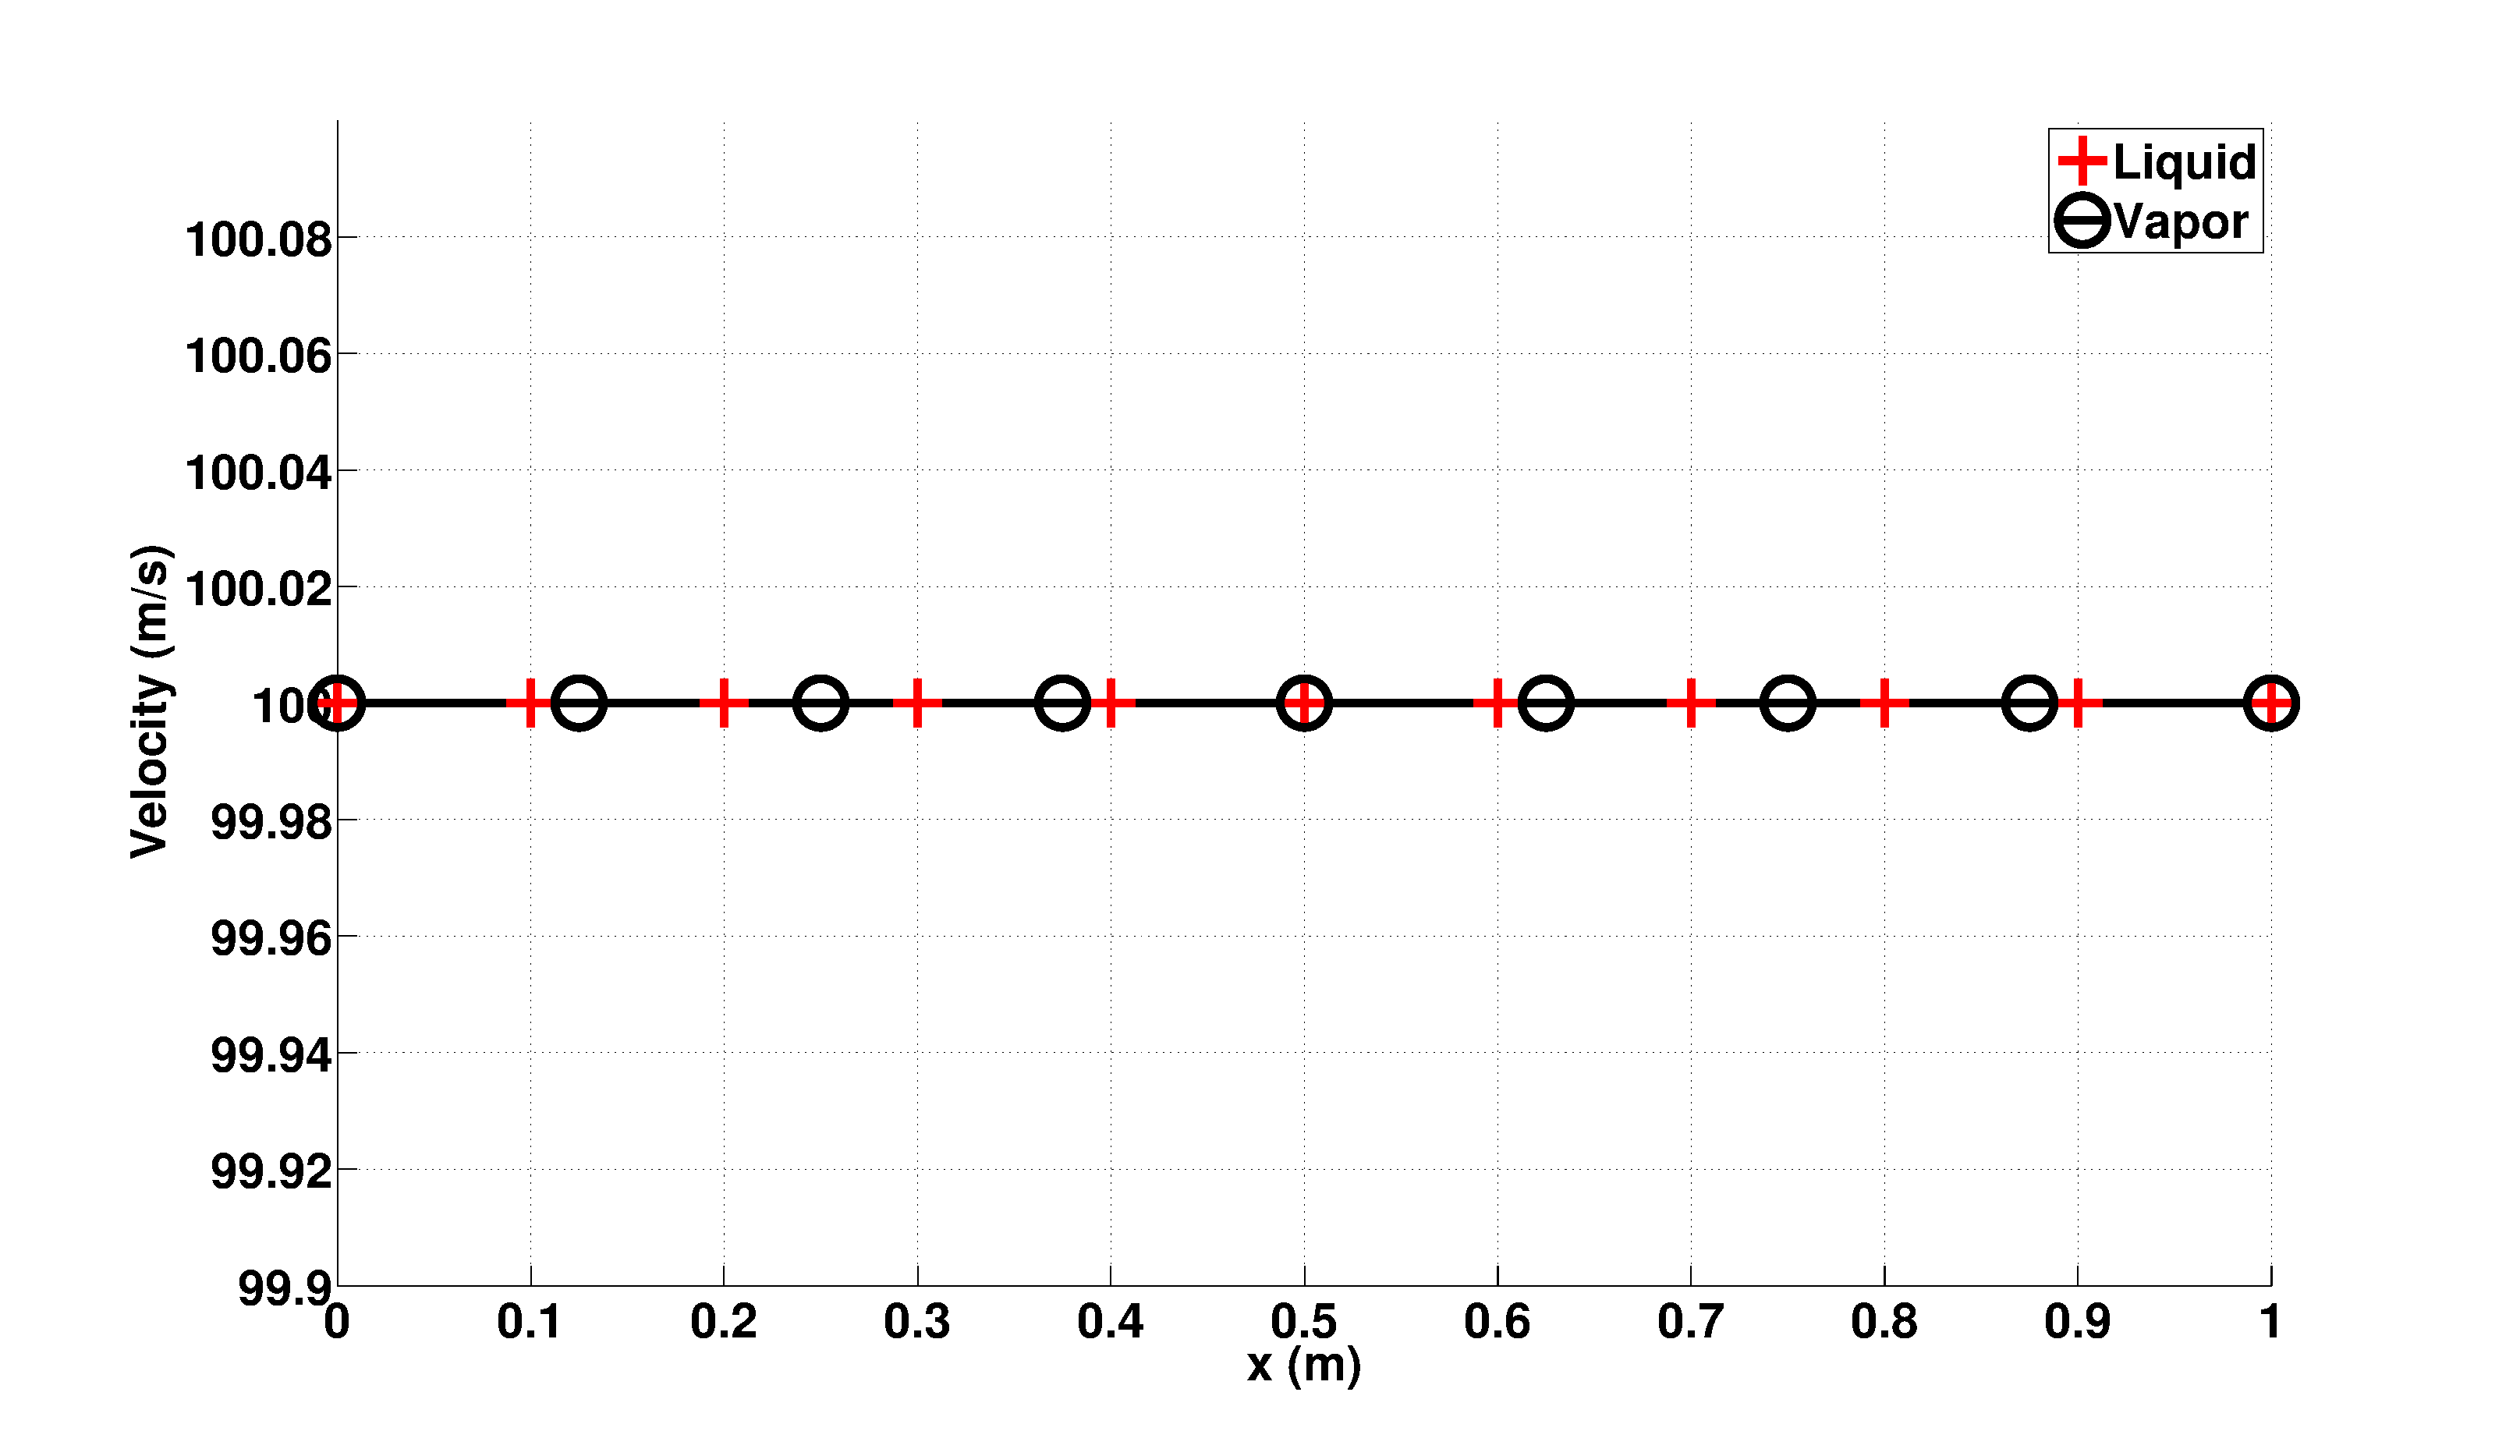
\includegraphics[width=\textwidth]{figures/vf-shock_two_phases_velocity.eps}
                \caption{Velocity}
                \label{fig:adv-vf-vel}
        \end{subfigure}%
        \begin{subfigure}[b]{0.495\textwidth}
                \centering
                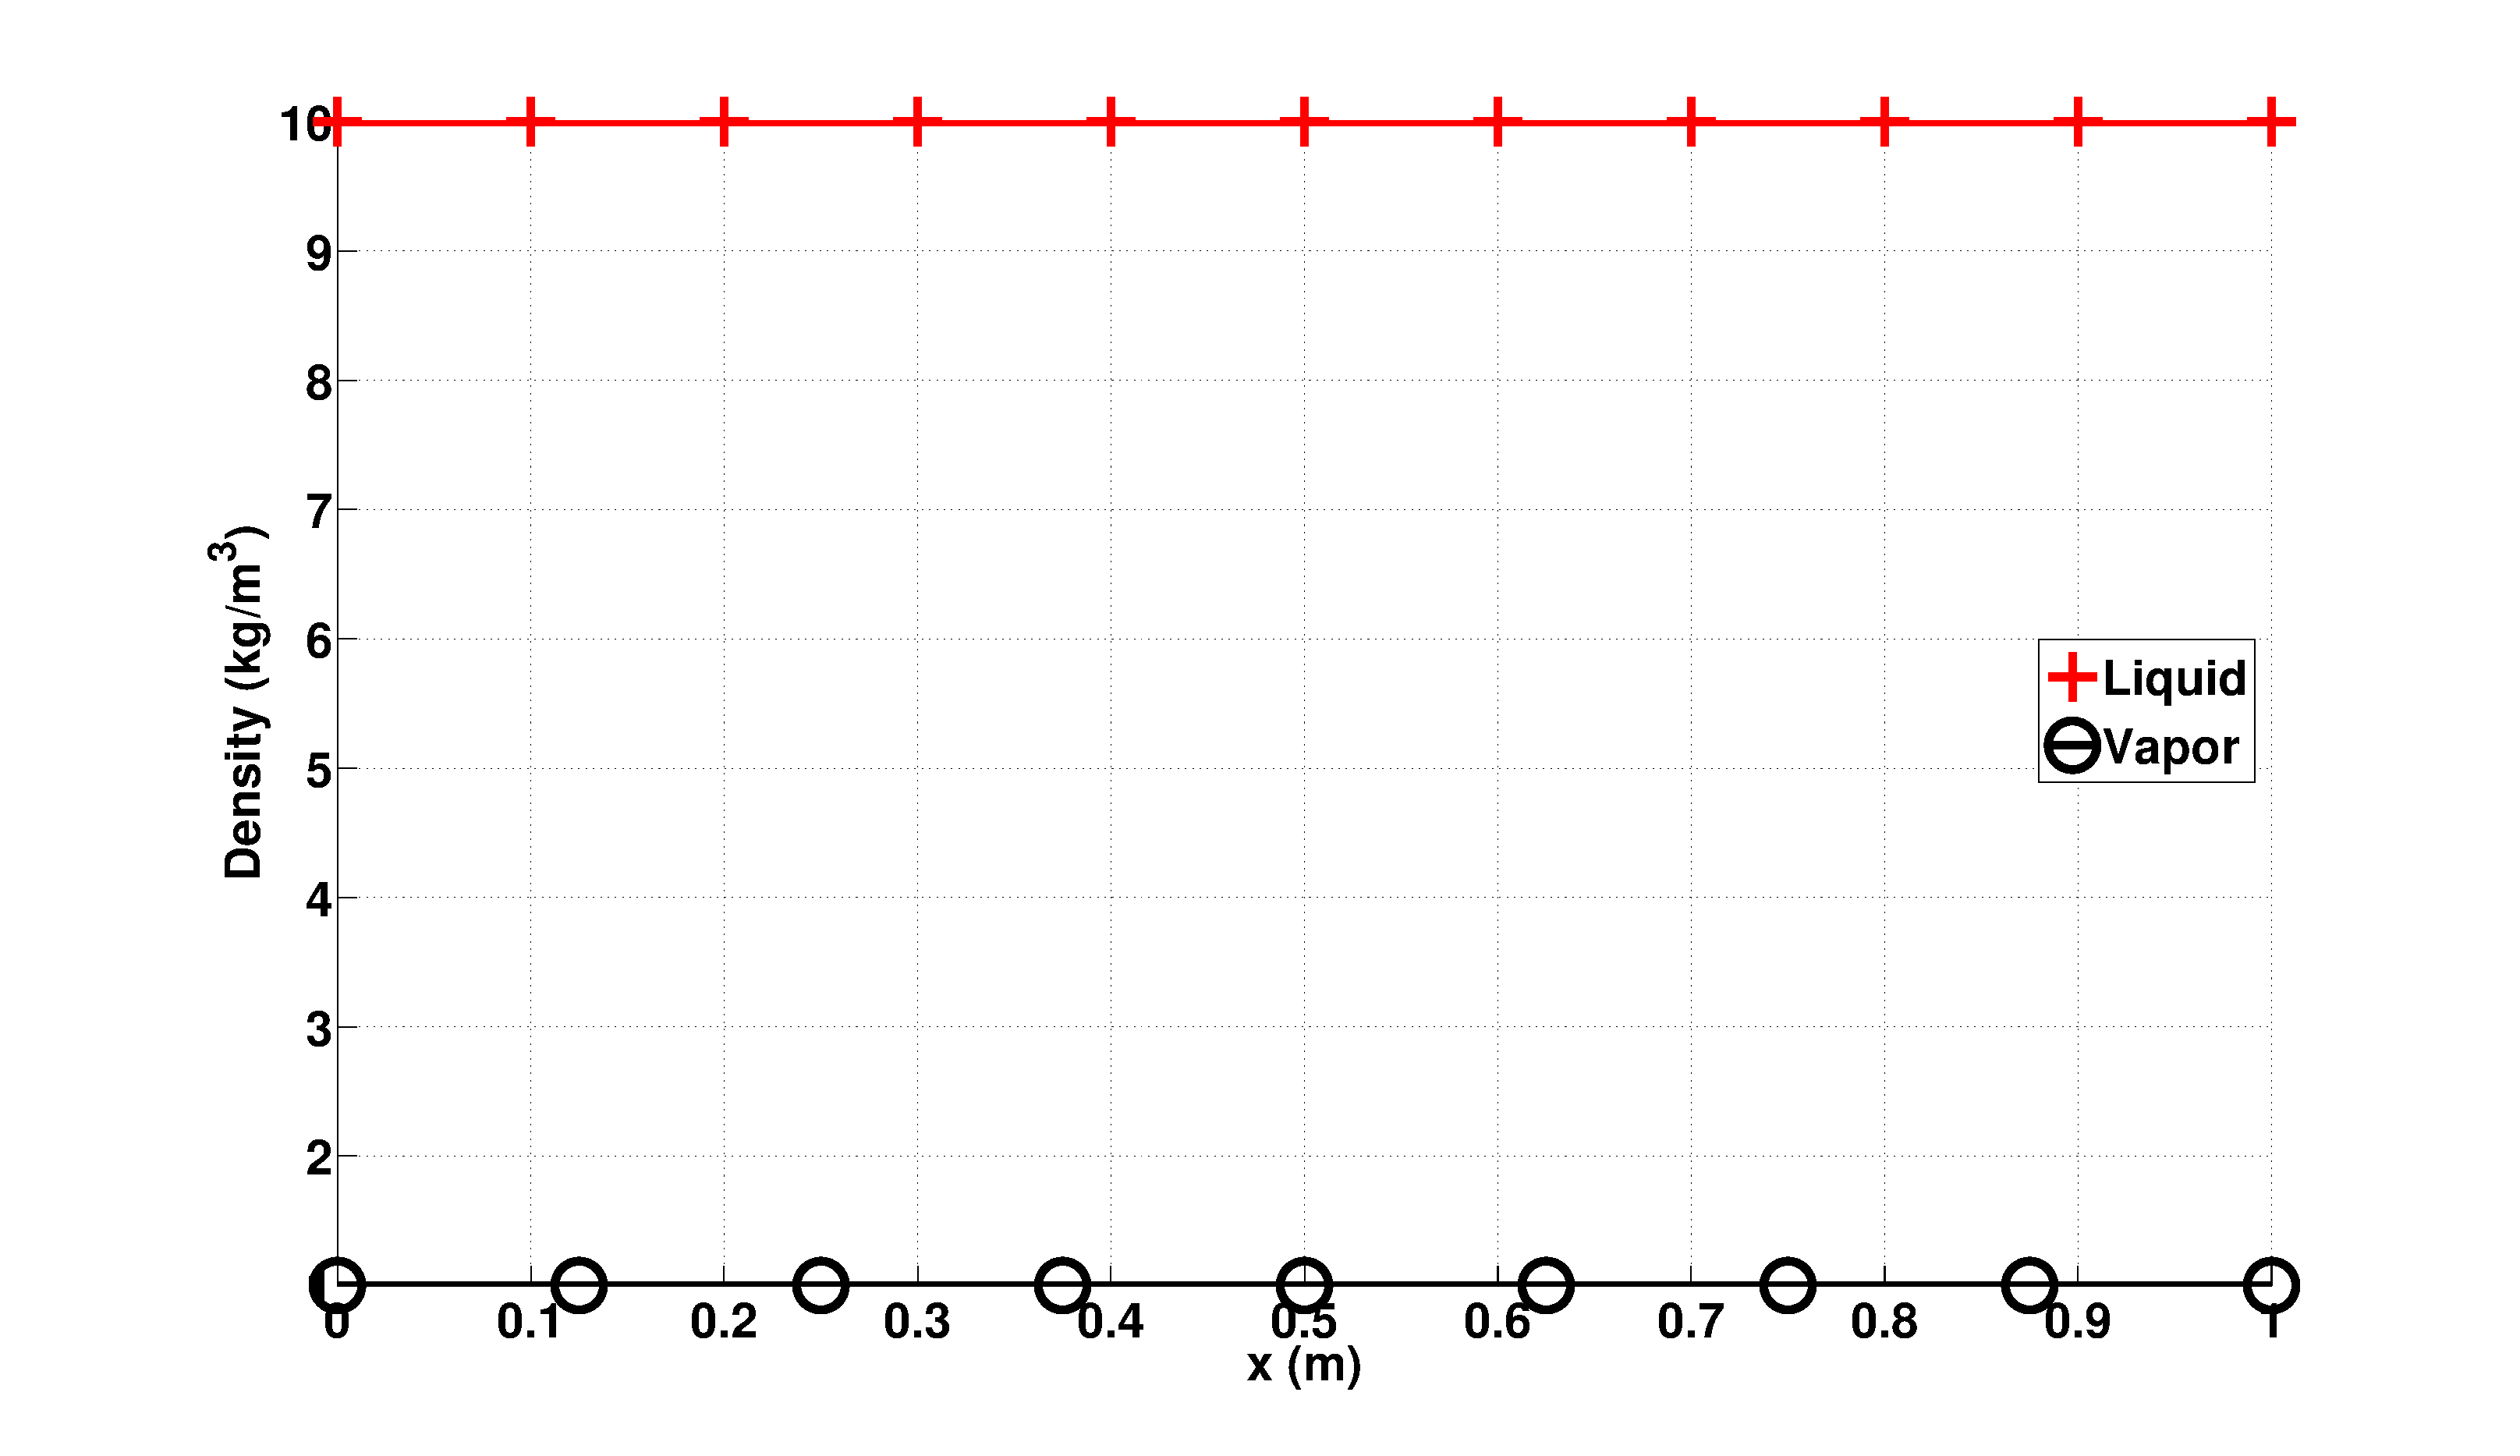
\includegraphics[width=\textwidth]{figures/vf-shock_two_phases_temperature.eps}
                \caption{Density}
                \label{fig:adv-vf-density}
        \end{subfigure}
        
        \begin{subfigure}[b]{0.495\textwidth}
                \centering
                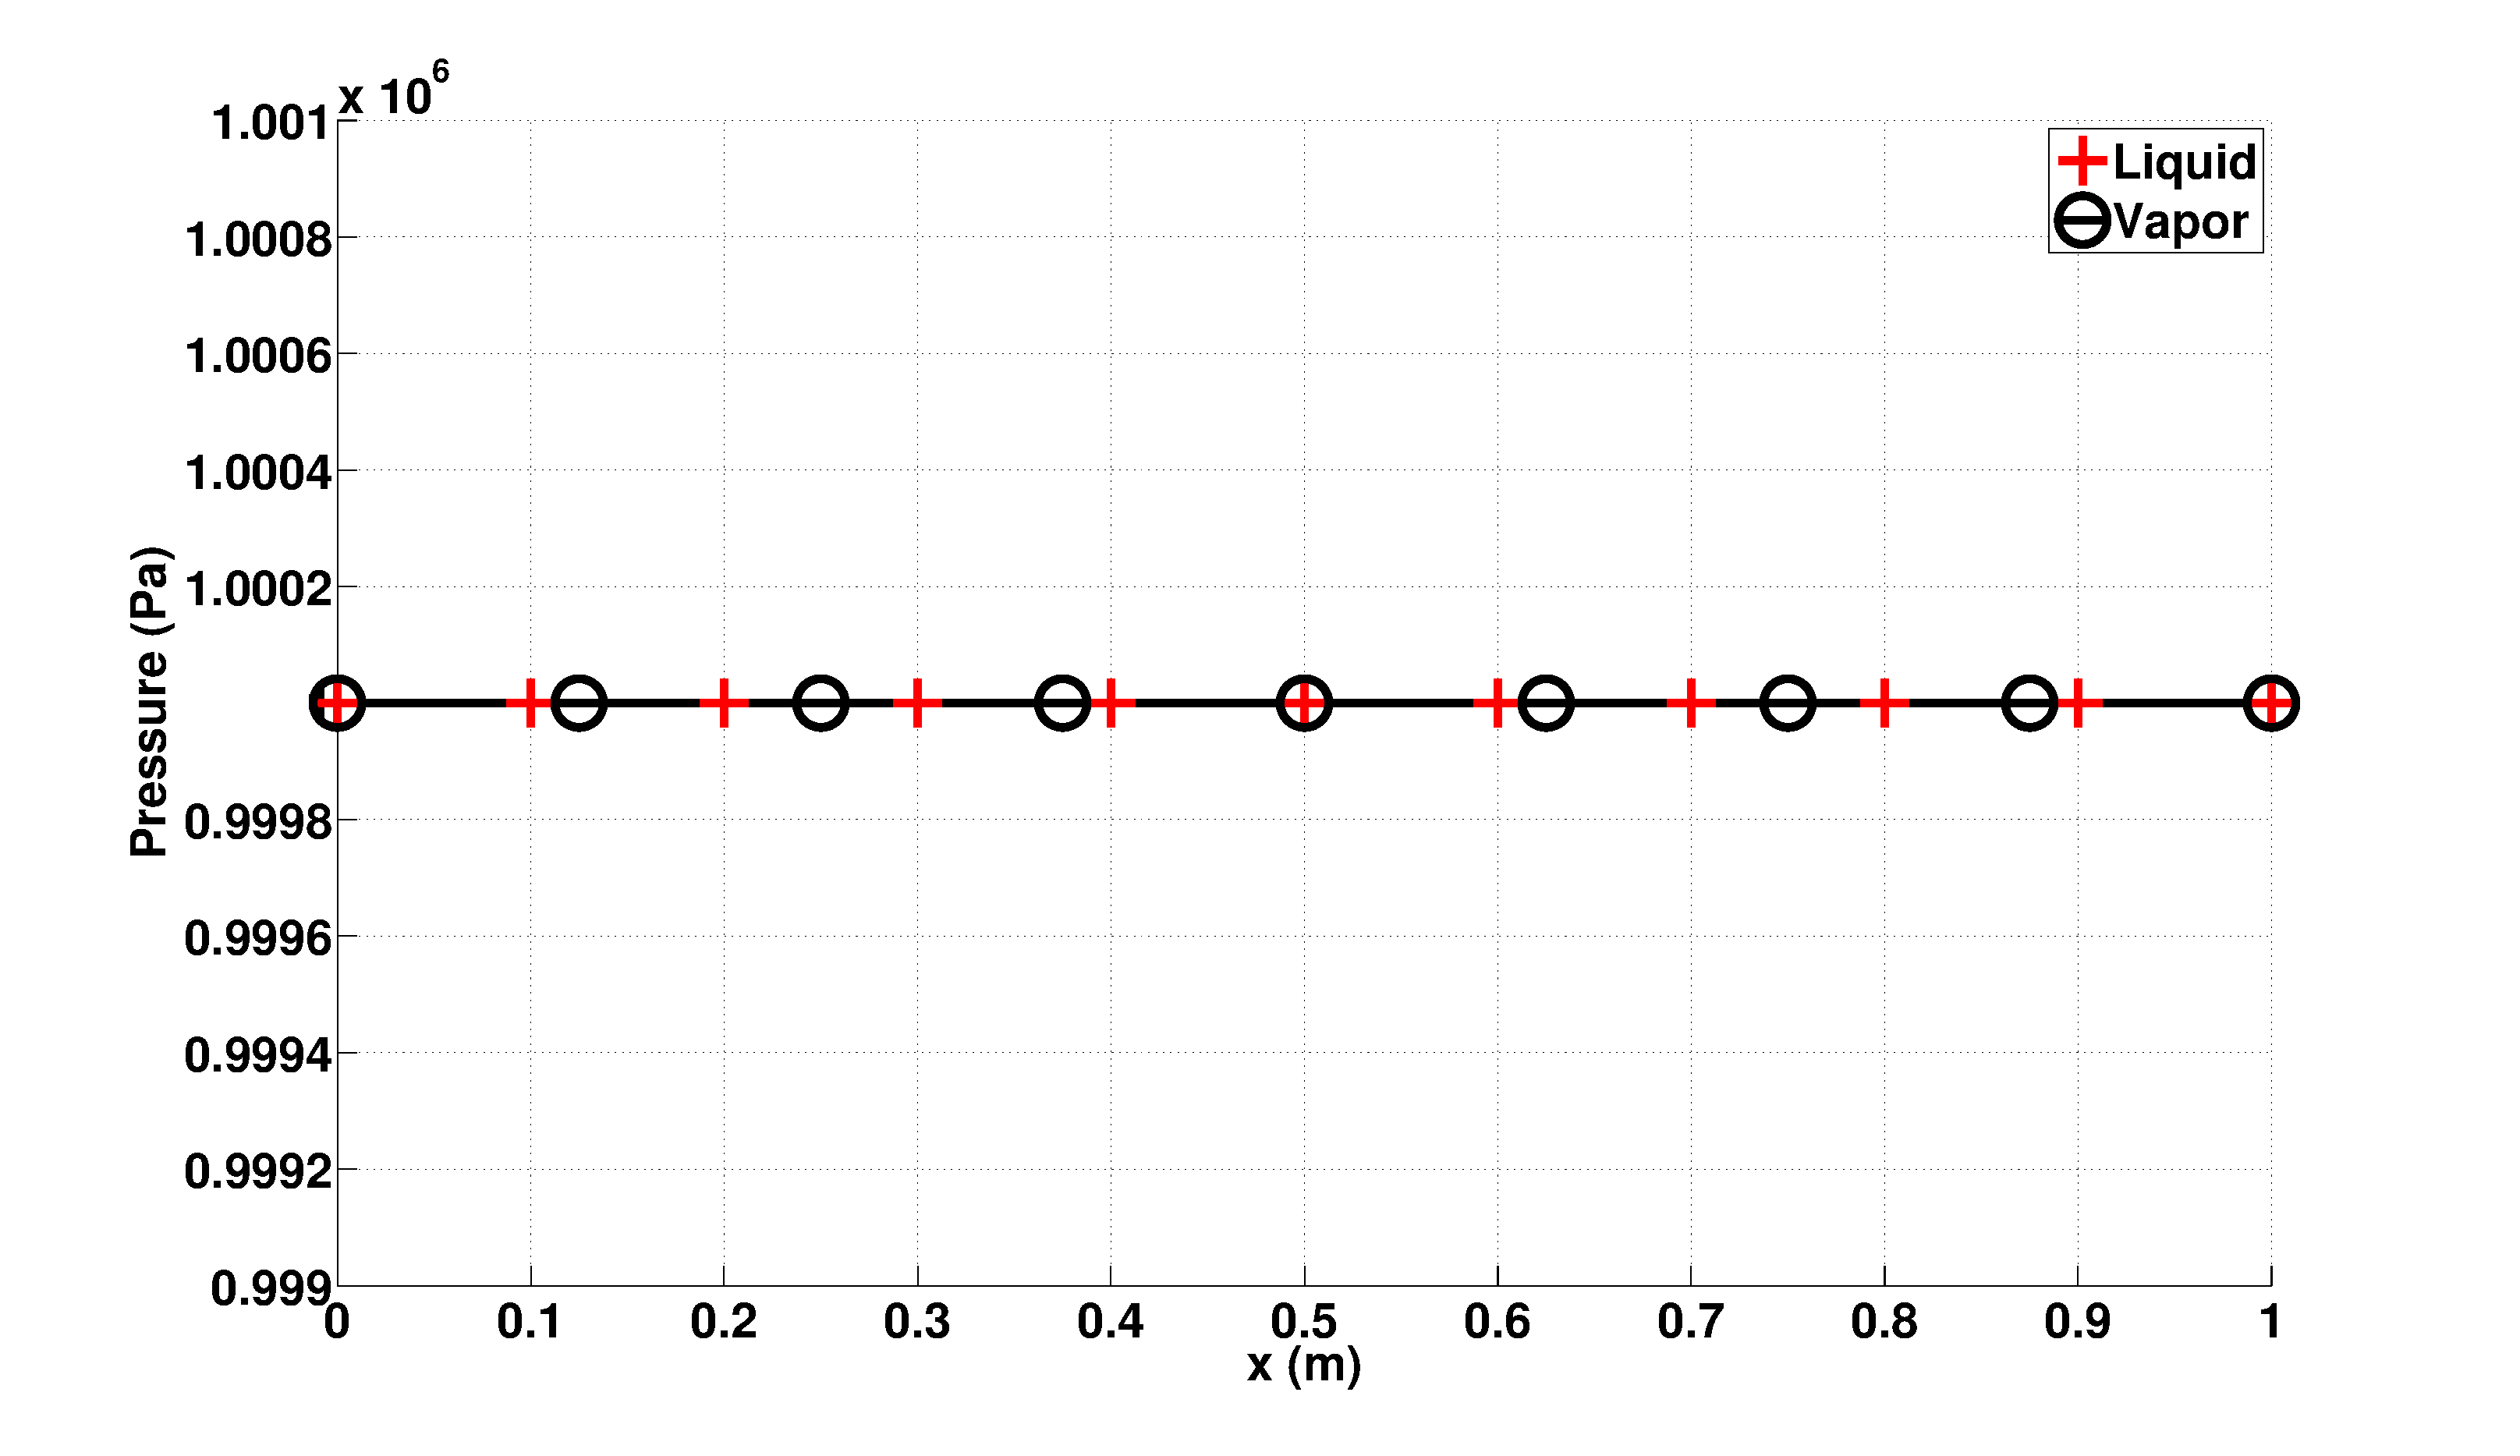
\includegraphics[width=\textwidth]{figures/vf-shock_two_phases_pressure.eps}
                \caption{Pressure}
                \label{fig:adv-vf-press}
        \end{subfigure}        
        \begin{subfigure}[b]{0.495\textwidth}
                \centering
                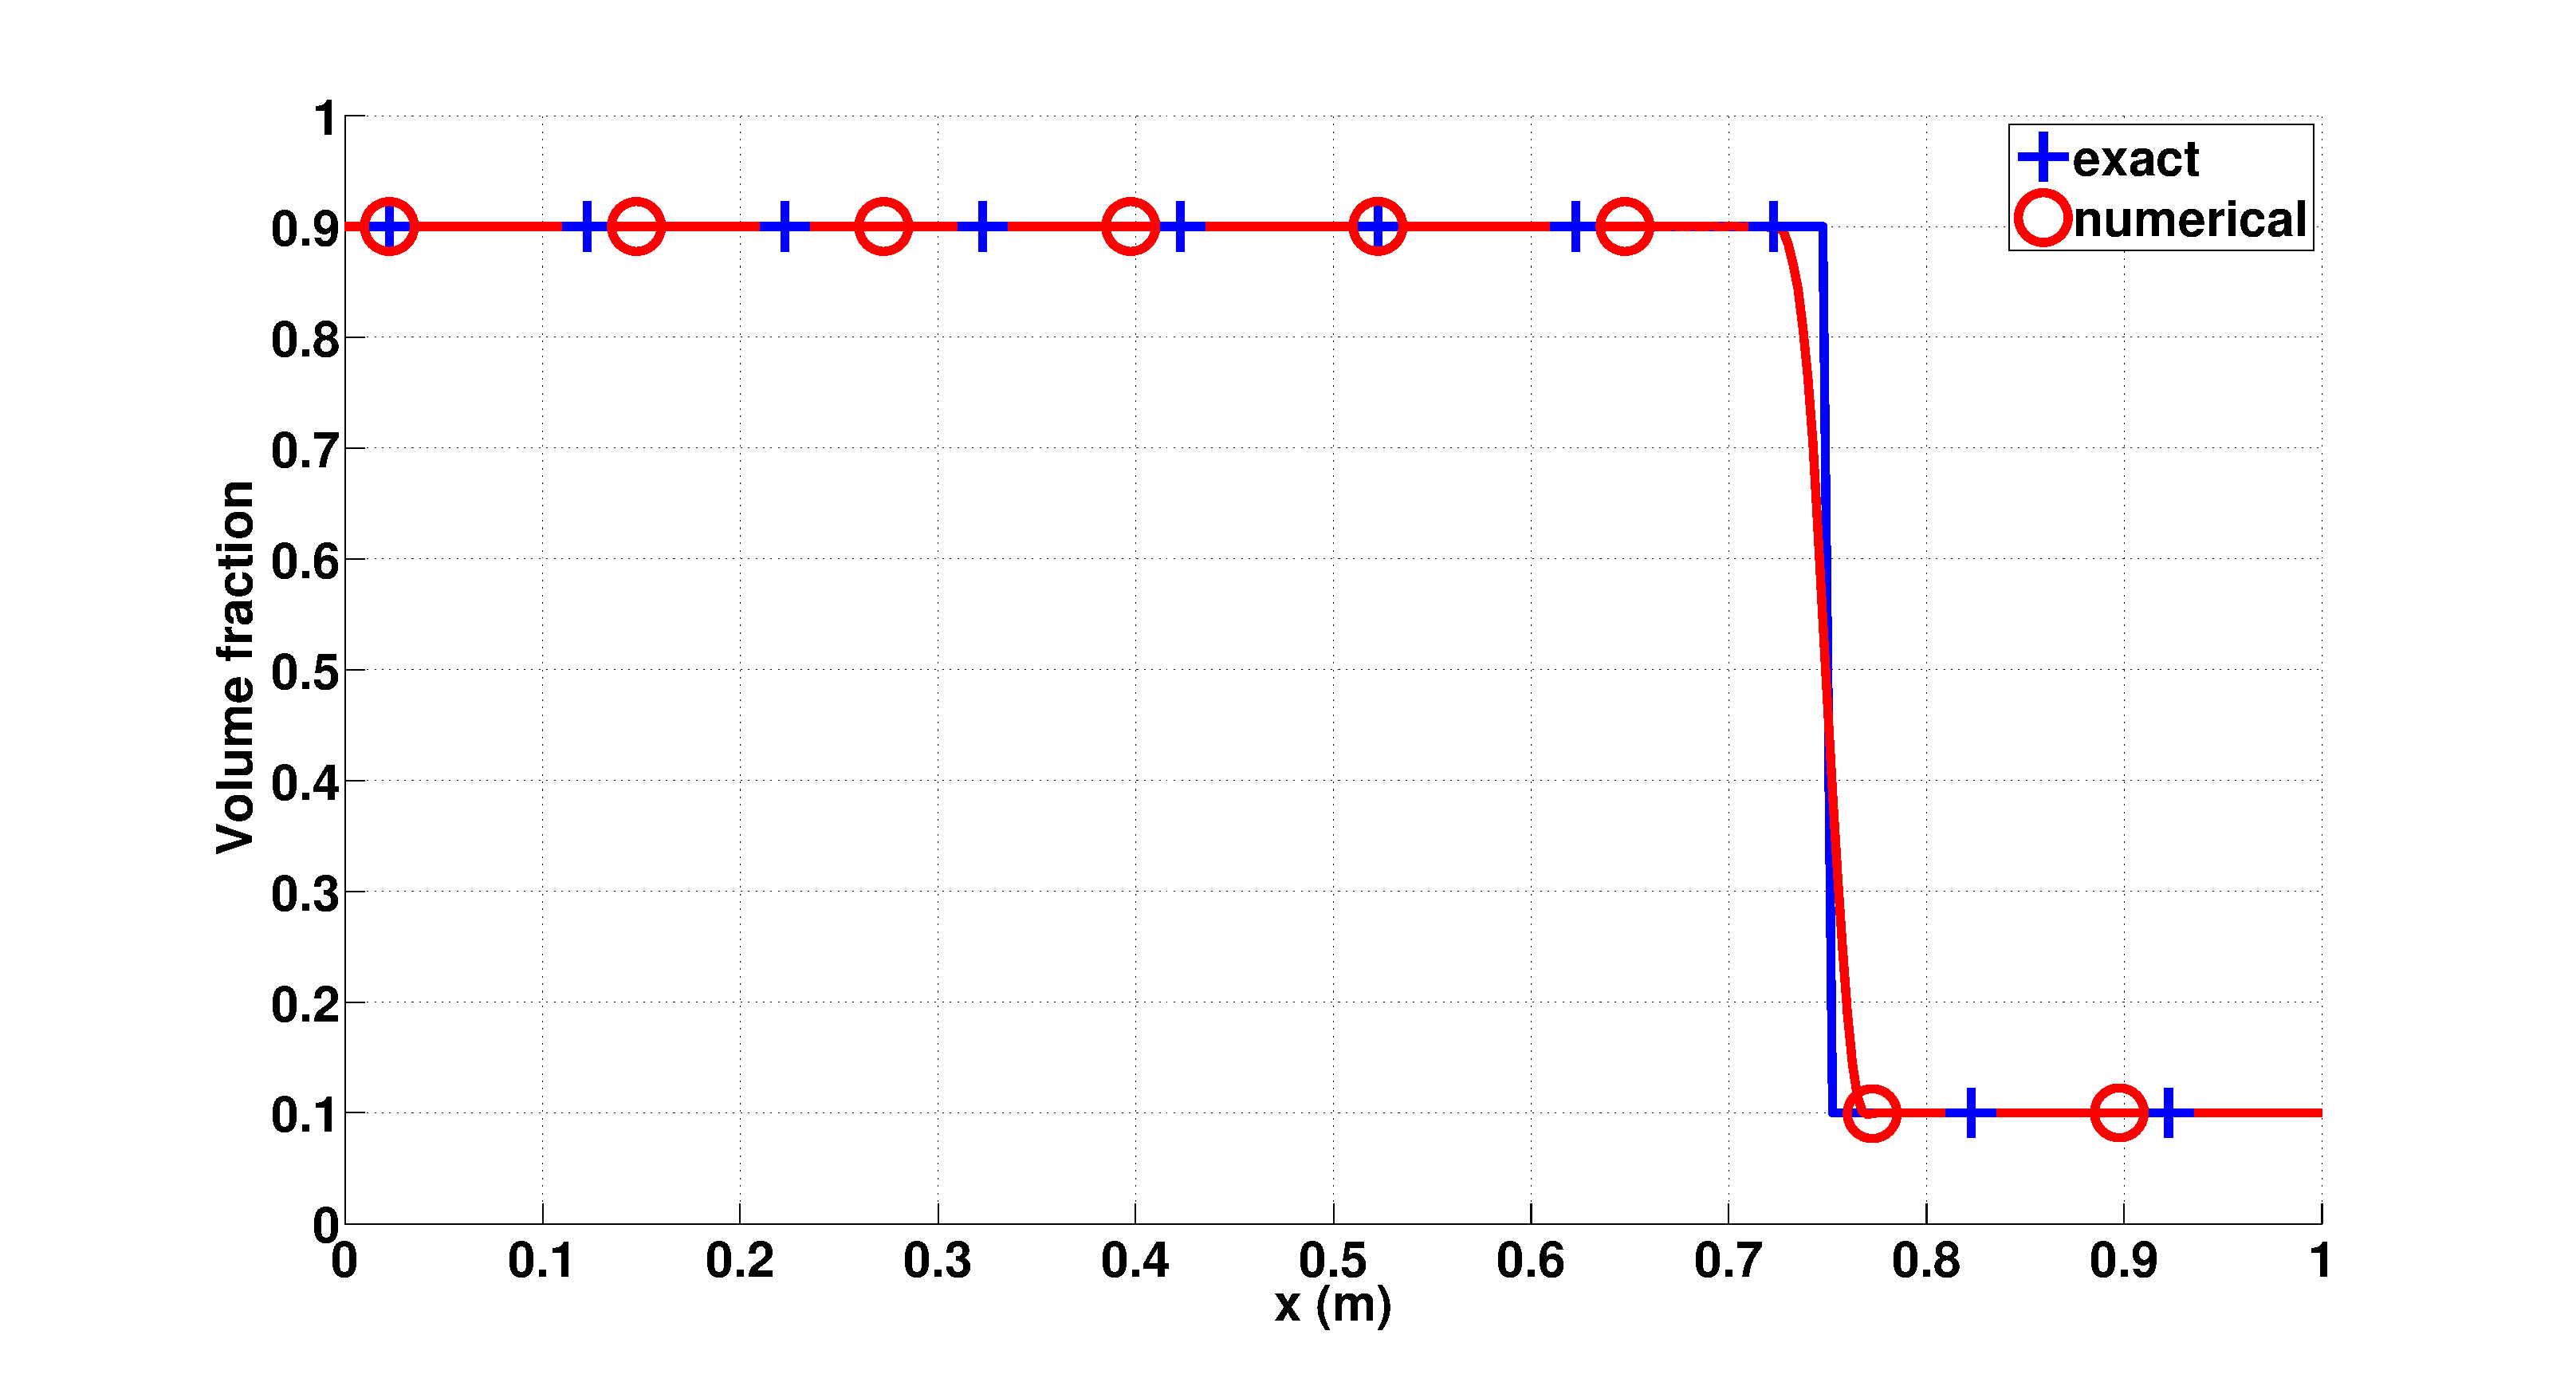
\includegraphics[width=\textwidth]{figures/advection-vol-fraction.eps}
                \caption{Volume fraction}
                \label{fig:adv-vf-vf}
        \end{subfigure}
        \caption{Numerical solution of a 1-D advection of the volume fraction at $t=1703 \ \mu s$.}\label{fig:adv-vf-variables}
\end{figure}
%
As seen in \fig{fig:adv-vf-variables}, the stabilization numerical method preserves the uniform pressure (\fig{fig:adv-vf-press}), velocity (\fig{fig:adv-vf-vel}) and density (\fig{fig:adv-vf-density}) flow conditions. The discontinuity in the volume fraction profile shown in \fig{fig:adv-vf-vf} is well resolved and does not display any oscillations.
%
\begin{figure}[H]
        \centering
        \begin{subfigure}[b]{0.495\textwidth}
                \centering
                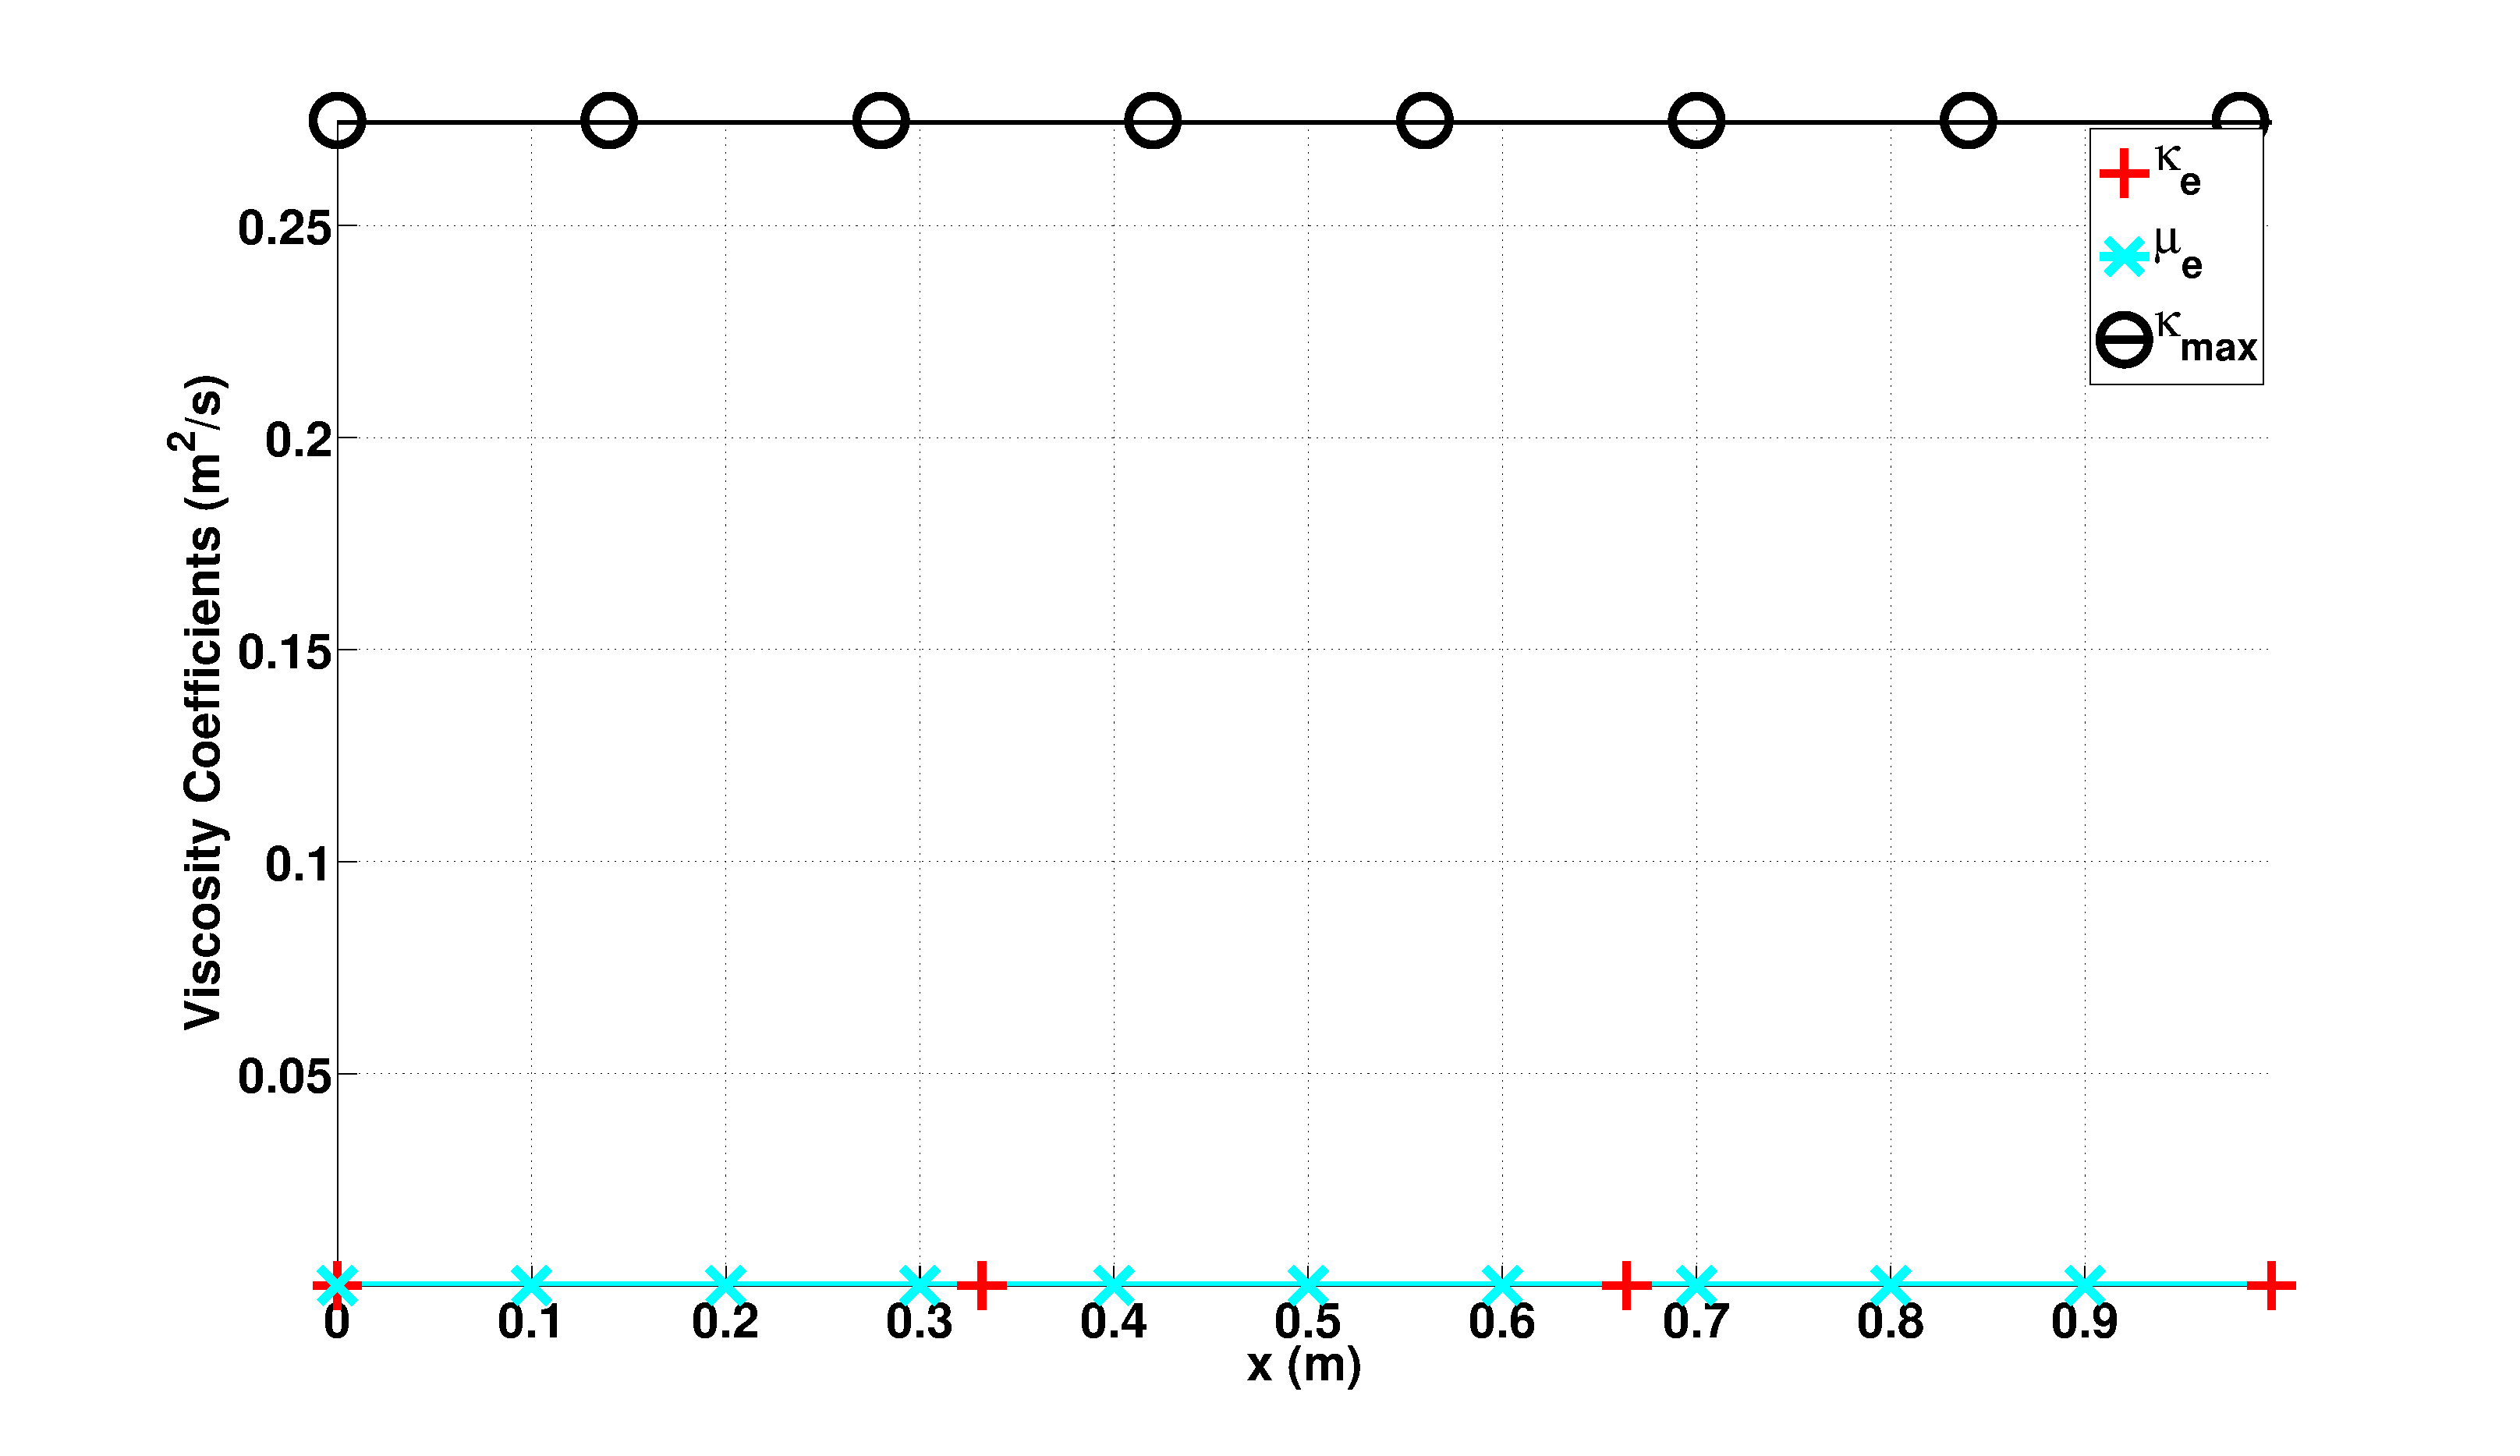
\includegraphics[width=\textwidth]{figures/liquid_viscosity.eps}
                \caption{Viscosity coefficients for phase 1.}
                \label{fig:adv-vf-1}
        \end{subfigure}%
        \begin{subfigure}[b]{0.495\textwidth}
                \centering
                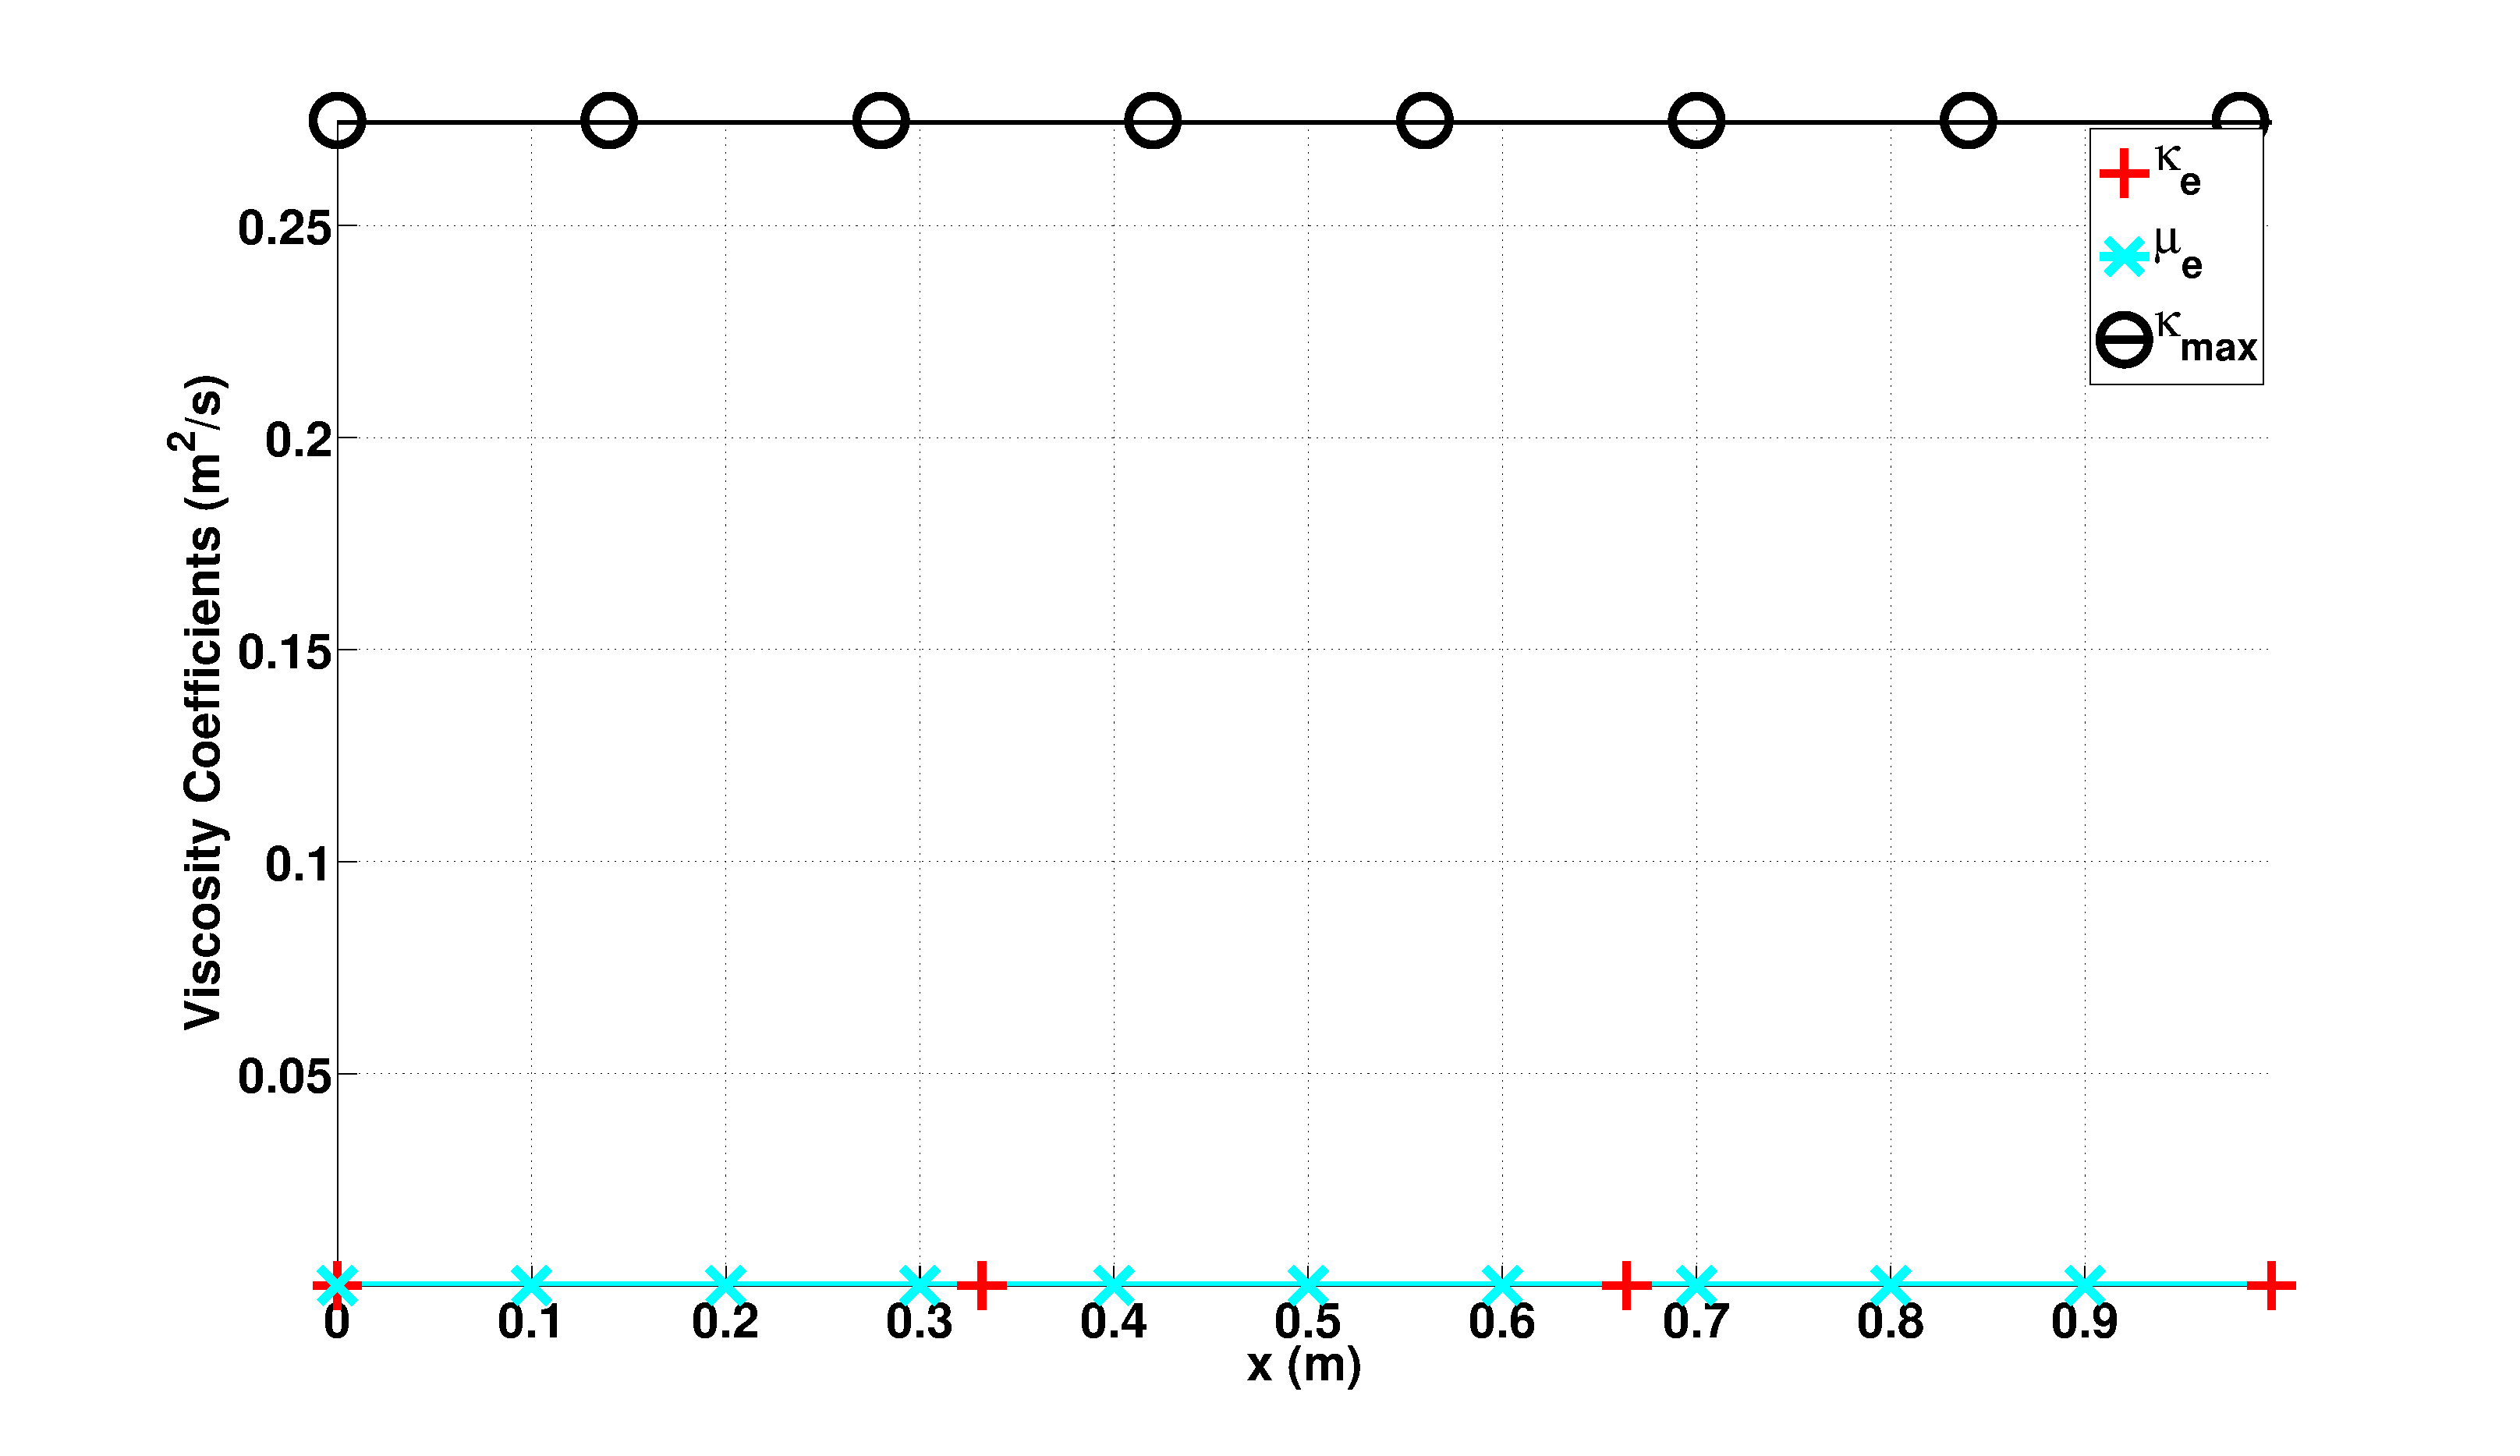
\includegraphics[width=\textwidth]{figures/liquid_viscosity.eps}
                \caption{Viscosity coefficients for phase 2}
                \label{fig:adv-vf-2}
        \end{subfigure}
        
        \begin{subfigure}[b]{0.495\textwidth}
                \centering
                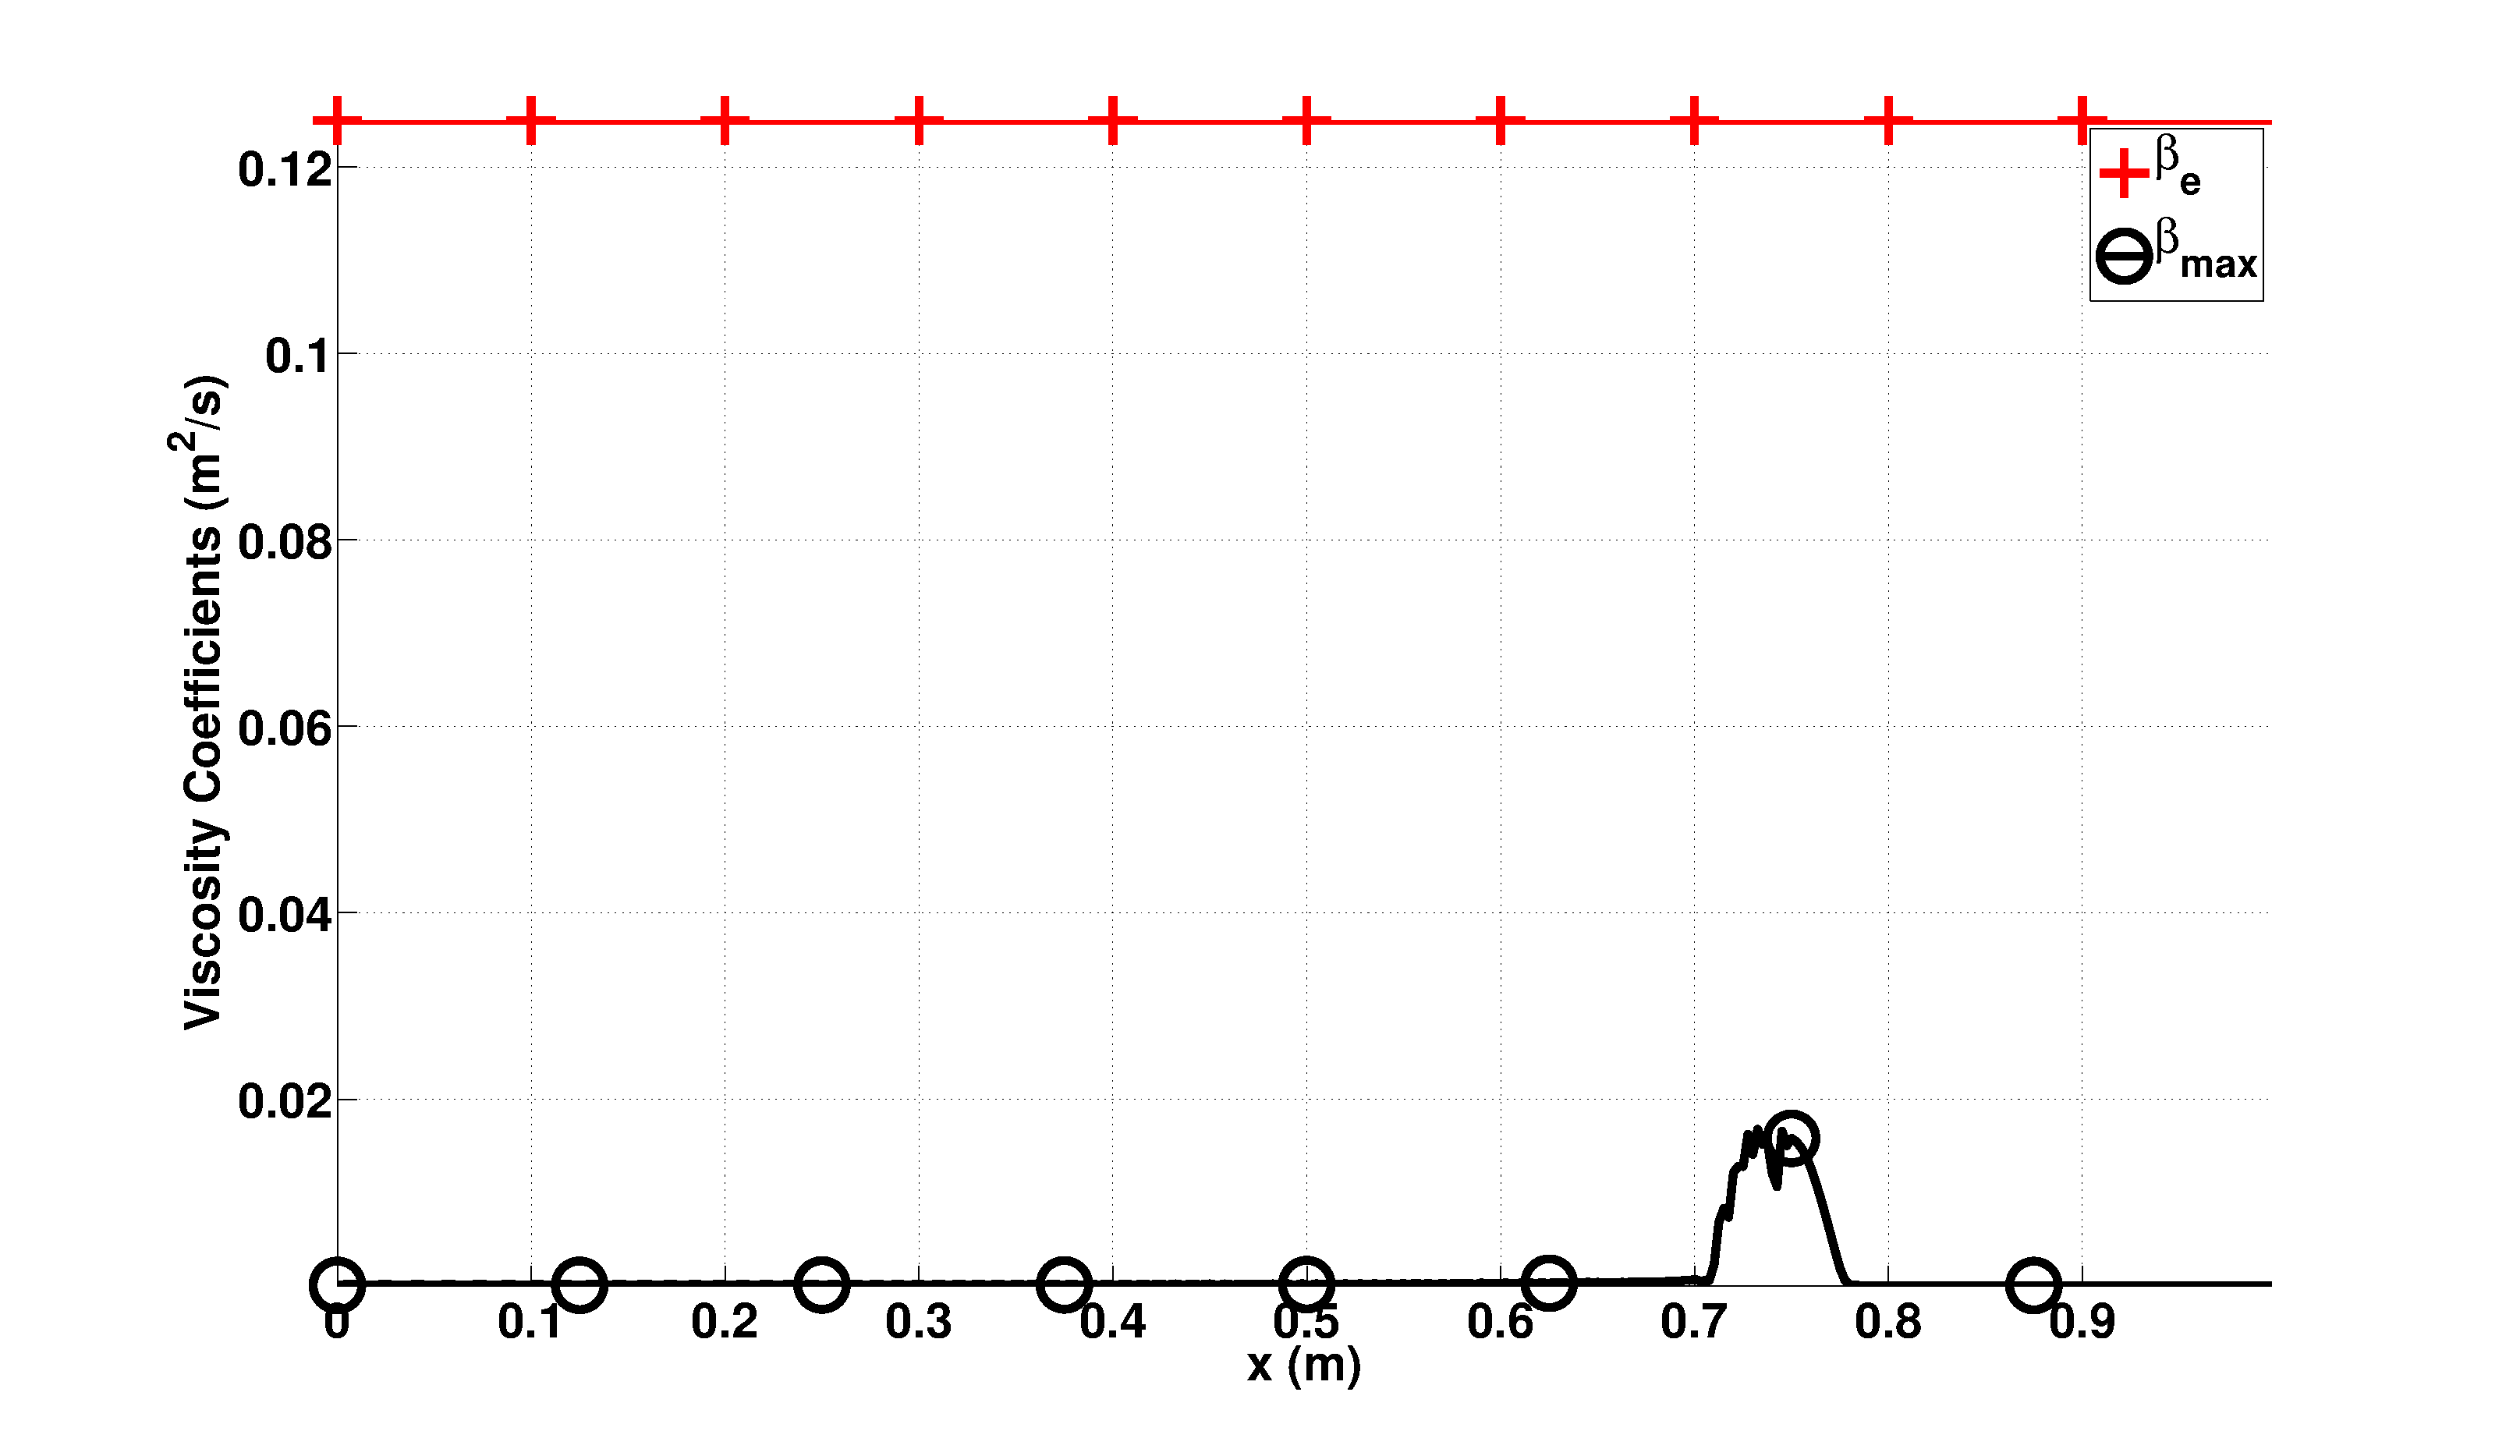
\includegraphics[width=\textwidth]{figures/liquid_beta.eps}
                \caption{Viscosity coefficients for the volume fraction equation of phase 1.}
                \label{fig:adv-vf-beta}
        \end{subfigure}        
        \caption{Viscosity coefficients profiles for a 1-D advection of the volume fraction at $t=1703 \ \mu s$.}\label{adv-vf-visc}
\end{figure}
%
The phasic viscosity coefficients $\mu_k$ and $\kappa_k$ are equal to zero for both phases as shown in \fig{fig:adv-vf-1} and \fig{fig:adv-vf-2}, since the phasic flow conditions (pressure, density and velocity) are uniform. However, the viscosity coefficient $\beta_k$ is peaked in the discontinuity region as expected (\fig{fig:adv-vf-beta}). This test clearly shows that the stabilization method does not induce any artificial waves in the pressure, velocity and density profiles due to the smearing of the discontinuity in the volume fraction profile. 

We also performed a convergence study by computing the L$_1$ and L$_2$ norms of the error between the numerical and the exact solutions for the volume fraction variable only. The exact solution was obtained from a Riemann solver. Following REFS, the convergence rate for the L$_1$ and L$_2$ norms are known to be $\frac{p+0.5}{p+1}$ and $0.5\frac{p+0.5}{p+1}$, respectively, where $p$ is the polynomial order of the test function used. Because we are using linear polynomial test functions, $p=1$, the corresponding theoretical convergence rates for the L$_1$ and L$_2$ norms are $0.75$ and $0.37$, respectively. 
%
\begin{table}[H]
\begin{center}
 \caption{\label{tbl:conv_rate_norm} L$_1$ and L$_2$ norms of the error for the liquid volume fraction.}
 \begin{tabular}{|c|c|c|c|c|}
 \hline
cells  & $L1$ norm  & $L1$ rate   & $L2$ norm & $L2$ rate  \\ \hline
25     & 5.3721017 $10^{-2}$ & $-$    & 1.0624715 $10^{-1}$ & \\ \hline
50     & 3.4607761 $10^{-2}$ & 0.634 & 8.7183697 $10^{-2}$  & 0.285 \\ \hline
100   & 2.1396498 $10^{-2}$ & 0.694 & 6.6006650 $10^{-2}$  & 0.401 \\ \hline
200   & 1.2915332 $10^{-2}$ & 0.728 & 5.2105365 $10^{-2}$  & 0.341 \\ \hline
400   & 7.6834125 $10^{-3}$ & 0.749 & 4.0365699 $10^{-2}$  & 0.368 \\ \hline
800   & 4.5825174 $10^{-3}$ & 0.745 & 3.1465921 $10^{-2}$  & 0.359 \\ \hline
1600 & 2.7153206 $10^{-3}$ & 0.755 & 2.4413174 $10^{-2}$ & 0.366 \\ \hline
\end{tabular}
\end{center}
\end{table}
%
The theoretical convergence rates match the convergence rates computed from the numerical solutions as shown in \tbl{tbl:conv_rate_norm}, which proves correct behavior of the EVM n this particular test.
%
%%%%%%%%%%%%%%%%%%%%%%%%%%%%%%%%%%%%%
\subsubsection{Shock tube with two independent fluids}\label{sec:shock-tube-two-indep-fluids}
%%%%%%%%%%%%%%%%%%%%%%%%%%%%%%%%%%%%%
%
We now consider a 1-D straight pipe of length L $=1$ $m$ filled with the same fluids as in \sct{sec:vf-advection-test}. The objective of this test is to show that 
the viscous regularization can efficiently stabilize two independent fluids without creating artificial waves in the volume fraction solution that should remain 
constant (this test is complementary of the previous test presented in \sct{sec:vf-advection-test}). A membrane located at $x=0.5 \ m$, separates the pipe in two chambers with a high pressure ($P_{left} = 1$ $MPa$) on the left side and a low pressure ($P_{left} = 0.1$ 
$MPa$) in the right side. Both fluids are initially at rest. The volume fraction is set to $0.5$ which means each side of the chamber contains a mixture of two 
fluids. Dirichlet boundary conditions are used. Since the velocity and pressure relaxation coefficients $\mu_P$ and $\lambda_u$ are set to zero, the two 
fluids will behave independently to each other and the volume fraction is expected to remain uniform during the simulation. An exact solution is available for 
each fluid which simply corresponds to the single-phase exact solution obtained from a Riemann solver. Note that the same numerical results could be obtained by solving the $1$-D Euler equations for each phase. The geometry is discretized with an uniform mesh of 
500 cells and run with a CFL of one until the final time $t = 305$ $\mu s$. The numerical solutions of the density, velocity, pressure and volume fraction are given in \fig{fig:indp-phase-variables}. Profiles of the phasic viscosity coefficients $\mu_k$, $\kappa_k$ and $\beta_k$ are given in \fig{fig:indp-phase-visc-coeff}.
%
\begin{figure}[H]
        \centering
        \begin{subfigure}[b]{0.495\textwidth}
                \centering
                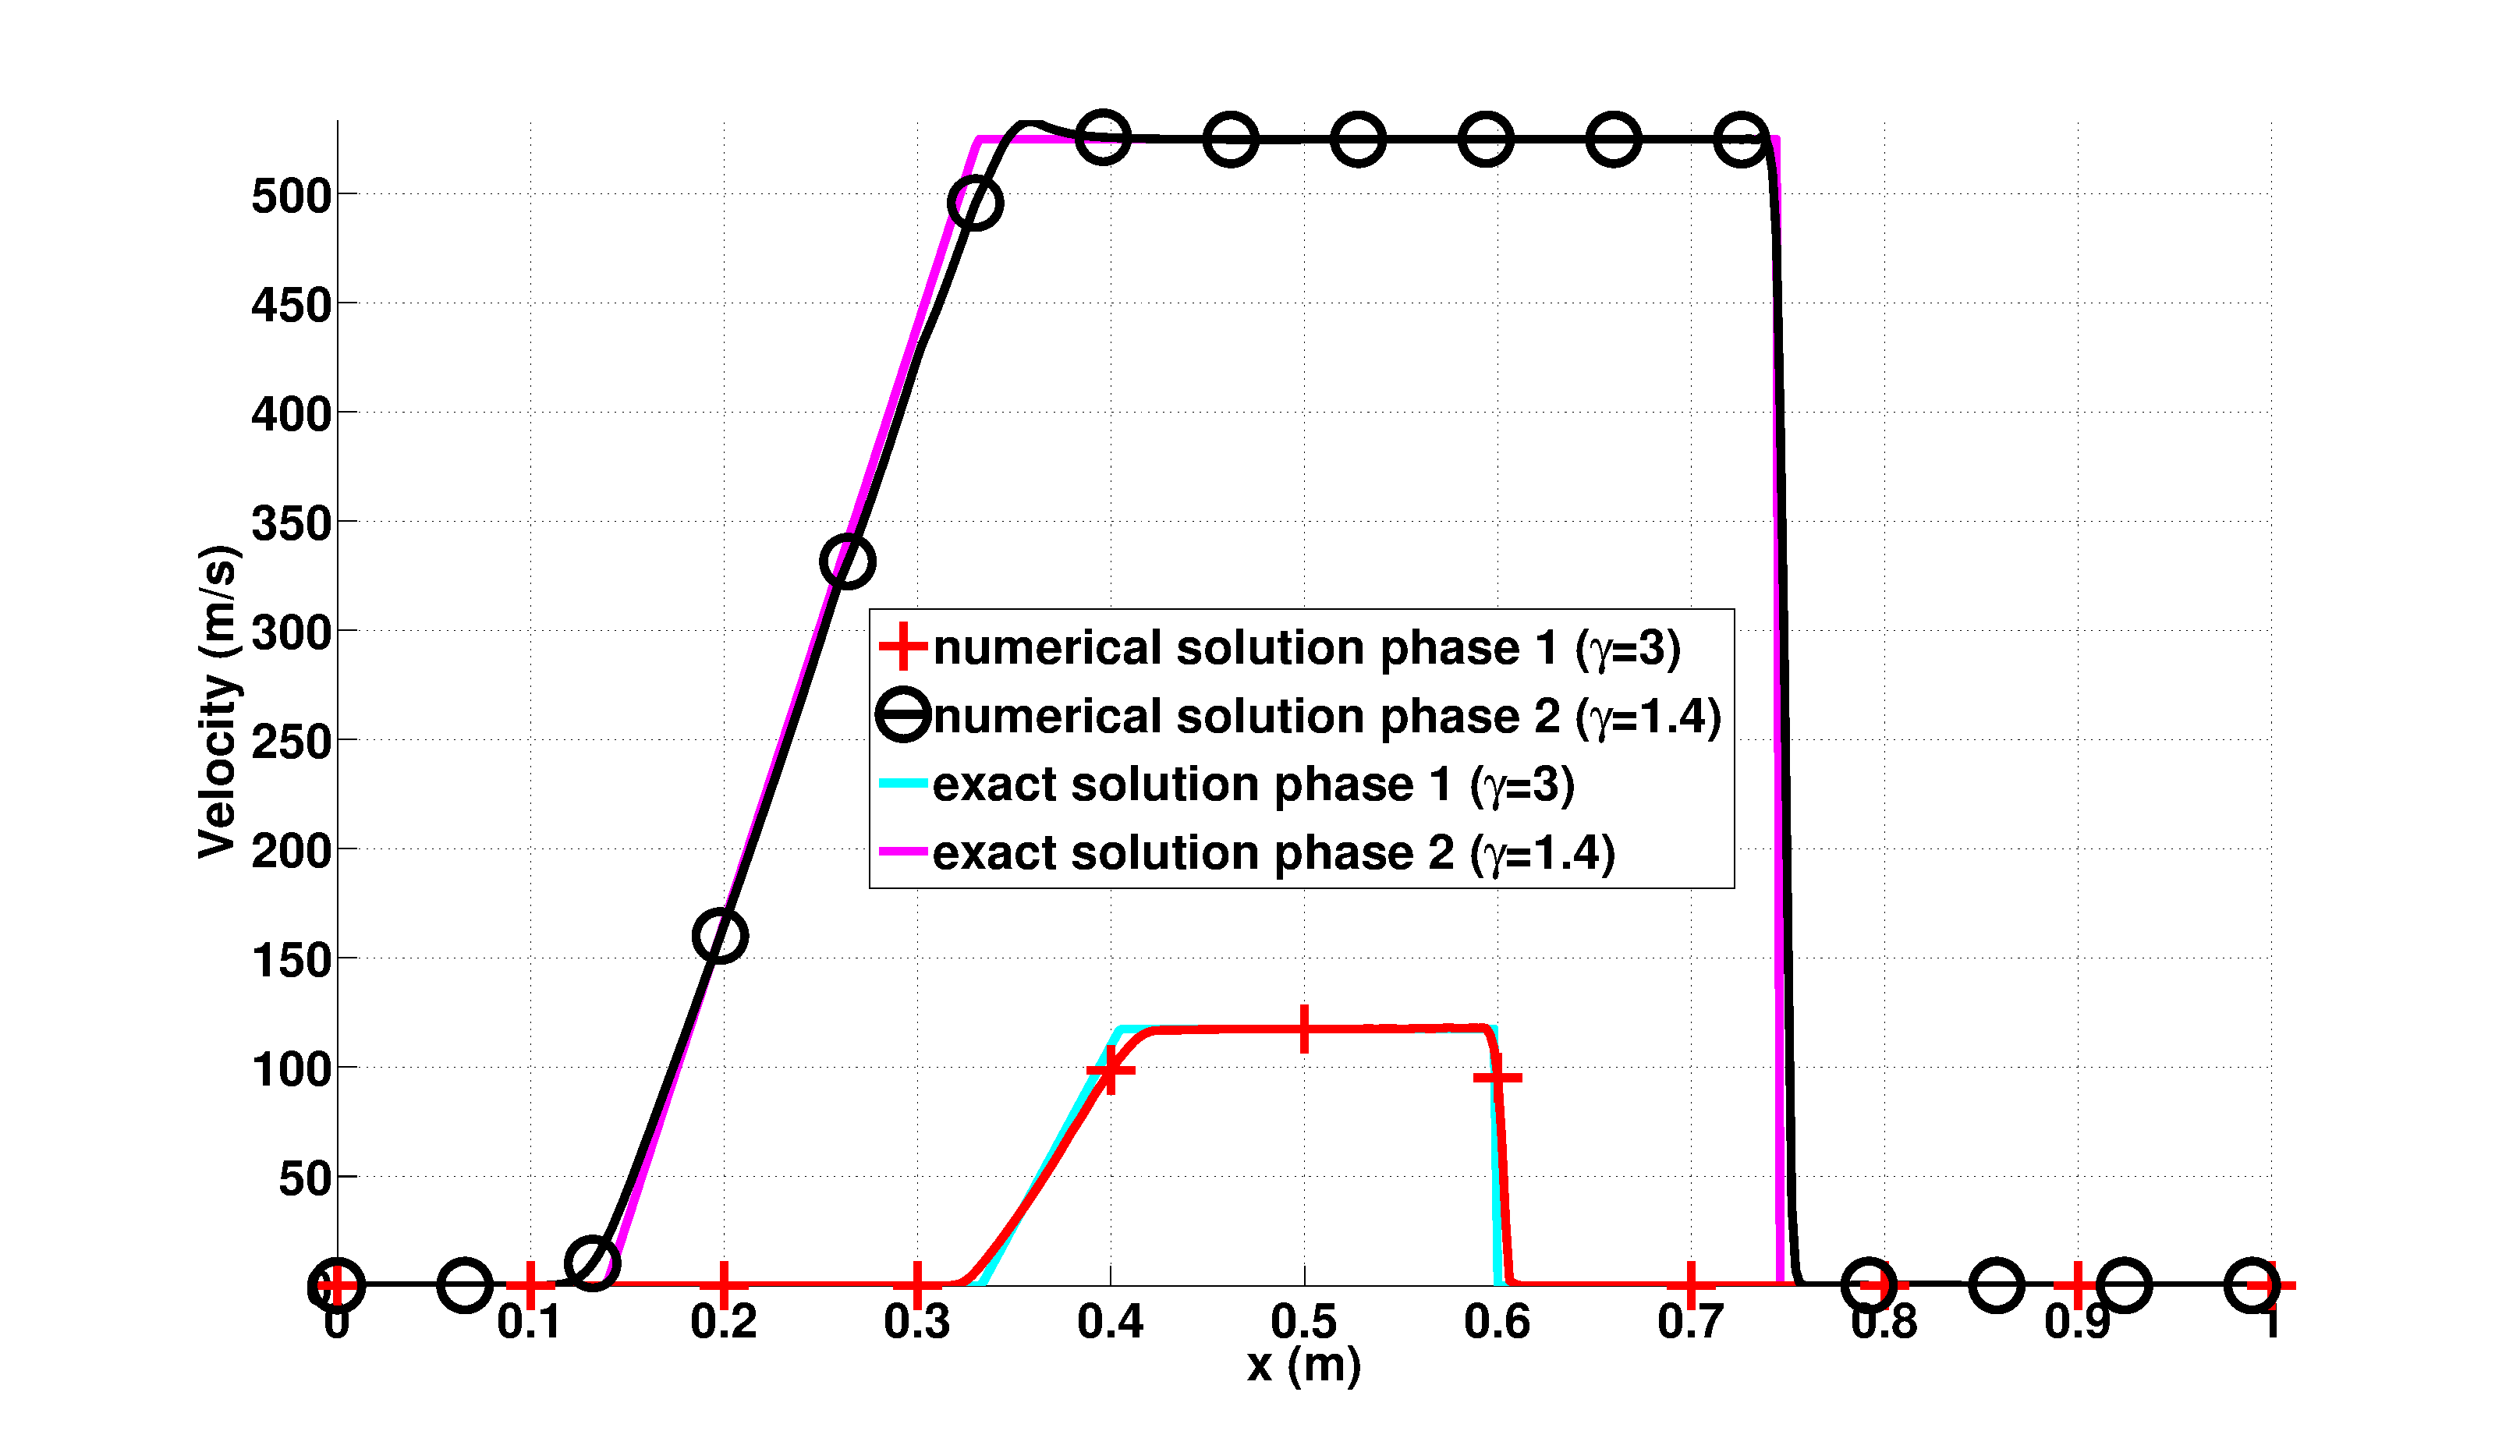
\includegraphics[width=\textwidth]{figures/two_phases_velocity.eps}
                \caption{Velocity}
                \label{fig:indp-phase-vel}
        \end{subfigure}%
        \begin{subfigure}[b]{0.495\textwidth}
                \centering
                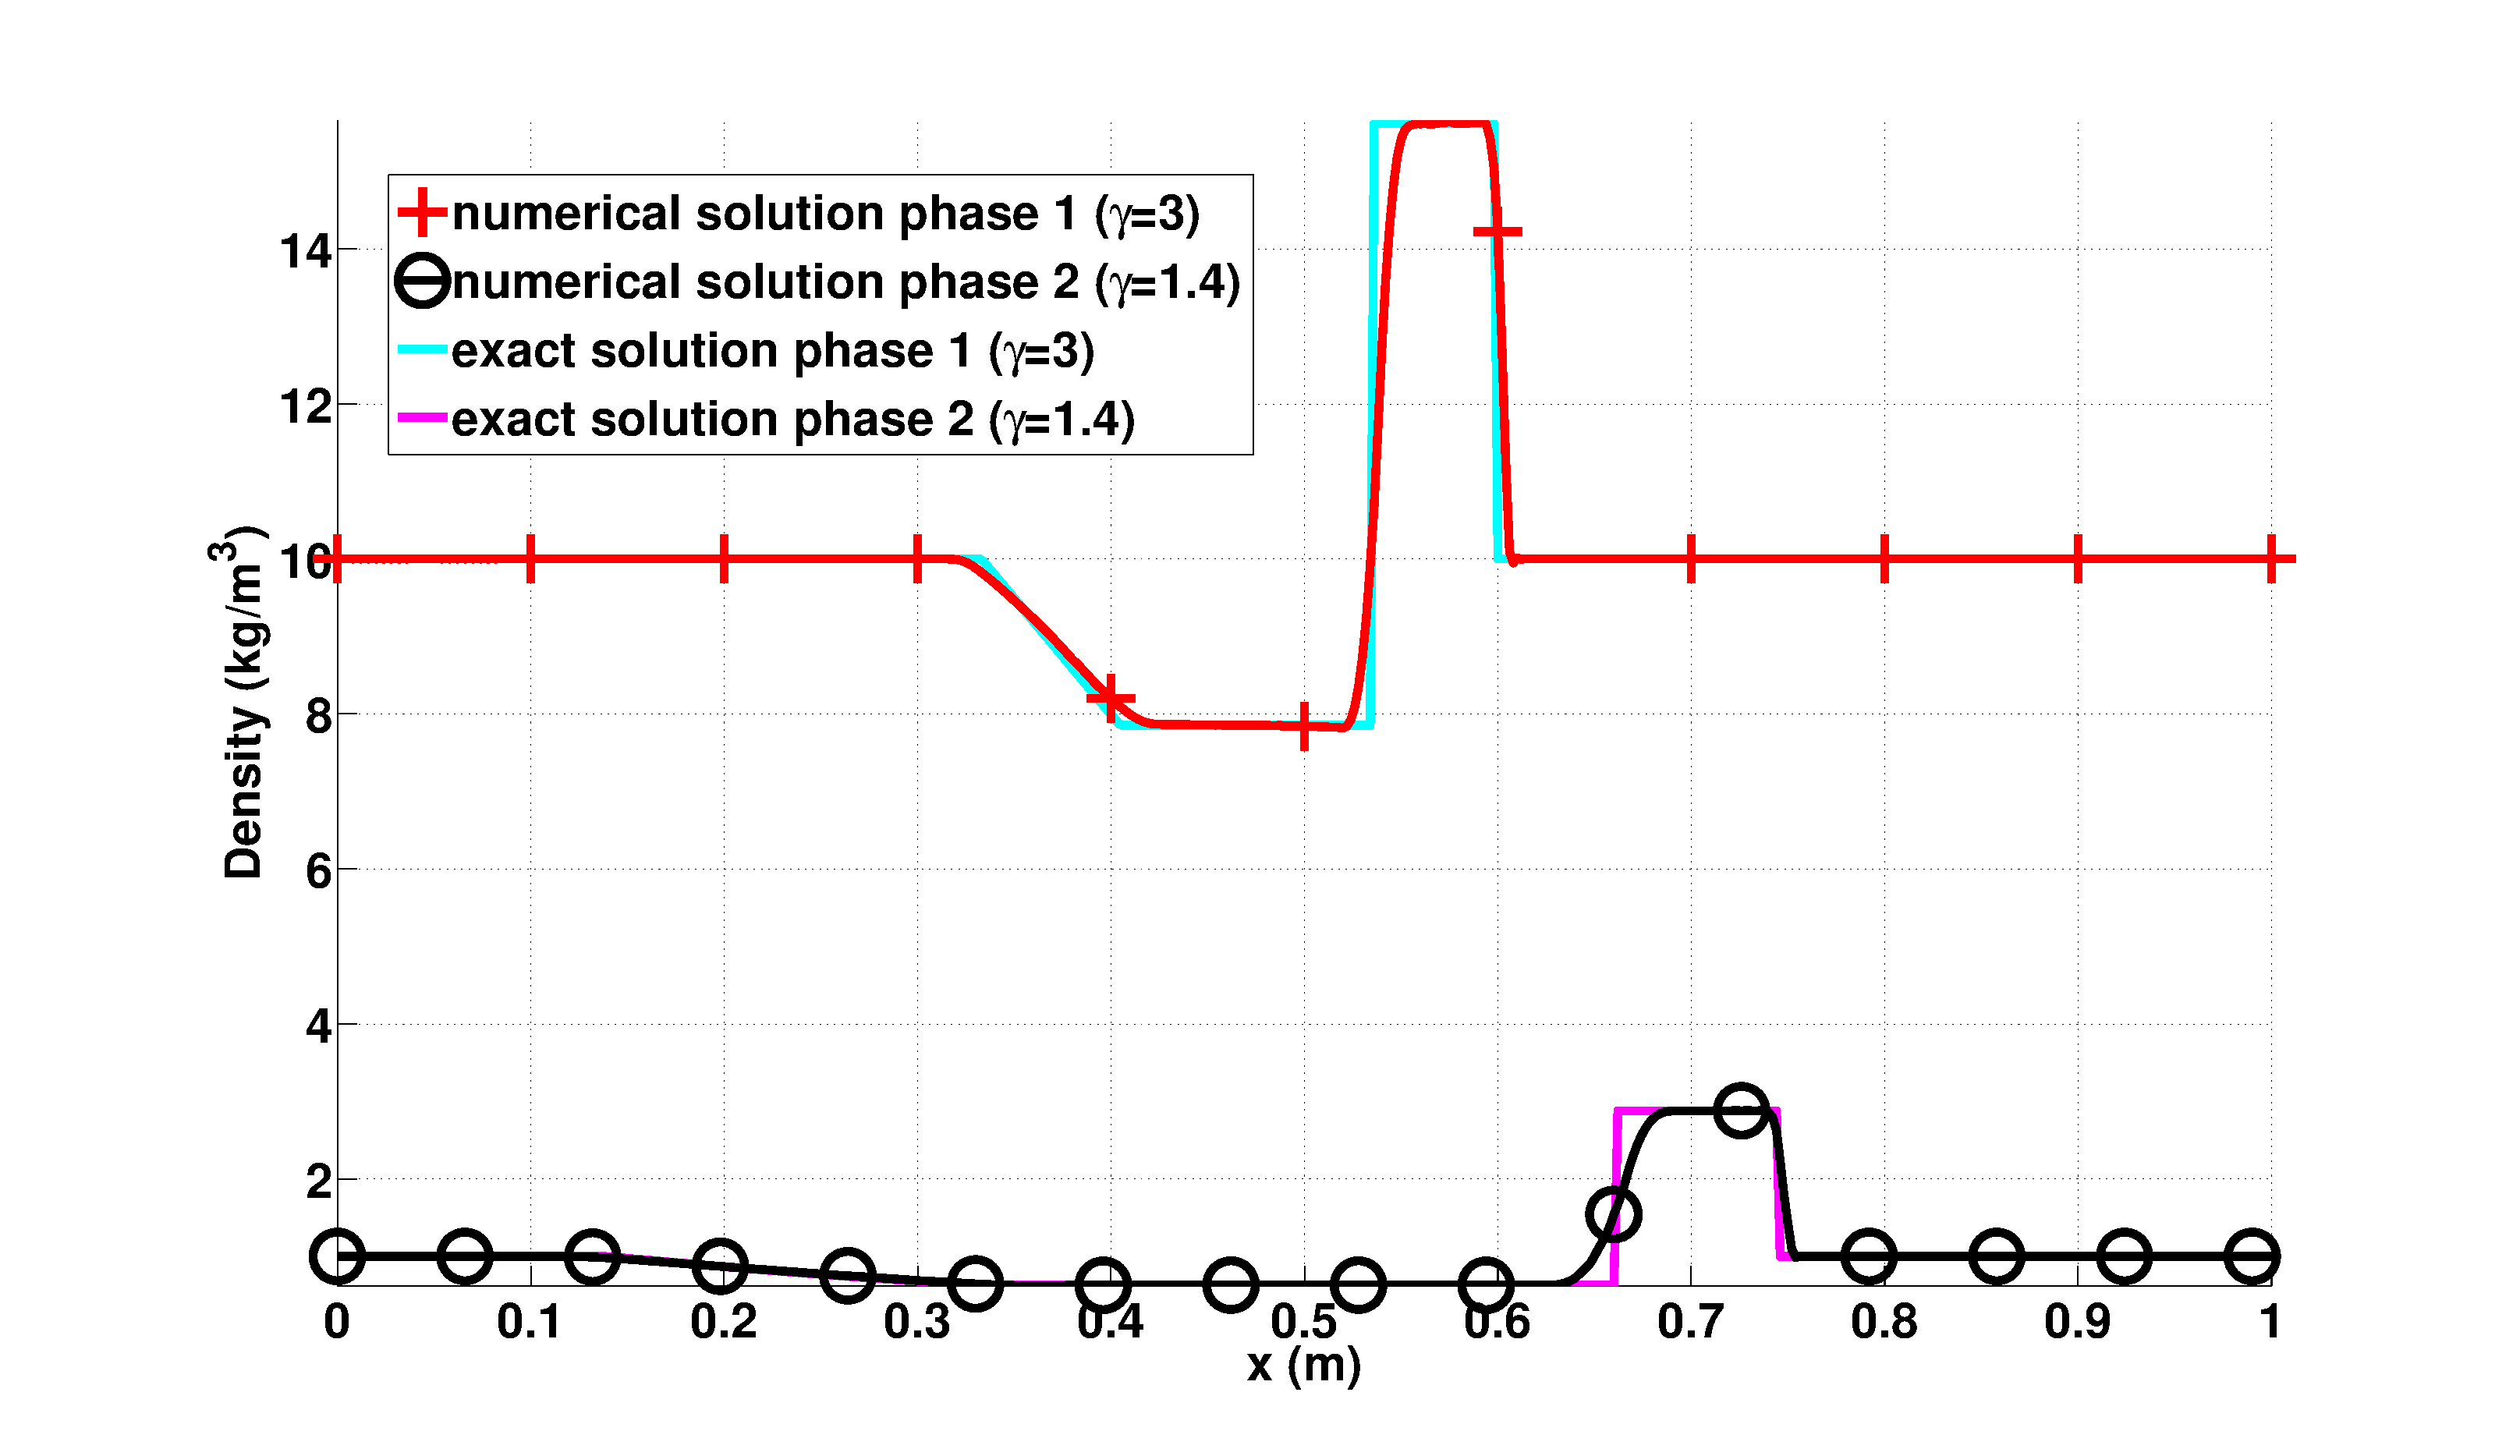
\includegraphics[width=\textwidth]{figures/two_phases_density.eps}
                \caption{Density}
                \label{fig:indp-phase-density}
        \end{subfigure}
        
        \begin{subfigure}[b]{0.495\textwidth}
                \centering
                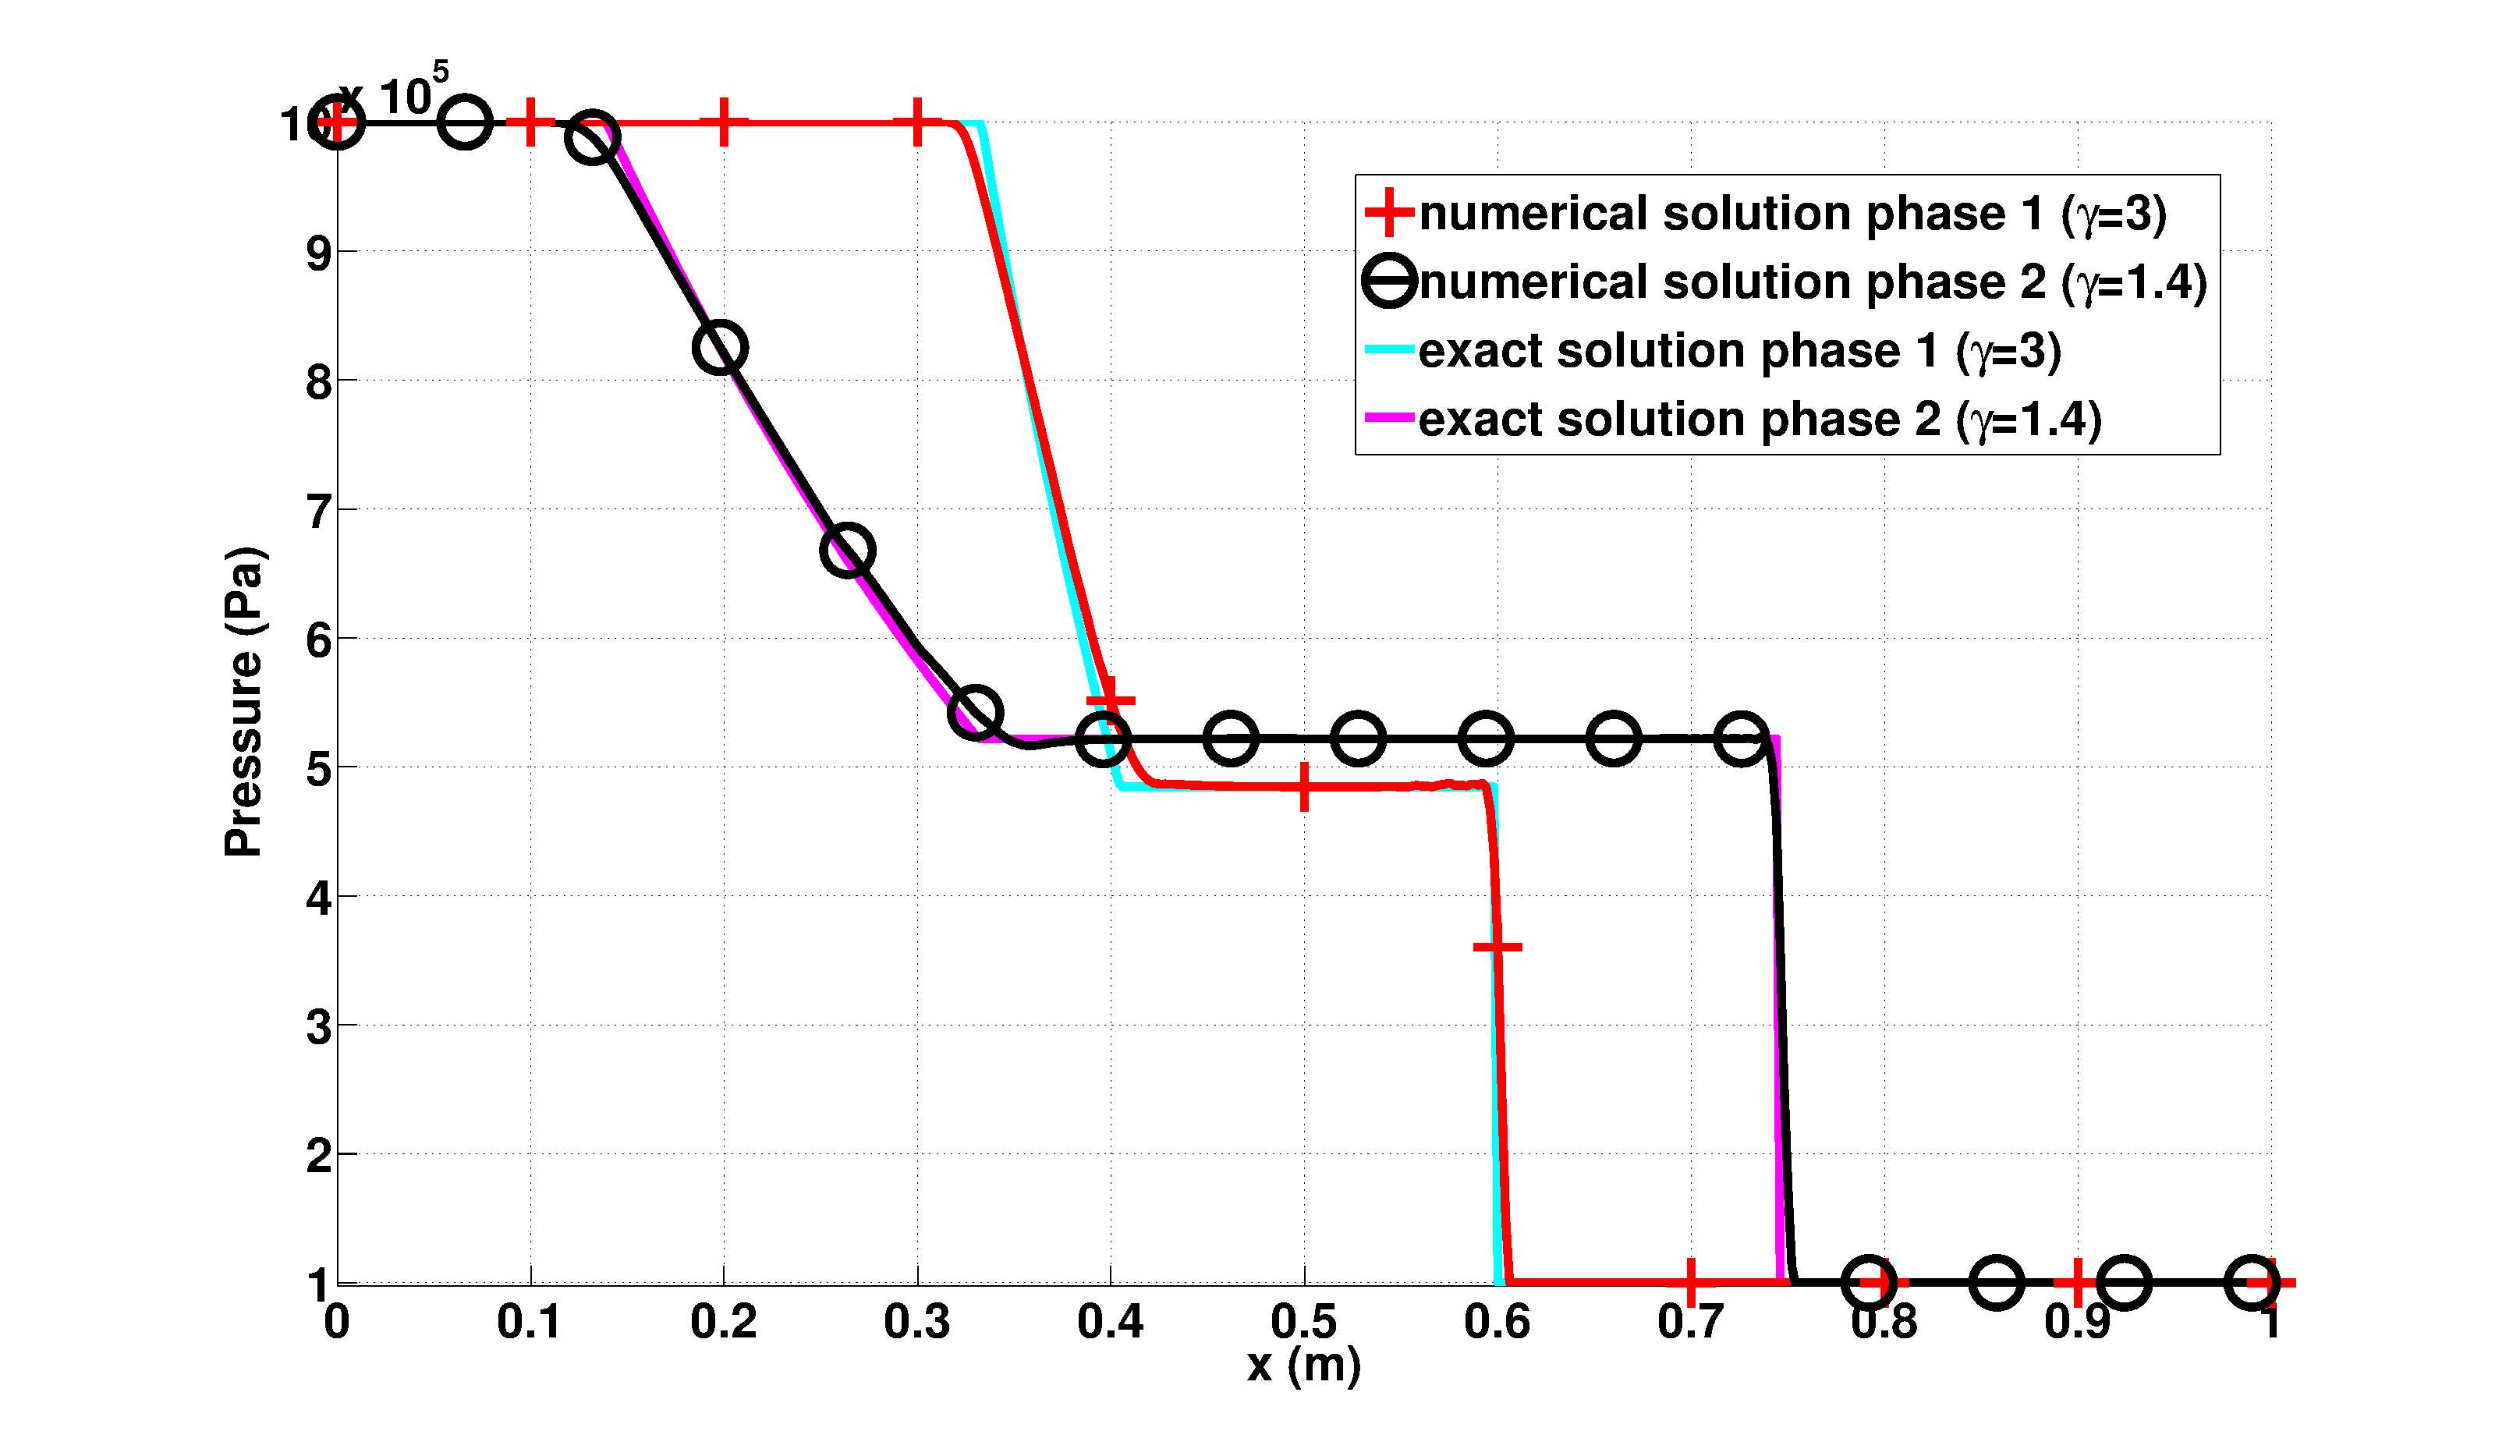
\includegraphics[width=\textwidth]{figures/two_phases_pressure.eps}
                \caption{Pressure}
                \label{fig:indp-phase-press}
        \end{subfigure}        
        \begin{subfigure}[b]{0.495\textwidth}
                \centering
                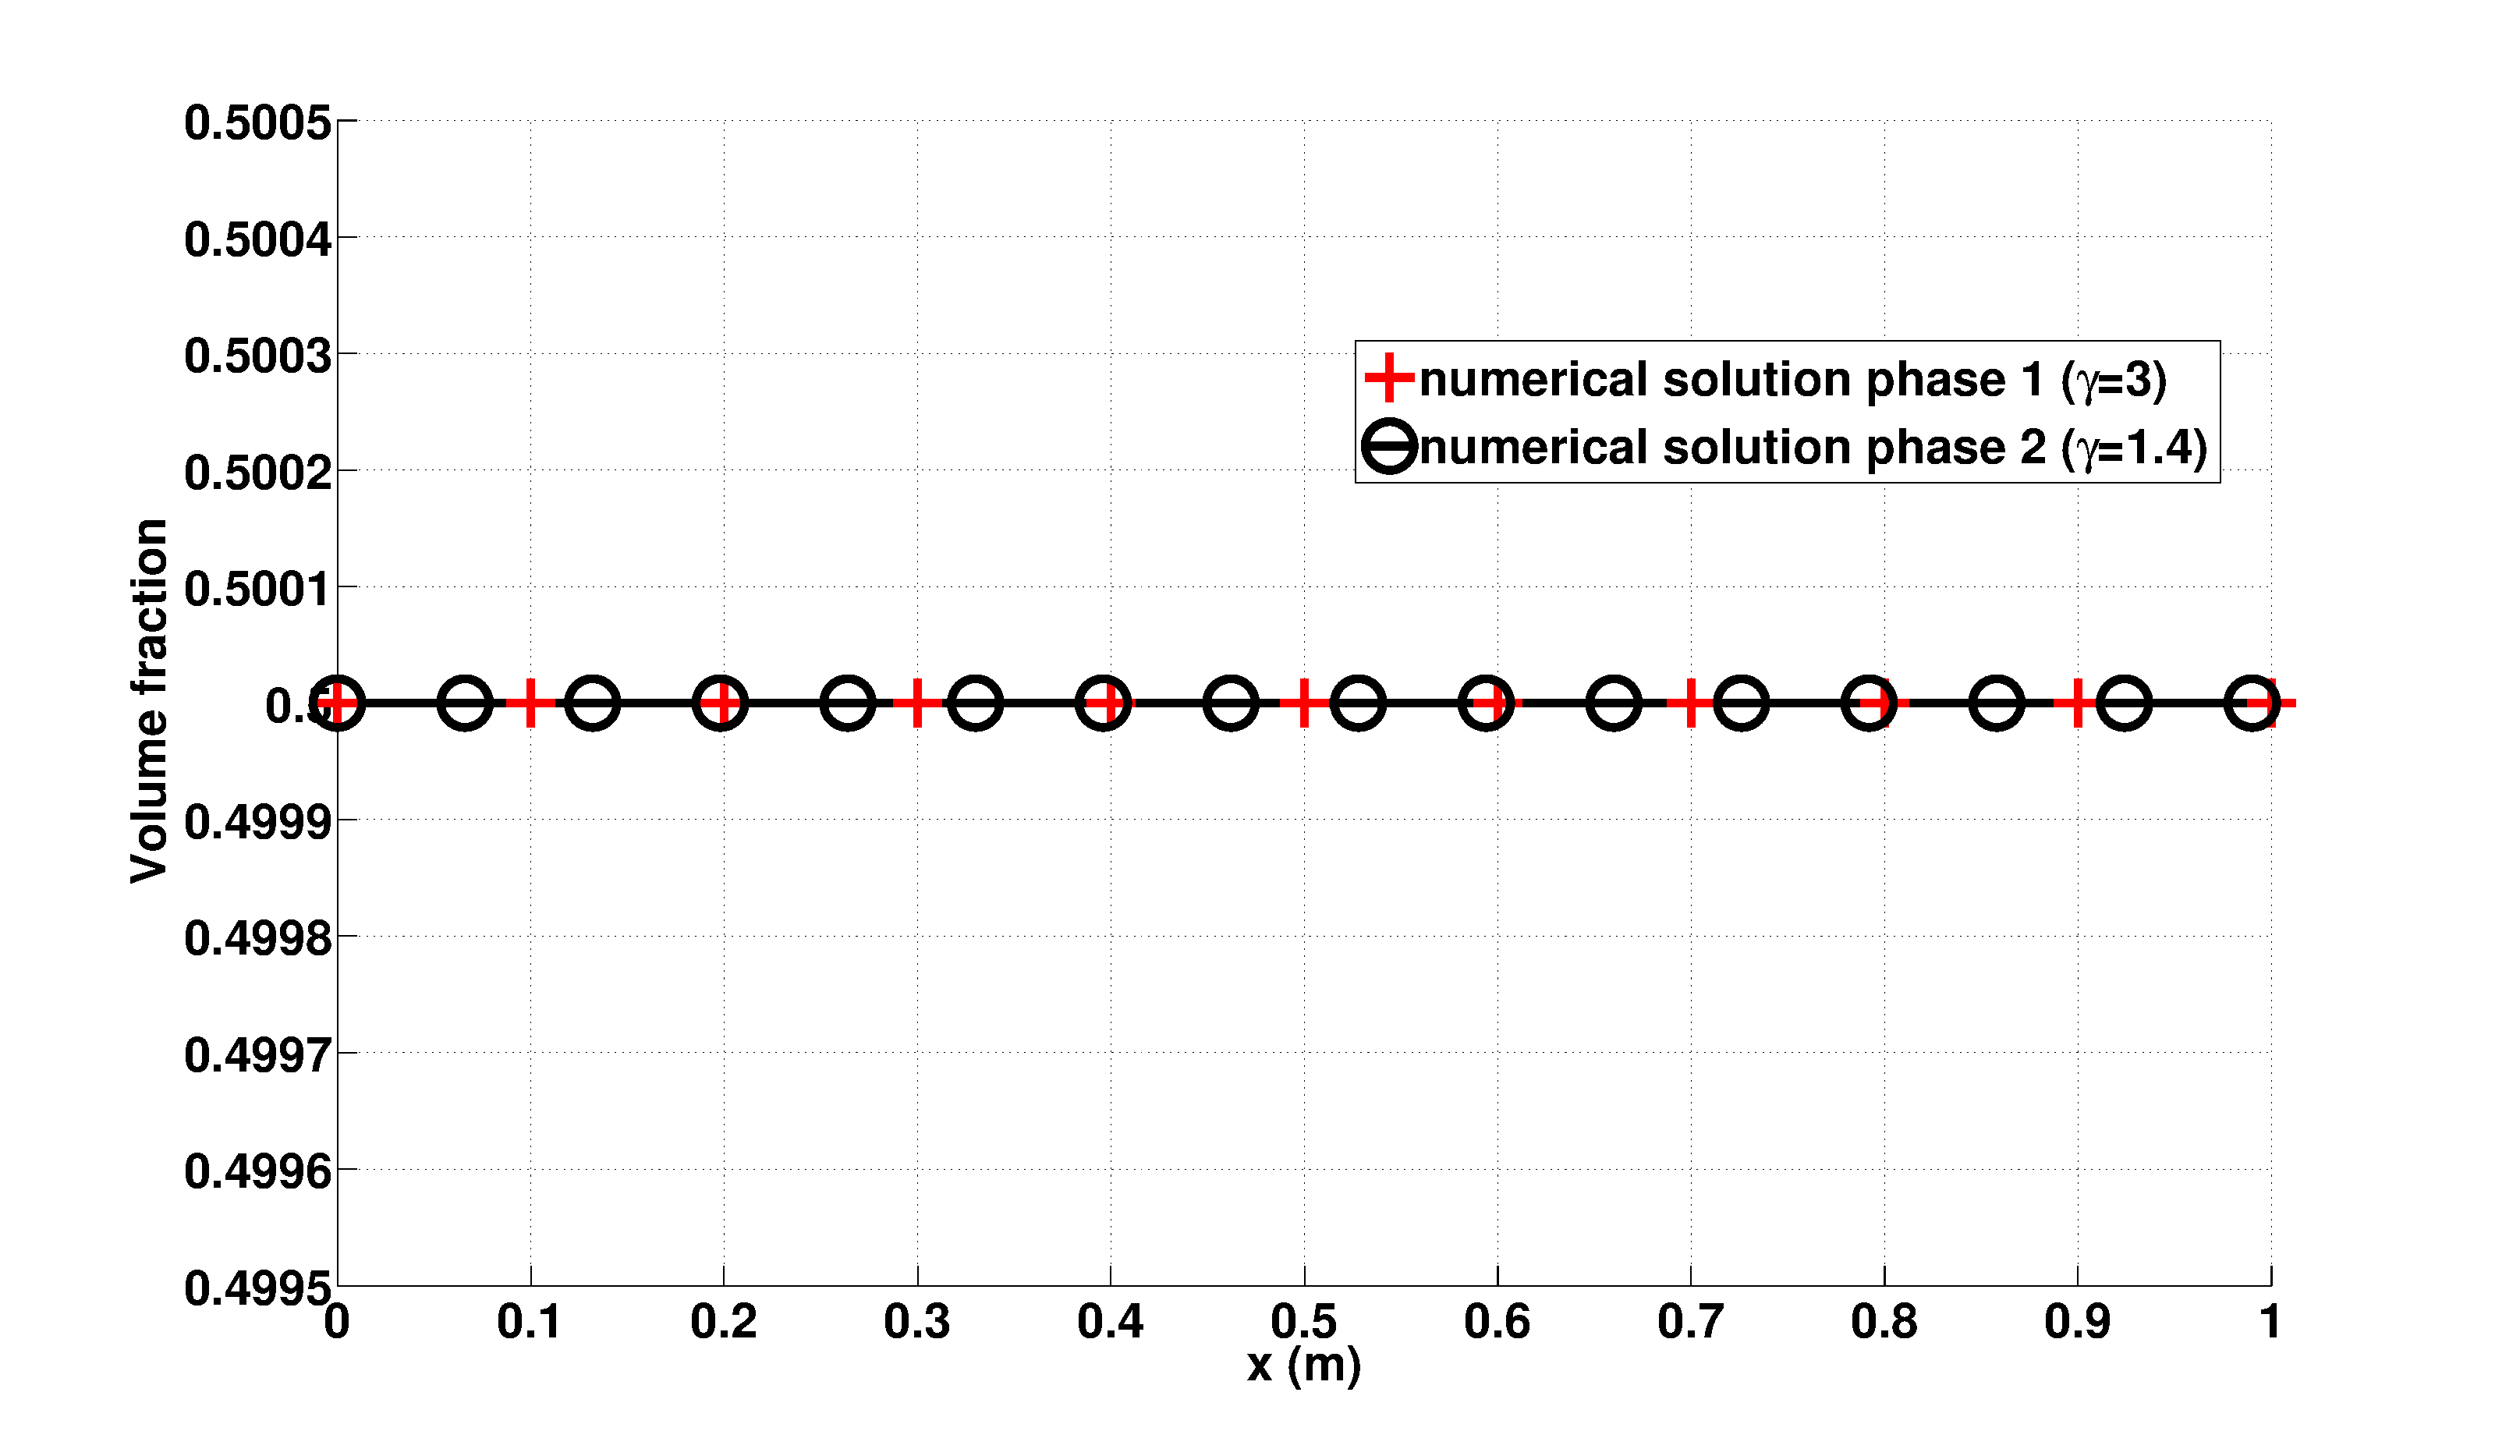
\includegraphics[width=\textwidth]{figures/two_phases_volume_fraction.eps}
                \caption{Volume fraction}
                \label{fig:indp-phase-vf}
        \end{subfigure}
        \caption{Numerical solution of a two-phase flow with large relaxation coefficients at $t=305 \ \mu s$.}\label{fig:indp-phase-variables}
\end{figure}
%
The velocity, density and pressure profiles given in \fig{fig:indp-phase-vel}, \fig{fig:indp-phase-density} and \fig{fig:indp-phase-press}, respectively, show good agreement with the exact solutions for both phases and also do not display any oscillations in the vicinity of the shock. The fluid $2$ is lighter and thus experiences stronger variations: its velocity is larger and the shock moves faster. The volume fraction remains constant during the transient and its profile is not altered by any mixture wave as shown in \fig{fig:indp-phase-vf}.
%
\begin{figure}[H]
        \centering
        \begin{subfigure}[b]{0.495\textwidth}
                \centering
                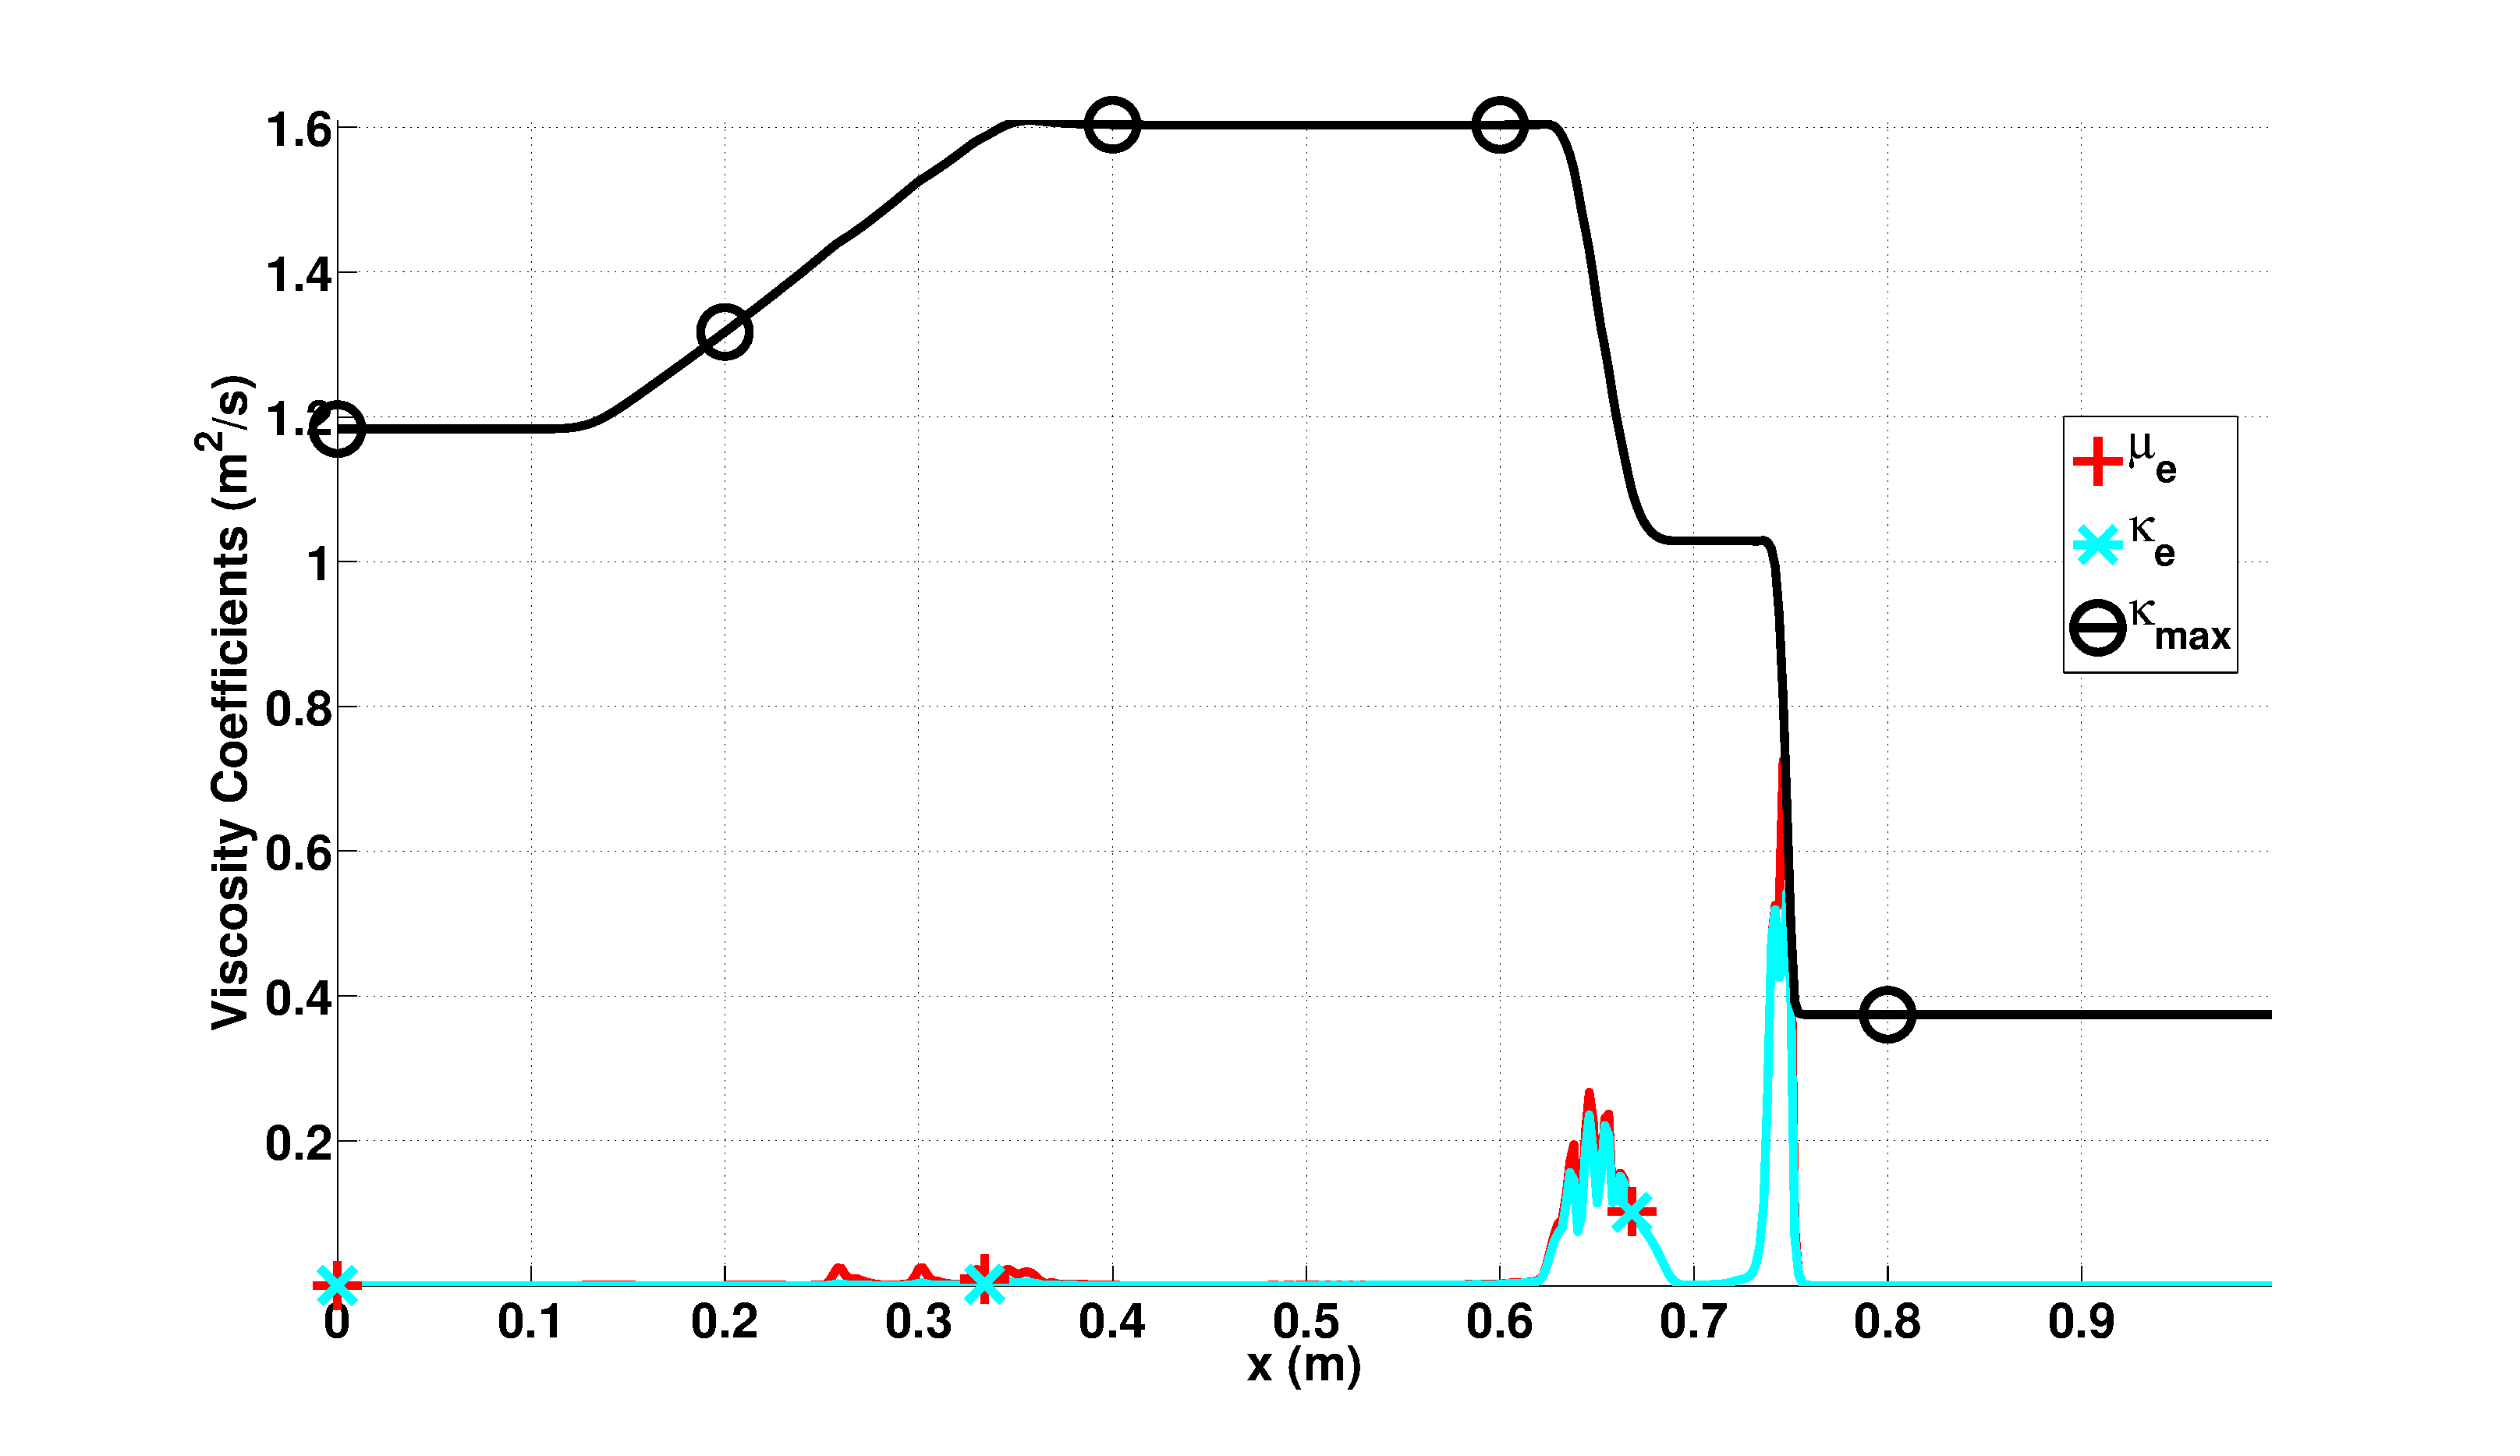
\includegraphics[width=\textwidth]{figures/two_phases_vapor_viscosity_kappa_mu.eps}
                \caption{Viscosity coefficients for phase 1.}
                \label{fig:indp-phase-1}
        \end{subfigure}%
        \begin{subfigure}[b]{0.495\textwidth}
                \centering
                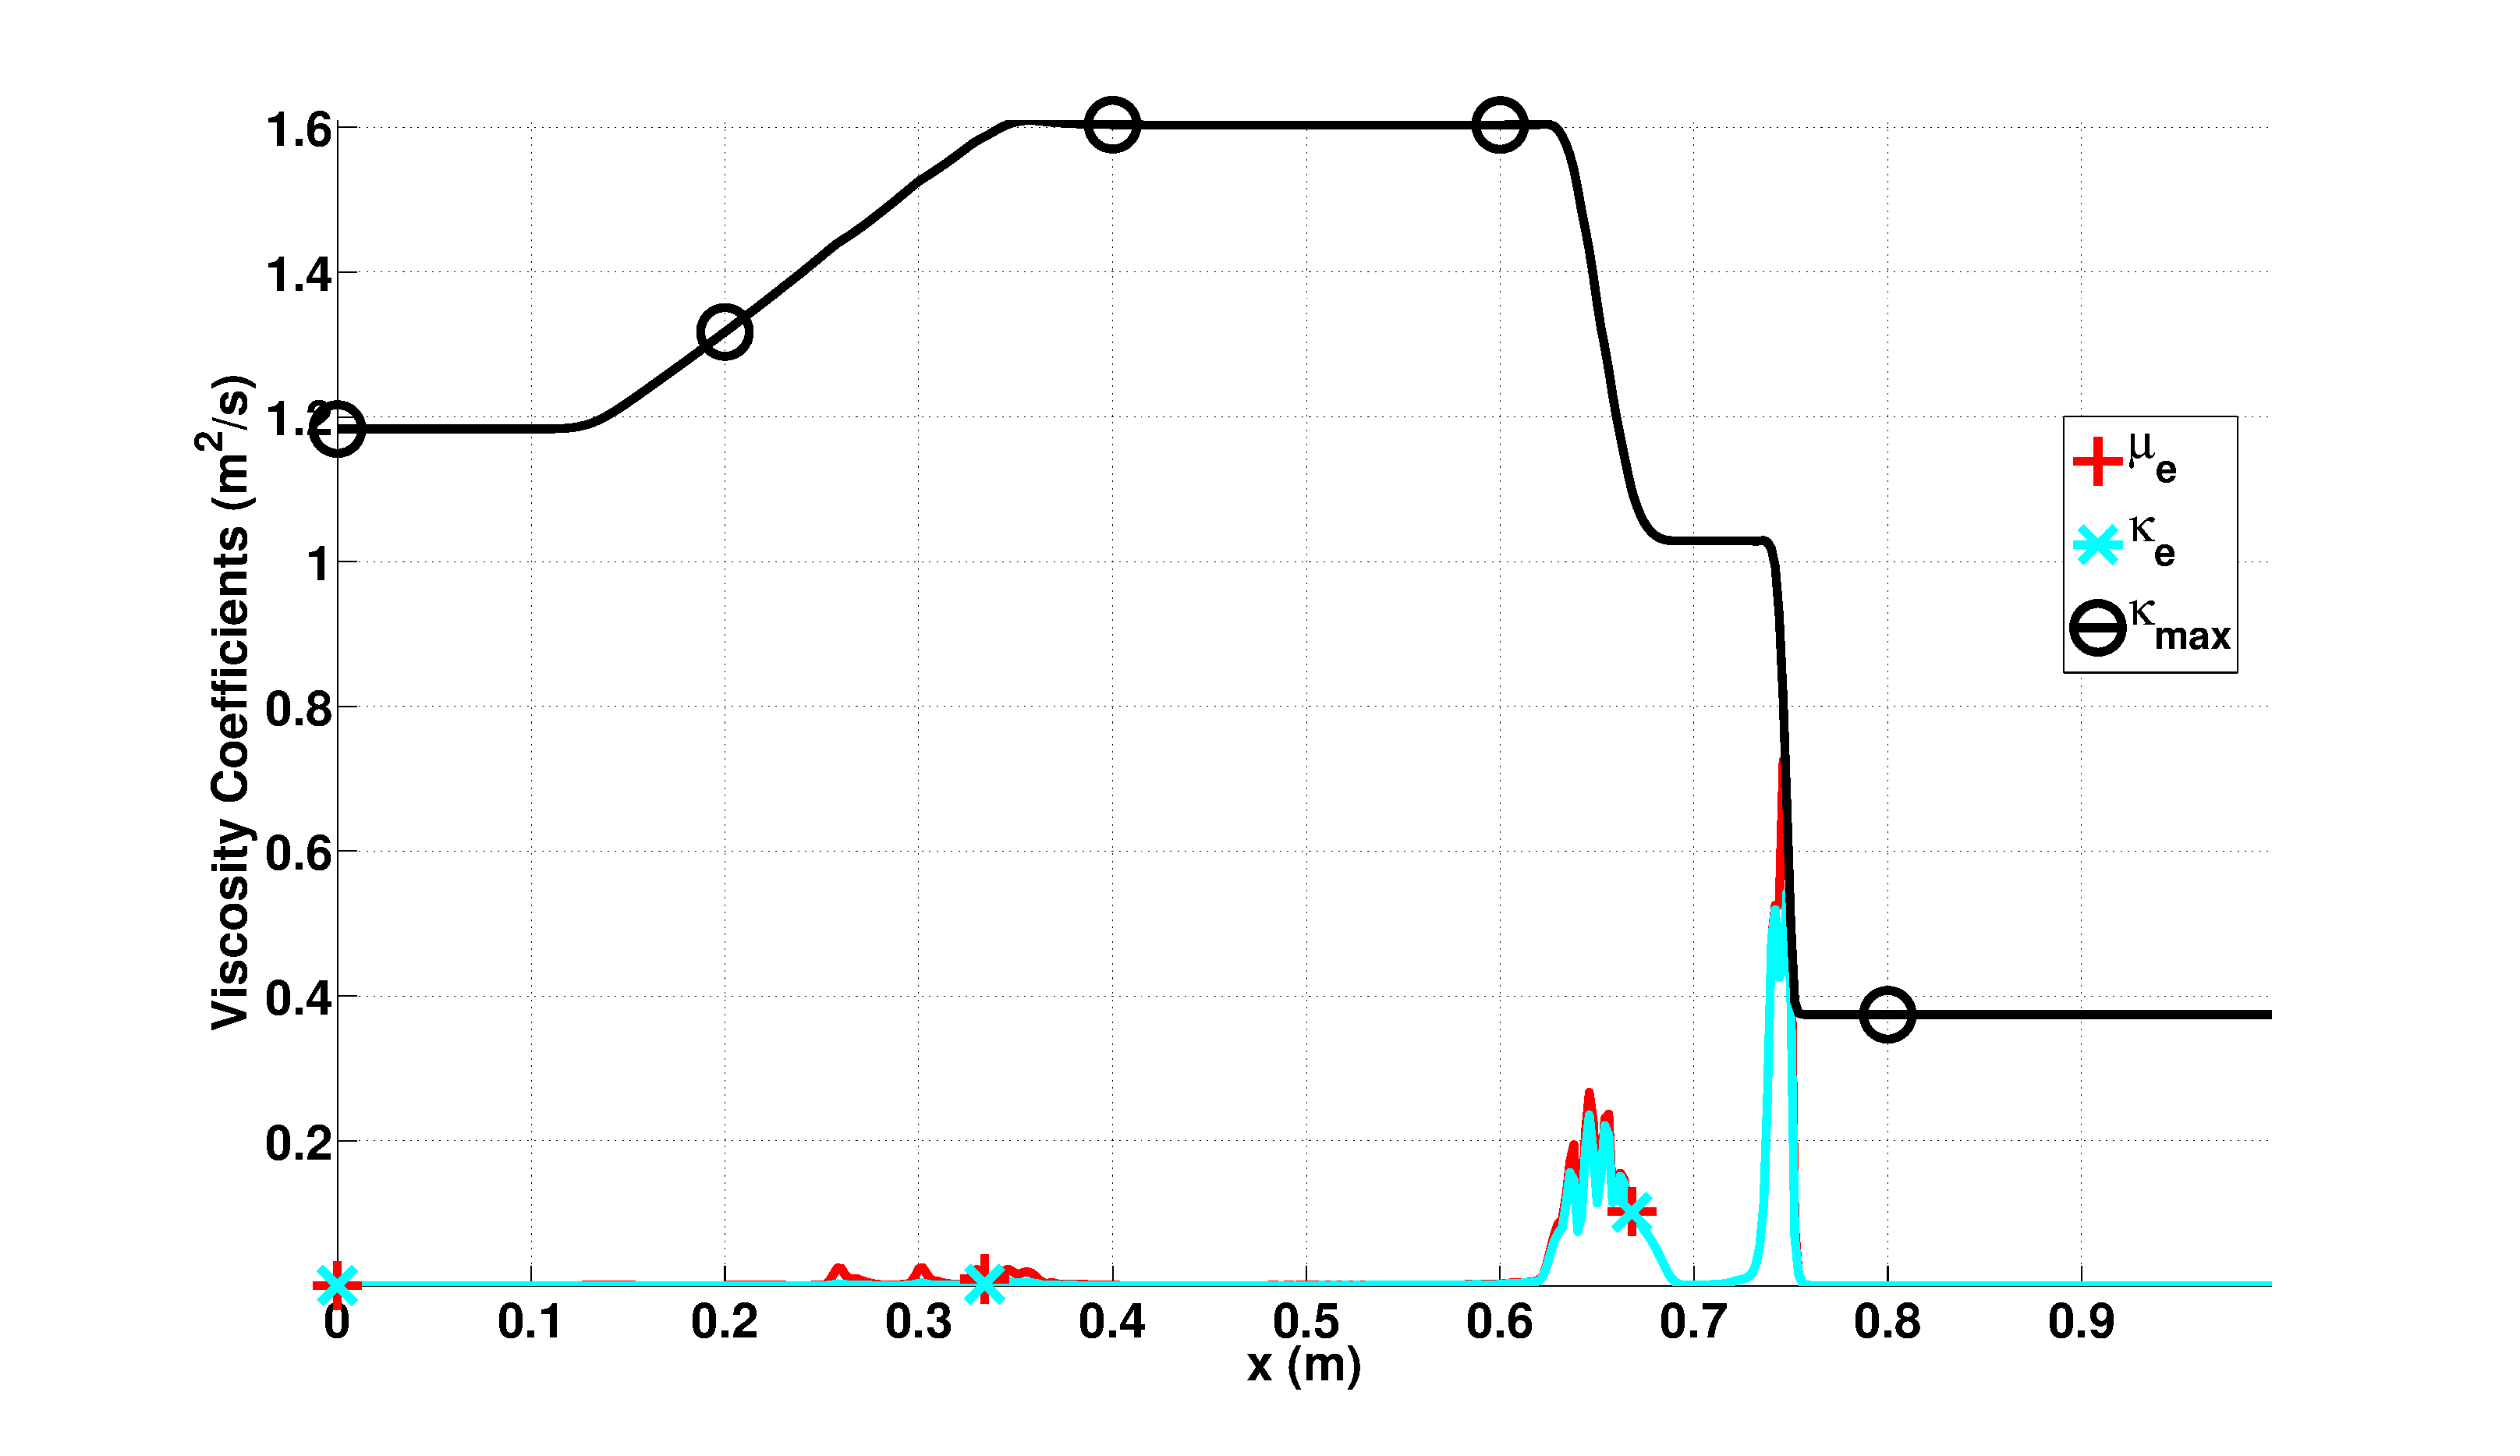
\includegraphics[width=\textwidth]{figures/two_phases_vapor_viscosity_kappa_mu.eps}
                \caption{Viscosity coefficients for phase 2}
                \label{fig:indp-phase-2}
        \end{subfigure}
        
        \begin{subfigure}[b]{0.495\textwidth}
                \centering
                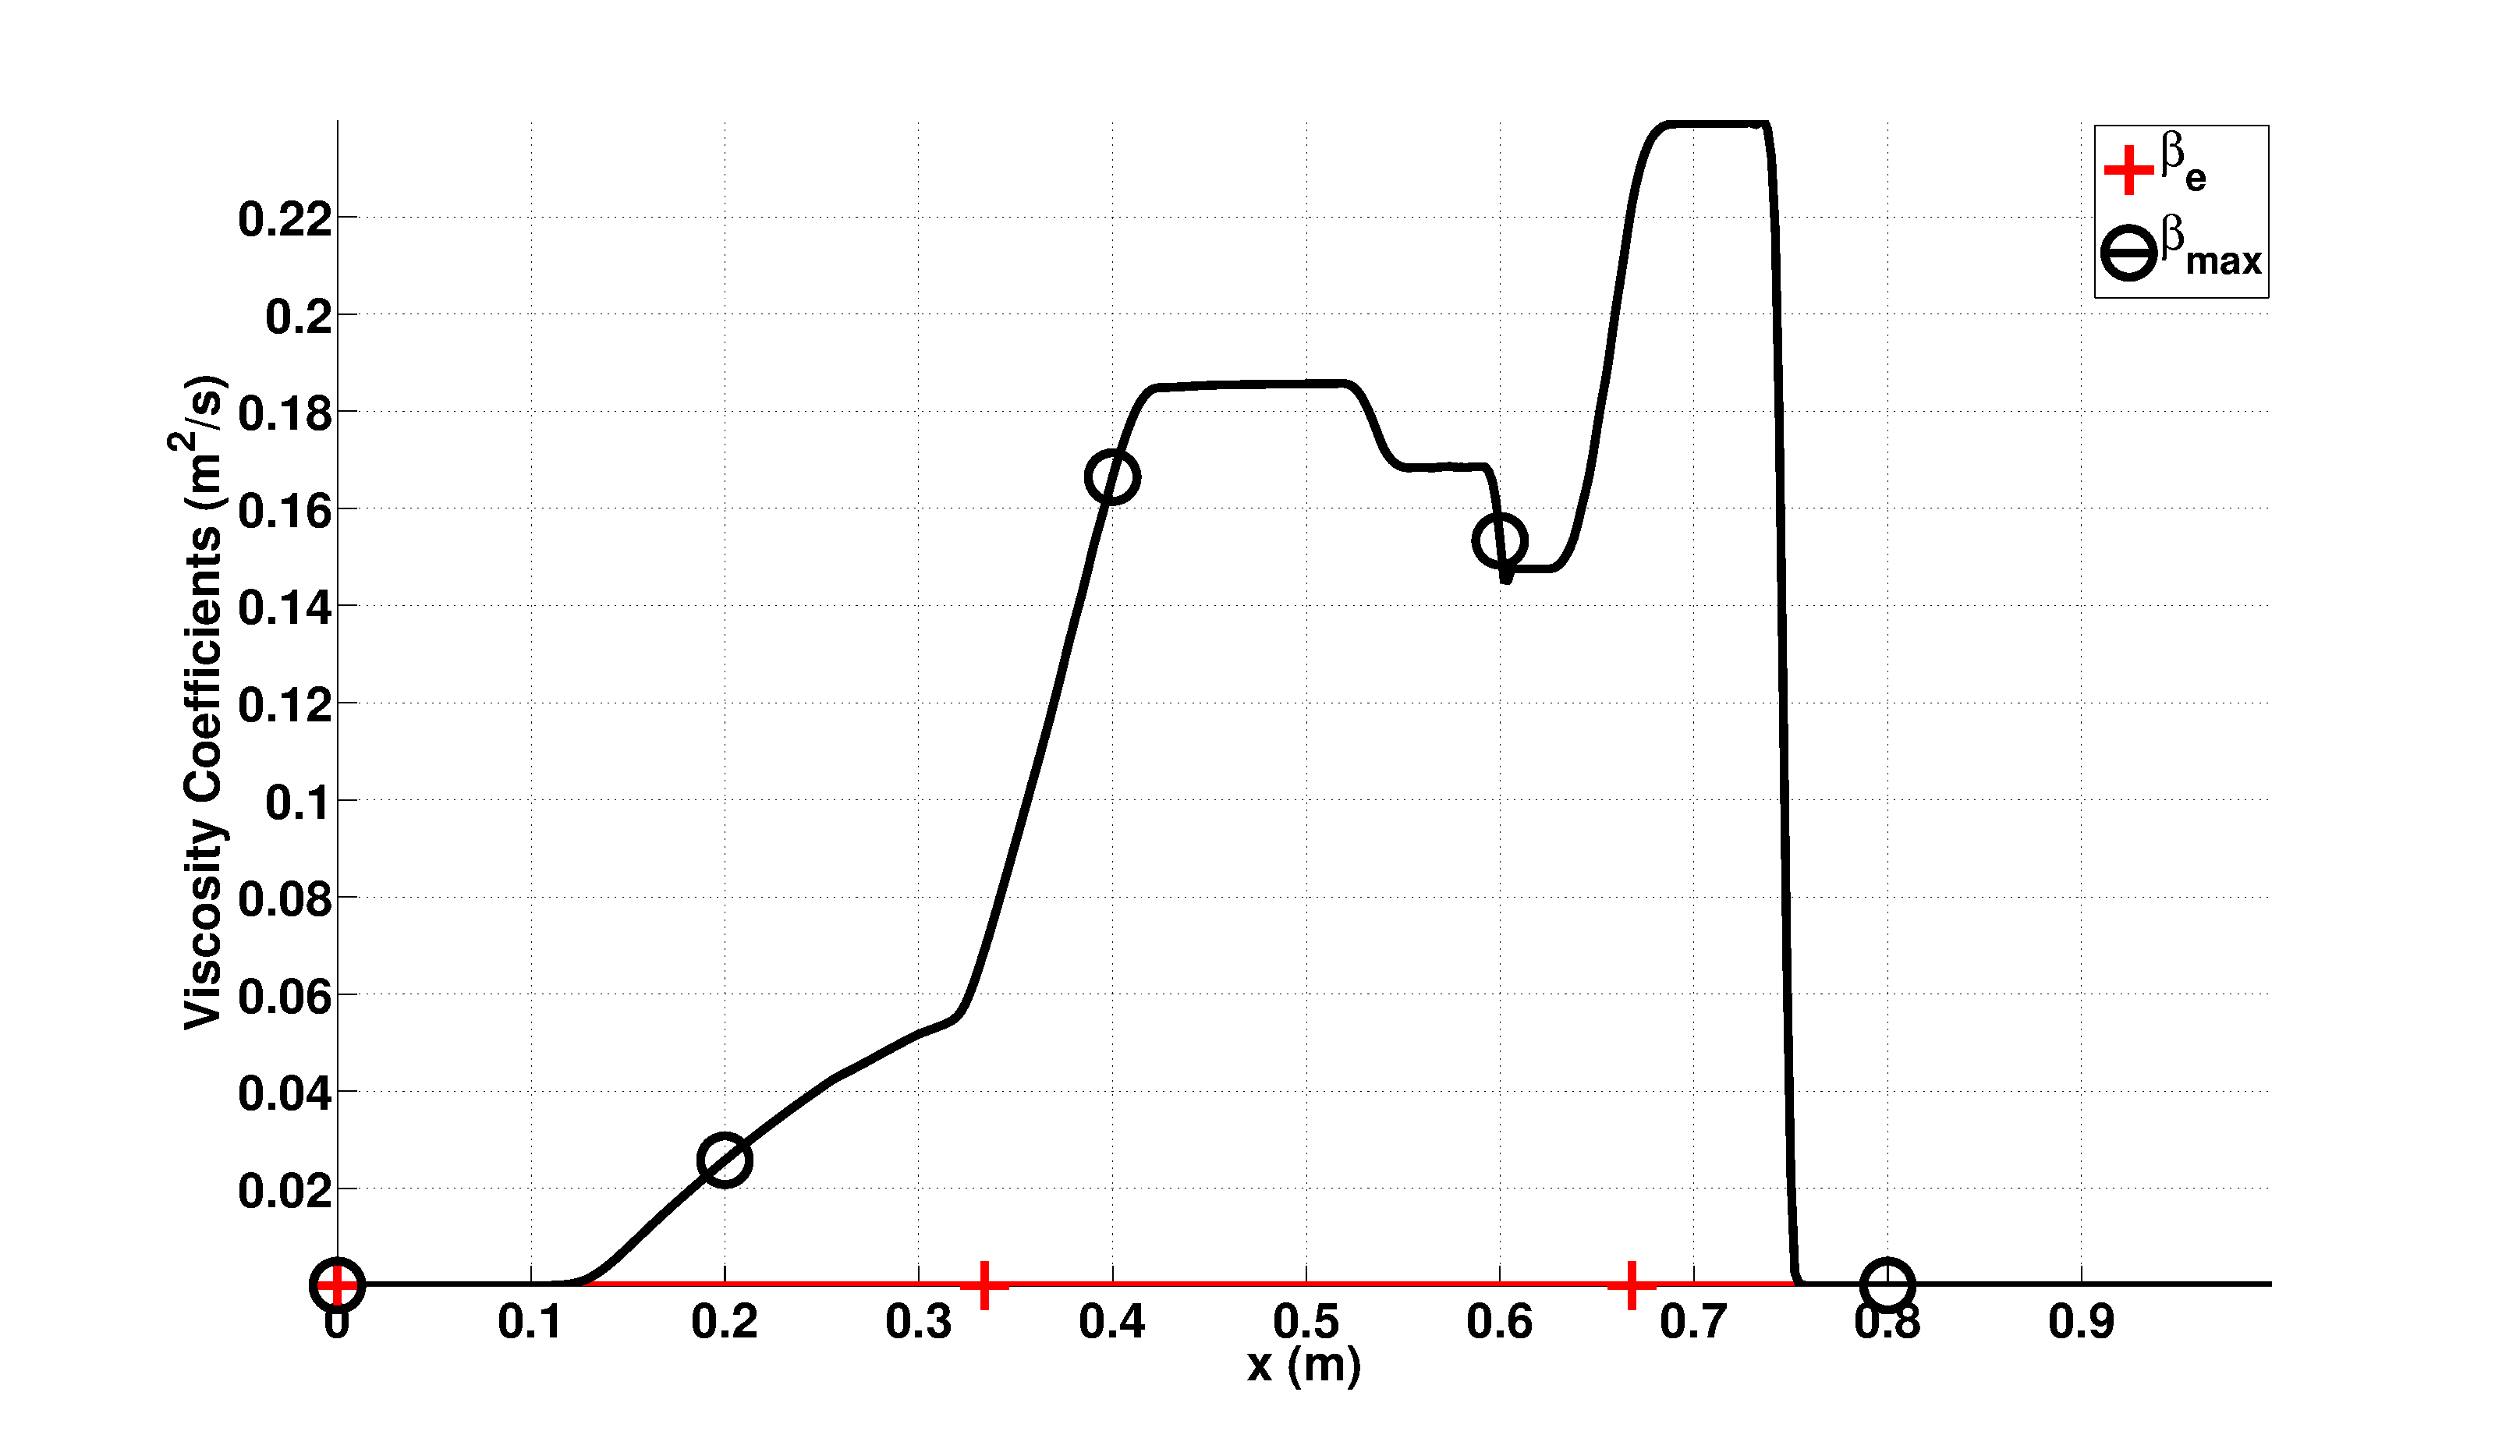
\includegraphics[width=\textwidth]{figures/two_phases_liquid_beta.eps}
                \caption{Viscosity coefficients for the volume fraction equation of phase 1.}
                \label{fig:indp-phase-beta}
        \end{subfigure}        
        \caption{Viscosity coefficients profiles for a two-phase flow with large relaxation coefficients at $t=305 \ \mu s$.}\label{fig:indp-phase-visc-coeff}
\end{figure}
%
The viscosity coefficients shown in \fig{fig:indp-phase-1} and \fig{fig:indp-phase-2} for both phases have similar profiles: they are peaked in the shock regions and also display a bump in the contact wave that is generated by the jump of the gradient of density (see \eqt{eq:jump-p-rho}). The viscosity coefficient $\beta_k$ computed from \eqt{eq:def-visc-sem} and used in the volume fraction equation is zero (\fig{fig:indp-phase-beta}) as expected since the volume fraction profile remains uniform. 
To demonstrate convergence of the numerical solution to the exact solution, a sequence of finer spatial meshes is employed. Because 
of the presence of a shock, second-order accuracy is not expected and the convergence rate of a numerical solution 
should be 1 and $1/2$ when measured in the L$_1$ and L$_2$ norms, respectively \cite{banks-jeffrey, majda-andrew}. 
Results are reported from \tbl{tbl:l1-norm-indp-phase-1} to \tbl{tbl:l2-norm-indp-phase-2} for the conservative variables (density, 
momentum and total energy). The convergence rates for the L$_1$ and L$_2$ norms of the error computed using \eqt{eq:conv_rates} 
are in good agreement with the theoretical values.
%Alike in \sct{sec:vf-advection-test}, we performed a convergence test by computing the L$_1$ and L$_2$ norms of the error between the numerical and exact solutions. Once again, the exact solution was obtained from a Riemann solver (REF). The L$_1$ and L$_2$ norms of the error between the numerical and exact solution, and the convergence rate are given from \tbl{tbl:l1-norm-indp-phase-1} to \tbl{tbl:l2-norm-indp-phase-2} for the conservative variables of phases 1 and 2: density, momentum and total energy.
%
\begin{table}[H]
\begin{center}
 \caption{\label{tbl:l1-norm-indp-phase-1} L$_1$ norm of the error for phase 1.}
 \begin{tabular}{|c|c|c|c|c|c|c|c|c|}
 \hline
cells & density         & rate   & momentum        & rate    & total energy         & rate     \\ \hline
25      & 4.2753735 $10^{-1}$ & $-$    & 8.4705 $10^{5}$ & $-$     & 7.2737           & $-$      \\ \hline
50      & 1.5115549 $10^{-1}$ & 1.07 & 4.7893 $10^{5}$ & 0.82 & 6.1493           & 0.24 \\ \hline
100    & 2.9373 $10^{-2}$ & 2.18 & 1.0613 $10^{5}$ & 2.17  & 1.2275           & 2.32   \\ \hline
200    & 5.1120 $10^{-3}$ & 2.52 & 1.8446 $10^{4}$ & 2.52  & 1.8943 $10^{-1}$ & 2.69   \\ \hline
400    & 1.0558 $10^{-3}$ & 2.28 & 3.7938 $10^{3}$ & 2.28  & 3.7919 $10^{-2}$ & 2.32   \\ \hline
800    & 2.3712 $10^{-4}$ & 2.15 & 8.4471 $10^{2}$ & 2.17  & 8.5517 $10^{-3}$ & 2.15   \\ \hline
1600  & 5.6058 $10^{-5}$ & 2.08 & 1.9839 $10^{2}$ & 2.09  & 2.0475 $10^{-3}$ & 2.06   \\ \hline
3200  & 1.3278 $10^{-5}$ & $2.08$ & 4.6622 $10^{1}$ & 2.09  & 4.9516 $10^{-4}$ & $2.04$   \\ \hline
\end{tabular}
\end{center}
\end{table}
%
%
\begin{table}[H]
\begin{center}
 \caption{\label{tbl:l2-norm-indp-phase-1} L$_2$ norm of the error for phase 1.}
 \begin{tabular}{|c|c|c|c|c|c|c|c|c|}
 \hline
cells& density            & rate & momentum          & rate & total energy           & rate \\ \hline
25      & 2.8037 $10^{-1}$ & $-$    & 8.4705 $10^{5}$ & $-$     & 7.2737           & $-$      \\ \hline
50      & 1.3343 $10^{-1}$ & 1.07 & 4.7893 $10^{5}$ & 0.82 & 6.1493           & 0.24 \\ \hline
100    & 2.9373 $10^{-2}$ & 2.18 & 1.0613 $10^{5}$ & 2.17  & 1.2275           & 2.32   \\ \hline
200    & 5.1120 $10^{-3}$ & 2.52 & 1.8446 $10^{4}$ & 2.52  & 1.8943 $10^{-1}$ & 2.69   \\ \hline
400    & 1.0558 $10^{-3}$ & 2.28 & 3.7938 $10^{3}$ & 2.28  & 3.7919 $10^{-2}$ & 2.32   \\ \hline
800    & 2.3712 $10^{-4}$ & 2.15 & 8.4471 $10^{2}$ & 2.17  & 8.5517 $10^{-3}$ & 2.15   \\ \hline
1600  & 5.6058 $10^{-5}$ & 2.08 & 1.9839 $10^{2}$ & 2.09  & 2.0475 $10^{-3}$ & 2.06   \\ \hline
3200  & 1.3278 $10^{-5}$ & $2.08$ & 4.6622 $10^{1}$ & 2.09  & 4.9516 $10^{-4}$ & $2.04$   \\ \hline
\end{tabular}
\end{center}
\end{table}
%
\begin{table}[H]
\begin{center}
 \caption{\label{tbl:l1-norm-indp-phase-2} L$_1$ norm of the error for phase 2.}
 \begin{tabular}{|c|c|c|c|c|c|c|c|c|}
 \hline
cells & density         & rate   & momentum        & rate    & total energy         & rate     \\ \hline
25      & 2.8037 $10^{-1}$ & $-$    & 8.4705 $10^{5}$ & $-$     & 7.2737           & $-$      \\ \hline
50      & 1.3343 $10^{-1}$ & 1.07 & 4.7893 $10^{5}$ & 0.82 & 6.1493           & 0.24 \\ \hline
100    & 2.9373 $10^{-2}$ & 2.18 & 1.0613 $10^{5}$ & 2.17  & 1.2275           & 2.32   \\ \hline
200    & 5.1120 $10^{-3}$ & 2.52 & 1.8446 $10^{4}$ & 2.52  & 1.8943 $10^{-1}$ & 2.69   \\ \hline
400    & 1.0558 $10^{-3}$ & 2.28 & 3.7938 $10^{3}$ & 2.28  & 3.7919 $10^{-2}$ & 2.32   \\ \hline
800    & 2.3712 $10^{-4}$ & 2.15 & 8.4471 $10^{2}$ & 2.17  & 8.5517 $10^{-3}$ & 2.15   \\ \hline
1600  & 5.6058 $10^{-5}$ & 2.08 & 1.9839 $10^{2}$ & 2.09  & 2.0475 $10^{-3}$ & 2.06   \\ \hline
3200  & 1.3278 $10^{-5}$ & $2.08$ & 4.6622 $10^{1}$ & 2.09  & 4.9516 $10^{-4}$ & $2.04$   \\ \hline
\end{tabular}
\end{center}
\end{table}
%
%
\begin{table}[H]
\begin{center}
 \caption{\label{tbl:l2-norm-indp-phase-2} L$_2$ norm of the error for phase 2.}
 \begin{tabular}{|c|c|c|c|c|c|c|c|c|}
 \hline
cells& density            & rate & momentum          & rate & total energy           & rate \\ \hline
25      & 2.8037 $10^{-1}$ & $-$    & 8.4705 $10^{5}$ & $-$     & 7.2737           & $-$      \\ \hline
50      & 1.3343 $10^{-1}$ & 1.07 & 4.7893 $10^{5}$ & 0.82 & 6.1493           & 0.24 \\ \hline
100    & 2.9373 $10^{-2}$ & 2.18 & 1.0613 $10^{5}$ & 2.17  & 1.2275           & 2.32   \\ \hline
200    & 5.1120 $10^{-3}$ & 2.52 & 1.8446 $10^{4}$ & 2.52  & 1.8943 $10^{-1}$ & 2.69   \\ \hline
400    & 1.0558 $10^{-3}$ & 2.28 & 3.7938 $10^{3}$ & 2.28  & 3.7919 $10^{-2}$ & 2.32   \\ \hline
800    & 2.3712 $10^{-4}$ & 2.15 & 8.4471 $10^{2}$ & 2.17  & 8.5517 $10^{-3}$ & 2.15   \\ \hline
1600  & 5.6058 $10^{-5}$ & 2.08 & 1.9839 $10^{2}$ & 2.09  & 2.0475 $10^{-3}$ & 2.06   \\ \hline
3200  & 1.3278 $10^{-5}$ & $2.08$ & 4.6622 $10^{1}$ & 2.09  & 4.9516 $10^{-4}$ & $2.04$   \\ \hline
\end{tabular}
\end{center}
\end{table}
%
%density
%L1_rate_liq =
%
%   0.698474584175195
%   0.874510385731901
%   0.814824861178414
%   0.815970206565530
%   0.896076568308733
%   0.705208737360476
%
%
%L2_rate_liq =
%
%   0.442350653268543
%   0.522223100273032
%   0.398259522190196
%   0.383544020028946
%   0.513418419987055
%   0.378165192636462
%
%
%L1_rate_gas =
%
%   0.619532837665265
%   0.862588950544313
%   0.745834496626933
%   0.749808458532859
%   0.749308416912120
%   0.252295273303110
%
%
%L2_rate_gas =
%
%   0.357778843433264
%   0.483001570610292
%   0.339833894216642
%   0.369110354923374
%   0.465968067404870
%   0.143248053323787
%
%momentum
%L1_rate_liq =
%
%   0.737688156190138
%   0.896945663436033
%   0.863430489721563
%   0.884595324483929
%   0.960341081814526
%   0.694640793274355
%
%
%L2_rate_liq =
%
%   0.434602377569489
%   0.521631679213127
%   0.489942505425969
%   0.500217888006692
%   0.644781123357885
%   0.602011393365698
%
%
%L1_rate_gas =
%
%   0.678746095870472
%   0.885526625333708
%   0.762829013690574
%   0.769256729869945
%   0.676020388766989
%   0.211853870320983
%
%
%L2_rate_gas =
%
%   0.397859595661207
%   0.544224820073587
%   0.363005135237459
%   0.390095105196733
%   0.422498425942370
%   0.109587979500658
%
%energy
%L1_rate_liq =
%
%   0.836791451455638
%   0.914134005898690
%   0.899000357593017
%   0.921534650880842
%   0.978451199178983
%   0.591917552011068
%
%
%L2_rate_liq =
%
%   0.516467635119108
%   0.544927040186610
%   0.538068453112055
%   0.565187263949209
%   0.745617472277509
%   0.532064999635494
%
%
%L1_rate_gas =
%
%   0.803181250184597
%   0.984434154440203
%   0.856575051766479
%   0.852291371065551
%   0.557934272979114
%   0.186438681447322
%
%
%L2_rate_gas =
%
%   0.463694707907407
%   0.789666576586823
%   0.509273596388979
%   0.546572510988959
%   0.281892382344974
%   0.012598650453265
%
%%%%%%%%%%%%%%%%%%%%%%%%%%%%%%%%%%%%%
\subsubsection{Shock tube of two fluids with infinite relaxation coefficients}\label{sec:shock-tube-infinite-rel-coeff}
%%%%%%%%%%%%%%%%%%%%%%%%%%%%%%%%%%%%%
%
Once again, we consider a 1-D shock tube with the same initial conditions and the same fluids as in \sct{sec:vf-advection-test} and \sct{sec:shock-tube-two-indep-fluids}. 
The pressure and velocity relaxation coefficients are no longer set to zero but computed from \eqt{eq:Aint-def} and \eqt{E-R:86} with $A_{int,max} =  
10^4$ $m^{-1}$: $\mu_P \sim 4$ and $\lambda_u \sim 5 \times 10^5$ $s^{-1}$. The values of the relaxation coefficients are large enough to make the 
relaxation terms dominant in the momentum and energy equations of each phase (see \eqt{eq:multi-7-eqn-mom} and \eqt{eq:multi-7-eqn-energy}). Thus, the two fluids will exhibit the 
same pressure and velocity. The volume fraction will not remain uniform but is expected to vary due to the pressure relaxation source term (\eqt{eqn:multi-d-7-eqn-liq-vol}). For 
this test, an exact solution is not available but the reader can refer to \cite{Saurel_2007} for a comparison. An uniform mesh of 500 cells is used. The code is 
run until $t = 305$ $\mu s$ with a CFL of one. The numerical solutions (pressure, velocity, density and volume fraction) of the phases $1$ and $2$ are presented in \fig{fig:inf-rel-variables} along with the viscosity coefficient profiles in \fig{fig:inf-rel-visc-coeff} for each phase. Dirichlet boundary conditions are once again used.
%
\begin{figure}[H]
        \centering
        \begin{subfigure}[b]{0.495\textwidth}
                \centering
                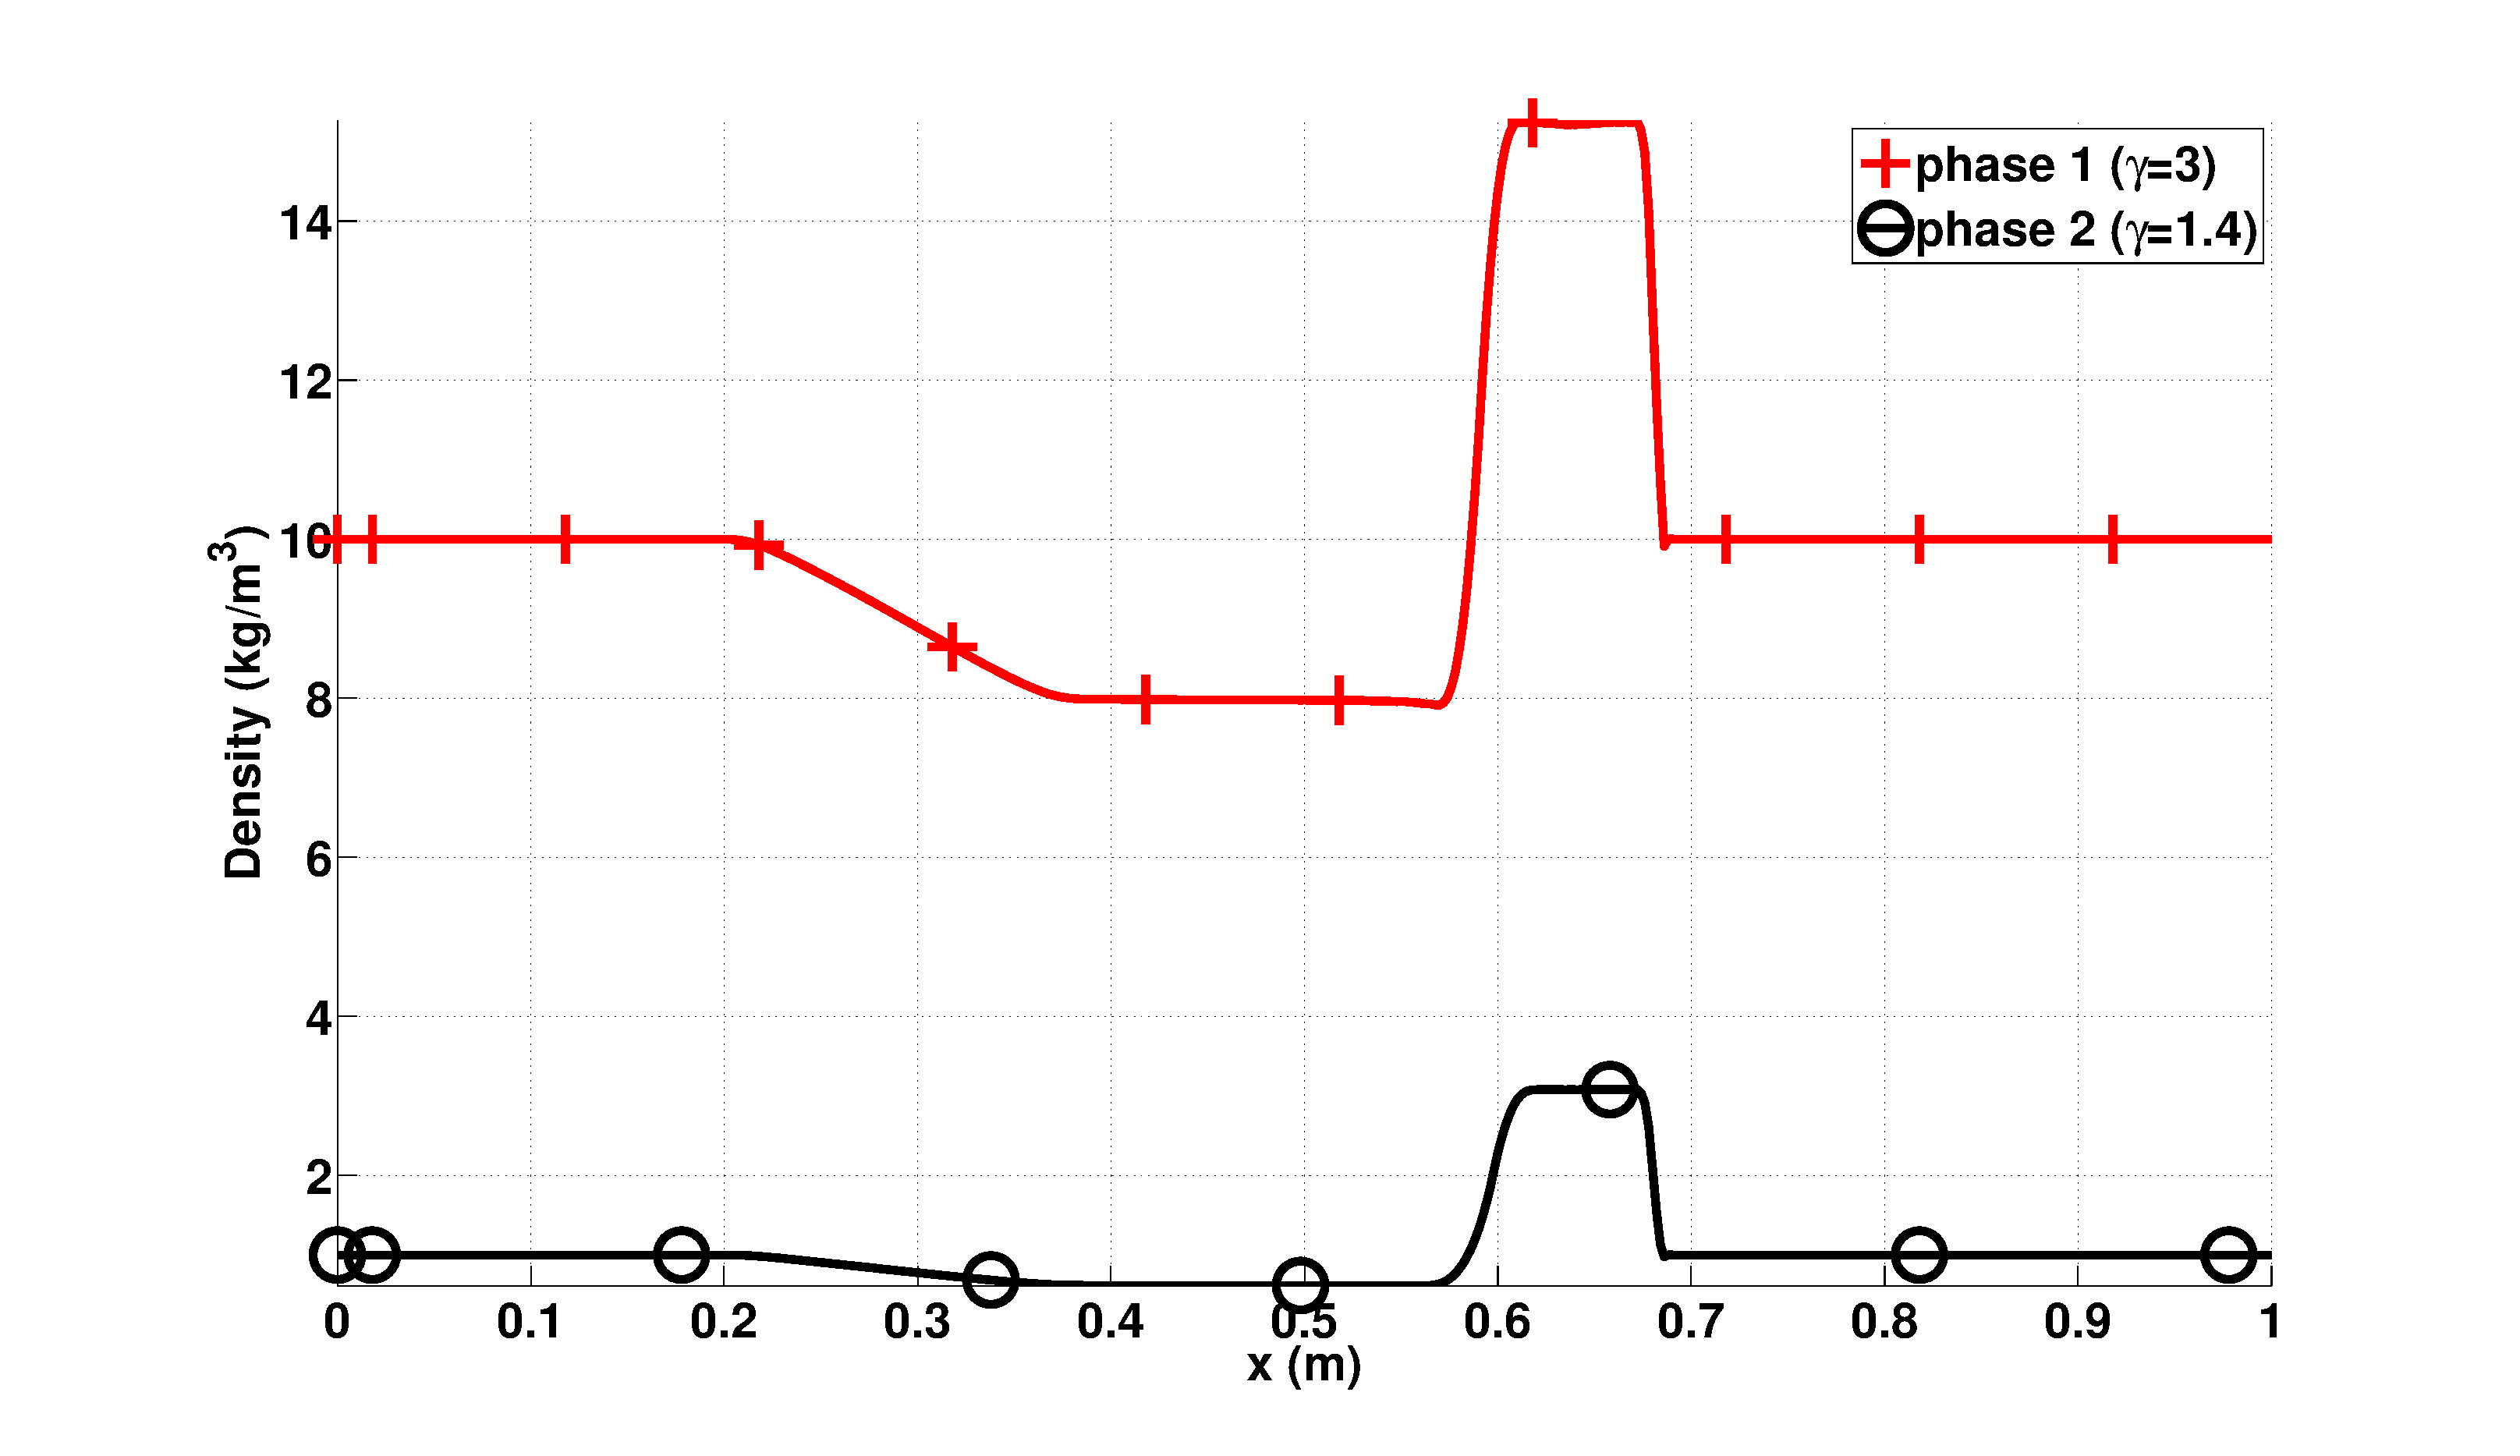
\includegraphics[width=\textwidth]{figures/relaxation_two_phases_density.eps}
                \caption{Velocity}
                \label{fig:inf-rel-vel}
        \end{subfigure}%
        \begin{subfigure}[b]{0.495\textwidth}
                \centering
                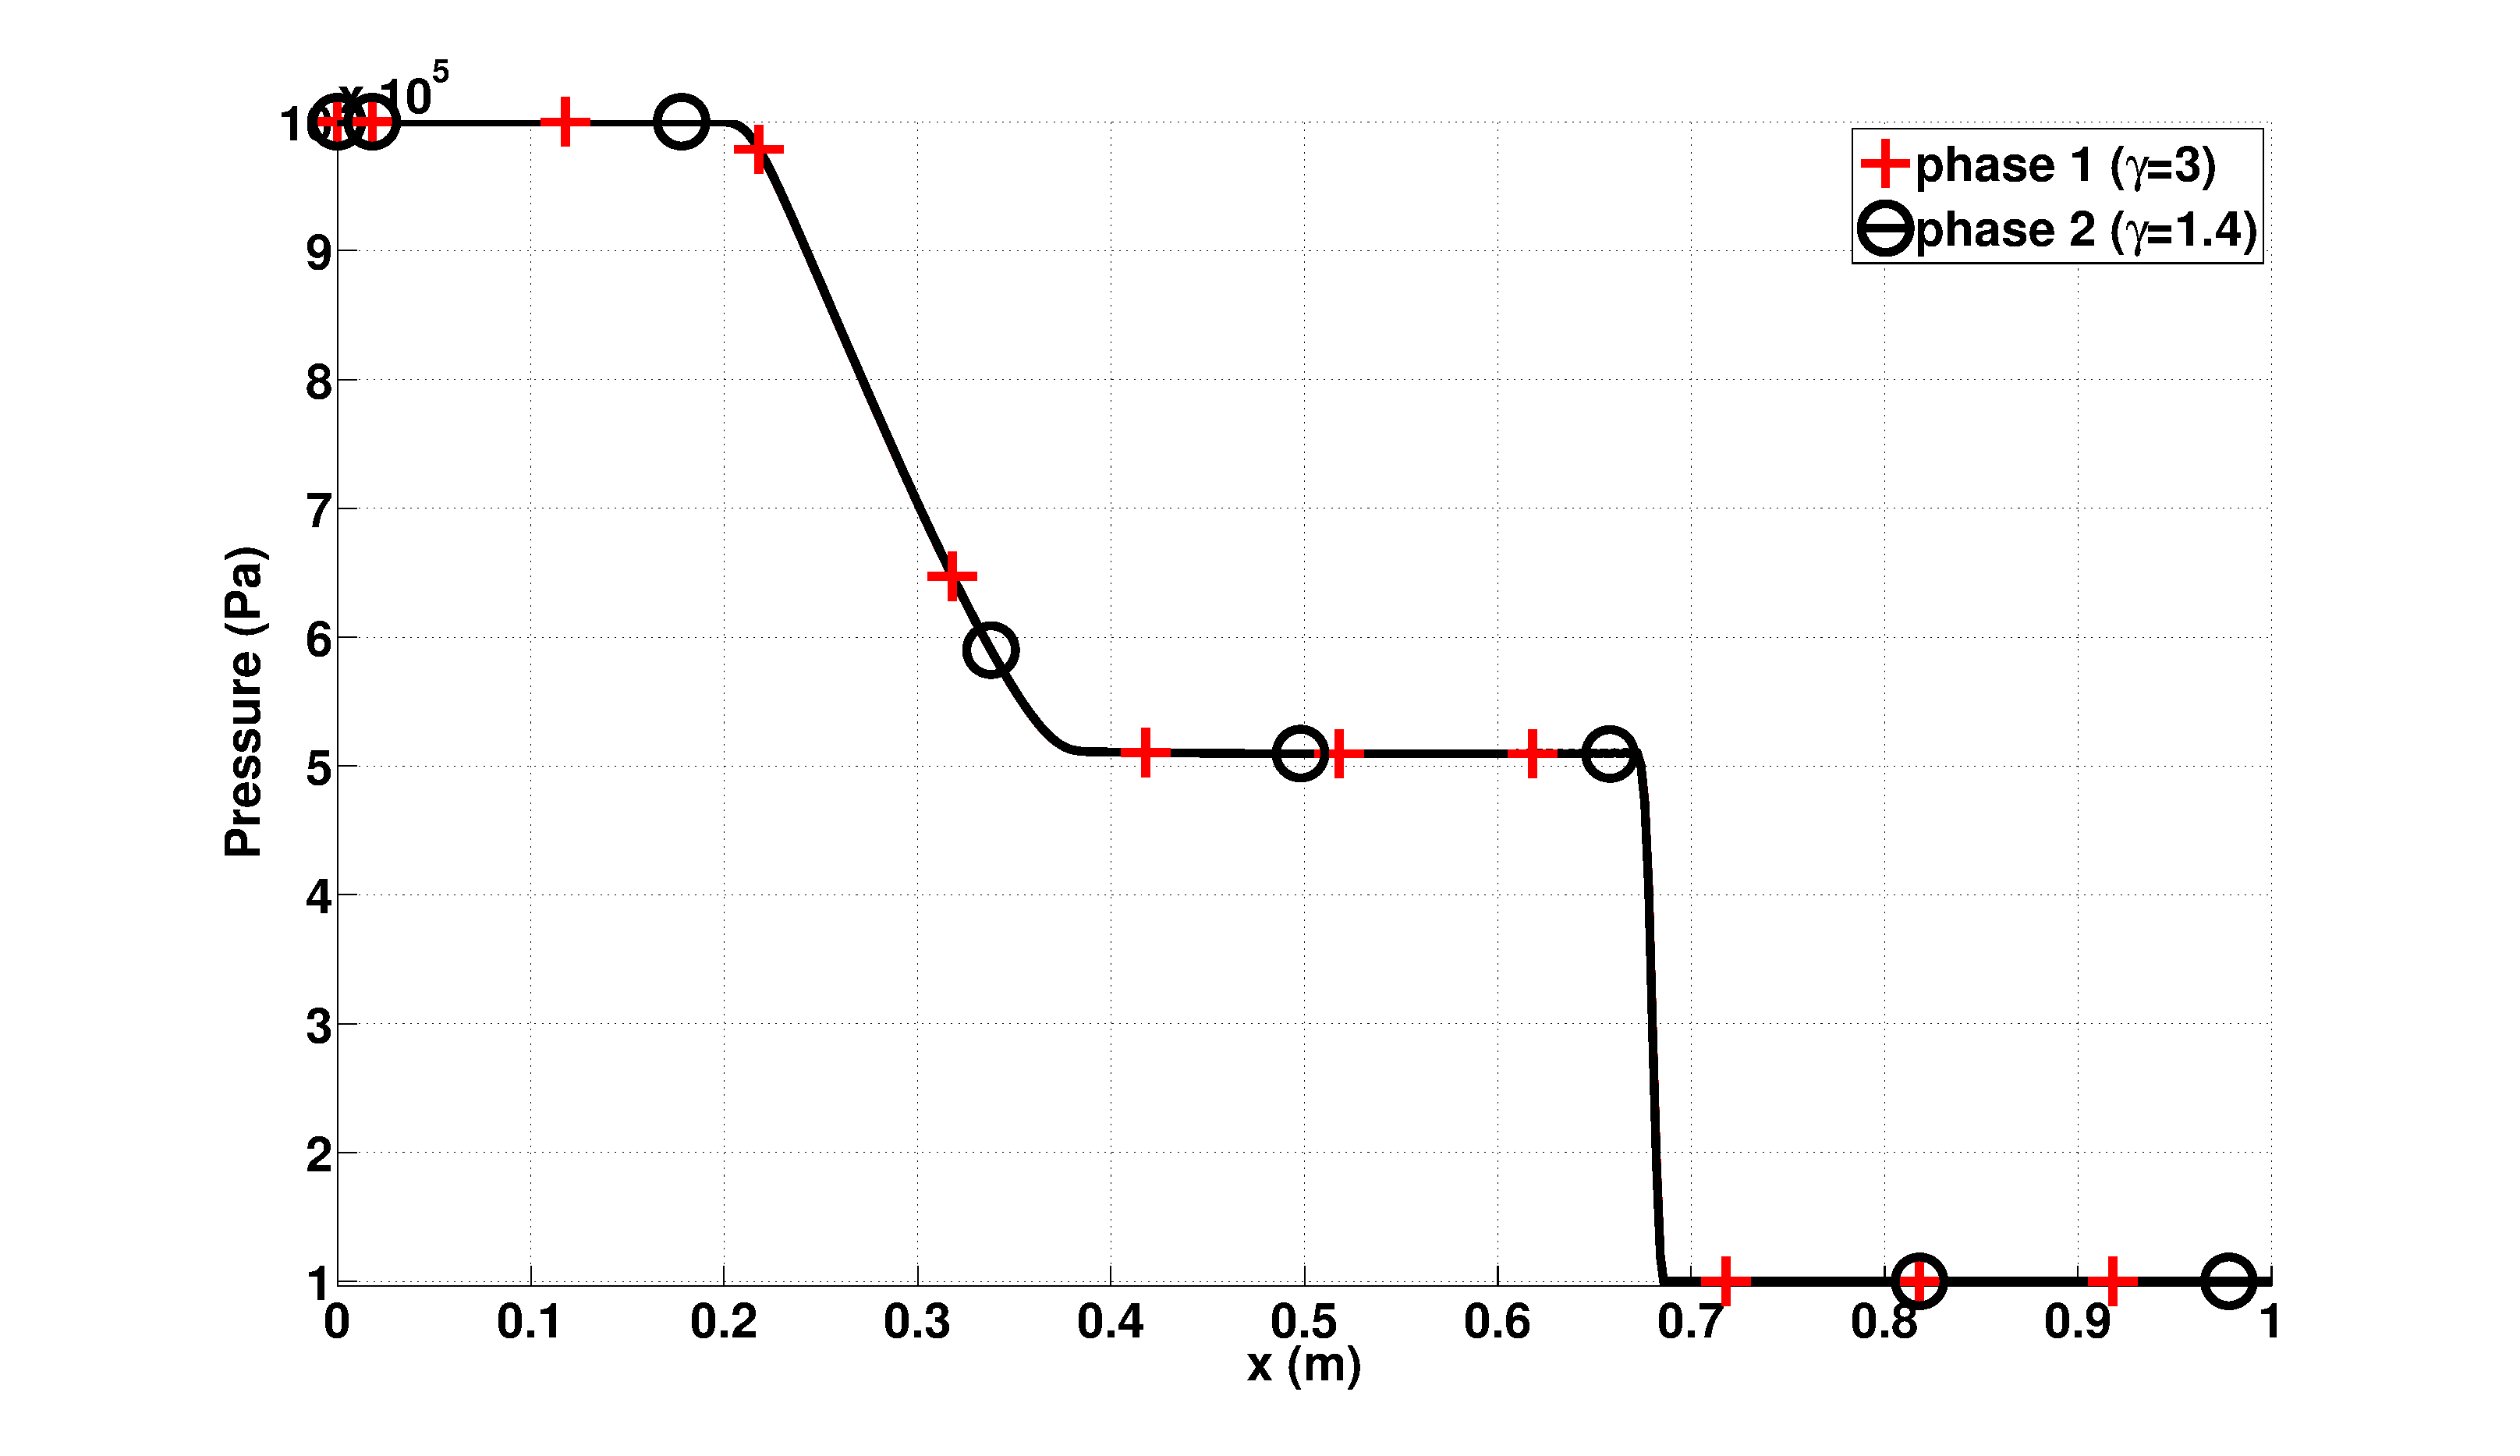
\includegraphics[width=\textwidth]{figures/relaxation_two_phases_pressure.eps}
                \caption{Density}
                \label{fig:inf-rel-density}
        \end{subfigure}
        
        \begin{subfigure}[b]{0.495\textwidth}
                \centering
                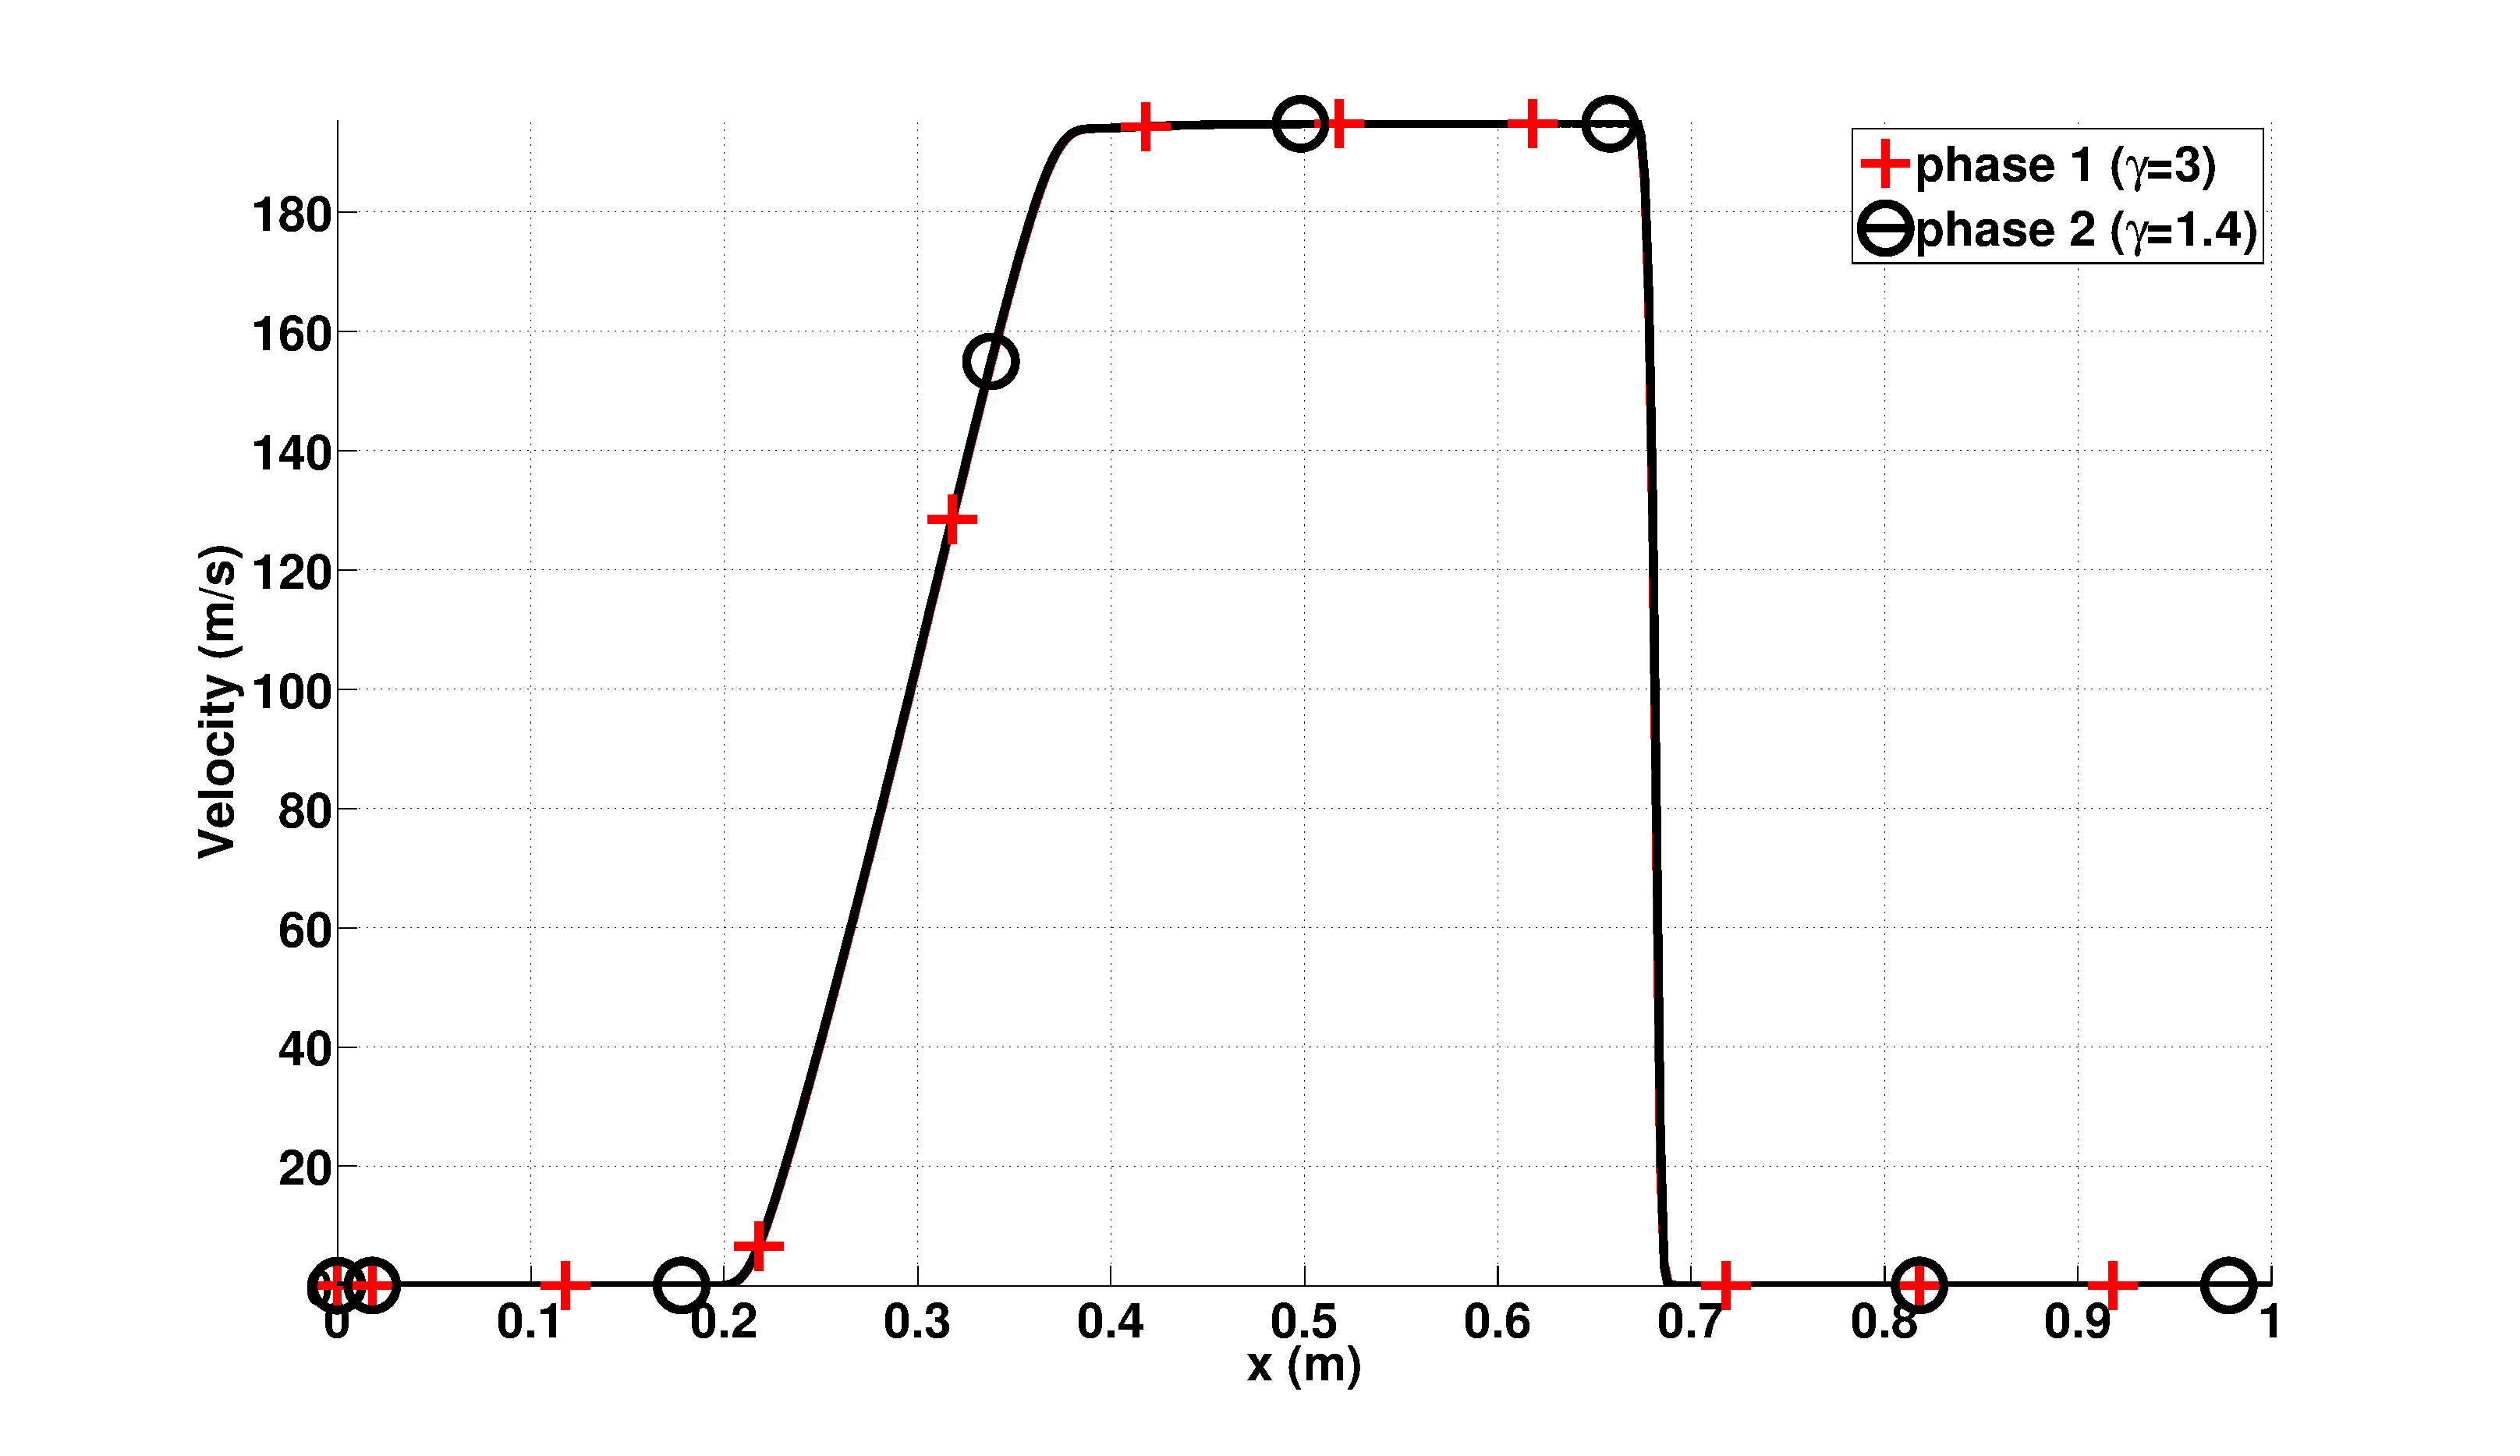
\includegraphics[width=\textwidth]{figures/relaxation_two_phases_velocity.eps}
                \caption{Pressure}
                \label{fig:inf-rel-press}
        \end{subfigure}        
        \begin{subfigure}[b]{0.495\textwidth}
                \centering
                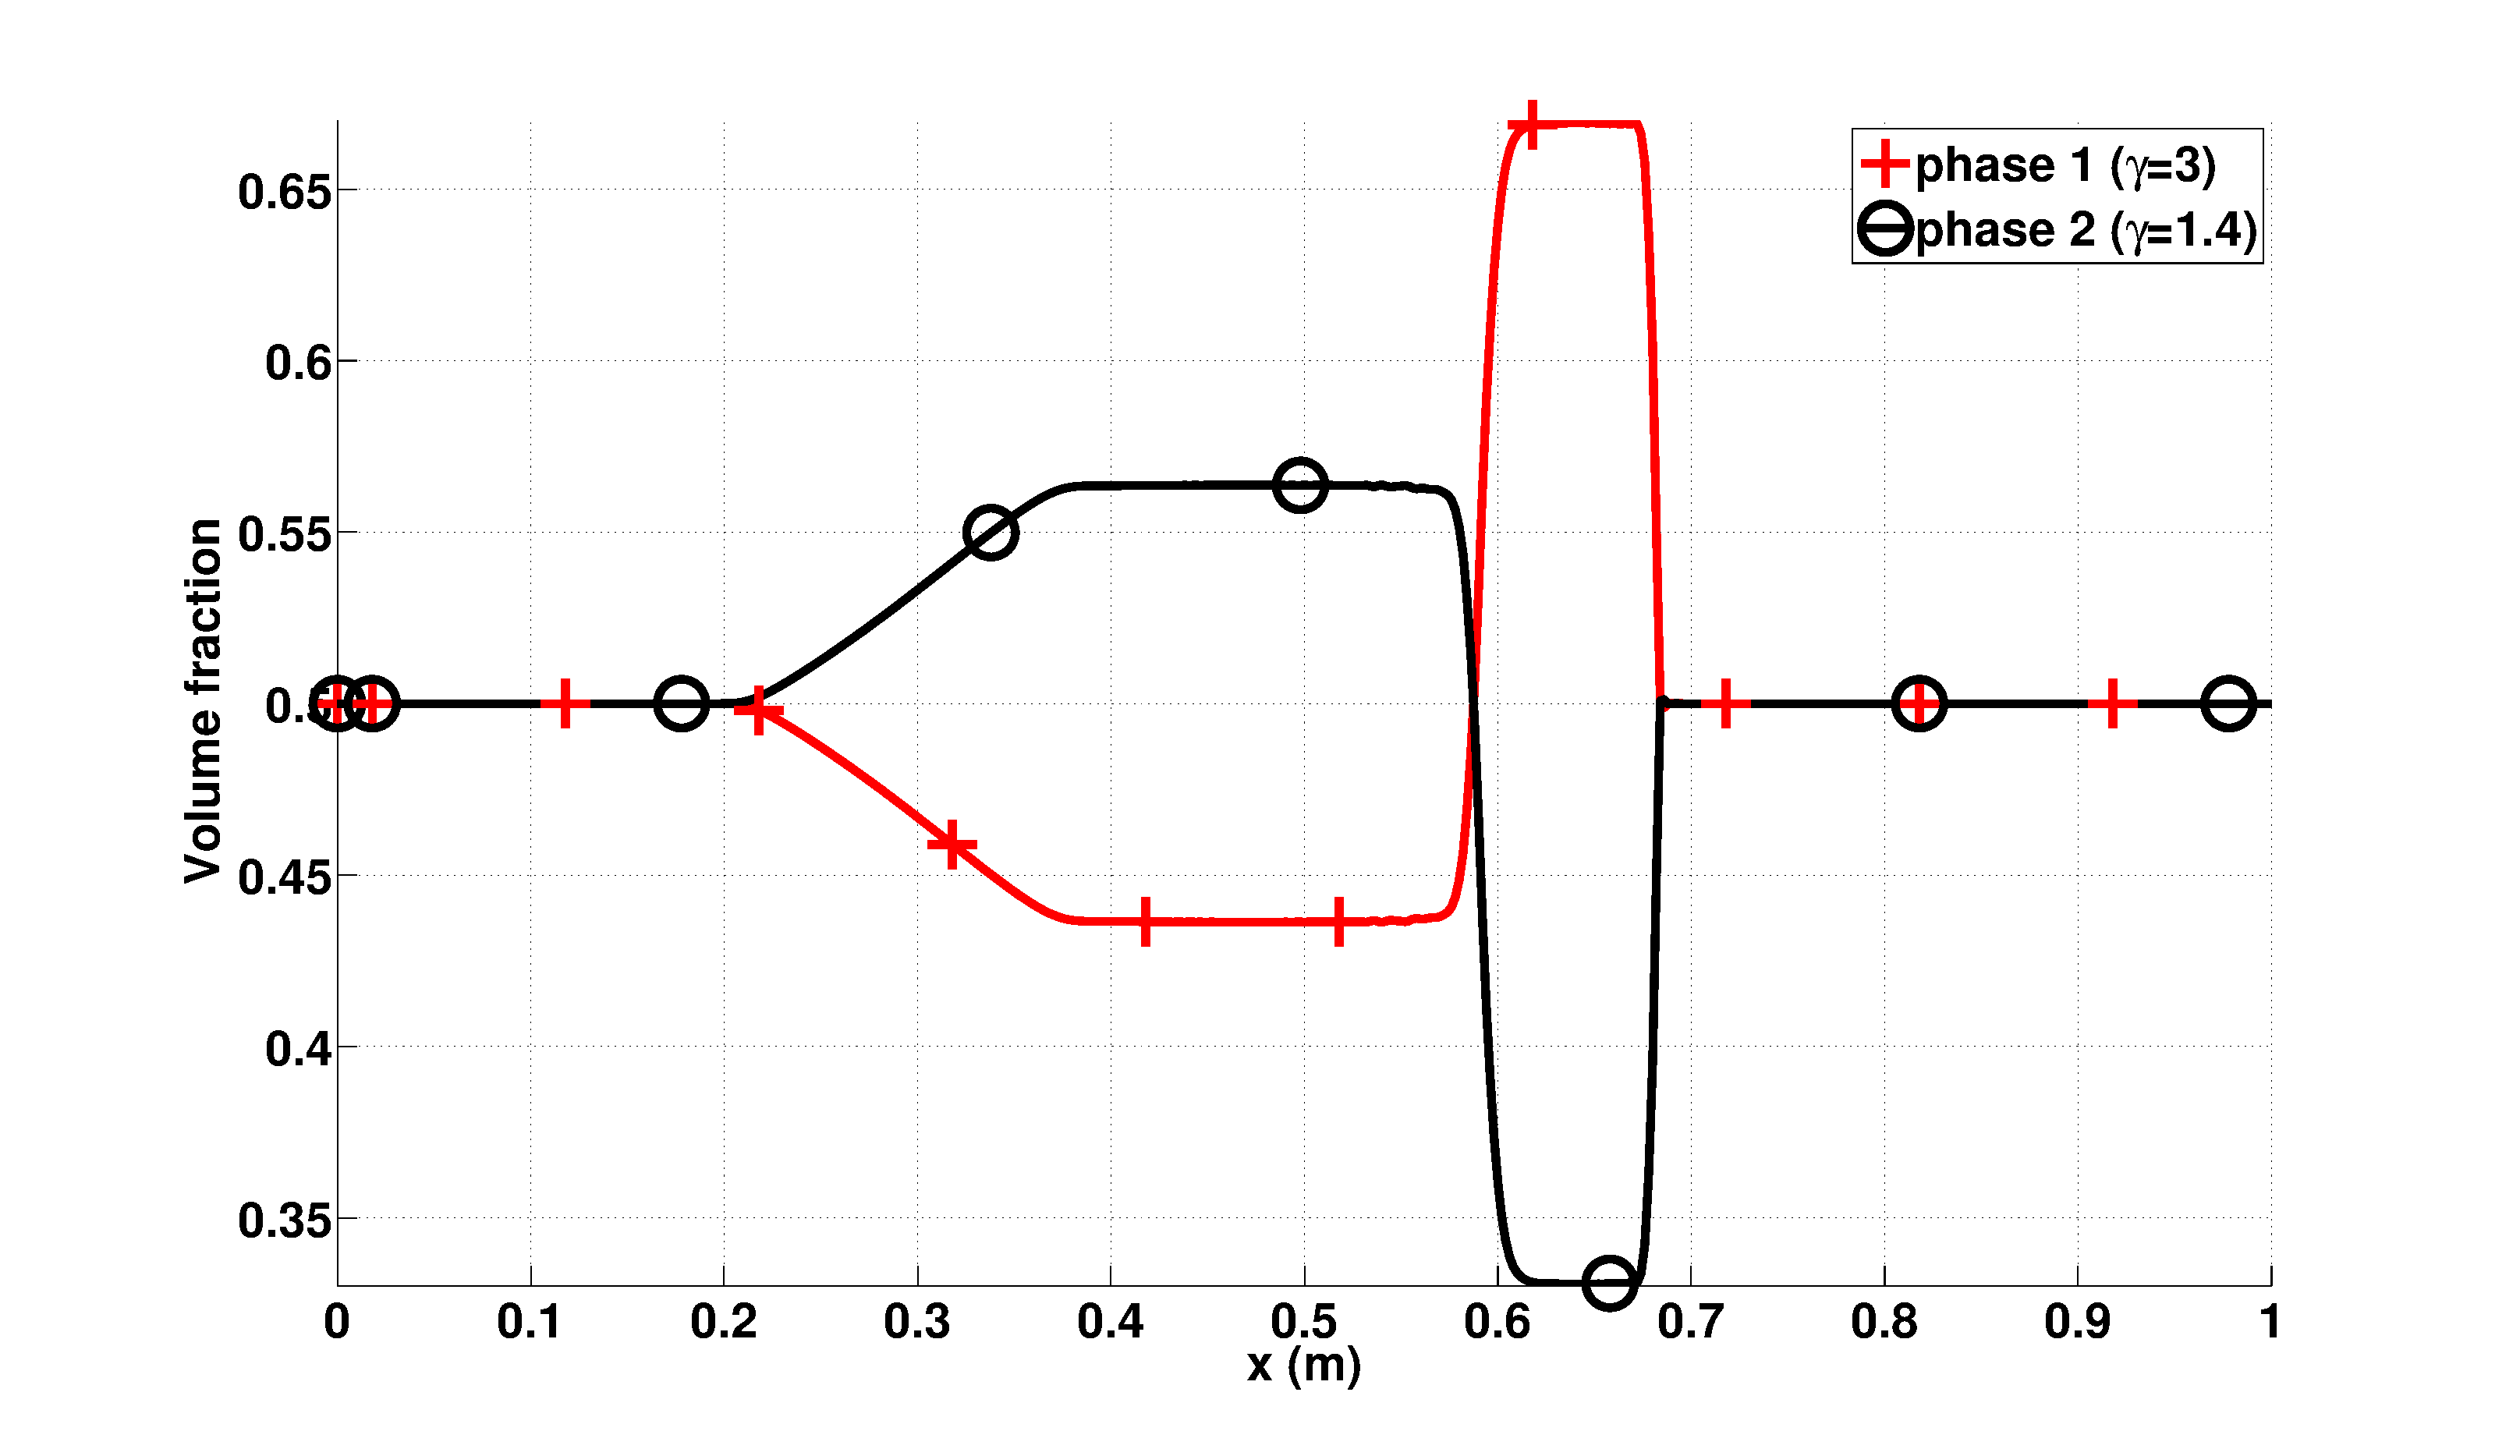
\includegraphics[width=\textwidth]{figures/relaxation_two_phases_volume_fraction.eps}
                \caption{Volume fraction}
                \label{fig:inf-rel-vf}
        \end{subfigure}
        \caption{Numerical solution of a two-phase flow with large relaxation coefficients at $t=305 \ \mu s$.}\label{fig:inf-rel-variables}
\end{figure}
%
As expected, the two fluids have the same pressure and velocity profiles as shown in \fig{fig:inf-rel-press} and \fig{fig:inf-rel-vel}, respectively. The shock is well resolved and does not display any instability. The main difference with the numerical results obtained in \sct{sec:shock-tube-two-indep-fluids} lies in the volume fraction profiles that are no longer uniform but display a shock wave around $x=0.7$ $m$ as shown in \fig{fig:inf-rel-vf}. Note also that the phasic density profiles given in \fig{fig:inf-rel-density} are not equal but experience the same variations : a shock and a contact discontinuity around $x=0.7 \ m$ and $x = 0.6 \ m$, respectively. 
%
\begin{figure}[H]
        \centering
        \begin{subfigure}[b]{0.495\textwidth}
                \centering
                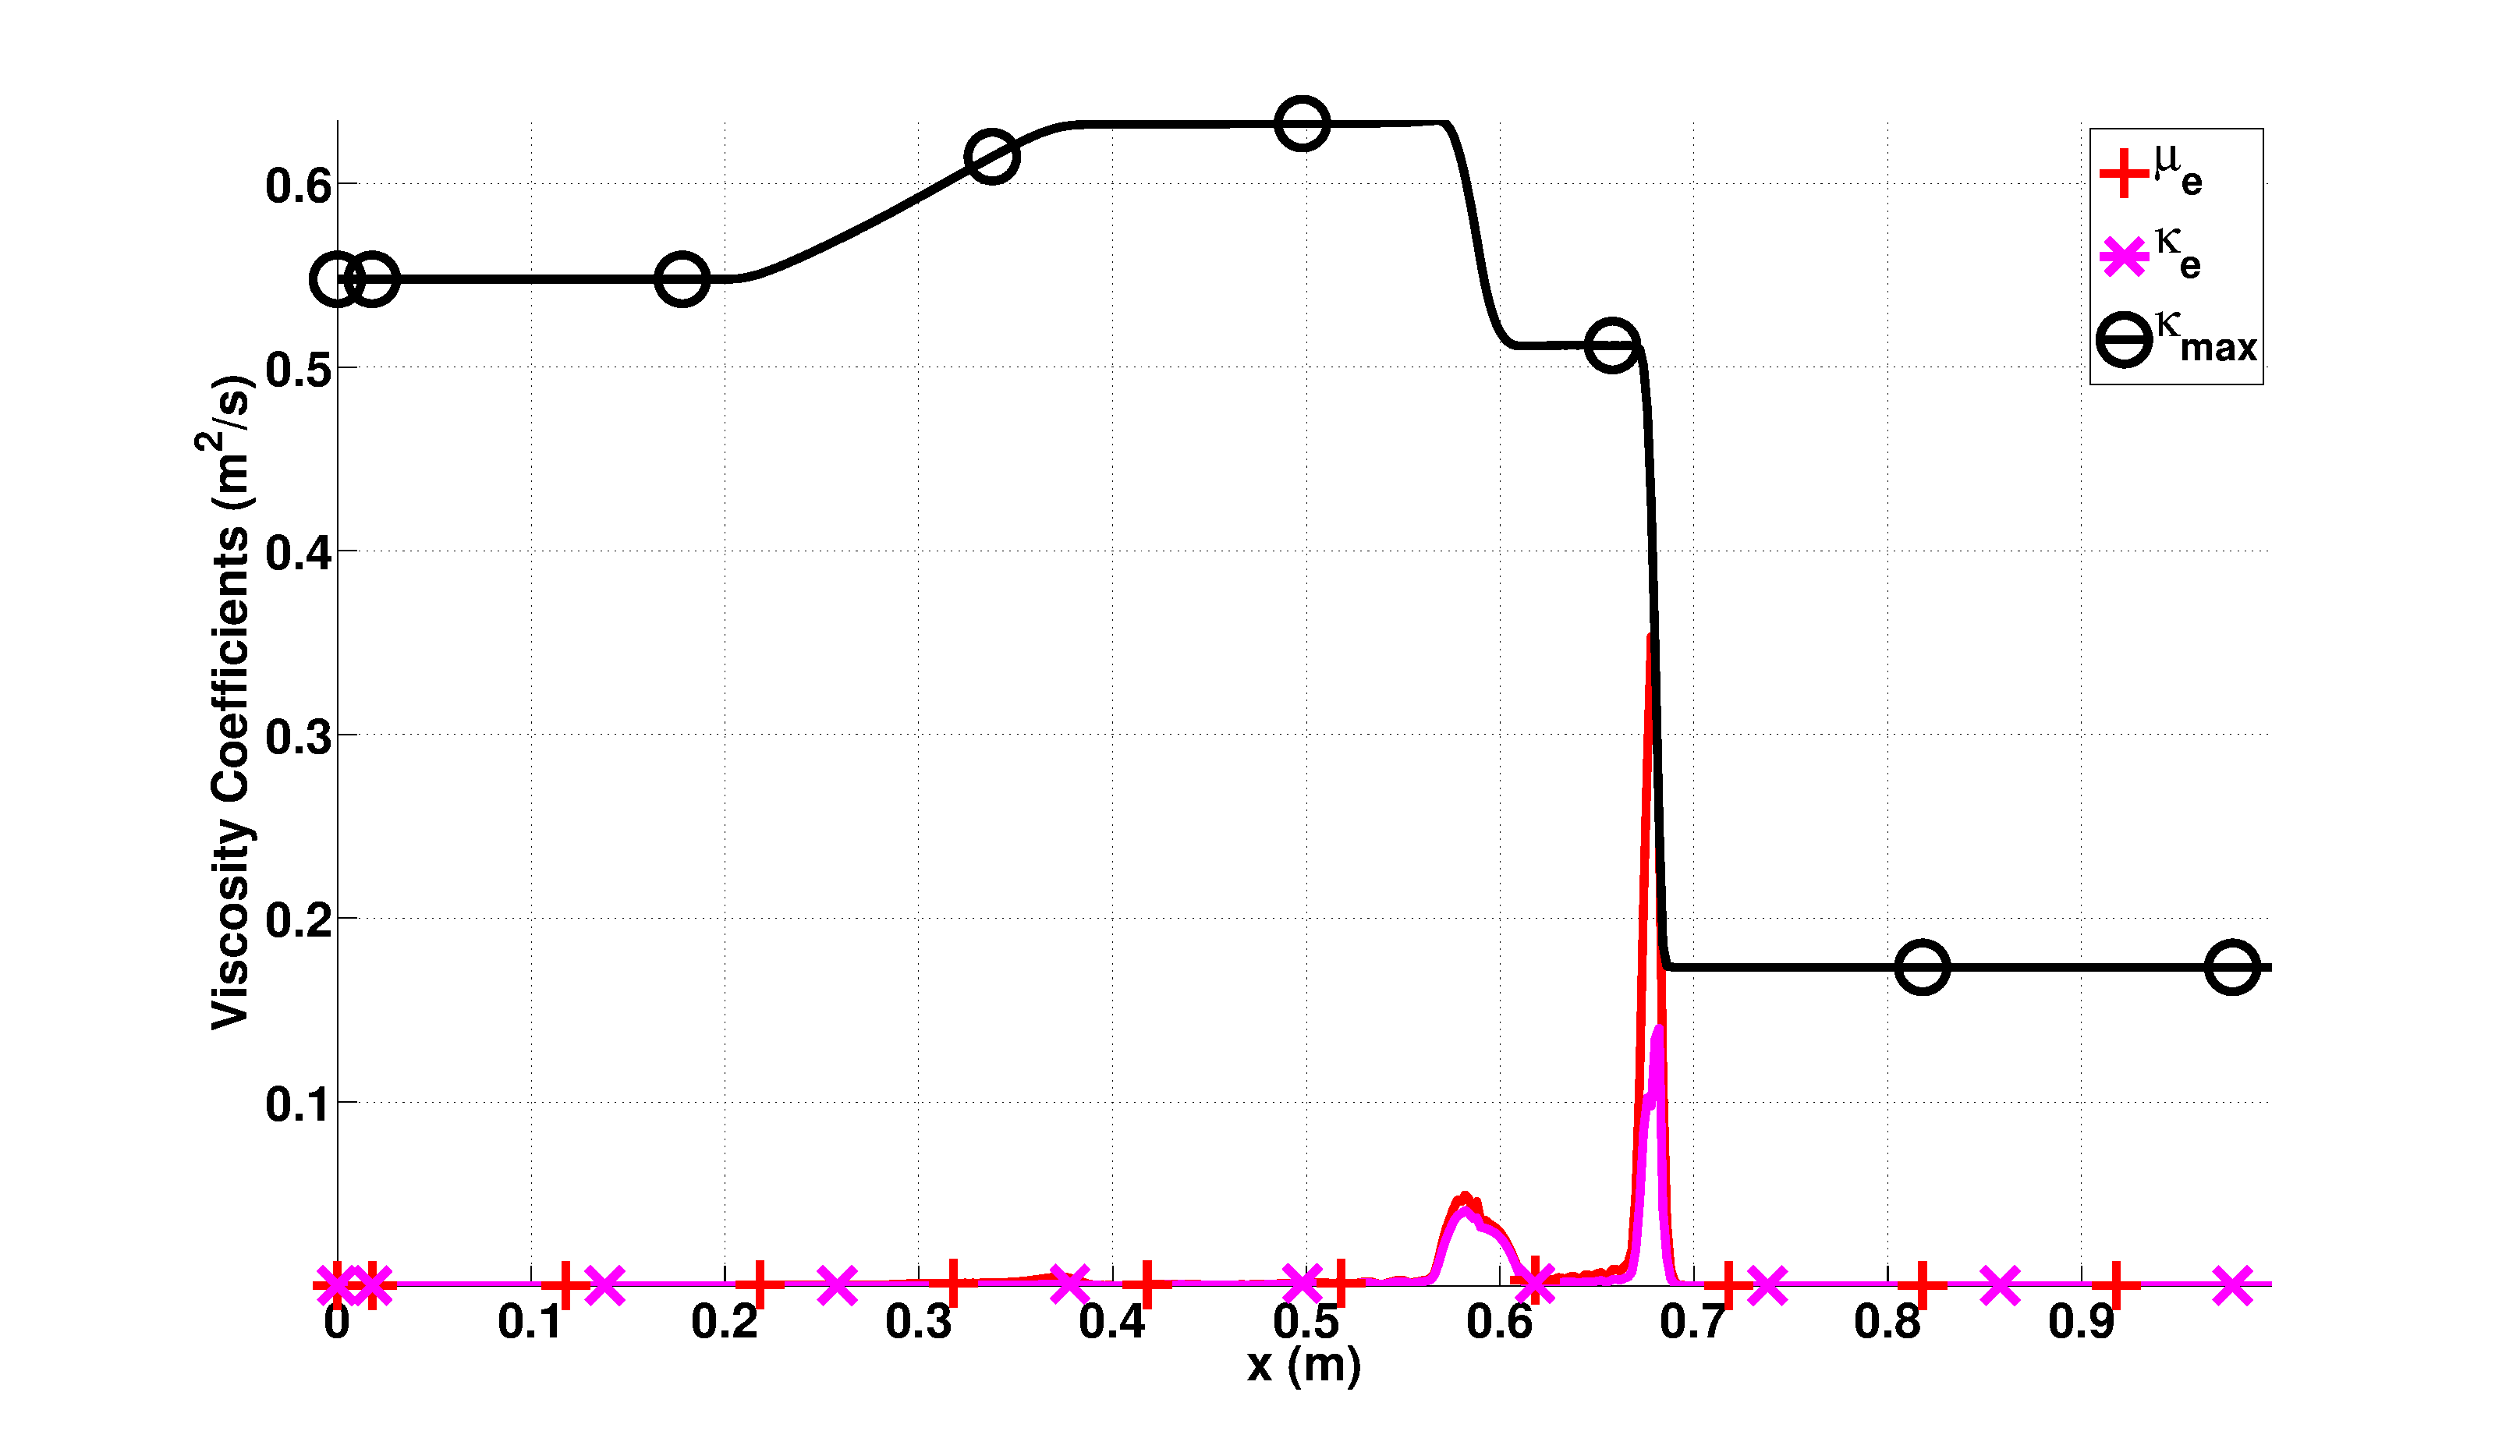
\includegraphics[width=\textwidth]{figures/relaxation_phase_1_viscosity_kappa_mu.eps}
                \caption{Viscosity coefficients for phase 1.}
                \label{fig:inf-rel-visc-coeff-phase-1}
        \end{subfigure}%
        \begin{subfigure}[b]{0.495\textwidth}
                \centering
                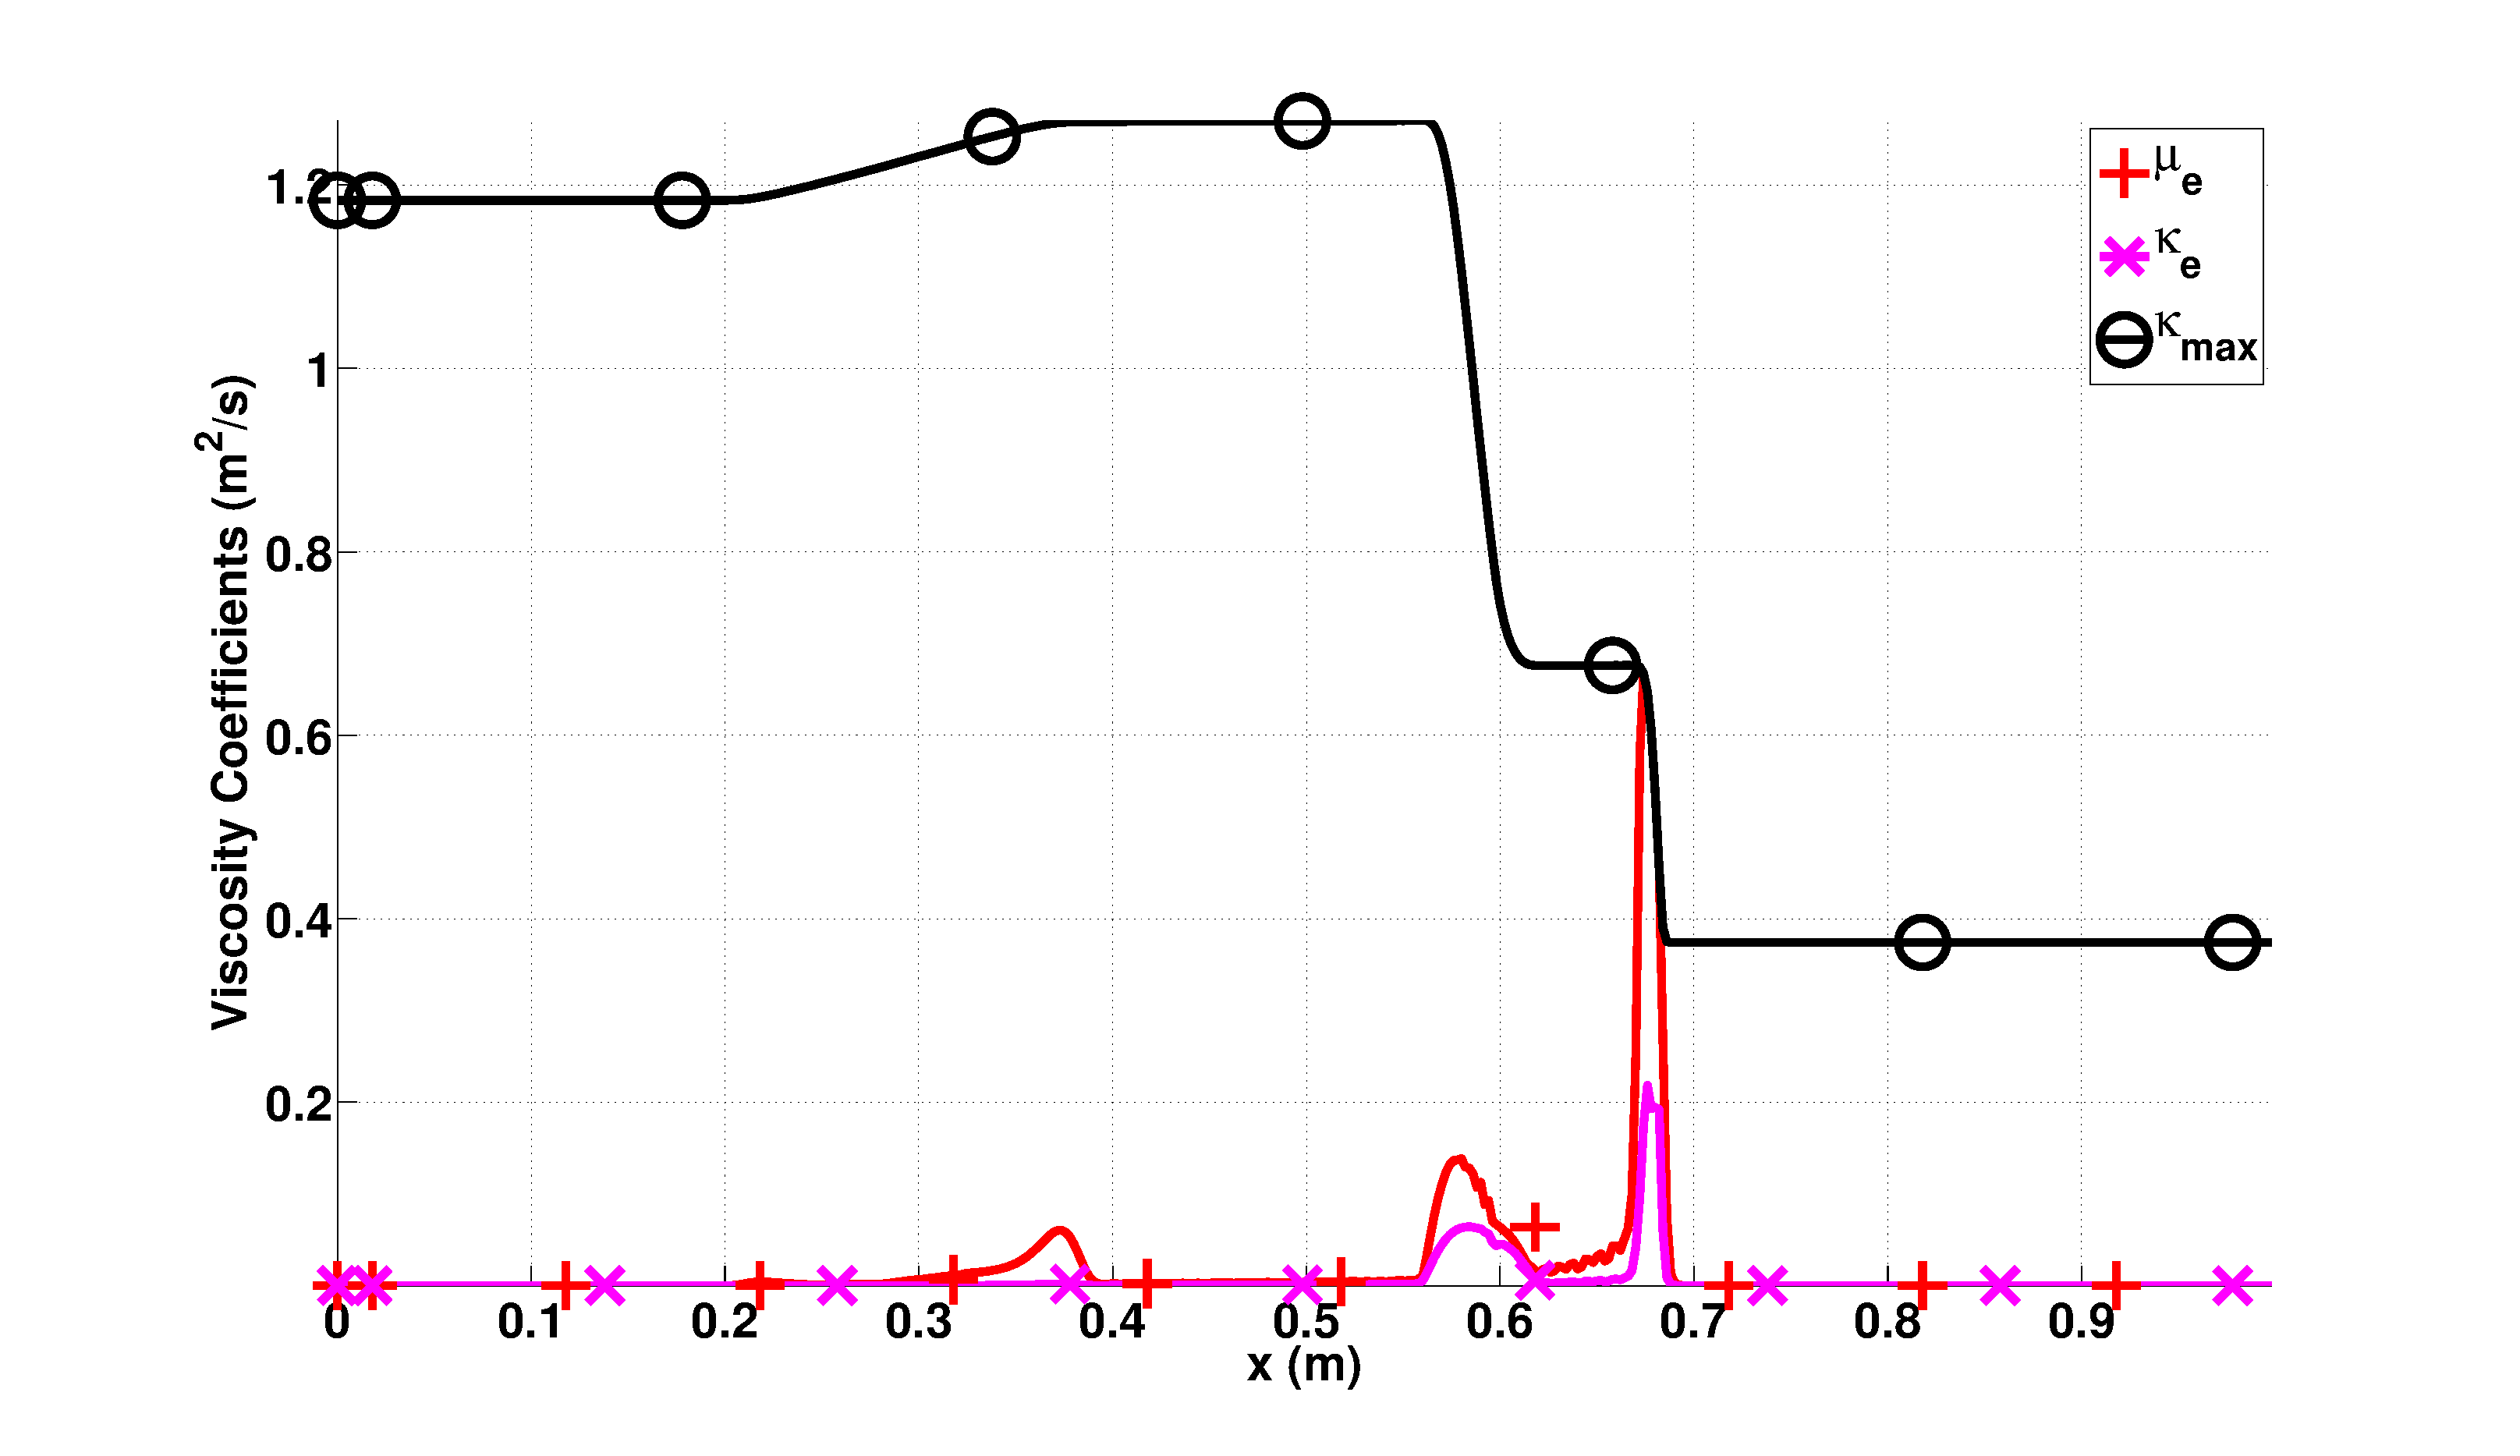
\includegraphics[width=\textwidth]{figures/relaxation_phase_2_viscosity_kappa_mu.eps}
                \caption{Viscosity coefficients for phase 2}
                \label{fig:inf-rel-visc-coeff-phase-2}
        \end{subfigure}
        
        \begin{subfigure}[b]{0.495\textwidth}
                \centering
                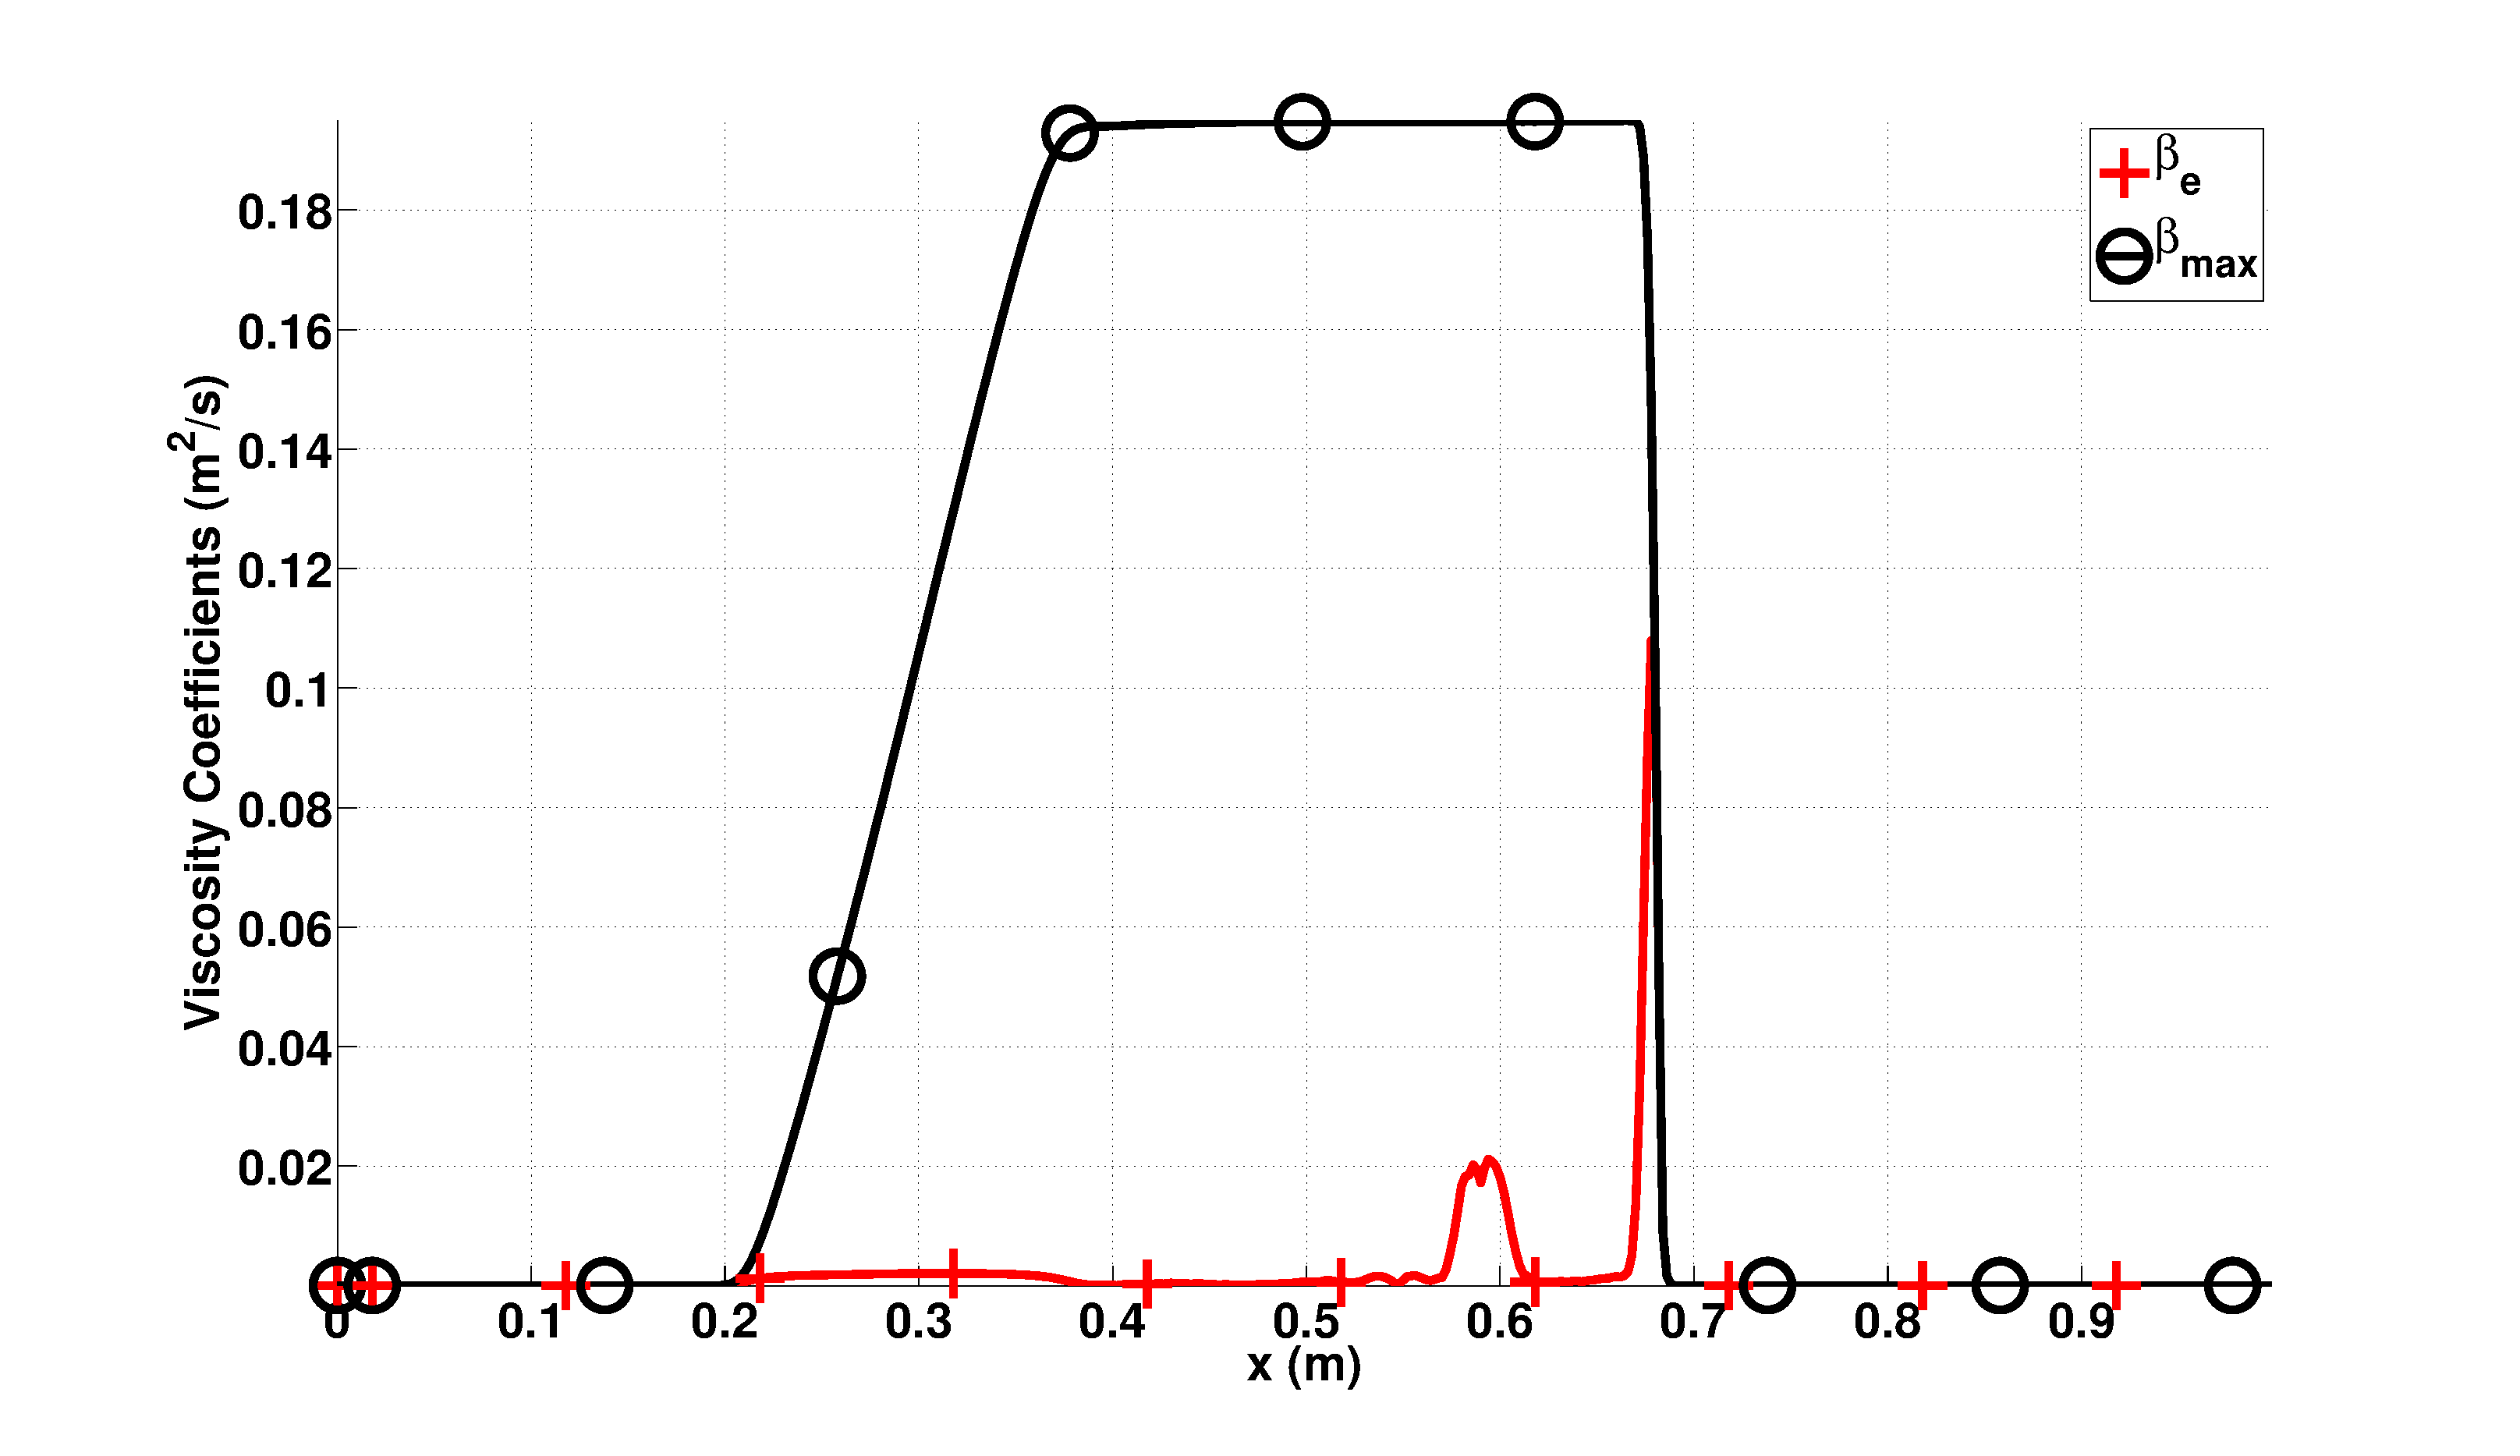
\includegraphics[width=\textwidth]{figures/relaxation_phase_1_beta.eps}
                \caption{Viscosity coefficients for the volume fraction equation of phase 1.}
                \label{fig:inf-rel-beta}
        \end{subfigure}        
        \caption{Viscosity coefficients profiles for a two-phase flow with large relaxation coefficients at $t=305 \ \mu s$.}\label{fig:inf-rel-visc-coeff}
\end{figure}
%
The variations of the phasic viscosity coefficients are consistent with the position of the shock and contact discontinuity previously observed in \fig{fig:inf-rel-variables}. The phasic viscosity coefficients are peaked in the vicinity of the shock and saturate to the first-order viscosity coefficients. A small peak is also observed in the contact discontinuity.\\
\tcb{I want to add an exact solution to the plots obtained from Ray's code. I think if Ray's solution is fine enough, we can probably do a convergence test.}
%
%%%%%%%%%%%%%%%%%%%%%%%%%%%%%%%%%%%%%
\subsubsection{Two independent fluids in a 1-D converging-diverging nozzle}\label{sec:nozzle-two-indep-fluids}
%%%%%%%%%%%%%%%%%%%%%%%%%%%%%%%%%%%%%
%
A simulation for a two-phase flow through a 1-D converging-diverging nozzle is performed. The variable area function is given by 
$A(x) = 1 + \tfrac{1}{2} \cos(2 \pi x / L)$ with length L $=1 \ m$.  At the inlet, the stagnation pressure and temperature are set 
to $P_0 = 1 \ MPa$ and $T_0 = 453 \ K$, respectively. At the outlet, only the static pressure is specified: $P_s = 0.5 \ MPa$. 
Initially, the liquid is at rest, the temperature is uniform and equal to the stagnation temperature and the pressure 
linearly decreases from the stagnation pressure inlet value to the static pressure outlet value. 
The stiffened gas equation of state is used to model the liquid water and vapor phases with the parameters provided in \tbl{tbl:stff_gas_eos-sect4}.
Because of the low pressure difference between the inlet and the outlet, the smooth initial conditions, 
and the large value of $P_\infty$ in \eqt{eq:generic-form}, the flow of the liquid water remains subsonic and thus displays no shock. The vapor phase, however, experiences a shock at steady state as the compressive effects are dominant (the liquid to gas density ratio is about $1,000$). A detailed 
derivation of the exact steady-state solution when considering each phase independently can be found in \cite{nozzle_exact}. An uniform mesh of 
200 cells was used to obtain the numerical solution and the time step size was computed using an initial CFL number of one (the CFL is increased as the numerical solution approaches steady state).
This test was first introduced by Saurel et al. in \cite{SEM} and allows to assess the behavior of the numerical method in the low-Mach asymptotic limit.
The initial conditions are computed from the boundary conditions by assuming the two fluids at rest and linearly interpolating the pressure and temperature between the boundary values.
%
\begin{table}[H]
\begin{center}
\caption{ Stiffened Gas Equation of State (SGEOS) parameters for steam and liquid water.}
\label{tbl:stff_gas_eos-sect4}
\begin{tabular}{|c|c|c|c|c|}
 \hline
\text{fluid}                           & $\gamma$ & $C_v$ $(J.kg^{-1}.K^{-1})$ & $P_\infty$ $(Pa)$ & $q$ $(J.kg^{-1})$ \\  \hline \hline
liquid water & 2.35     & 1816                       & $10^9$            & $-1167\ 10^3$     \\  \hline
steam          & 1.43     & 1040                       & 0                 & $ 2030\ 10^3$     \\  \hline
\end{tabular}
\end{center}
\end{table}
%
The geometry is discretized with an uniform mesh of 200 cells and run until steady state. Because each phase is independent of each other, the same numerical solution could be obtained by solving the $1$-D Euler equations with variable area. Steady-state numerical solutions are presented in \fig{fig:nozzle-indep-variables} and plotted along the exact solution. The phasic viscosity coefficient profiles are given in \fig{fig:nozzle-indep-visc-coeff} for both phases.
%
\begin{figure}[H]
        \centering
        \begin{subfigure}[b]{0.495\textwidth}
                \centering
                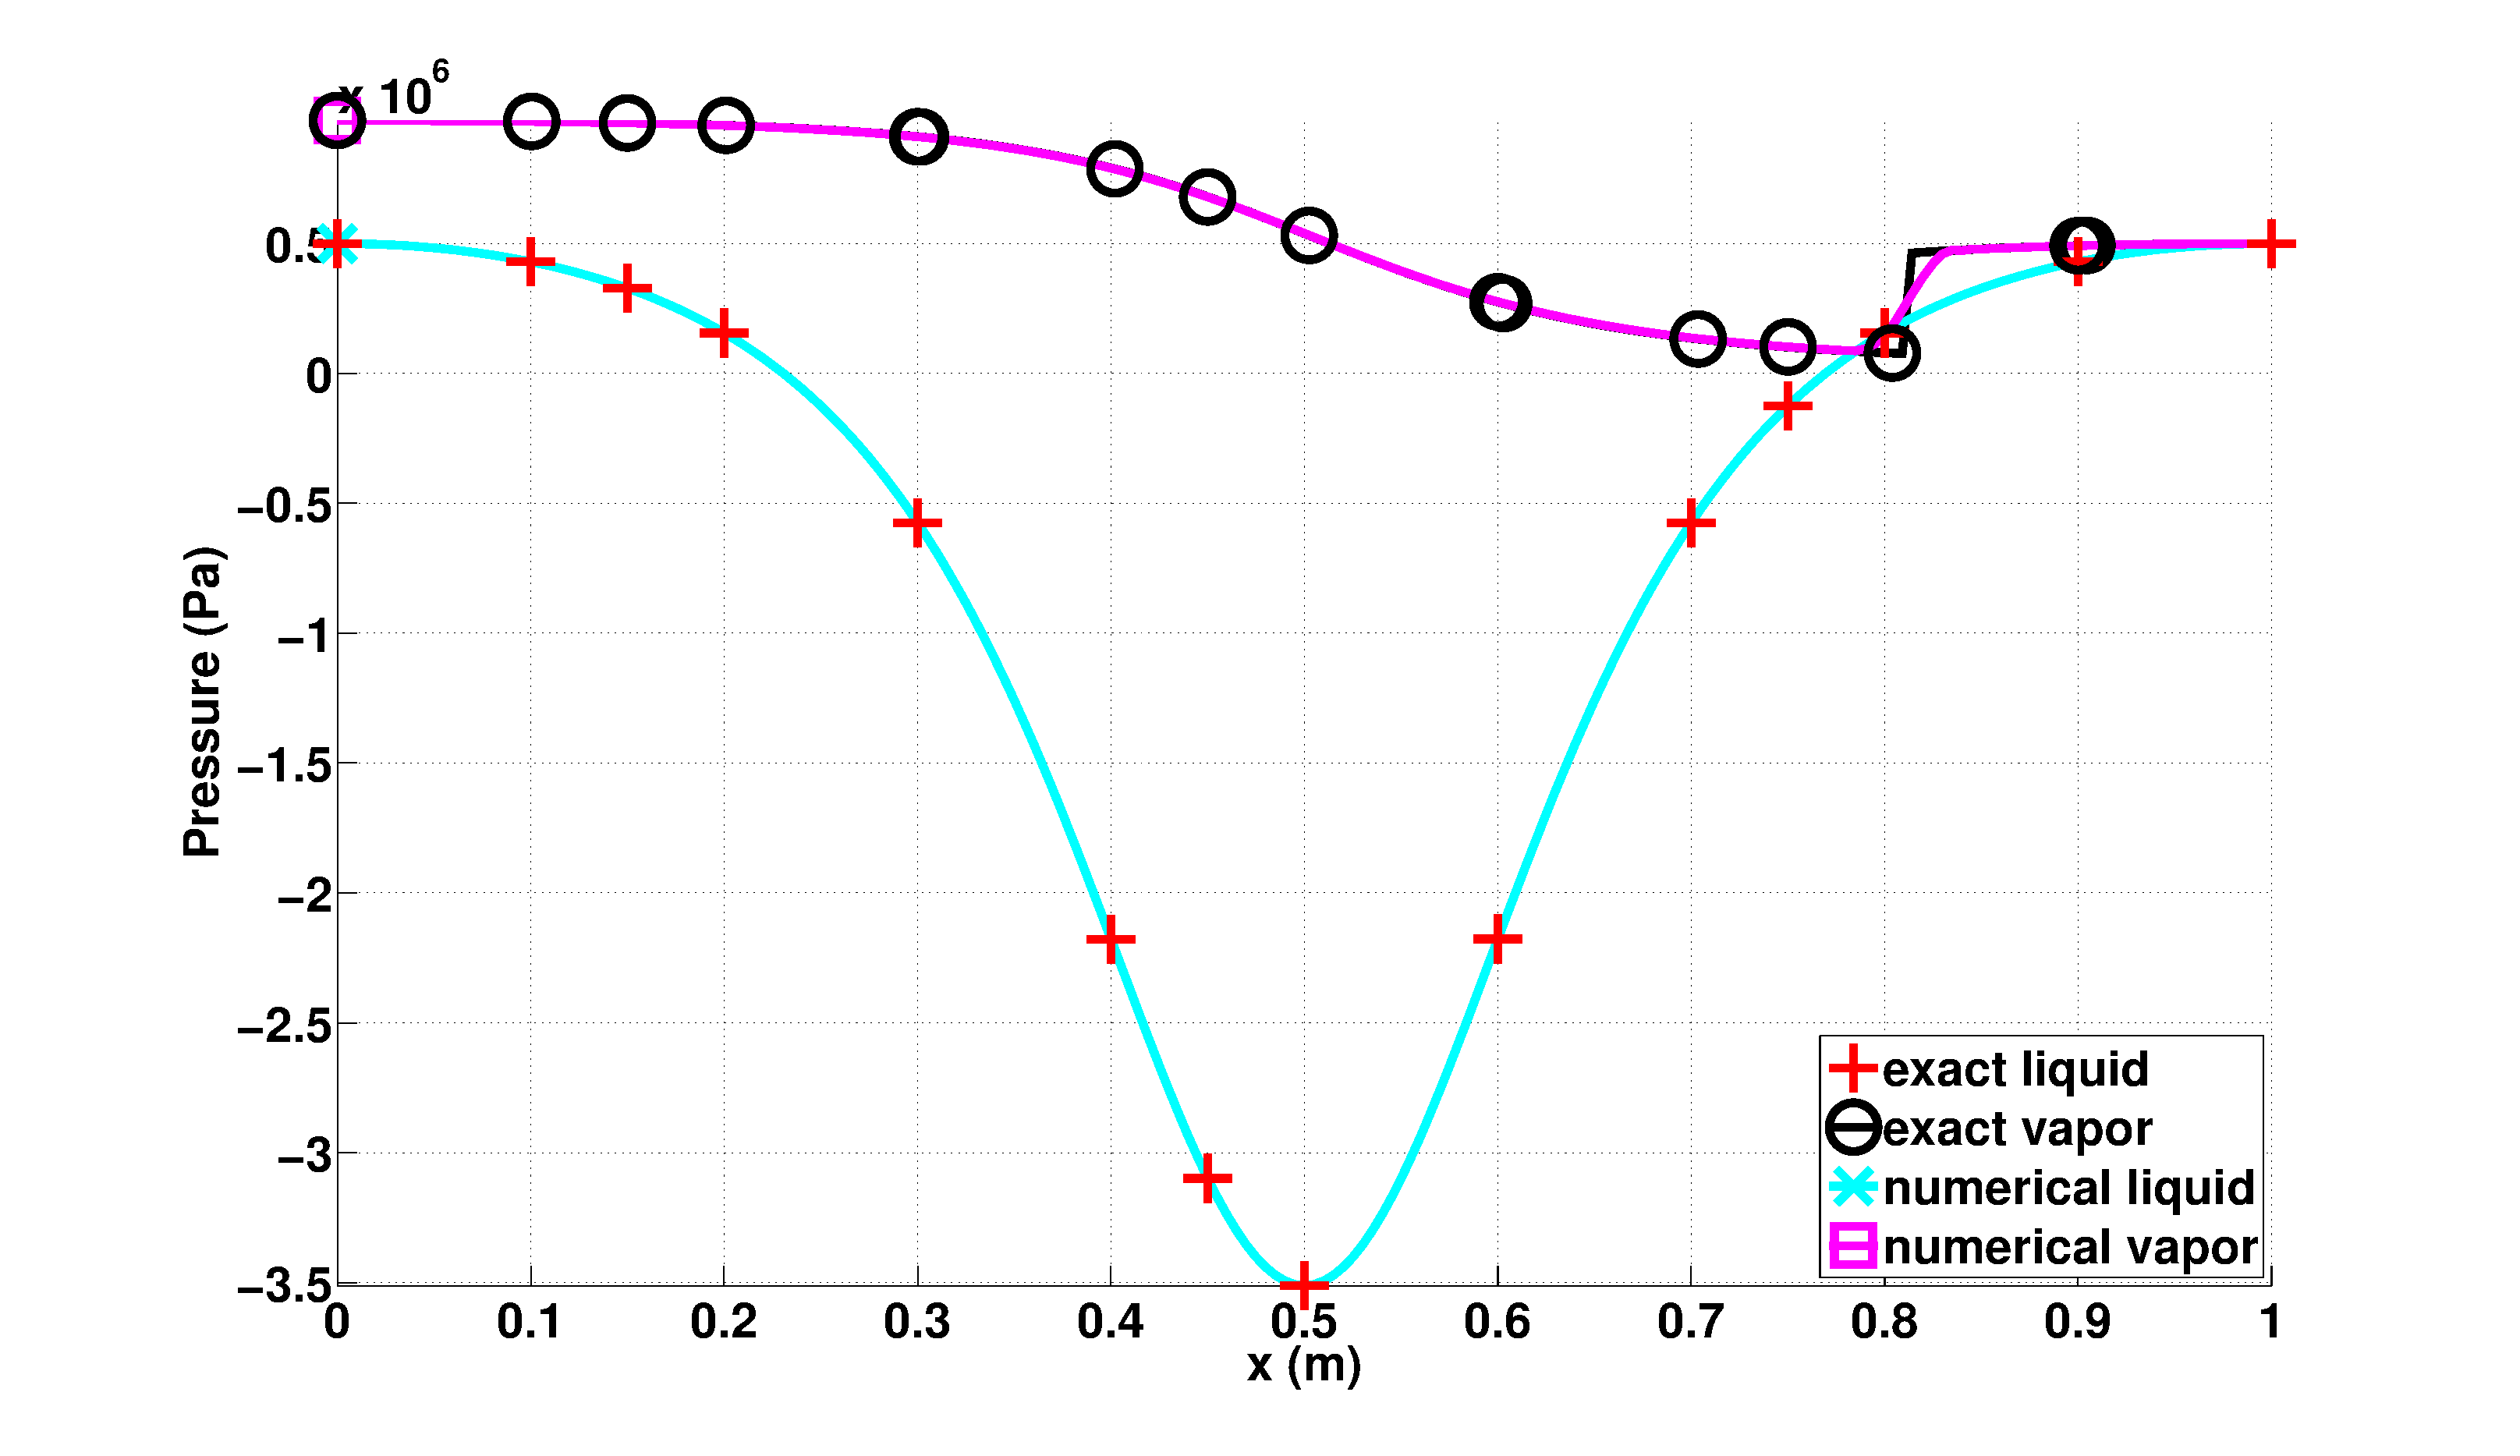
\includegraphics[width=\textwidth]{figures/nozzle-indep-phase_two_phases_pressure.eps}
                \caption{Pressure}
                \label{fig:nozzle-indep-press}
        \end{subfigure}        
        \begin{subfigure}[b]{0.495\textwidth}
                \centering
                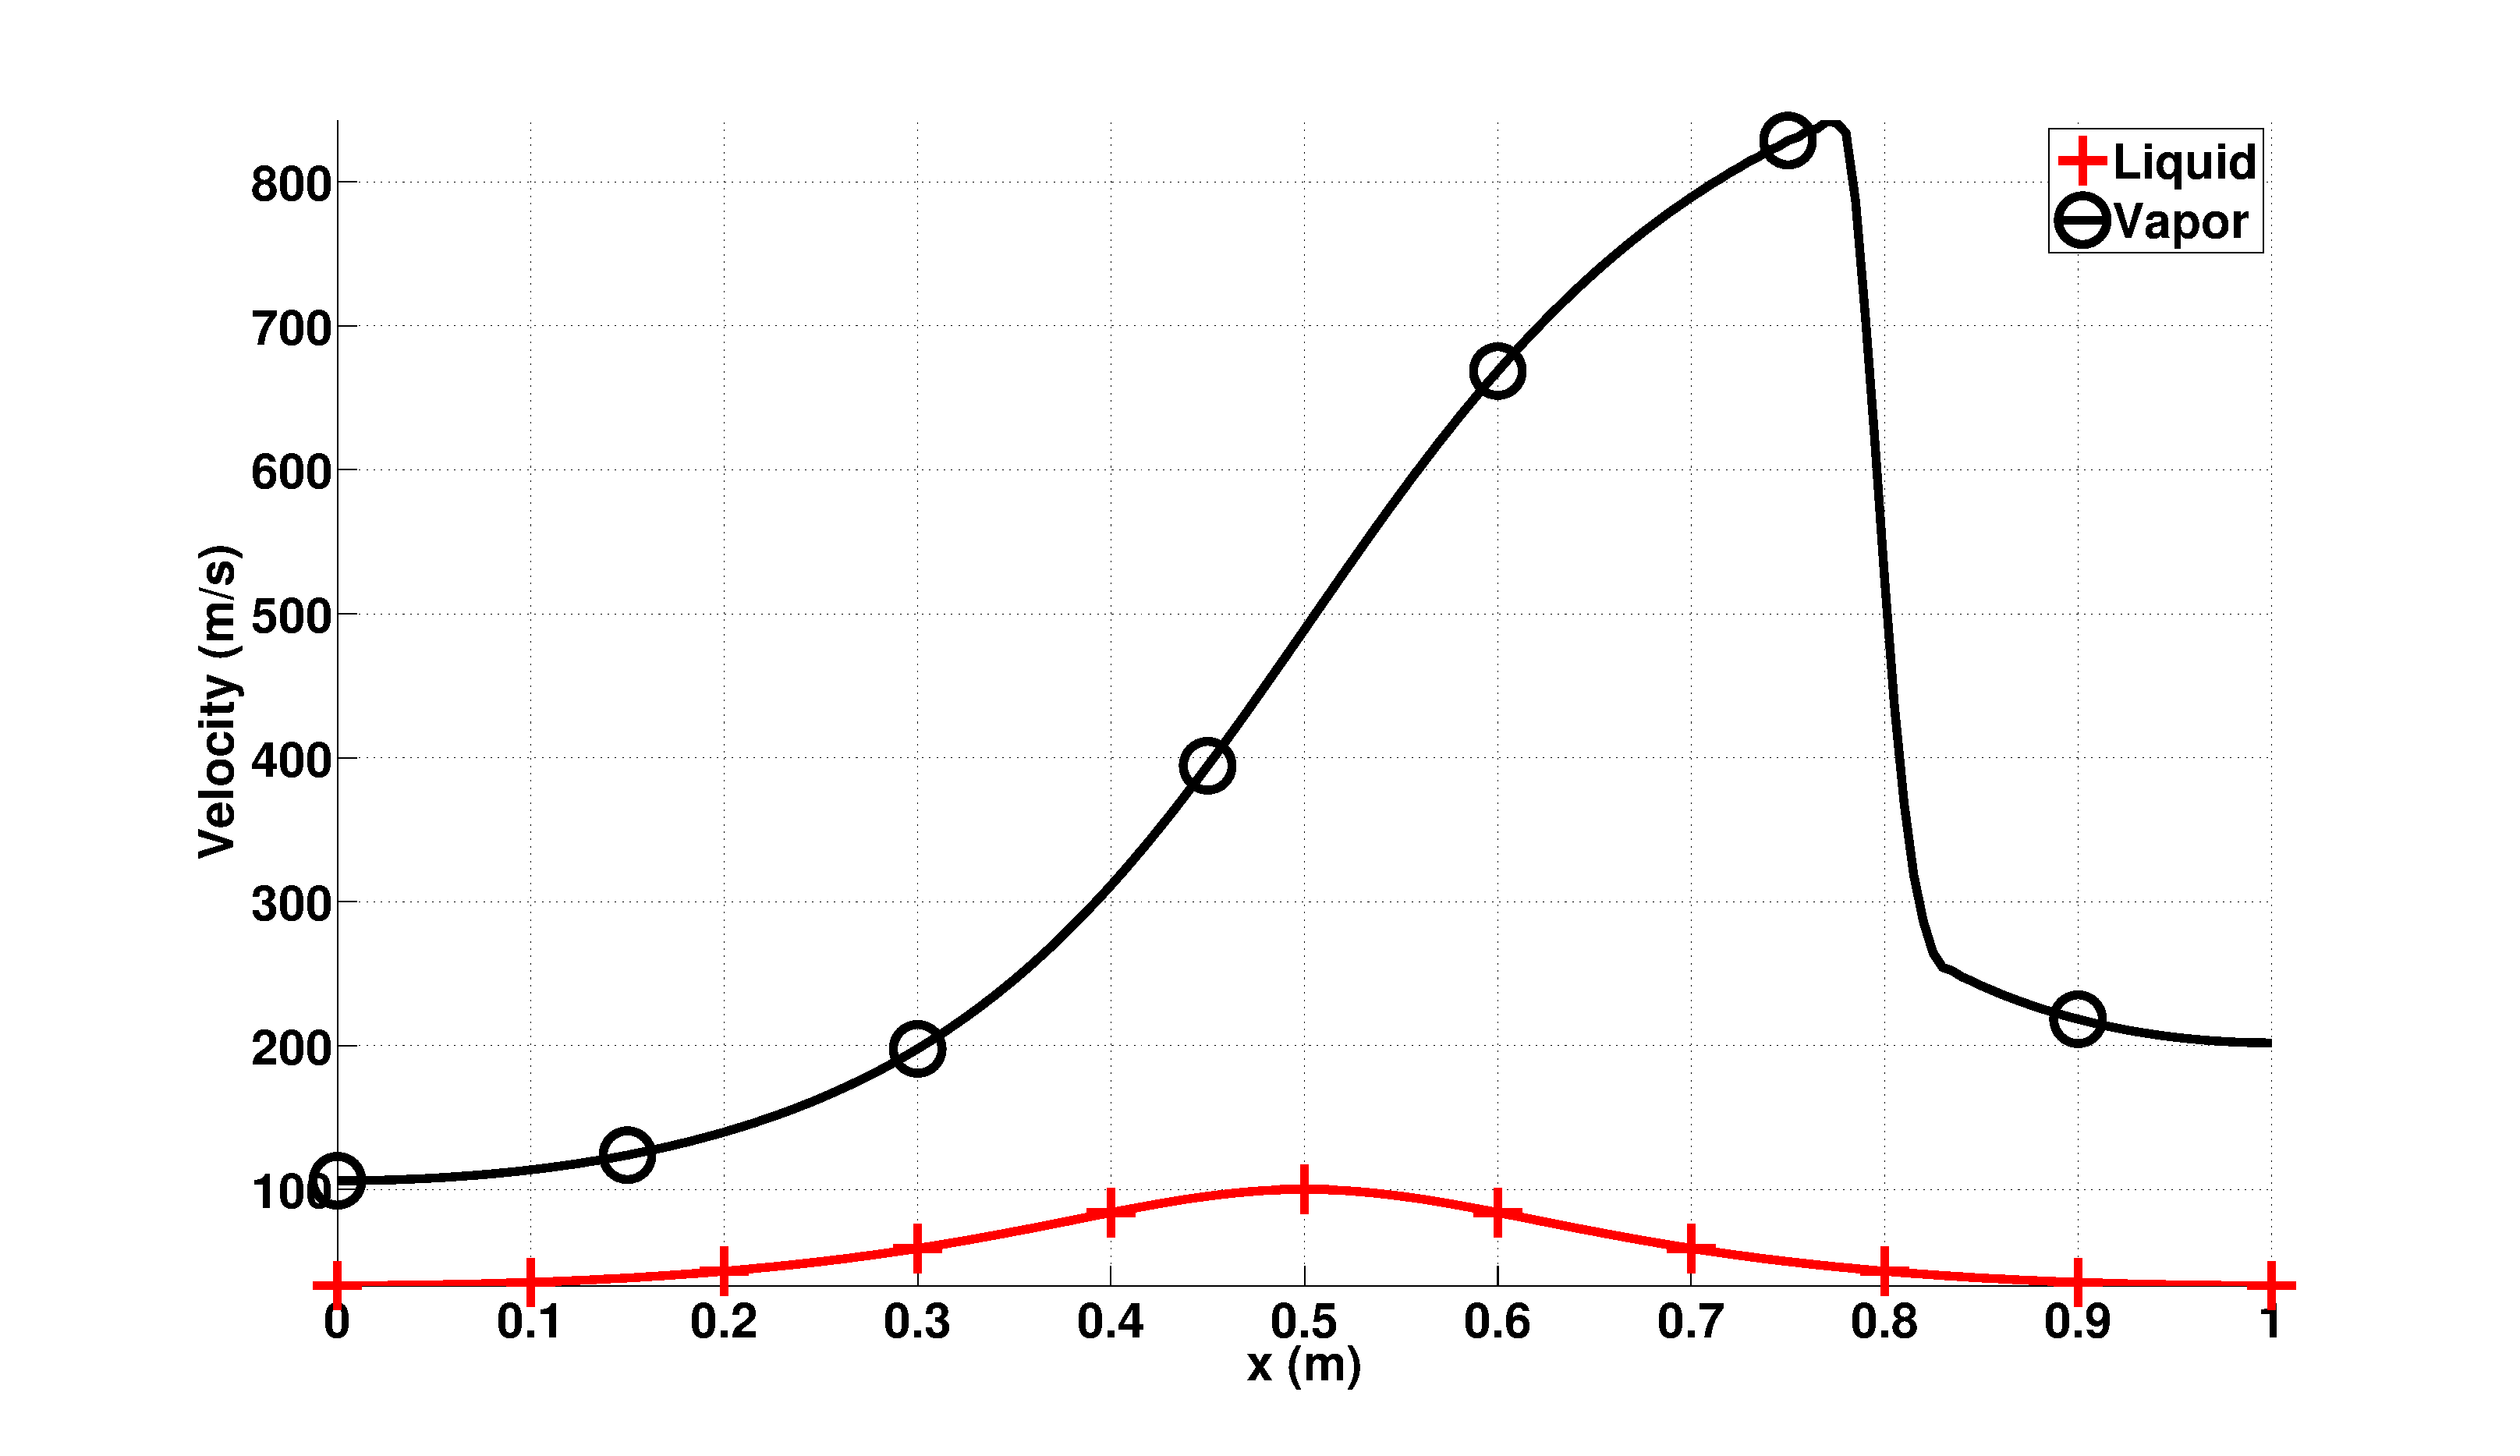
\includegraphics[width=\textwidth]{figures/nozzle-indep-phase_two_phases_velocity.eps}
                \caption{Velocity}
                \label{fig:nozzle-indep-vel}
        \end{subfigure}%

        \begin{subfigure}[b]{0.495\textwidth}
                \centering
                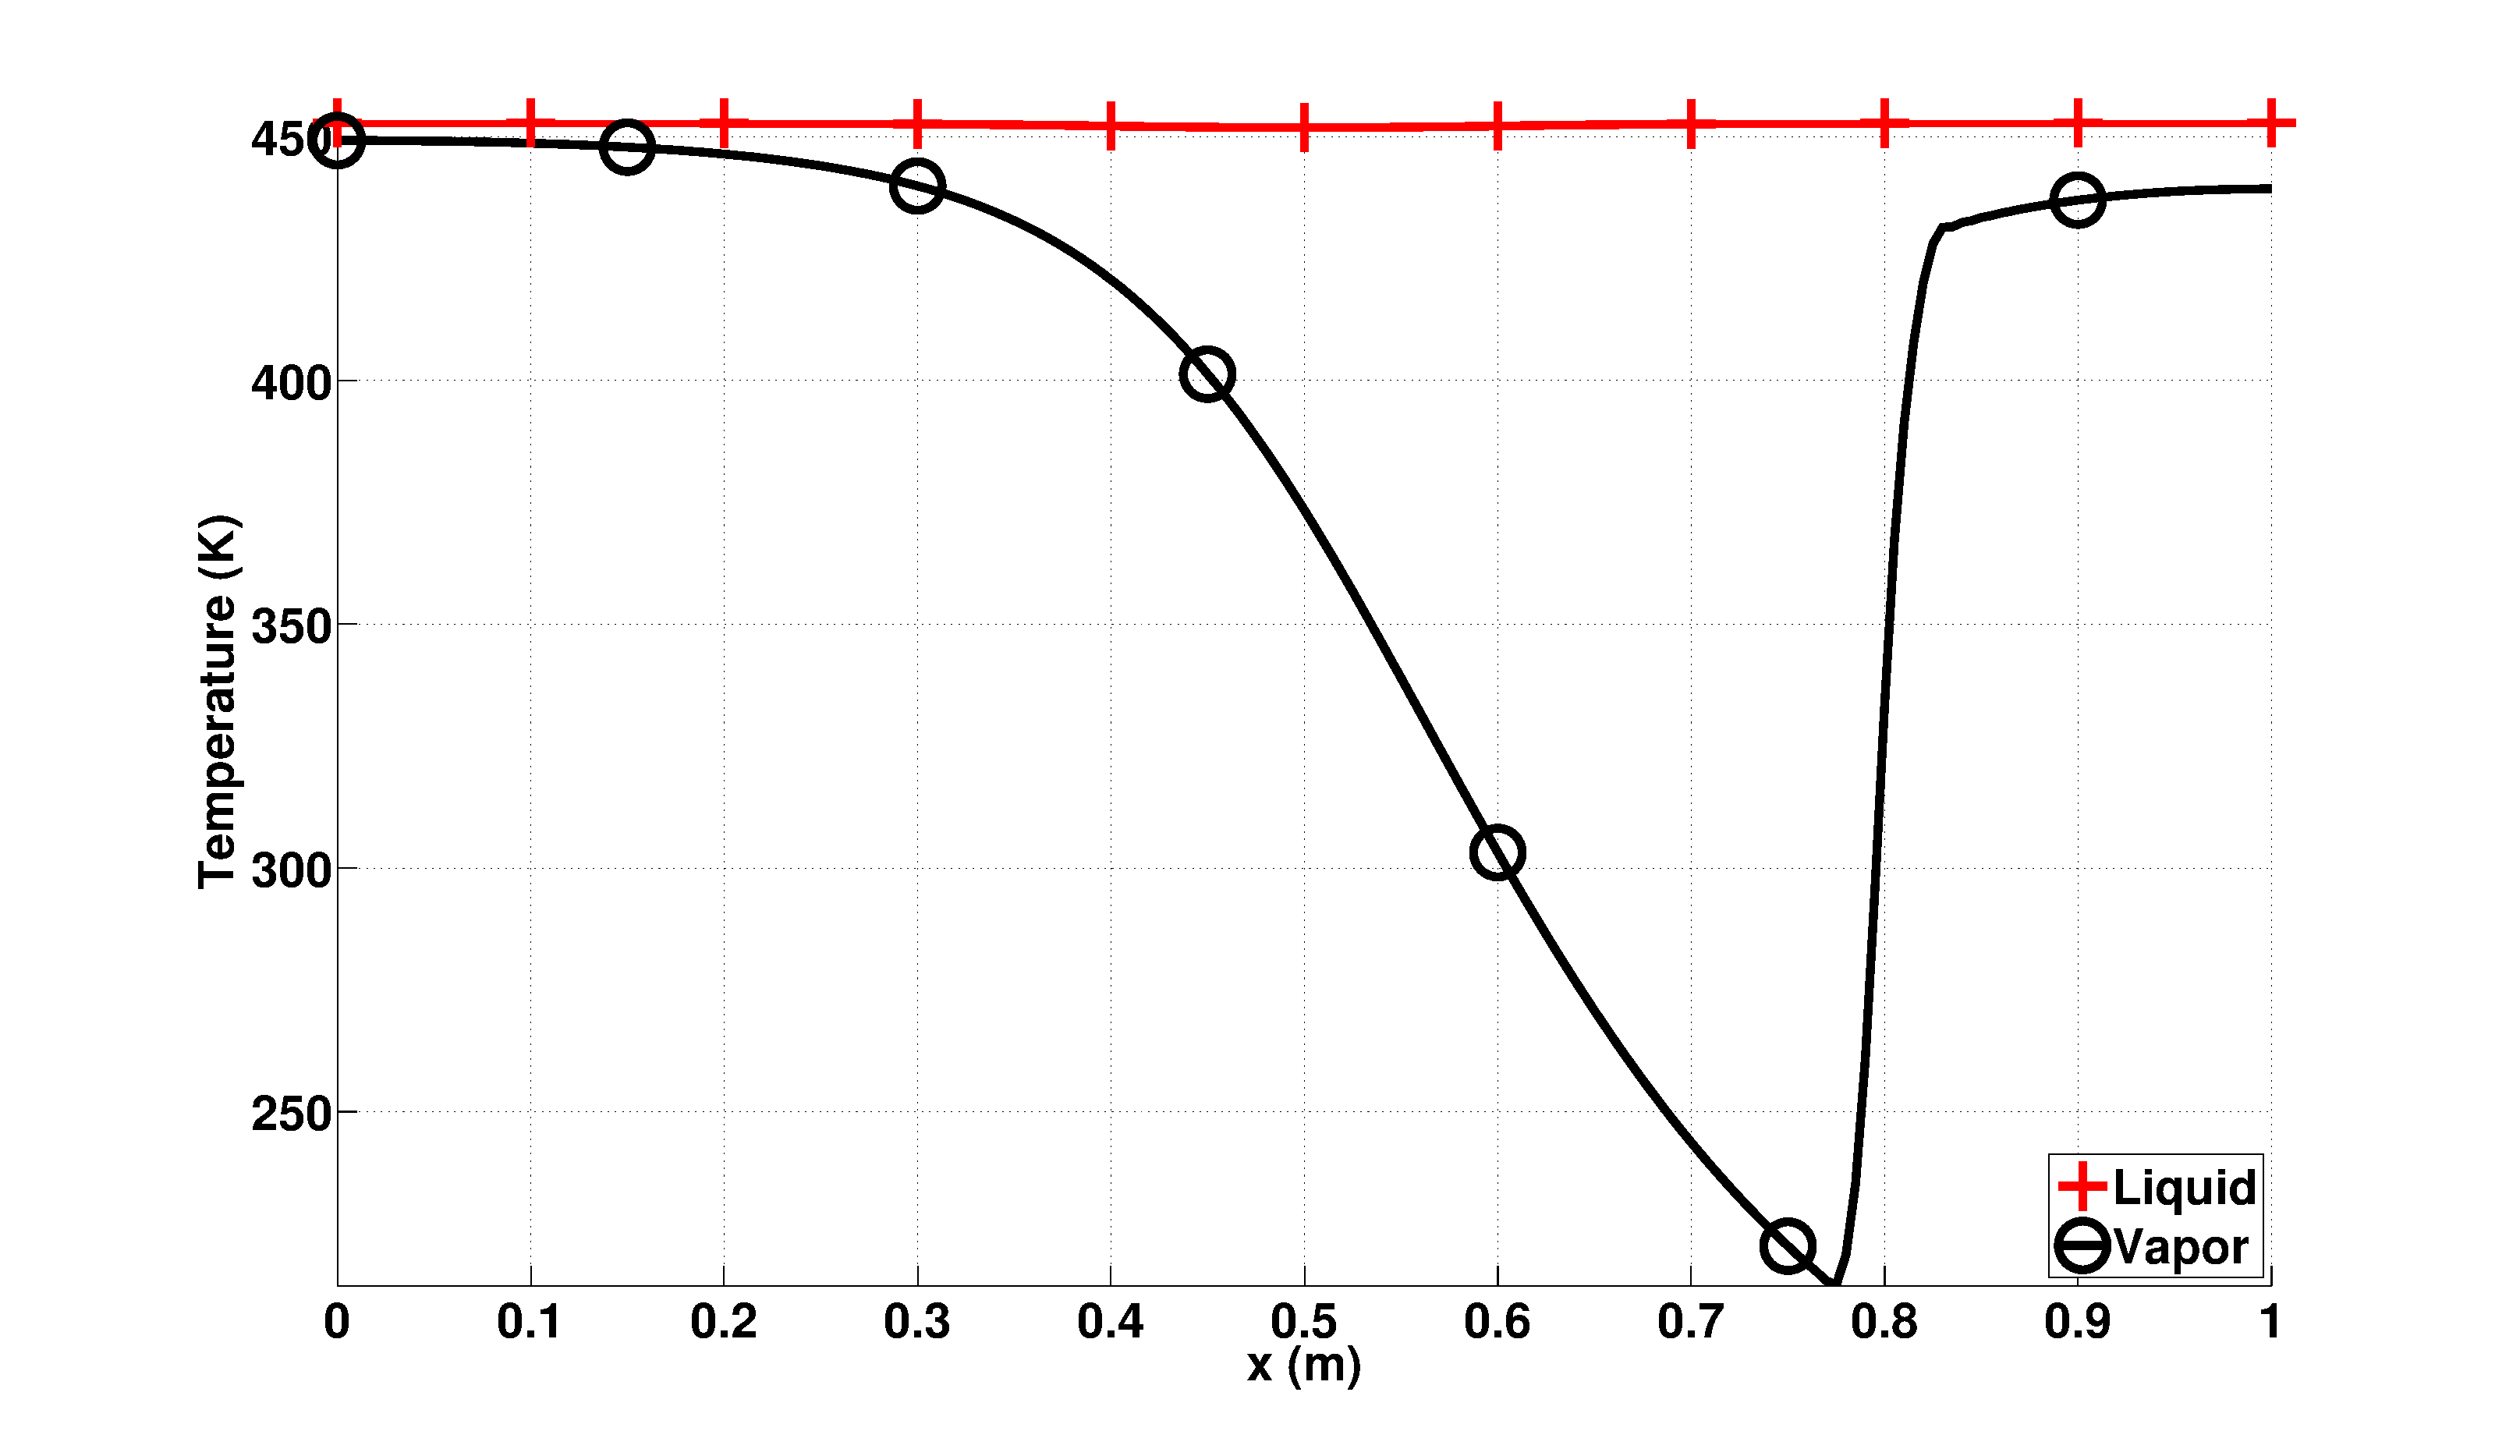
\includegraphics[width=\textwidth]{figures/nozzle-indep-phase_two_phases_temperature.eps}
                \caption{Temperature}
                \label{fig:nozzle-indep-density}
        \end{subfigure}
        \begin{subfigure}[b]{0.495\textwidth}
                \centering
                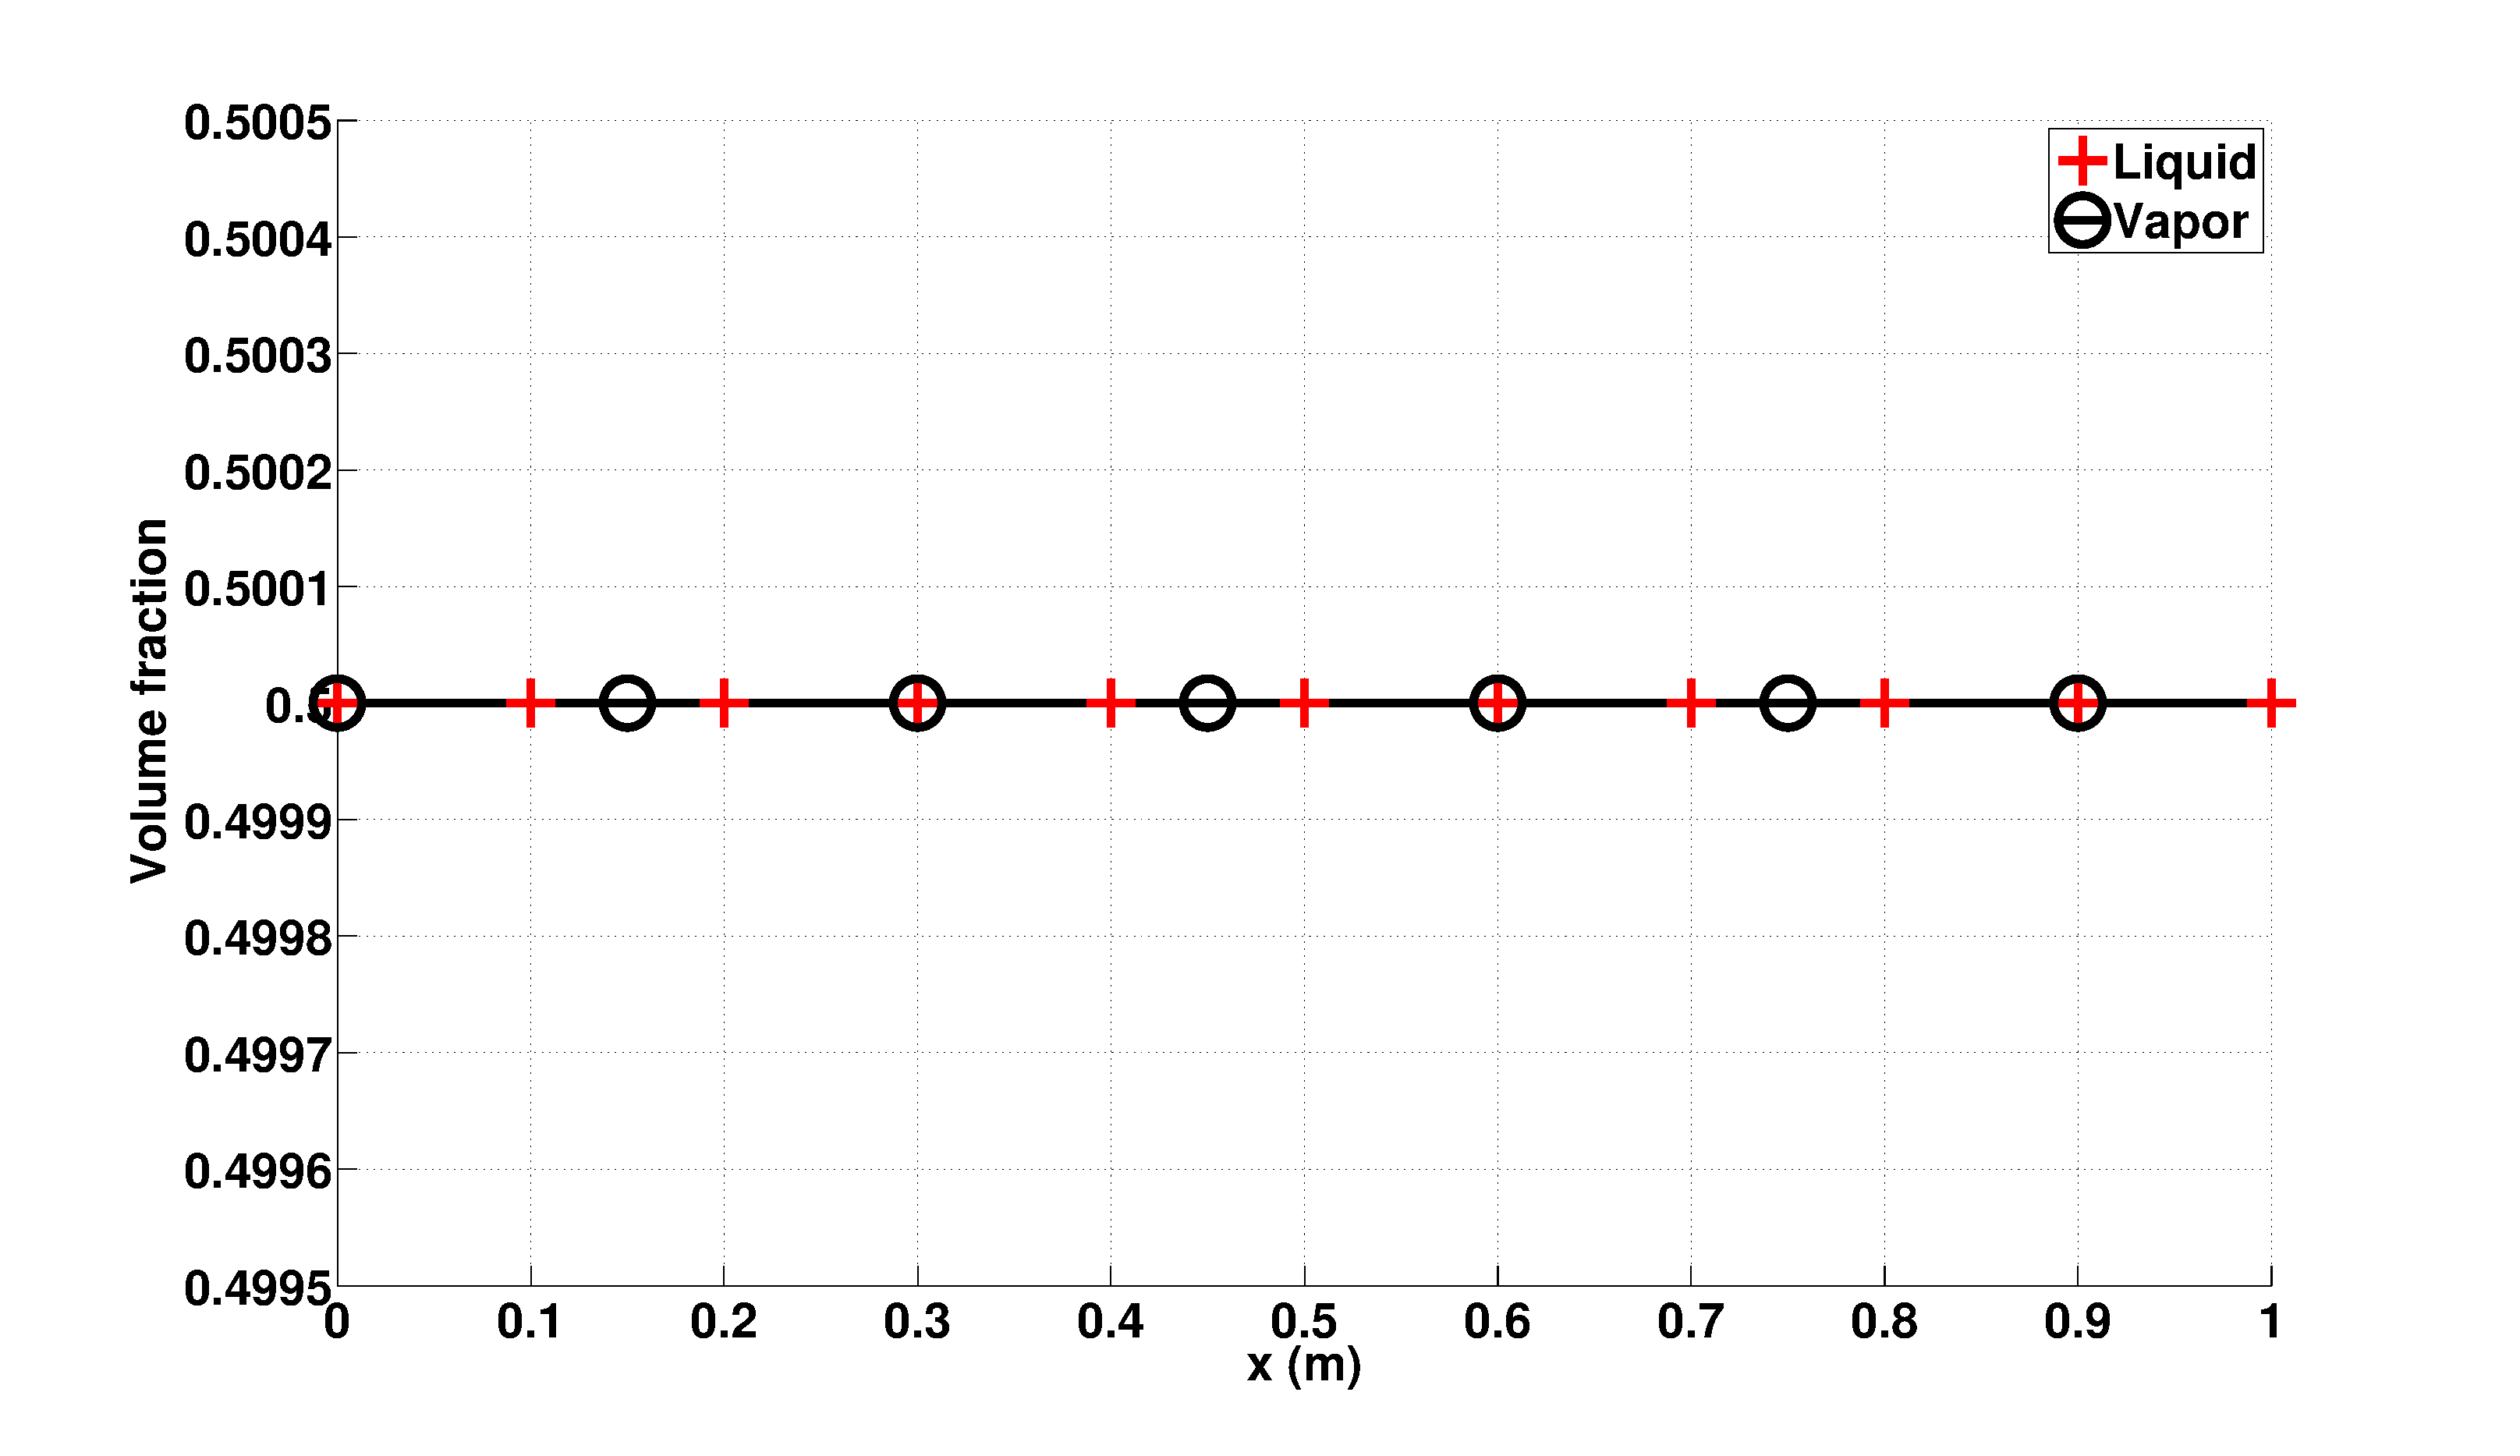
\includegraphics[width=\textwidth]{figures/nozzle-indep-phase_two_phases_volume_fraction.eps}
                \caption{Volume fraction}
                \label{fig:nozzle-indep-vf}
        \end{subfigure}
        \caption{Numerical steady-state solution of two independent flows in a $1$-D converging-diverging nozzle at steady state.}\label{fig:nozzle-indep-variables}
\end{figure}
%
As seen in \fig{fig:nozzle-indep-variables}, the numerical solutions perfectly match the exact solution at steady-state. The steady-state solution of the vapor phase exhibits a shock around $x=0.8 \ m$ and matches the exact solution. Once again, the volume fraction remains constant as expected since the relaxation terms are set to zero. 
%
\begin{figure}[H]
        \centering
        \begin{subfigure}[b]{0.495\textwidth}
                \centering
                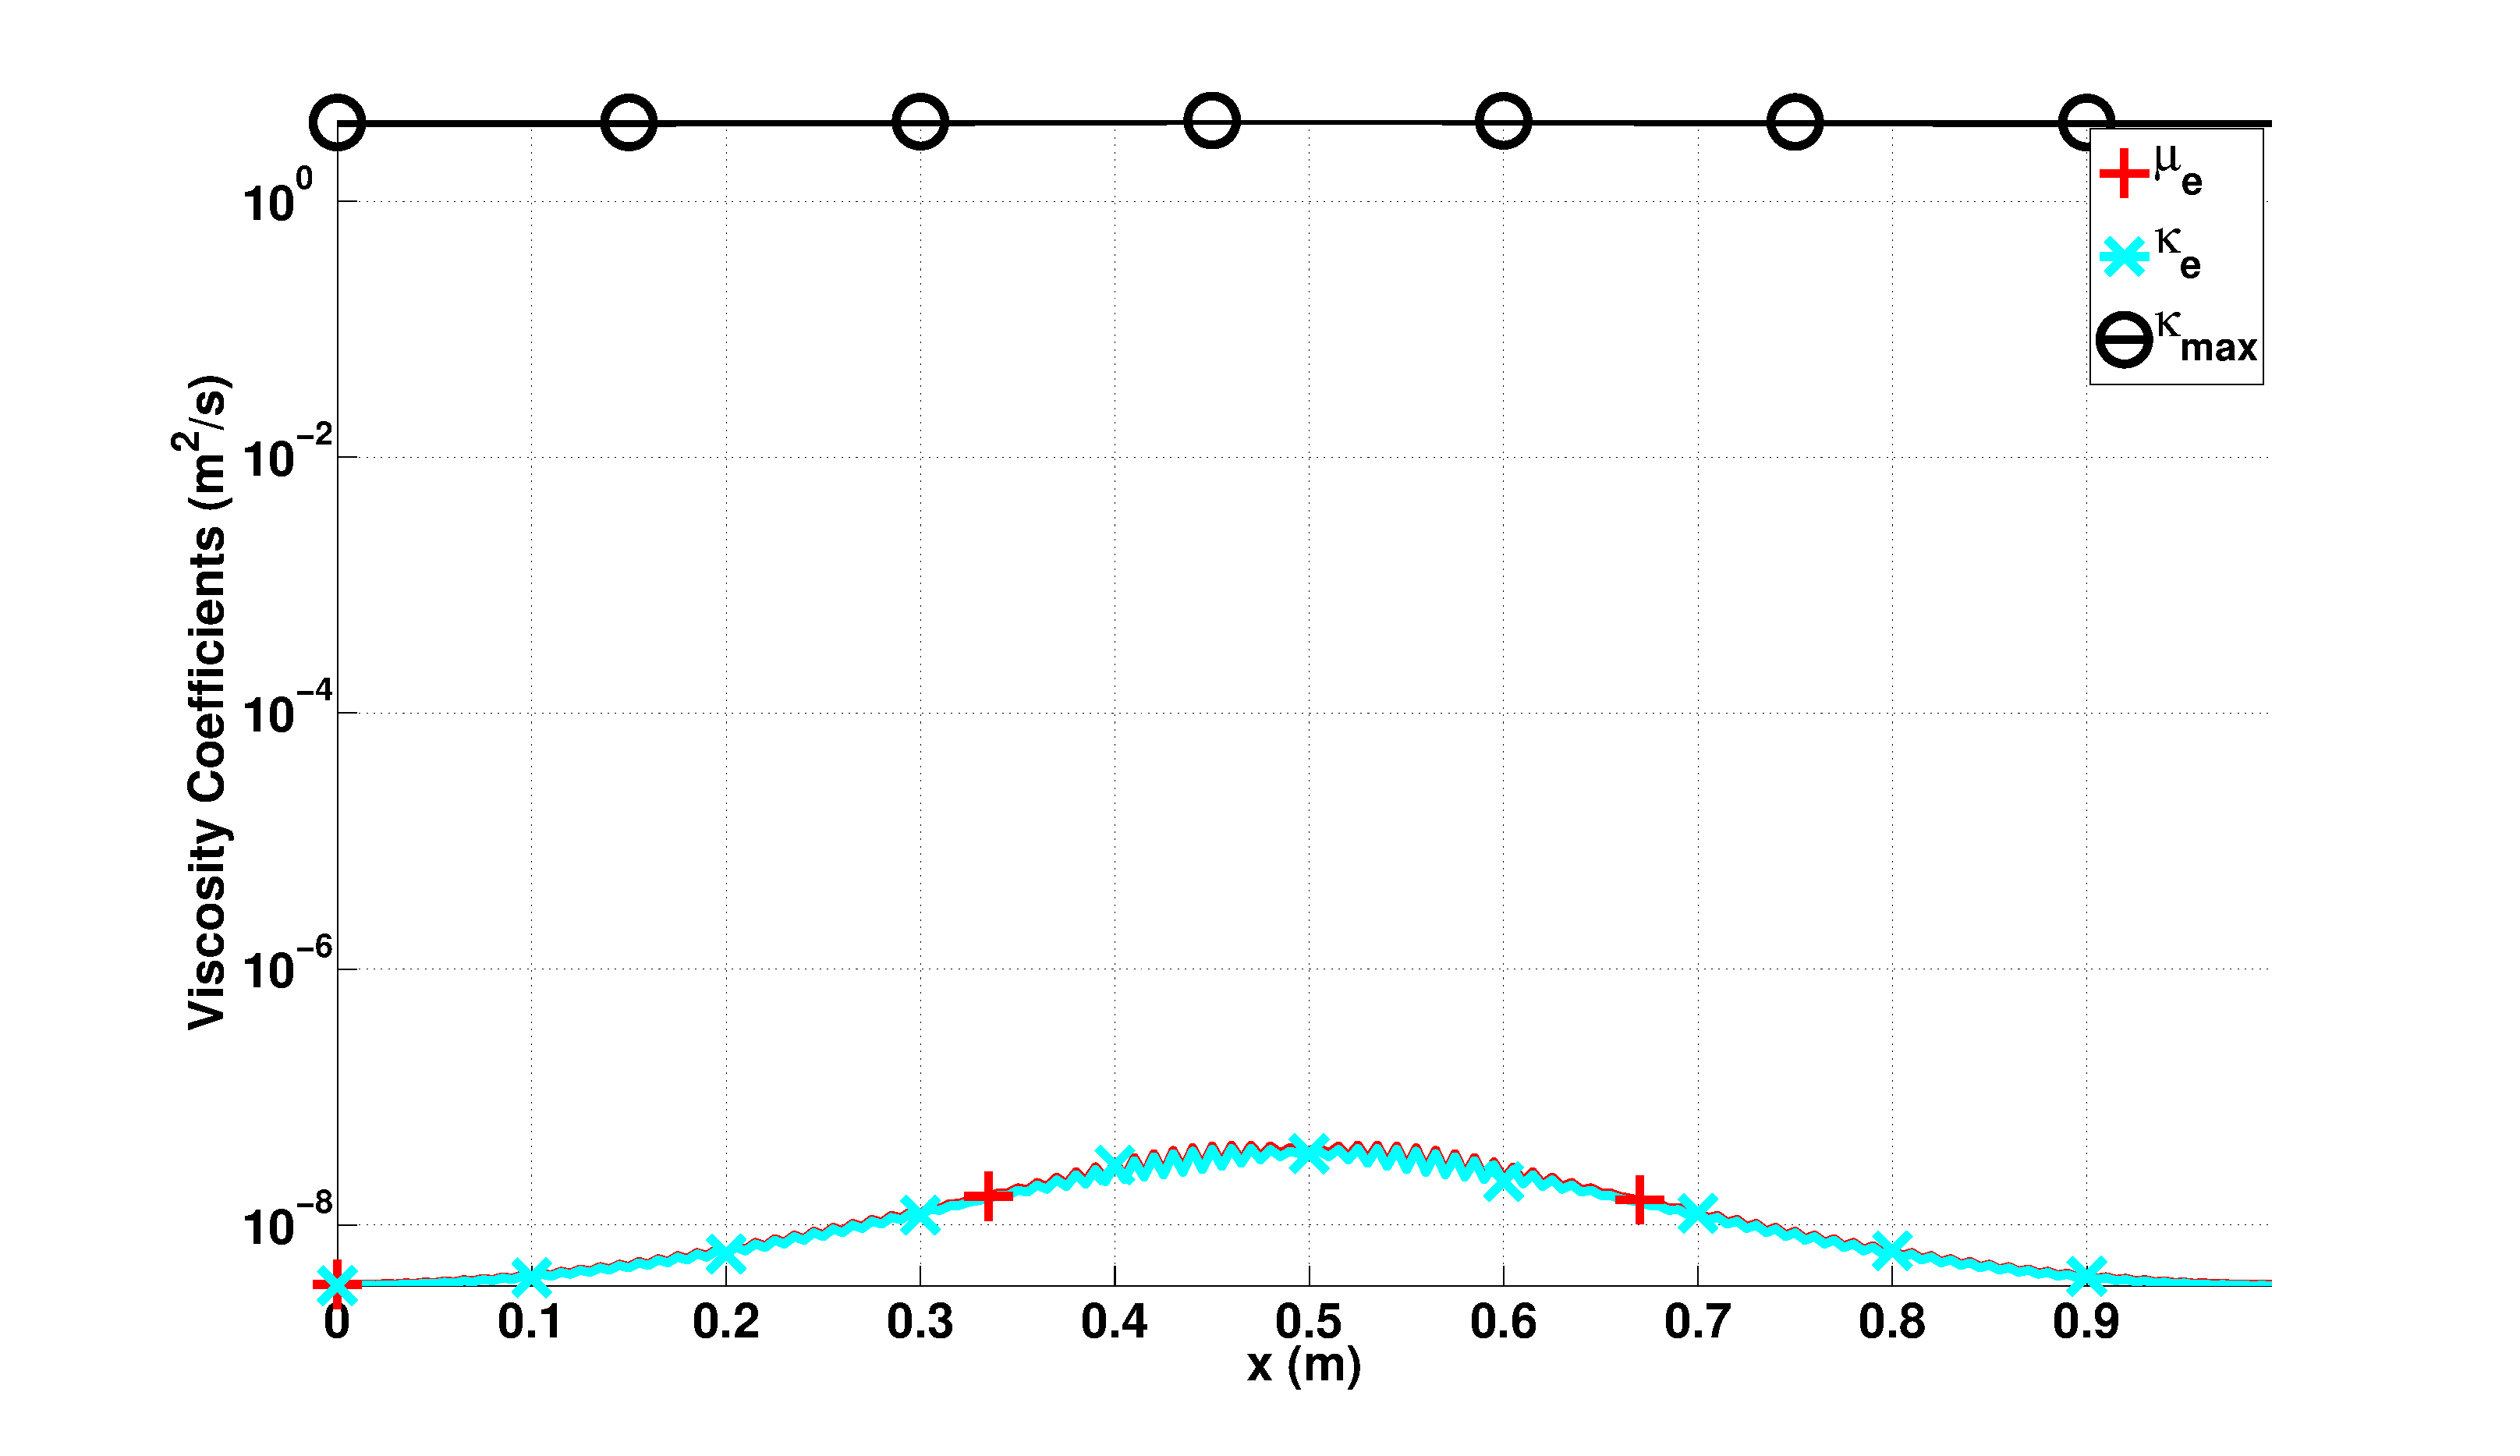
\includegraphics[width=\textwidth]{figures/nozzle-indep-phase_liquid_viscosity_kappa_mu.eps}
                \caption{Viscosity coefficients for phase 1.}
                \label{fig:nozzle-indep-visc-coeff-phase-1}
        \end{subfigure}%
        \begin{subfigure}[b]{0.495\textwidth}
                \centering
                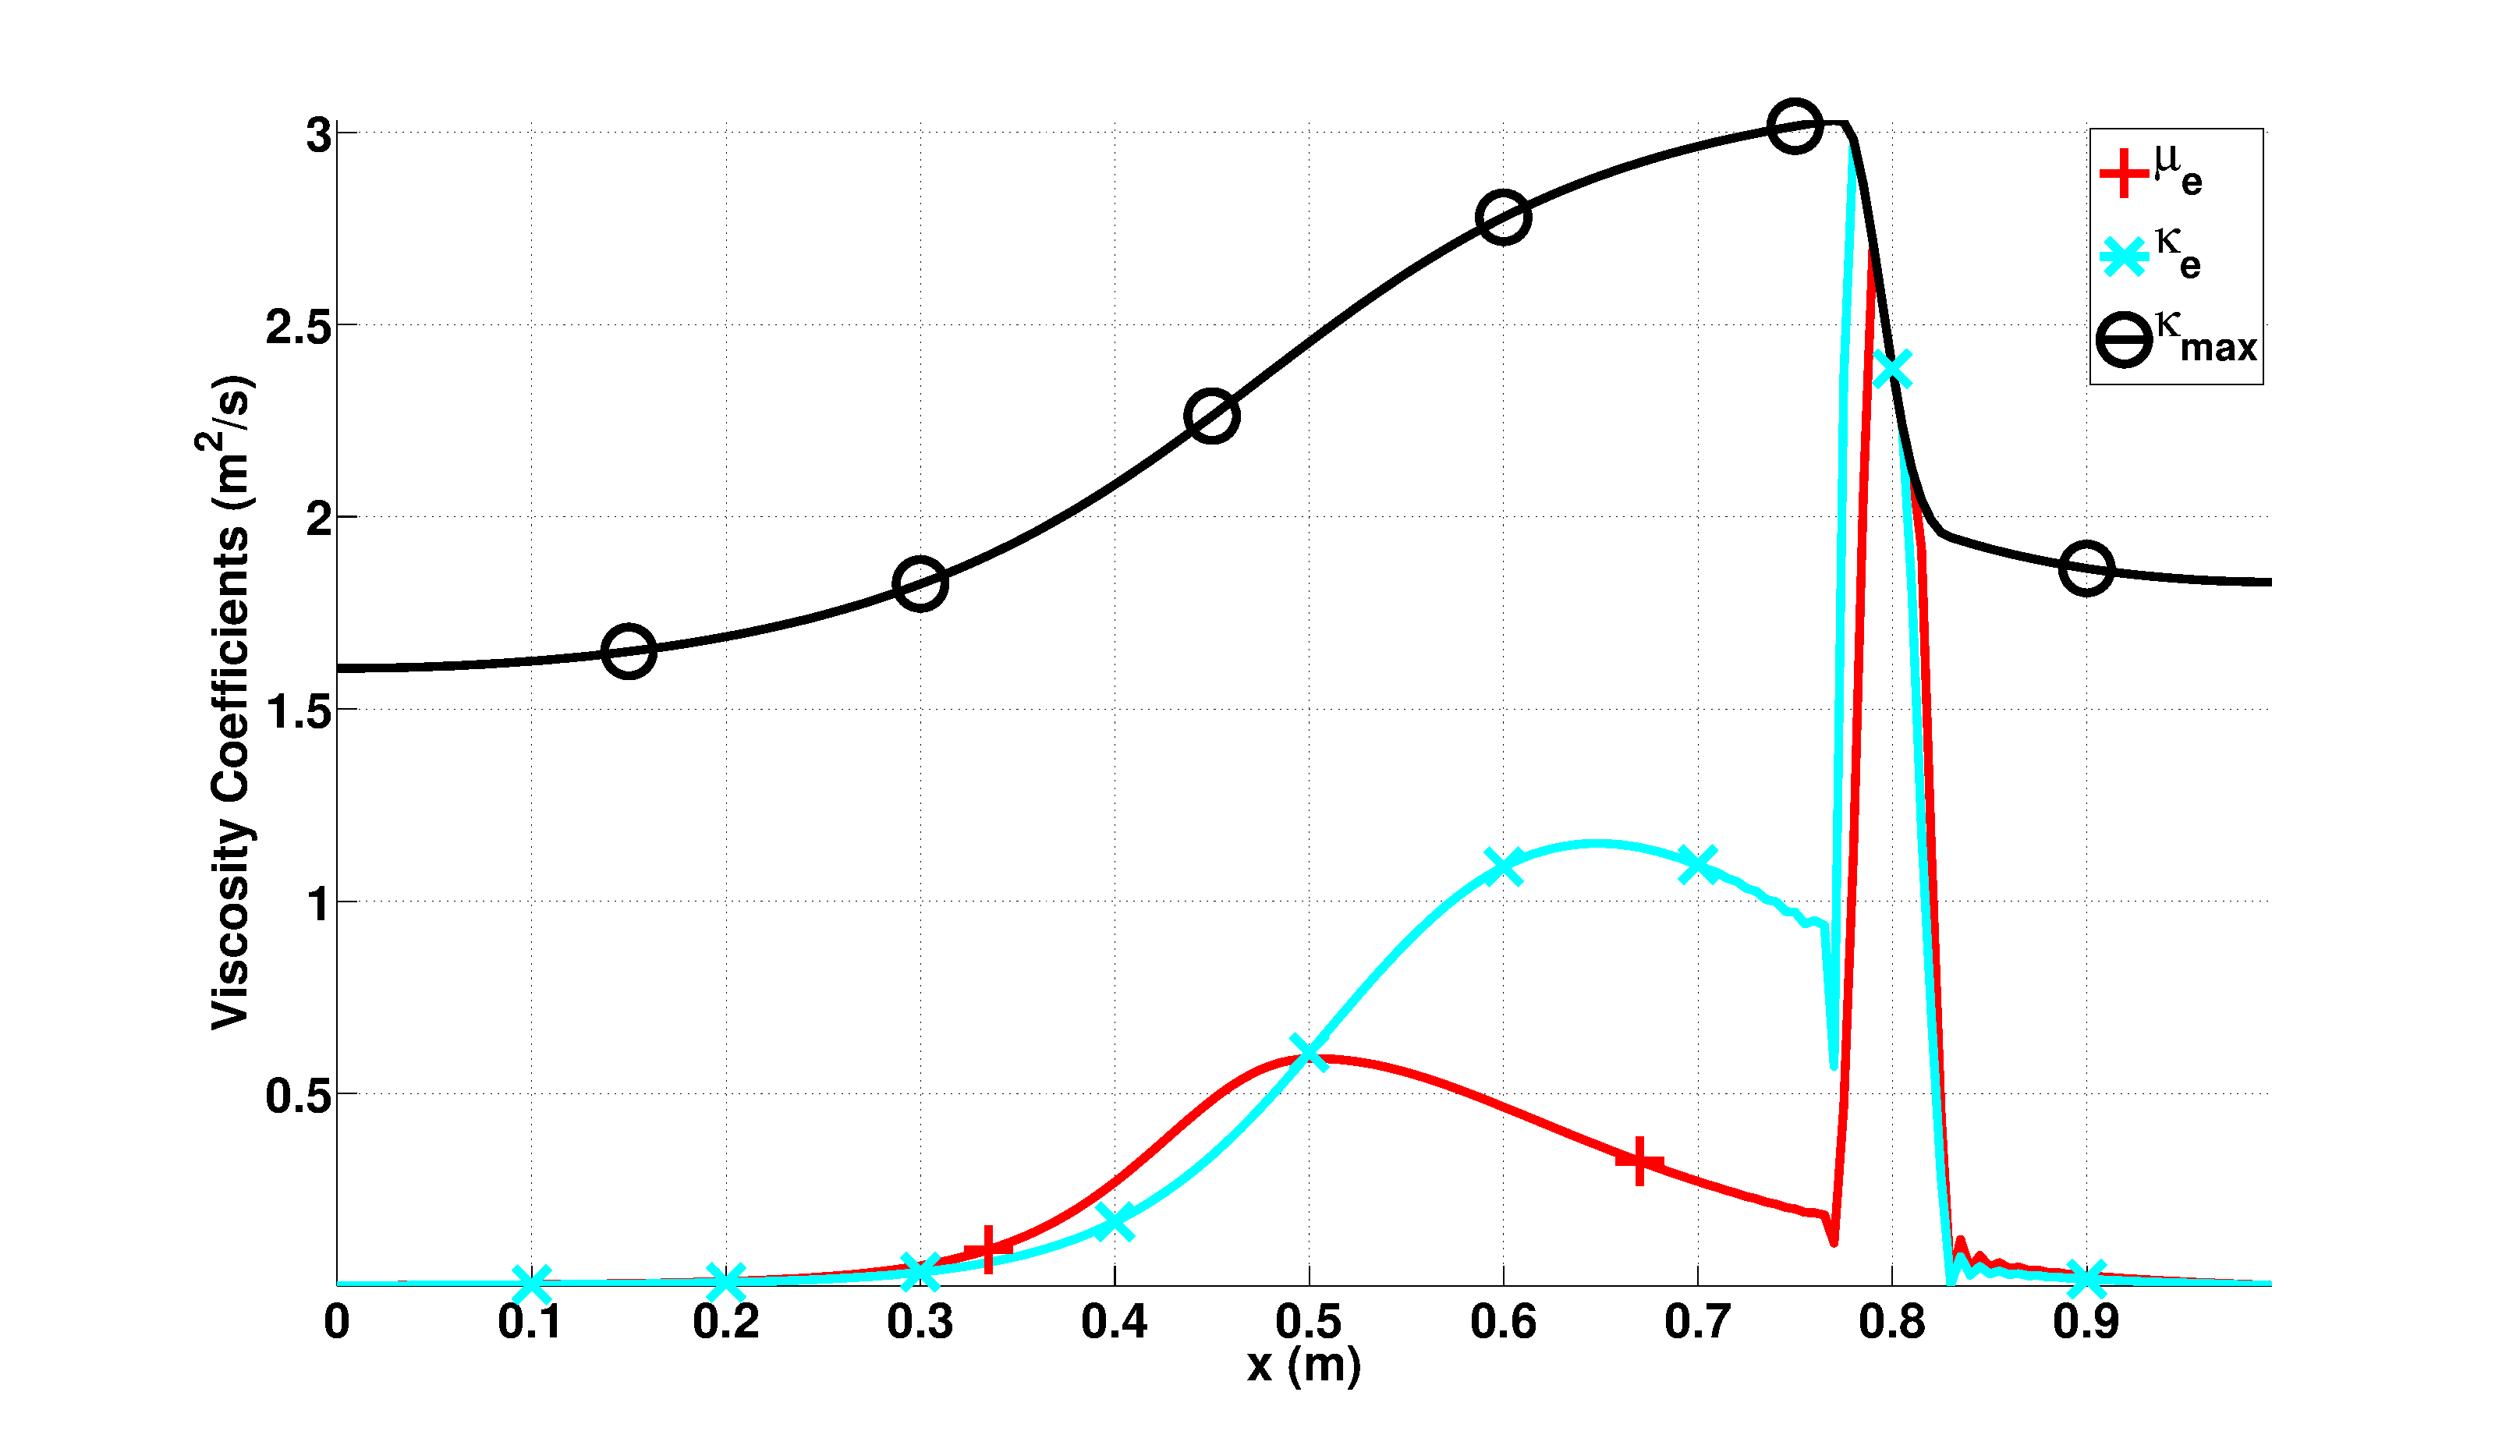
\includegraphics[width=\textwidth]{figures/nozzle-indep-phase_vapor_viscosity_kappa_mu.eps}
                \caption{Viscosity coefficients for phase 2}
                \label{fig:nozzle-indep-visc-coeff-phase-2}
        \end{subfigure}
        
        \begin{subfigure}[b]{0.495\textwidth}
                \centering
                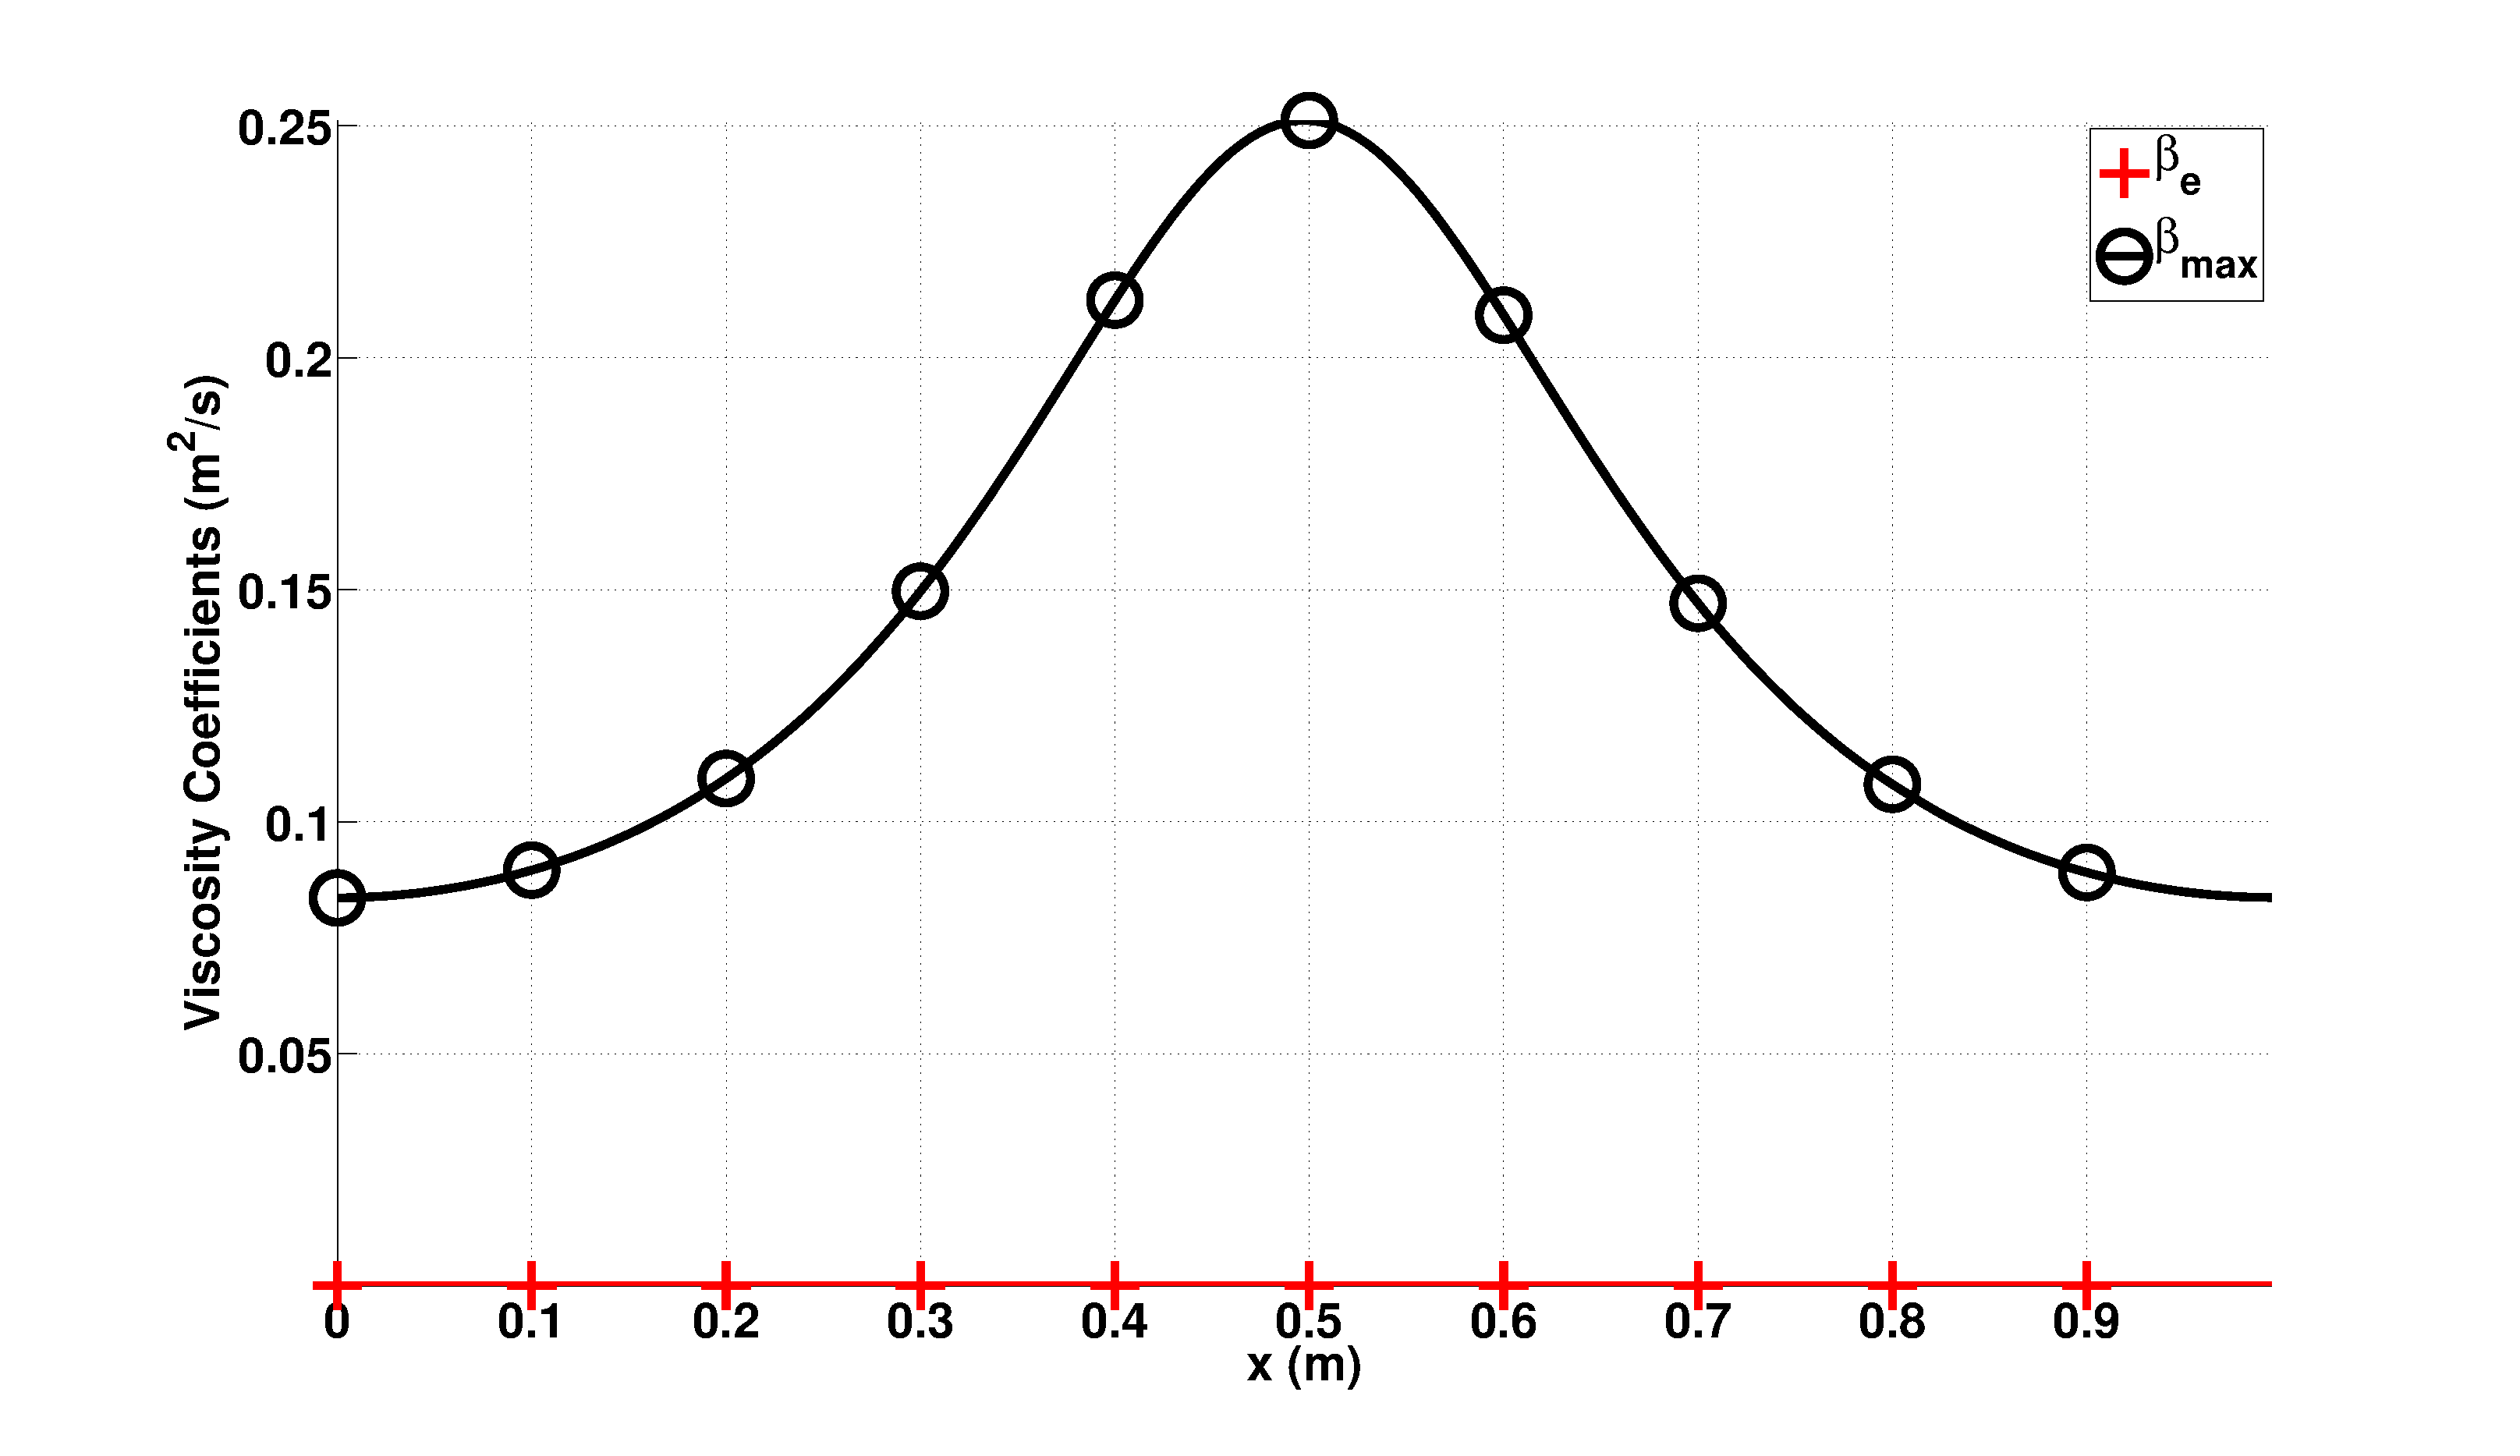
\includegraphics[width=\textwidth]{figures/nozzle-indep-phase_liquid_beta.eps}
                \caption{Viscosity coefficients for the volume fraction equation of phase 1.}
                \label{fig:nozzle-indep-beta}
        \end{subfigure}        
        \caption{Viscosity coefficients profiles of two independent flows in a $1$-D converging-diverging nozzle at steady state.}\label{fig:nozzle-indep-visc-coeff}
\end{figure}
%
The viscosity coefficients of the liquid phase as shown in \fig{fig:nozzle-indep-visc-coeff-phase-1} on a log-scale plot: note that the entropy viscosity coefficient is very small compared to the first-order one because 
(i) the numerical solution is smooth as shown in \fig{fig:nozzle-indep-visc-coeff-phase-1} and (ii) the flow is in a isentropic low-Mach regime (subsonic flow). 
In \fig{fig:nozzle-indep-visc-coeff-phase-2}, 
the first-order and entropy viscosity coefficients are plotted at steady state (on a log scale): the entropy viscosity 
coefficient is peaked in the shock region around $x=0.8 \ m$ where it saturates to the first-order viscosity 
coefficient denoted by the subscript $max$. Elsewhere, the entropy  viscosity coefficient is small. The viscosity coefficient profile of $\beta_e$ is given in \fig{fig:nozzle-indep-beta} and is zero as the volume fraction profile is constant. A convergence study was performed in \cite{Marco_paper_low_mach} for this particular test and showed the expected convergence rate for the L$_1$ and L$_2$ norms.
%
%%%%%%%%%%%%%%%%%%%%%%%%%%%%%%%%%%%%%
\subsubsection{Fluids in a 1-D converging-diverging nozzle with infinite relaxation terms}\label{sec:nozzle-infinite-rel-coeff}
%%%%%%%%%%%%%%%%%%%%%%%%%%%%%%%%%%%%%
%
We still consider a two-phase flow in a $1$-D converging-diverging nozzle with the same initial conditions as in \sct{sec:nozzle-two-indep-fluids} but with the relaxation terms turned on:  
the pressure and velocity relaxation coefficients are computed from \eqt{eq:Aint-def} and \eqt{E-R:86} with $A_{int,max} =  
10^4$ $m^{-1}$: $\mu_P \sim 4$ and $\lambda_u \sim 5 \times 10^5$ $s^{-1}$. A stagnation pressure boundary condition is set at the inlet with $P_0 = 1 \ MPa$ and $T_0 = 453 \ K$ for both phases. At the outlet, a static pressure boundary condition is used with $P_s = 0.5 \ MPa$ for both phases also. The numerical results are given in \fig{fig:nozzle-aint-1e4-variables} along with the corresponding viscosity coefficients in \fig{fig:nozzle-aint-1e4-visc-coeff}. The initial conditions are computed from the boundary conditions by assuming the two fluids at rest and linearly interpolating the pressure and temperature between the boundary values.
%
\begin{figure}[H]
        \centering
        \begin{subfigure}[b]{0.495\textwidth}
                \centering
                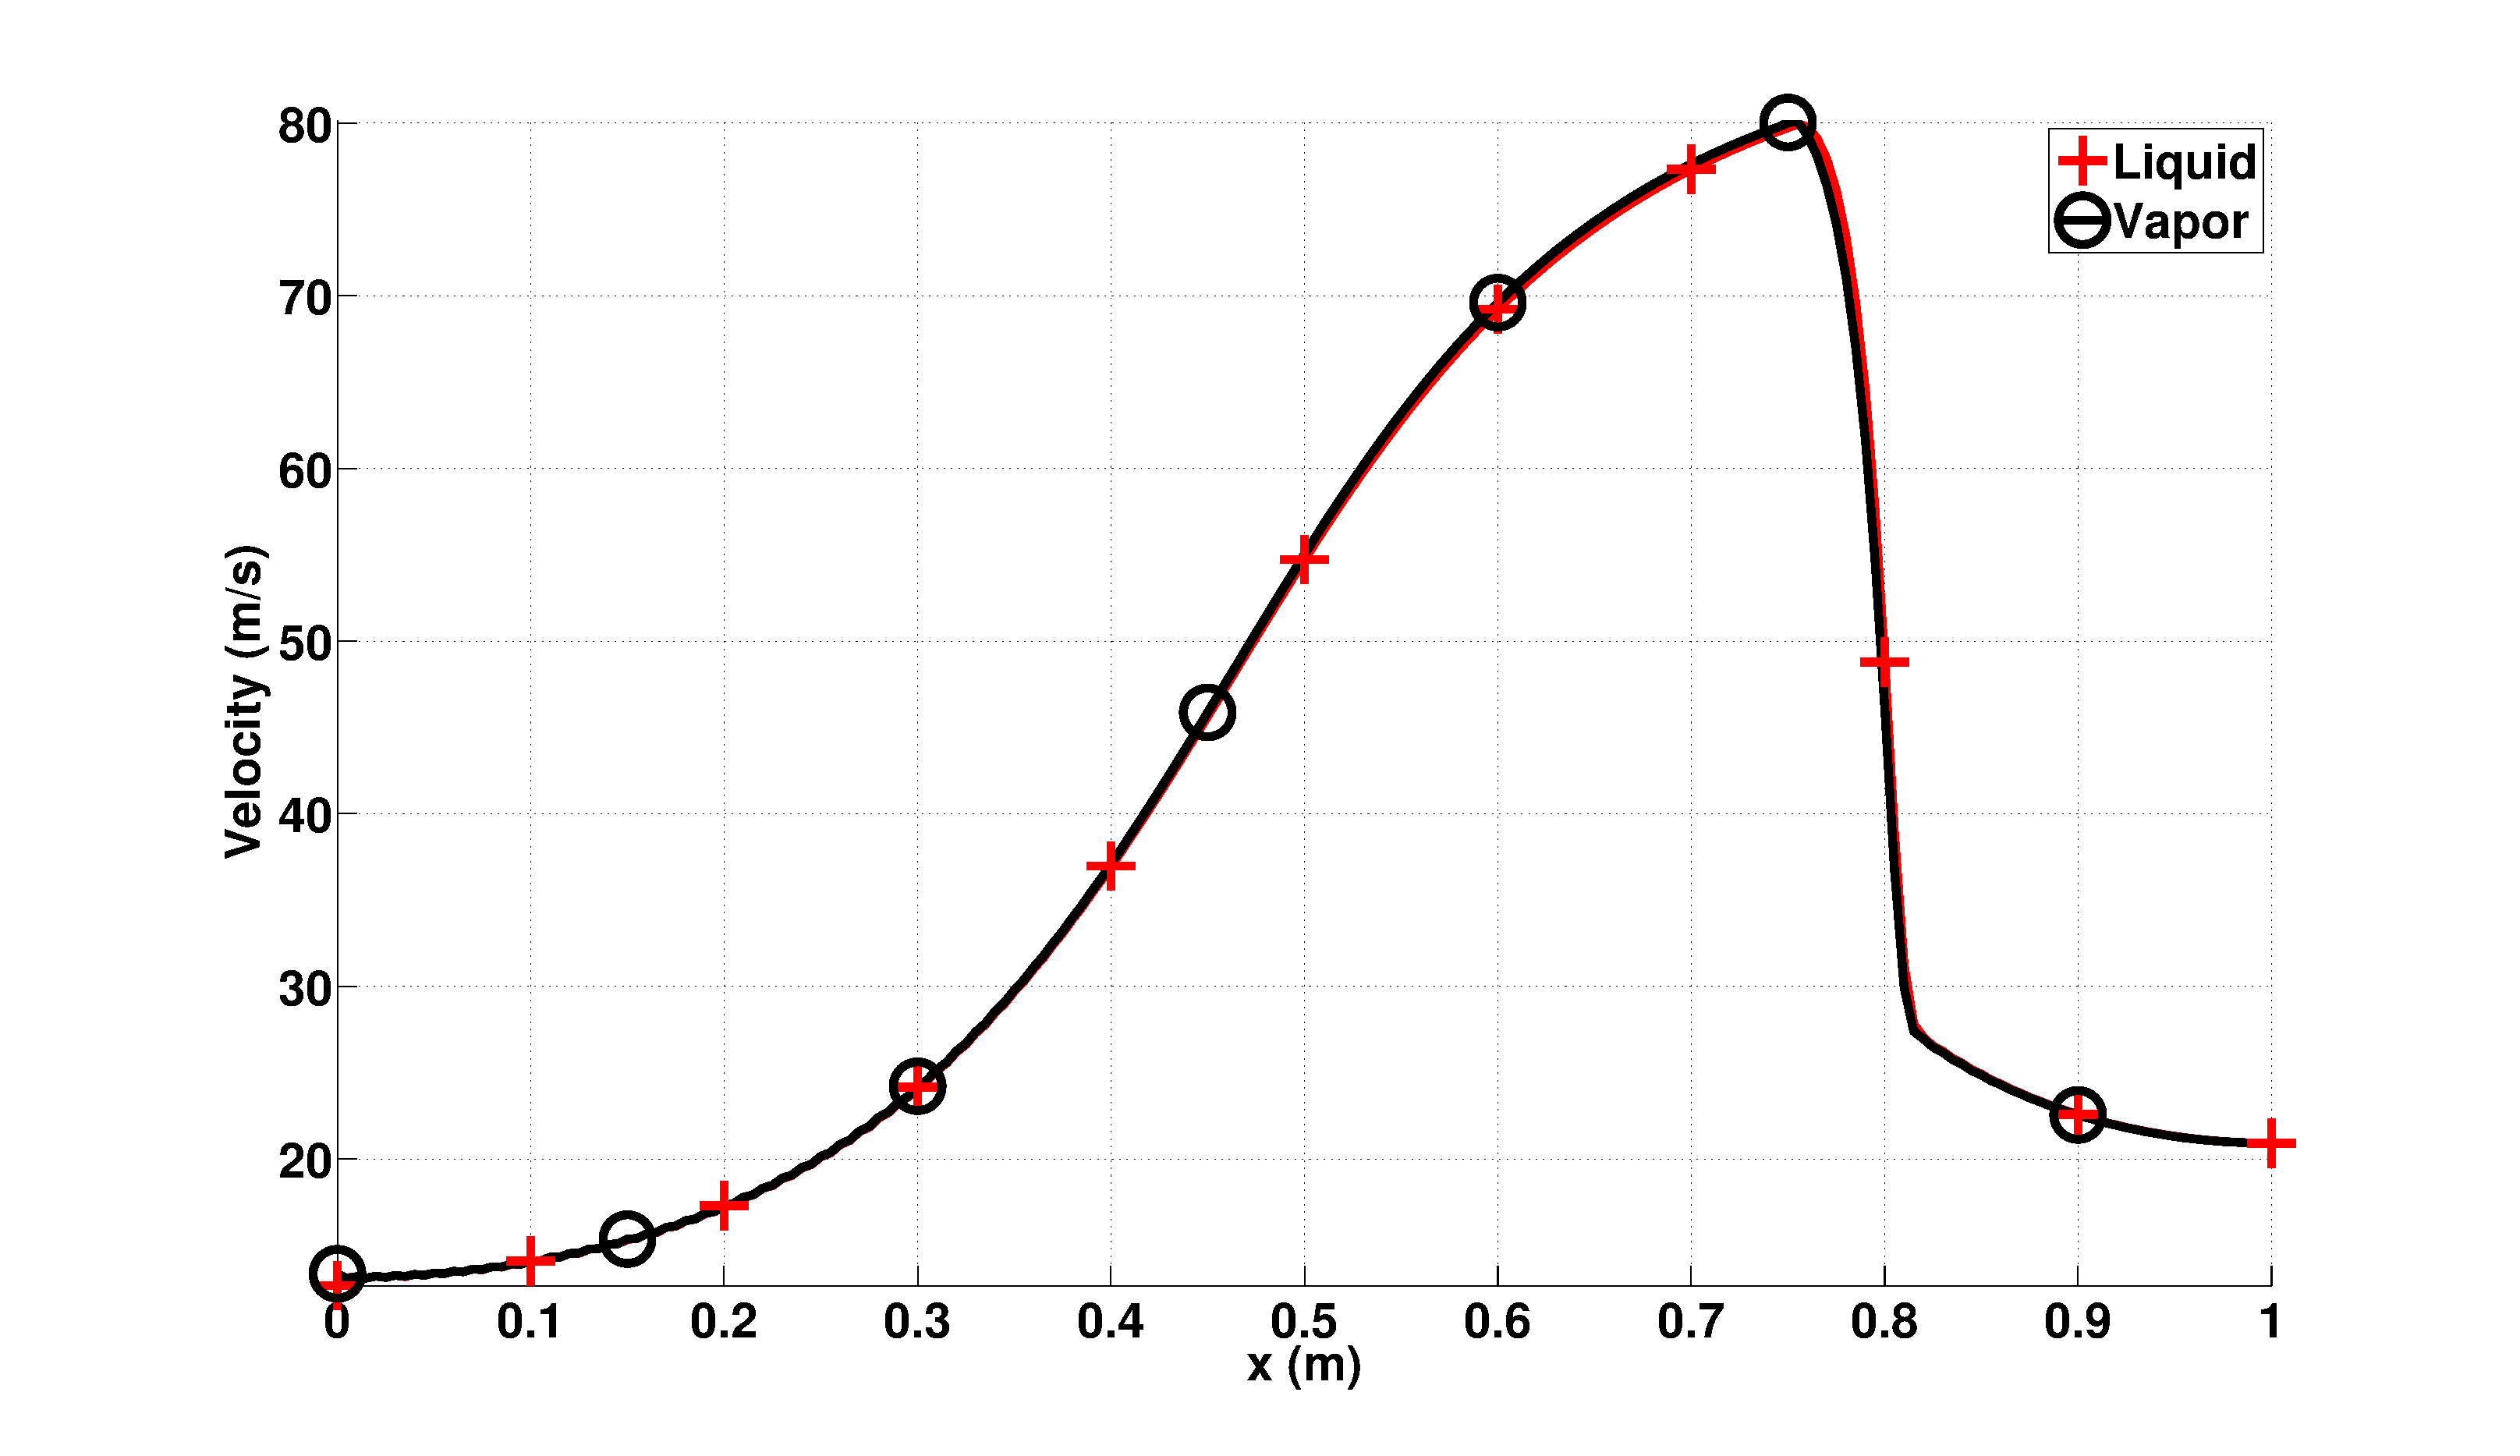
\includegraphics[width=\textwidth]{figures/nozzle-aint-1e4_two_phases_velocity.eps}
                \caption{Velocity}
                \label{fig:nozzle-aint-1e4-vel}
        \end{subfigure}%
        \begin{subfigure}[b]{0.495\textwidth}
                \centering
                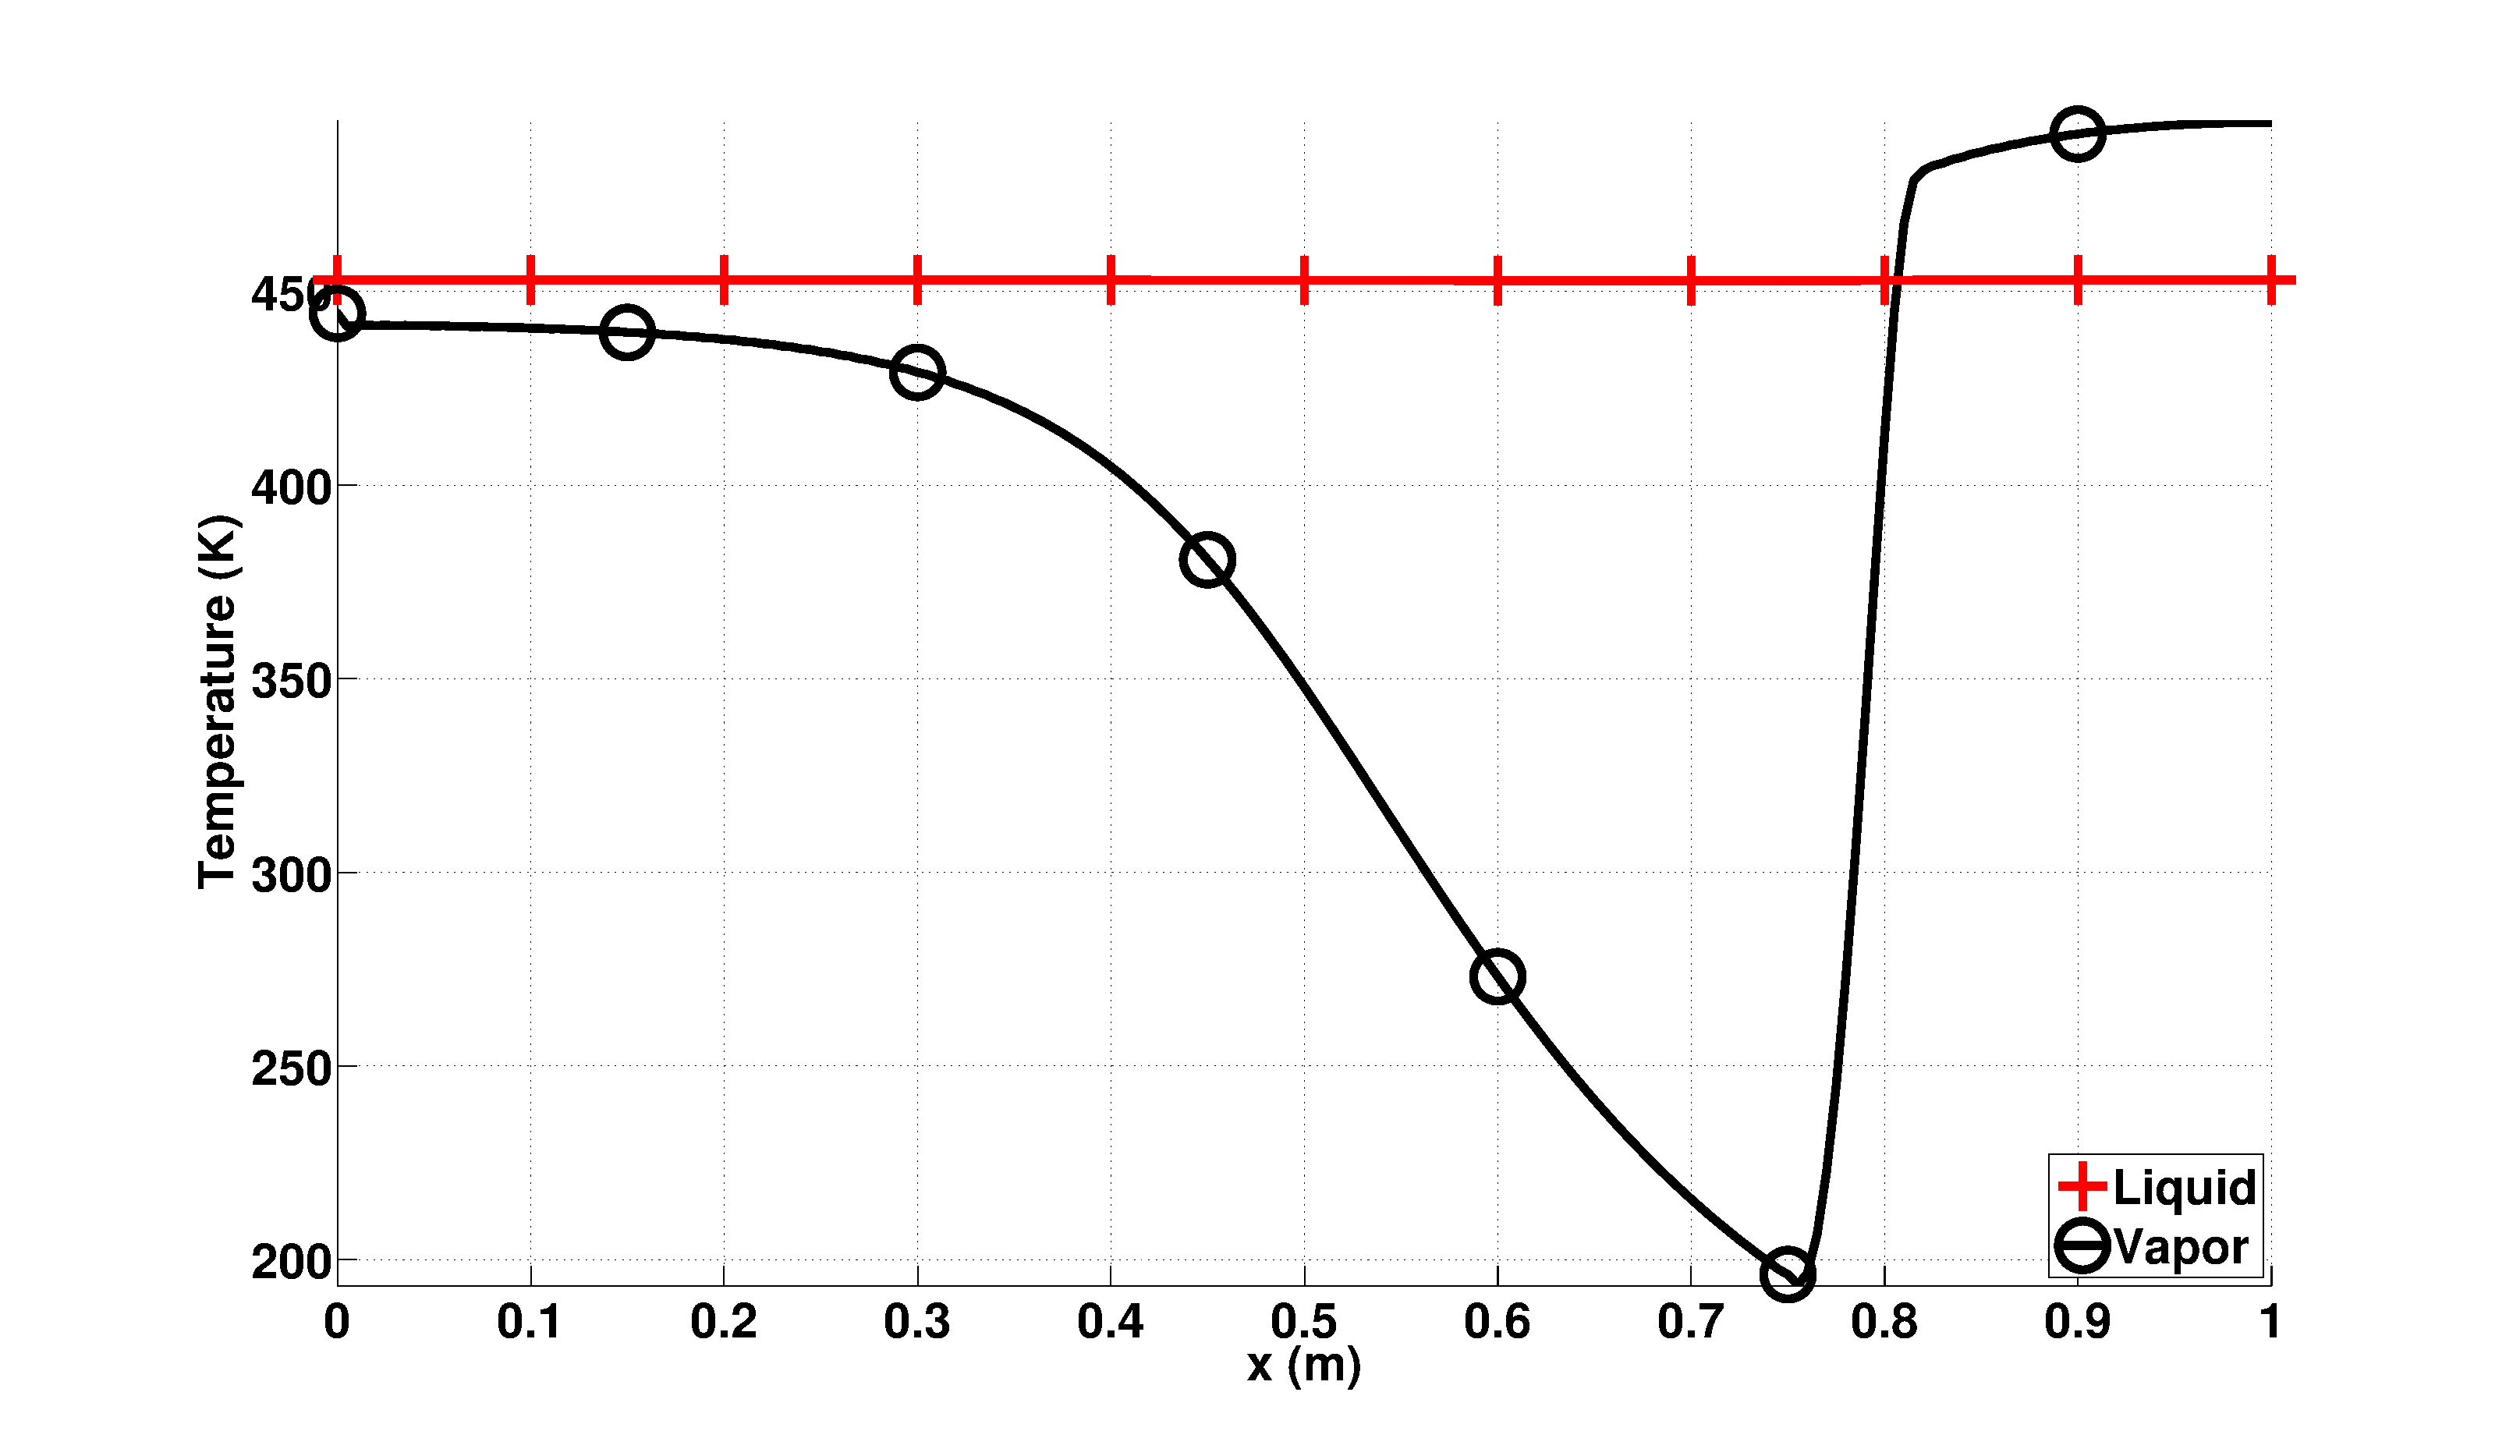
\includegraphics[width=\textwidth]{figures/nozzle-aint-1e4_two_phases_temperature.eps}
                \caption{Temperature}
                \label{fig:nozzle-aint-1e4-density}
        \end{subfigure}
        
        \begin{subfigure}[b]{0.495\textwidth}
                \centering
                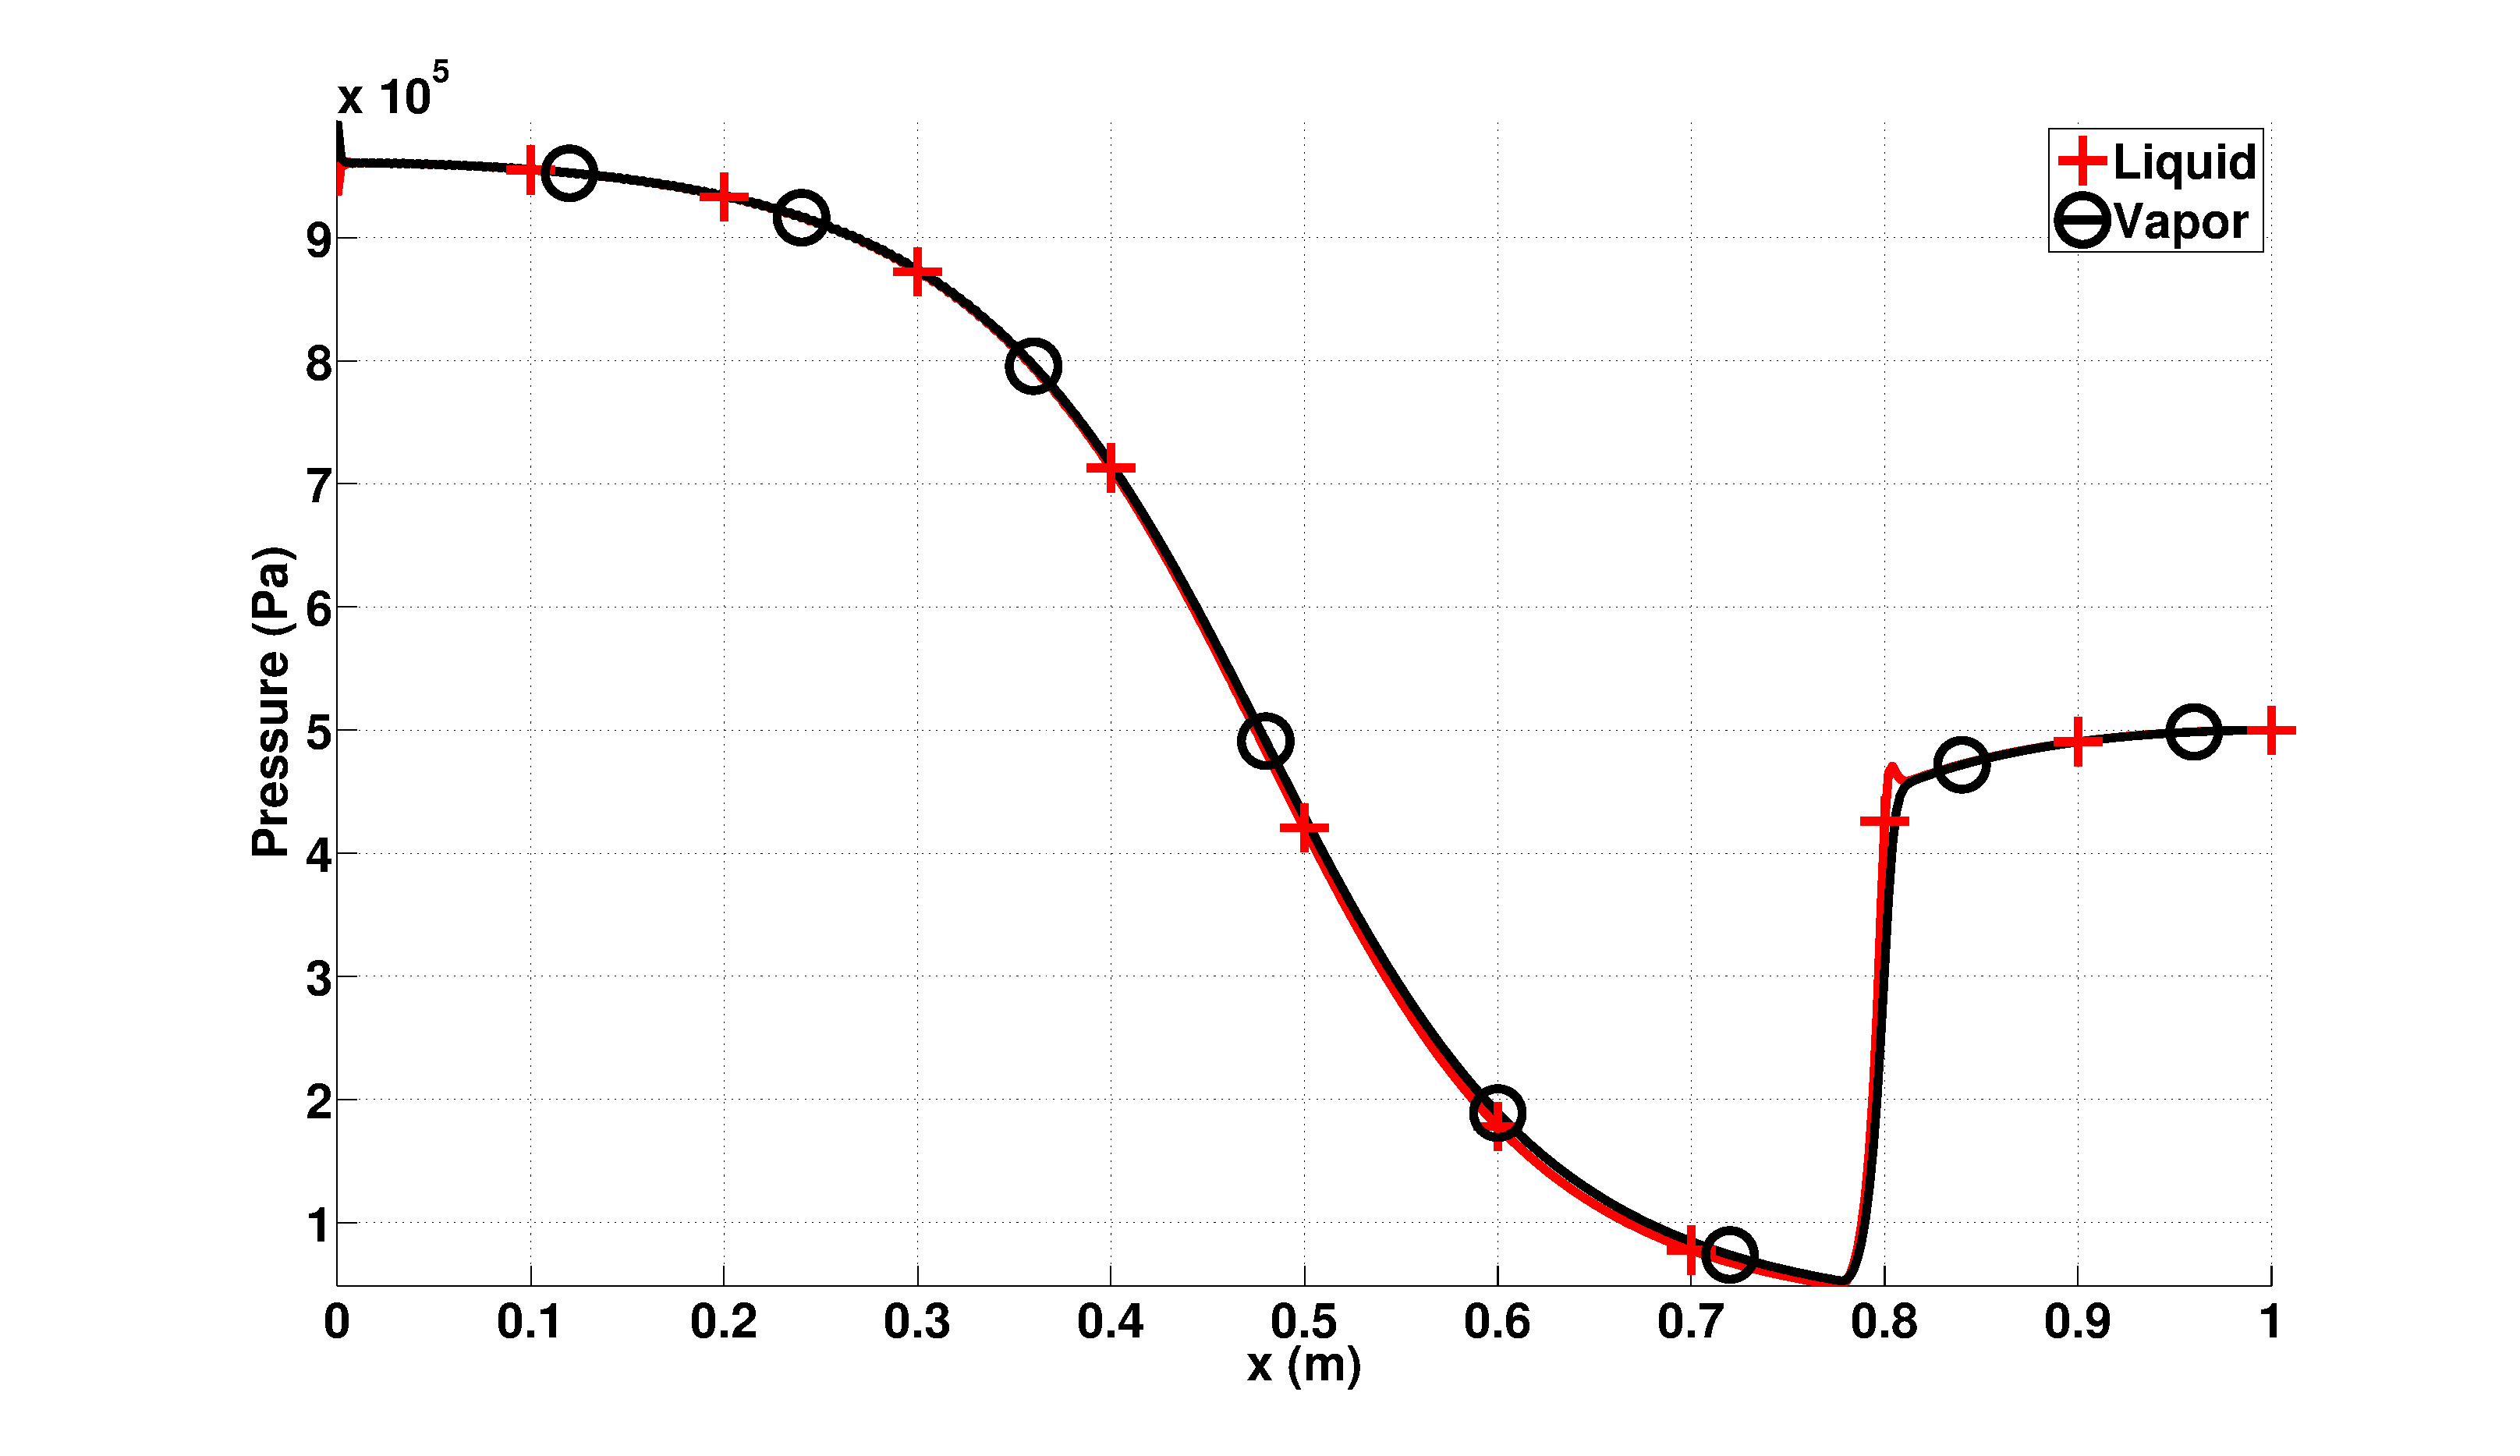
\includegraphics[width=\textwidth]{figures/nozzle-aint-1e4_two_phases_pressure.eps}
                \caption{Pressure}
                \label{fig:nozzle-aint-1e4-press}
        \end{subfigure}        
        \begin{subfigure}[b]{0.495\textwidth}
                \centering
                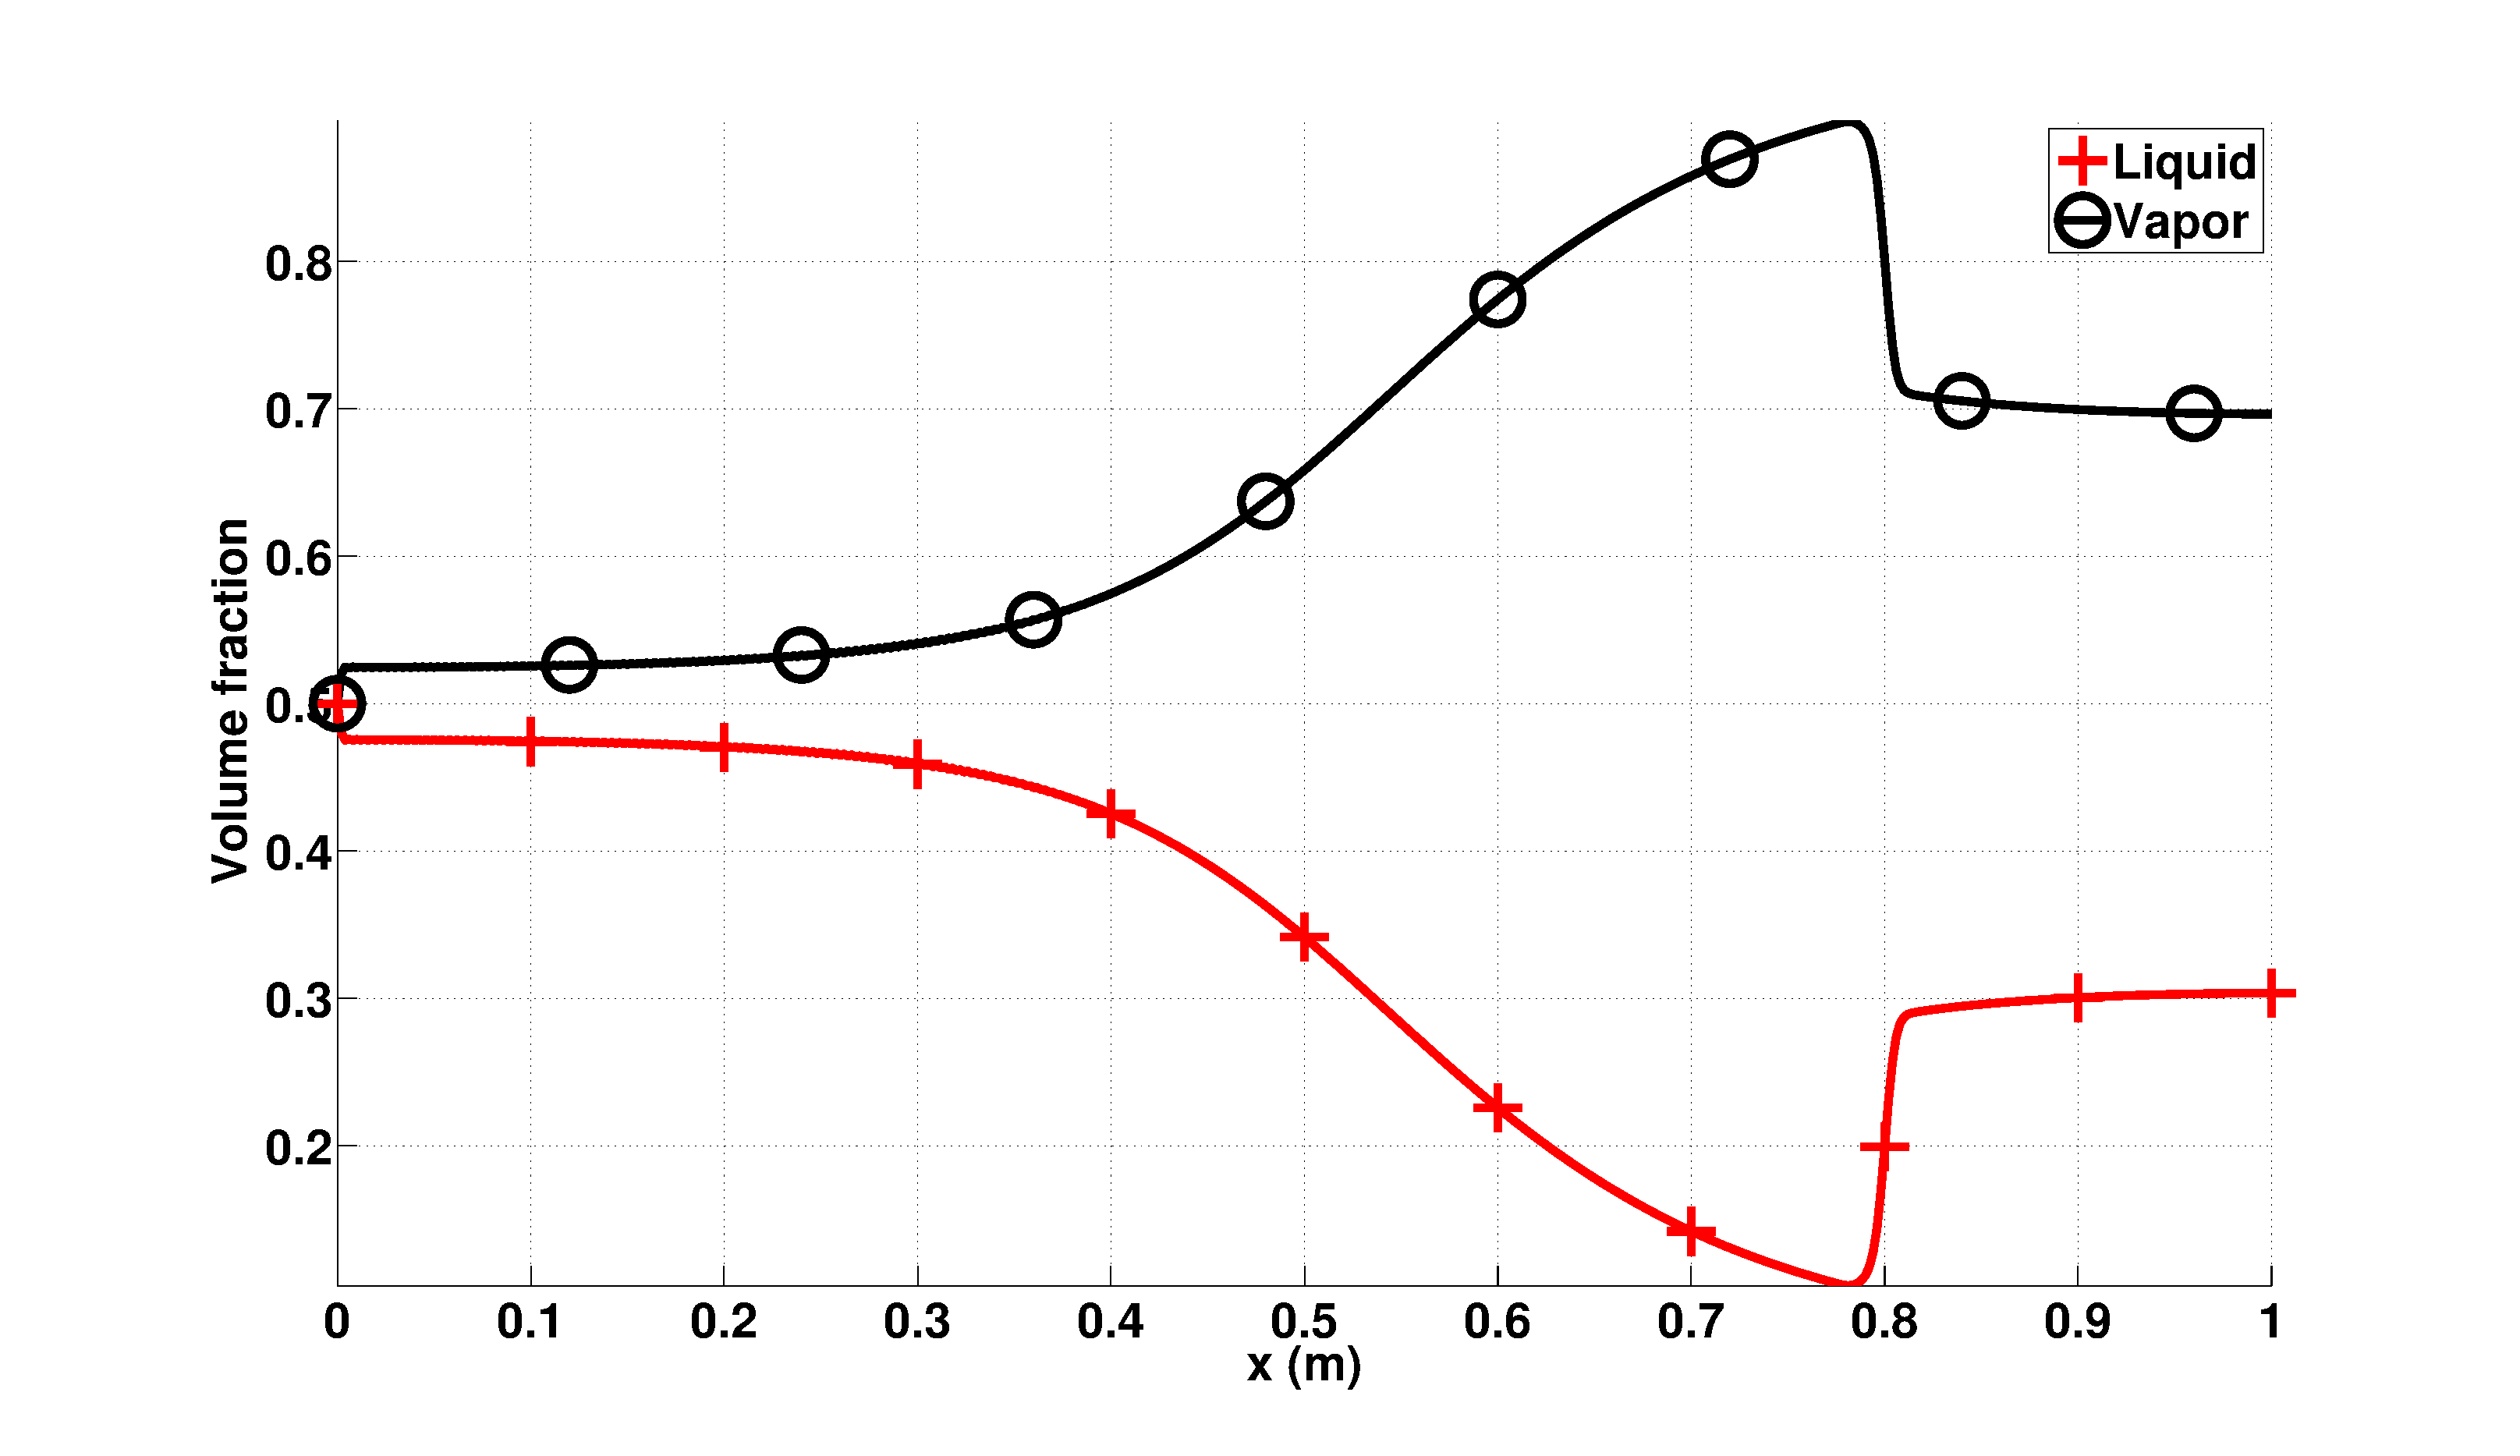
\includegraphics[width=\textwidth]{figures/nozzle-aint-1e4_two_phases_volume_fraction.eps}
                \caption{Volume fraction}
                \label{fig:nozzle-aint-1e4-vf}
        \end{subfigure}
        \caption{Numerical steady-state solution of a two-phase flow in a $1$-D converging-diverging nozzle with infinite relaxation coefficients.}\label{fig:nozzle-aint-1e4-variables}
\end{figure}
%
Because of the velocity relaxation source terms, velocity equilibrium holds between the liquid and vapor phases. 
The pressure profile is given in \fig{fig:nozzle-aint-1e4-press}. The static pressure outlet boundary holds for both phases. At the inlet, the liquid and vapor pressures are not equal since the implementation of the boundary condition does not account for the relaxation terms: the static pressure is computed from the stagnation pressure using entropy and enthalpy conservation relations. The volume fraction of both phases varies throughout the nozzle as a consequence of the pressure equilibrium. Even if the liquid and vapor phases have the same pressure and velocity profiles, the Mach numbers are still very different as shown in FIGURES: the liquid and vapor phases experience a low-Mach and transonic flows, respectively. Consequently, the scaling of the phasic viscosity coefficients and more particularly the normalization parameters will be affected as shown in \fig{fig:nozzle-aint-1e4-visc-coeff}.
%
\begin{figure}[H]
        \centering
        \begin{subfigure}[b]{0.495\textwidth}
                \centering
                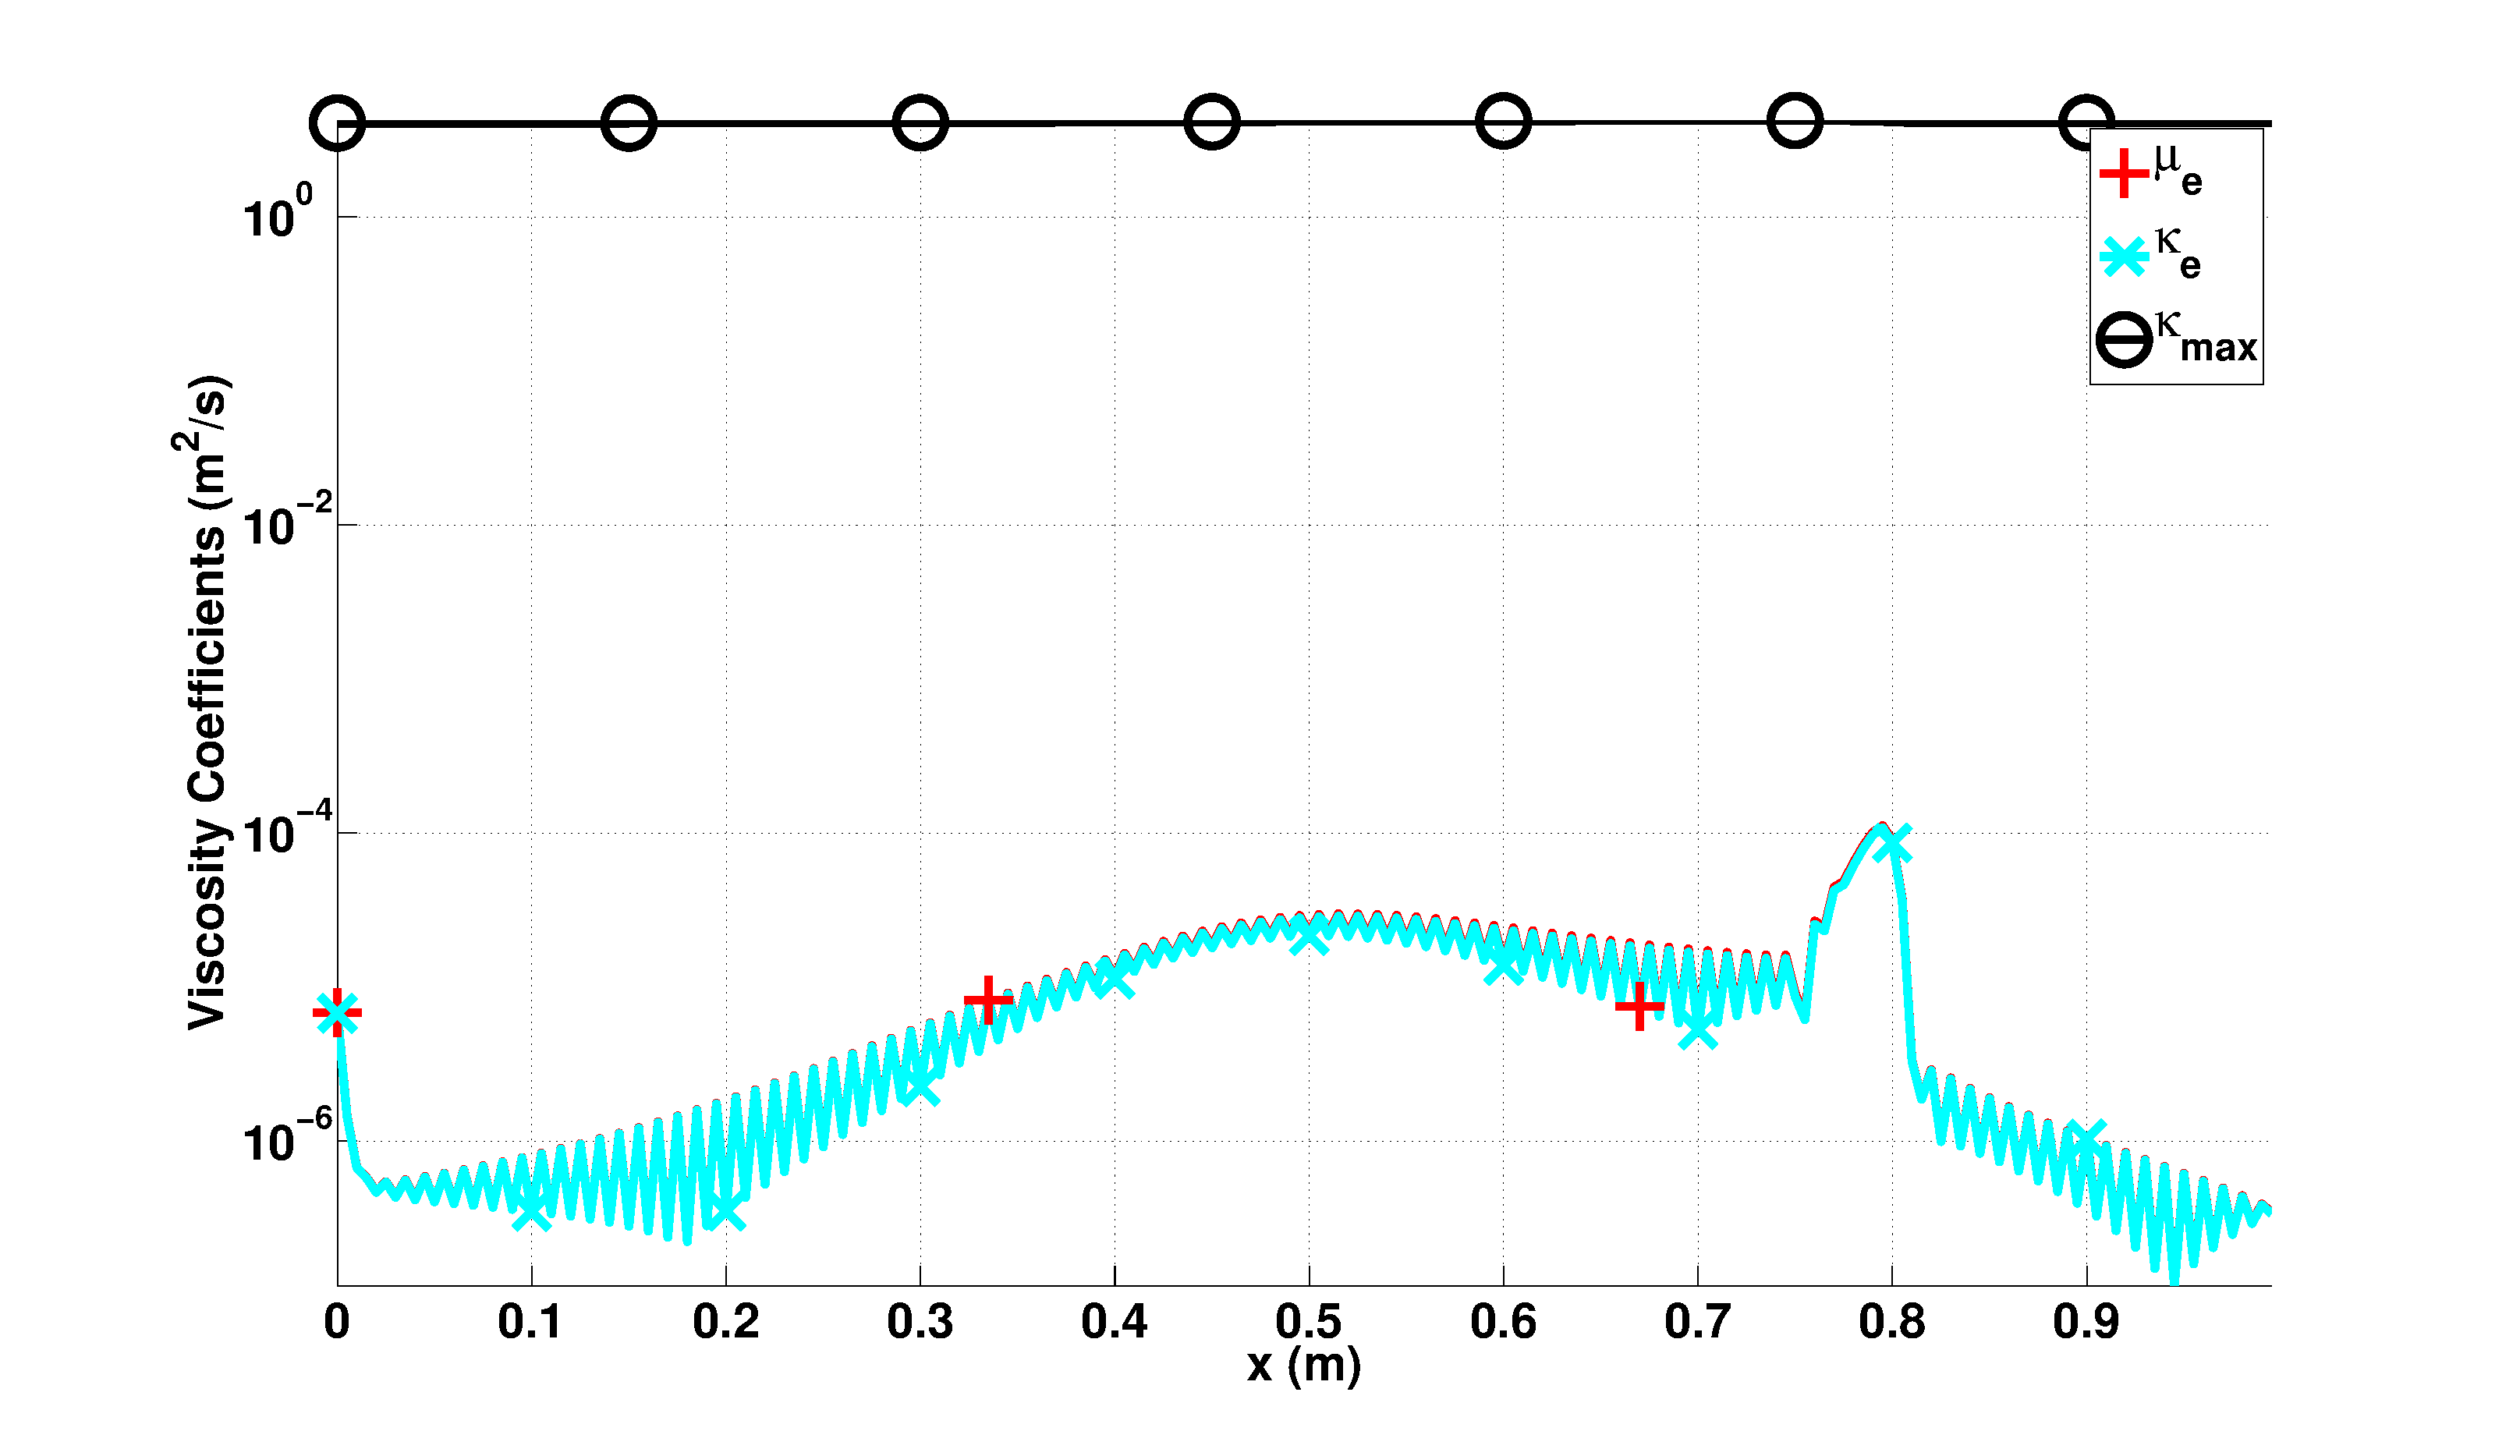
\includegraphics[width=\textwidth]{figures/nozzle-aint-1e4_liquid_viscosity_kappa_mu.eps}
                \caption{Viscosity coefficients for phase 1.}
                \label{fig:nozzle-aint-1e4-visc-coeff-phase-1}
        \end{subfigure}%
        \begin{subfigure}[b]{0.495\textwidth}
                \centering
                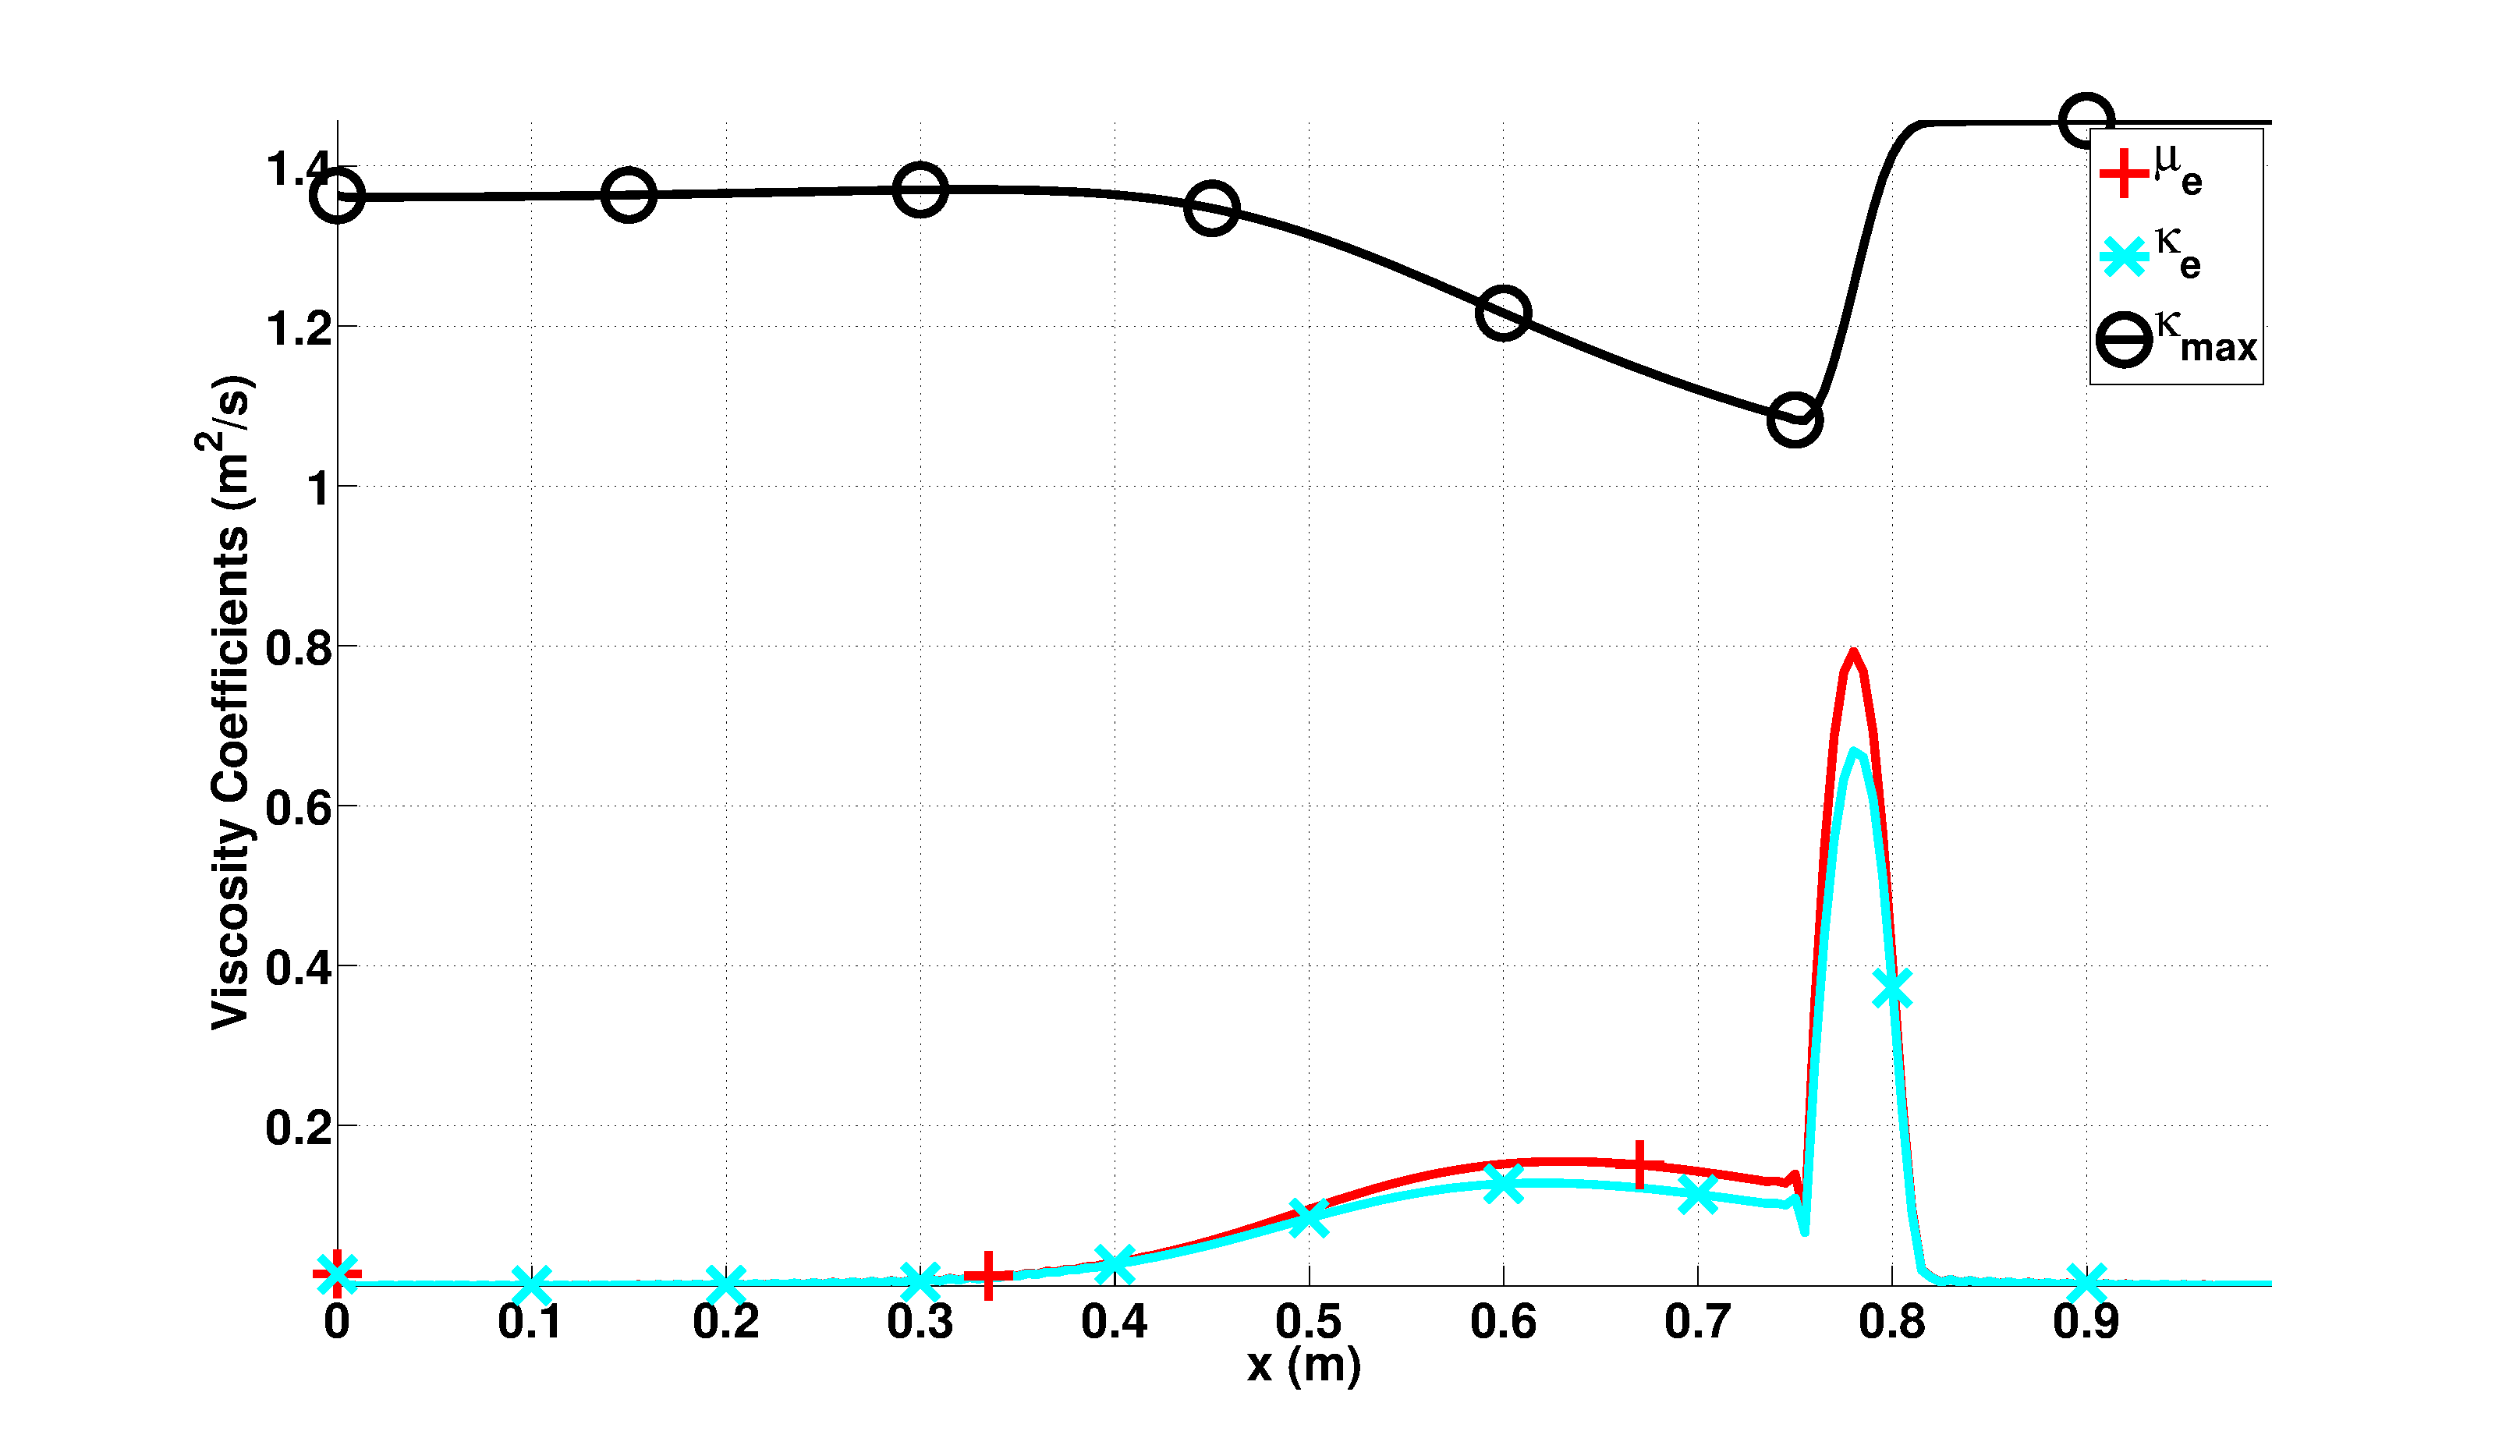
\includegraphics[width=\textwidth]{figures/nozzle-aint-1e4_vapor_viscosity_kappa_mu.eps}
                \caption{Viscosity coefficients for phase 2}
                \label{fig:nozzle-aint-1e4-visc-coeff-phase-2}
        \end{subfigure}
        
        \begin{subfigure}[b]{0.495\textwidth}
                \centering
                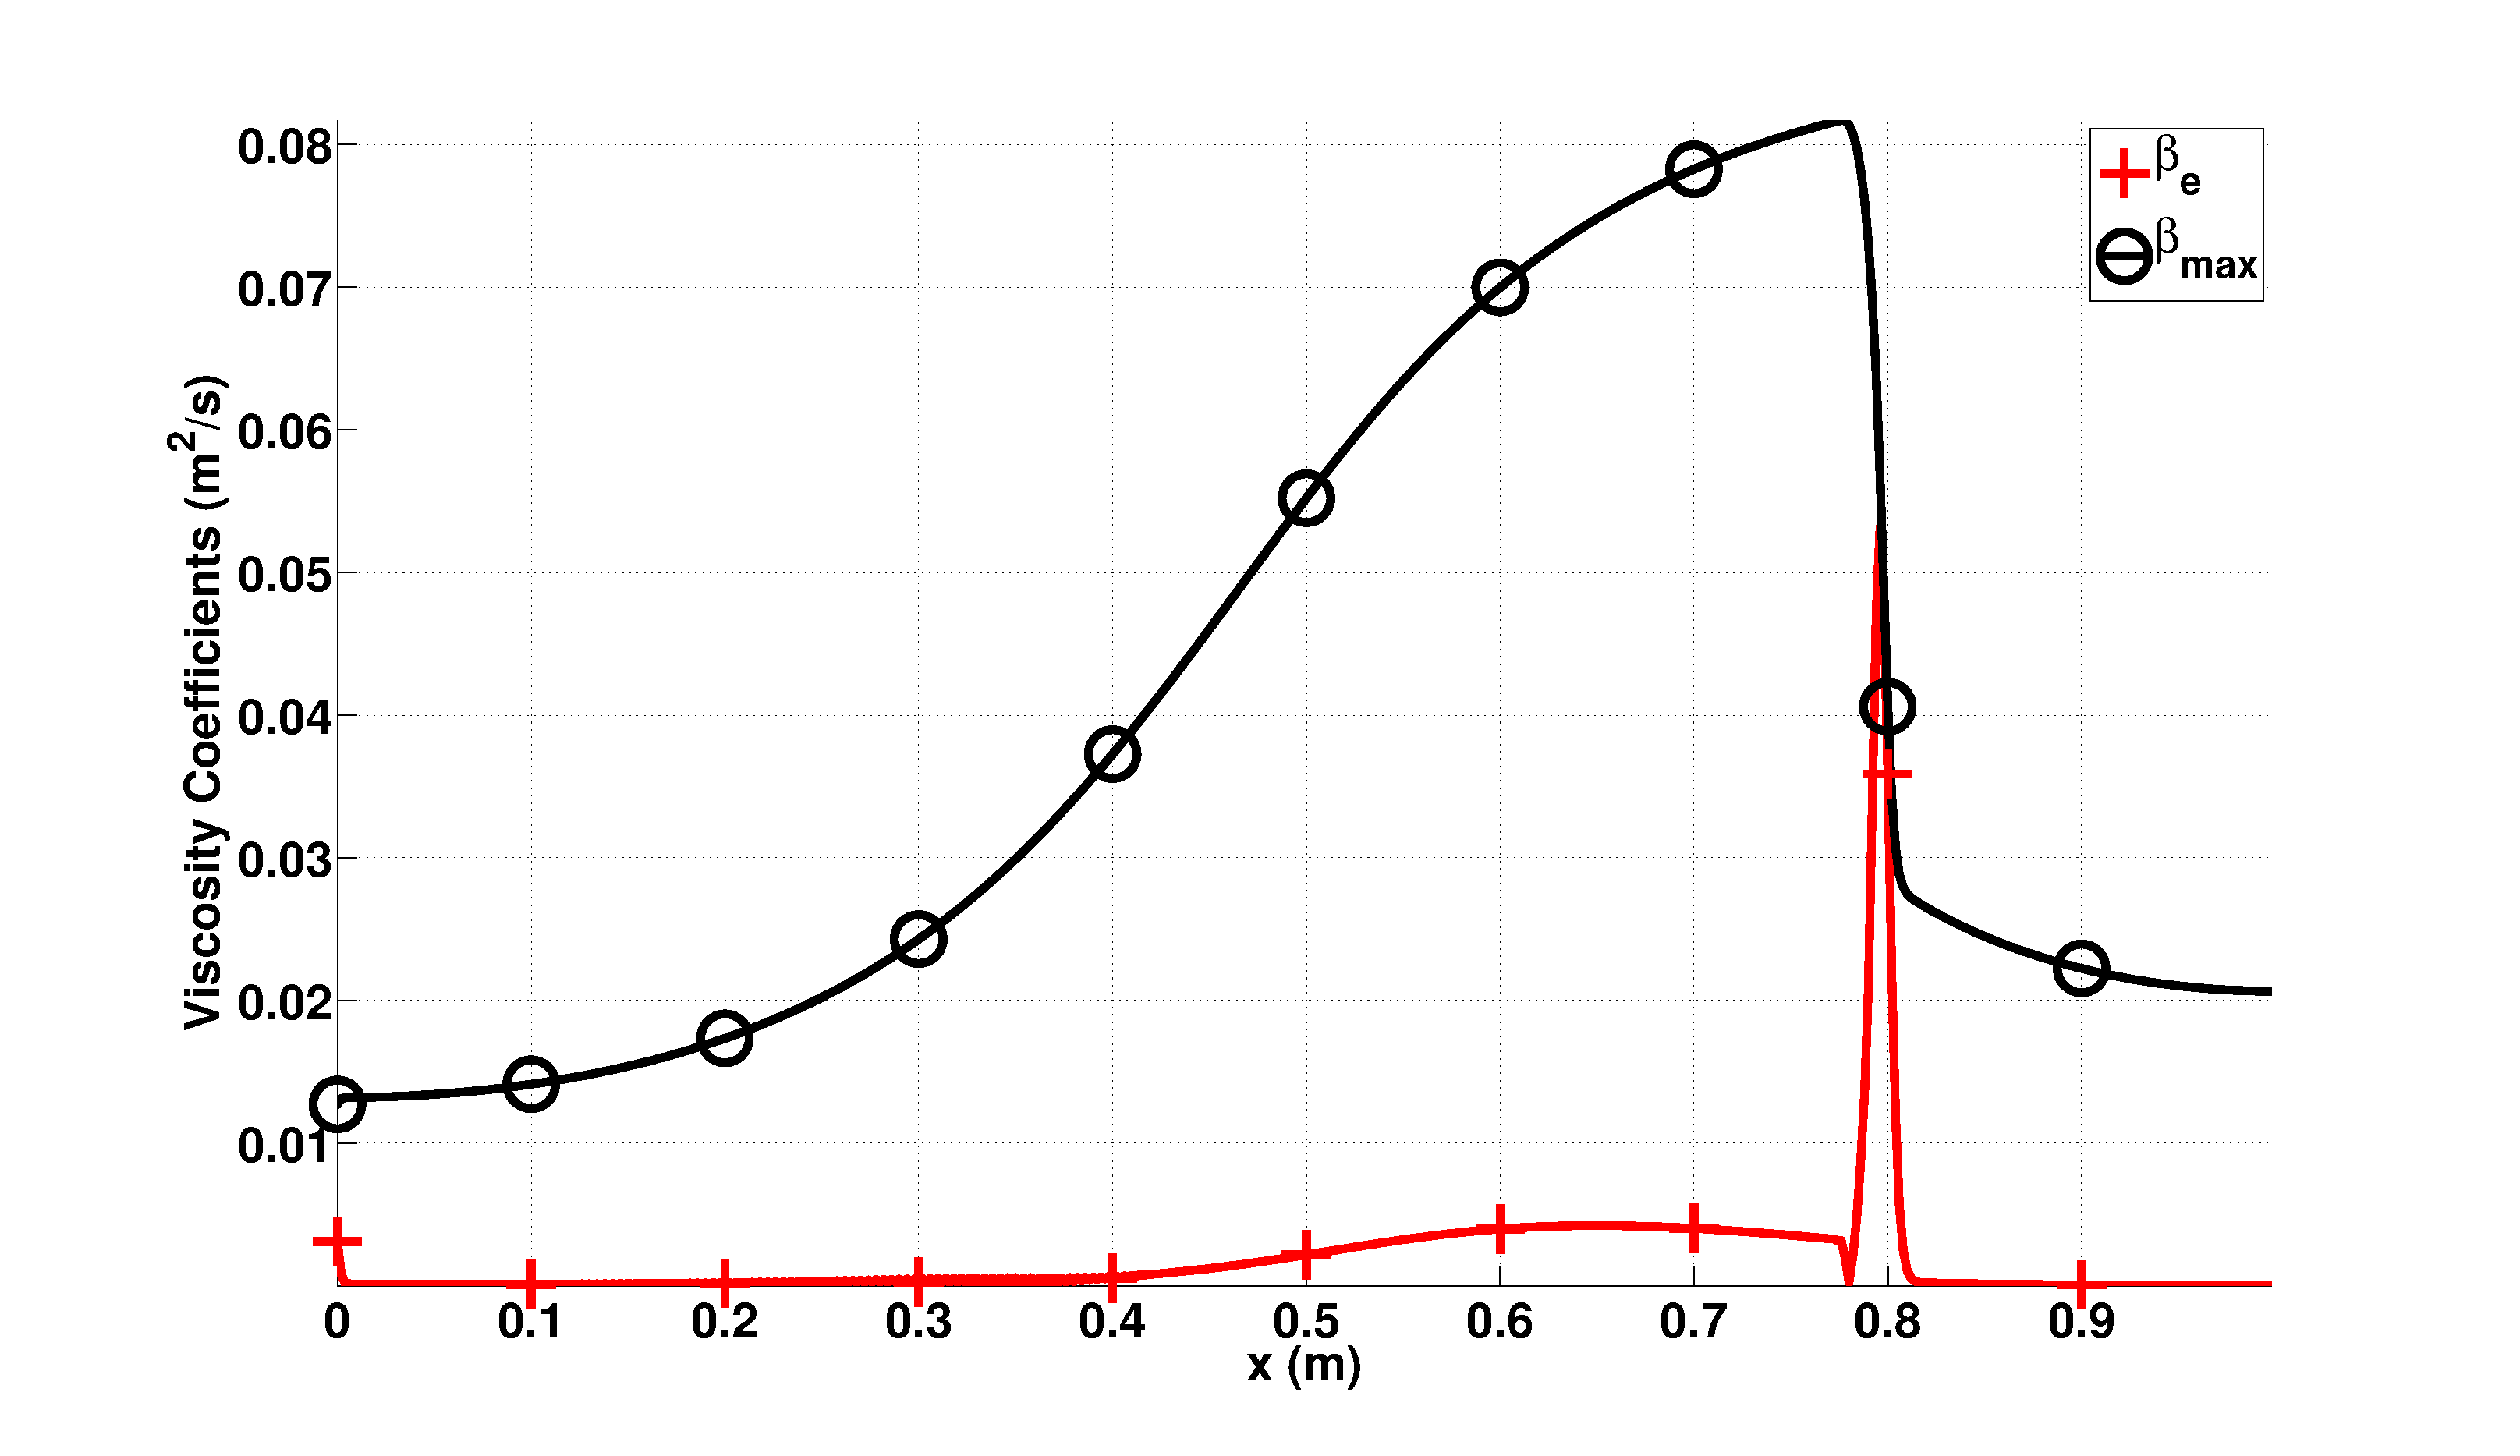
\includegraphics[width=\textwidth]{figures/nozzle-aint-1e4_liquid_beta.eps}
                \caption{Viscosity coefficients for the volume fraction equation of phase 1.}
                \label{fig:nozzle-aint-1e4-beta}
        \end{subfigure}        
        \caption{Viscosity coefficients profiles for a two-phase flow with large relaxation coefficients at $t=305 \ \mu s$.}\label{fig:nozzle-aint-1e4-visc-coeff}
\end{figure}
%
The phasic viscosity coefficients $\mu_k$ and $\kappa_k$ are peaked in the vicinity of the sharp variation around $x=0.8 \ m$. Lastly, the viscosity coefficient $\beta_k$ follows the variations of the volume fraction for both phases. It is interesting to note that the fast vapor flow yields strong variations in the divergent part of the nozzle. Overall, the viscosity coefficients are large enough to prevent the formation of any numerical instability without altering the physical solution.
%
%%%%%%%%%%%%%%%%%%%%%%%%%%%%%%%%%%%%%
\subsection{1-D numerical results obtained with Relap-7}\label{sec:1d-results-relap-7}
%%%%%%%%%%%%%%%%%%%%%%%%%%%%%%%%%%%%%
%
We now present results of typical engineering problems obtained with the system code RELAP-7 \cite{Berry_2014} with the objective of testing adequacy of the Entropy Viscosity Method when computing typical reactor flows: a hydrostatic test, a two-phase flow water-hammer and a Boiling Water Reactor (BWR). 
%The numerical results were obtained with the system code RELAP-7 that implements the single- and two-phase flow models described in \sct{sct:model} using the spatial and temporal discretization techniques \sct{sec:spatial-disc} (BDF2 and linear test functions).
%
%%%%%%%%%%%%%%%%%%%%%%%%%%%%%%%%%%%%%
\subsubsection{A two-phase flow water hammer test}\label{sec:water-hammer}
%%%%%%%%%%%%%%%%%%%%%%%%%%%%%%%%%%%%%
%
A water-hammer situation is encountered in light water reactors whenever a valve closes rapidly and obstructs the flow in a pipe. In the numerical results presented in this section, each fluid is described by the Stiffened Gas equation of state with parameters taken from \tbl{tbl:stff_gas_eos-sect4} for the liquid and gas phases. 
A water hammer consists of a liquid phase flowing in a straight 1-D pipe of length $L=10 \ m$ with initial uniform pressure ($P = 7$ MPa), velocity ($u = -12$ $m/s$) and temperature ($T = 453$ K). At $t=0$ s, the two extremities of the 1-D pipe are closed by solid walls which causes shock and rarefaction waves to appear at the left and right extremities, respectively. The two waves initially propagate towards the middle of the pipe and are reflected on the opposite wall after crossing each other near the middle of the pipe.
The liquid and vapor phases have the same initial conditions and the liquid volume fraction is initially set to $0.5$. The two phases are in interaction through the pressure and velocity relaxation terms that are functions of the relaxation coefficients, $\mu_P$ and $\lambda_u$, computed with $A_{int} = 10^3$ $m^{-1}$ so that the two phases achieve pressure and velocity equilibrium at all times.
The computational domain is discretized with an uniform mesh of $500$ cells and the numerical solution is run until $t = 0.5$ s with a CFL number of $1.$ for both tests. Information regarding the initial conditions will be given later in this section. 
For each test case, the velocity, density and pressure profiles are provided at different times of the simulation. Plots of the velocity, the density, the pressure are given in \fig{fig:water-hammer-var}. The corresponding phasic viscosity coefficients are shown in \fig{fig:water-hammer-visc}.
%
\begin{figure}[H]
        \centering
        \begin{subfigure}[b]{0.495\textwidth}
                \centering
                \includegraphics[width=\textwidth]{figures/water-hammer-density-liquid.eps}
                \caption{Liquid density}
                \label{fig:water-hammer-density-liq}
        \end{subfigure}%
        \begin{subfigure}[b]{0.495\textwidth}
                \centering
                \includegraphics[width=\textwidth]{figures/water-hammer-density-vapor.eps}
                \caption{Vapor density}
                \label{fig:water-hammer-density-vap}
        \end{subfigure}
        
        \begin{subfigure}[b]{0.495\textwidth}
                \centering
                \includegraphics[width=\textwidth]{figures/water-hammer-pressure-liquid.eps}
                \caption{Pressure}
                \label{fig:water-hammer-press-liq}
        \end{subfigure}        
        \begin{subfigure}[b]{0.495\textwidth}
                \centering
                \includegraphics[width=\textwidth]{figures/water-hammer-pressure-vapor.eps}
                \caption{Volume fraction}
                \label{fig:water-hammer-press-vap}
        \end{subfigure}
        \caption{Numerical solution of a two-phase flow with large relaxation coefficients at $t=305 \ \mu s$.}\label{fig:water-hammer-var}
\end{figure}
%
\fig{fig:water-hammer-var} show that the numerical solution of the liquid and gas phases do not display any oscillations or instabilities. 
As expected, the two fluids have the same pressure and velocity profiles as shown in FIGURES, respectively. The shocks coming from the left and right walls are initially well resolved and do not display any instability. The density of the liquid and gas phases have different values but experience similar variations. It is also noted that the accuracy of the shock wave decreases over time: the numerical dissipation comes from the temporal integrator (time step size) and the spatial discretize element size. The accuracy of the numerical solution could be improved over time by using a finer grid with smaller time steps or a higher-order temporal integrator.
%
\begin{figure}[H]
        \centering
        \begin{subfigure}[b]{0.495\textwidth}
                \centering
                \includegraphics[width=\textwidth]{figures/water-hammer-viscosity-liquid.eps}
                \caption{Viscosity coefficients for phase 1.}
                \label{fig:water-hammer-visc-liq}
        \end{subfigure}%
        \begin{subfigure}[b]{0.495\textwidth}
                \centering
                \includegraphics[width=\textwidth]{figures/water-hammer-viscosity-vapor.eps}
                \caption{Viscosity coefficients for phase 2}
                \label{fig:water-hammer-visc-vap}
        \end{subfigure}
        
%        \begin{subfigure}[b]{0.495\textwidth}
%                \centering
%                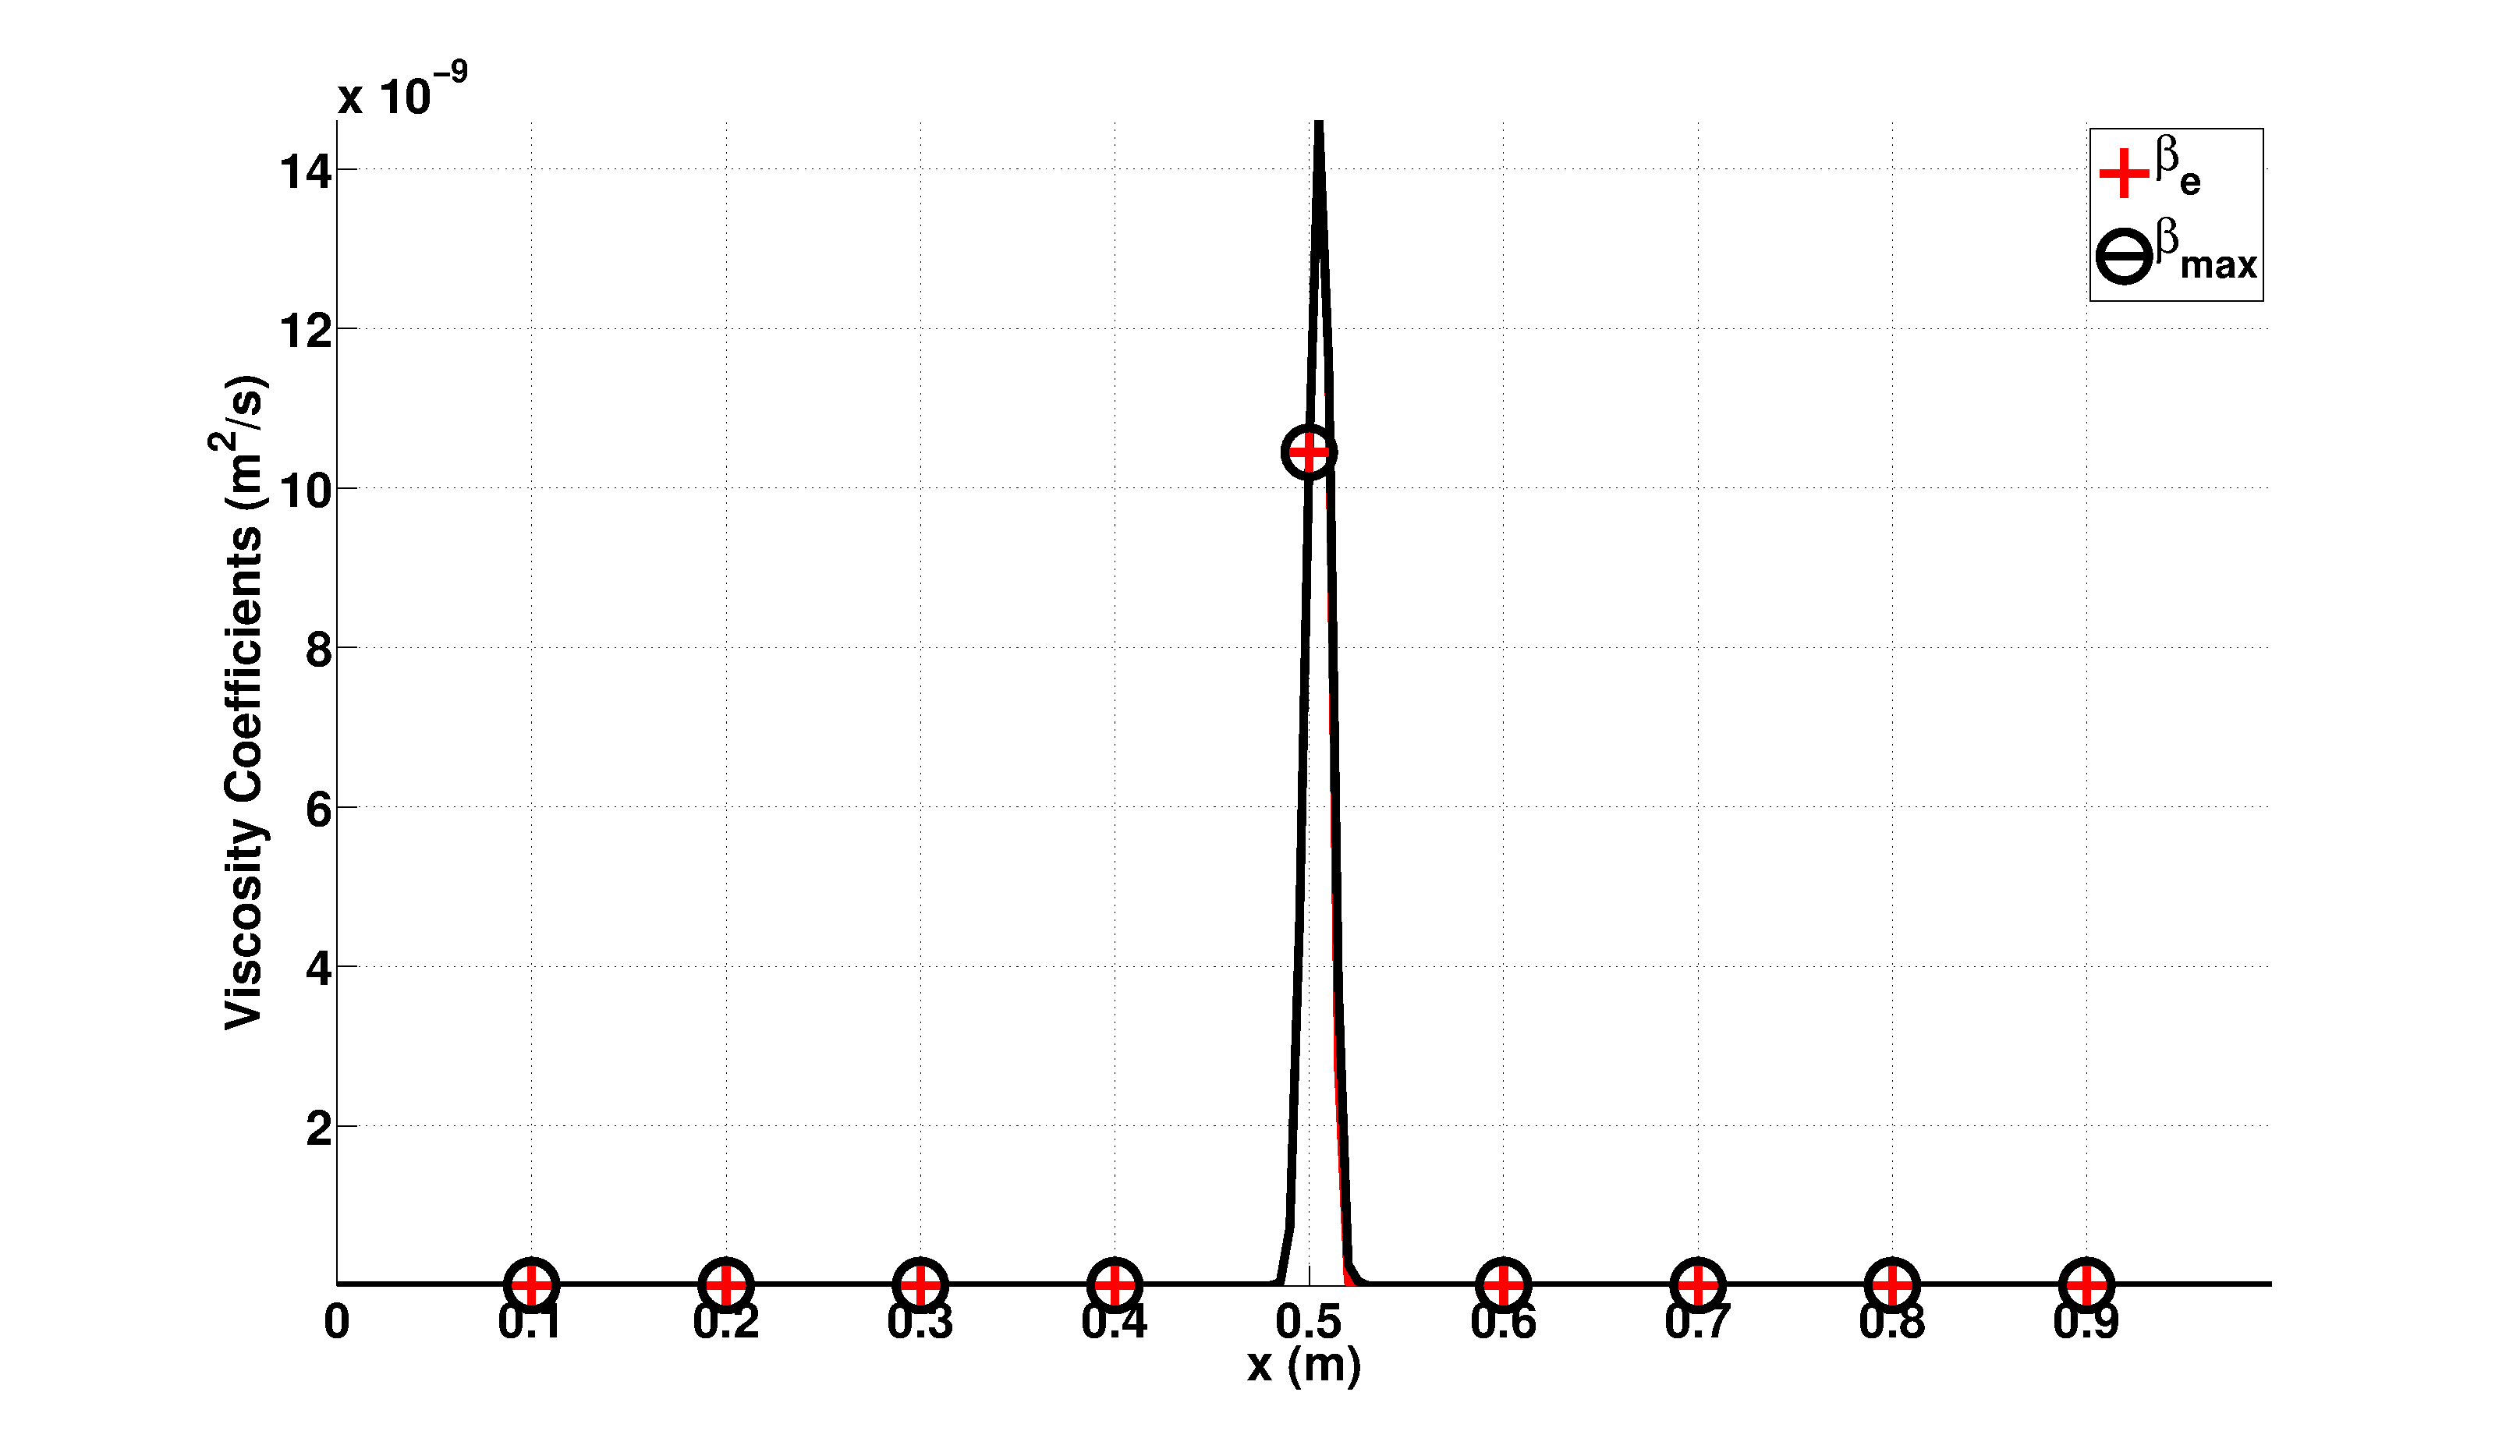
\includegraphics[width=\textwidth]{figures/hydrostatic-_liquid_beta.eps}
%                \caption{Viscosity coefficients for the volume fraction equation of phase 1.}
%                \label{fig:hydrostatic--beta}
%        \end{subfigure}        
        \caption{Viscosity coefficients profiles for a two-phase flow with large relaxation coefficients at $t=305 \ \mu s$.}\label{fig:water-hammer-visc}
\end{figure}
%
The viscosity coefficients are plotted at time $t = 8.7 \times 10^{-3}$ s and display two peaks that match the shock positions.
%
%%%%%%%%%%%%%%%%%%%%%%%%%%%%%%%%%%%%%
\subsubsection{A hydrostatic test}\label{sec:}
%%%%%%%%%%%%%%%%%%%%%%%%%%%%%%%%%%%%%
%
%
\begin{figure}[H]
        \centering
        \begin{subfigure}[b]{0.495\textwidth}
                \centering
                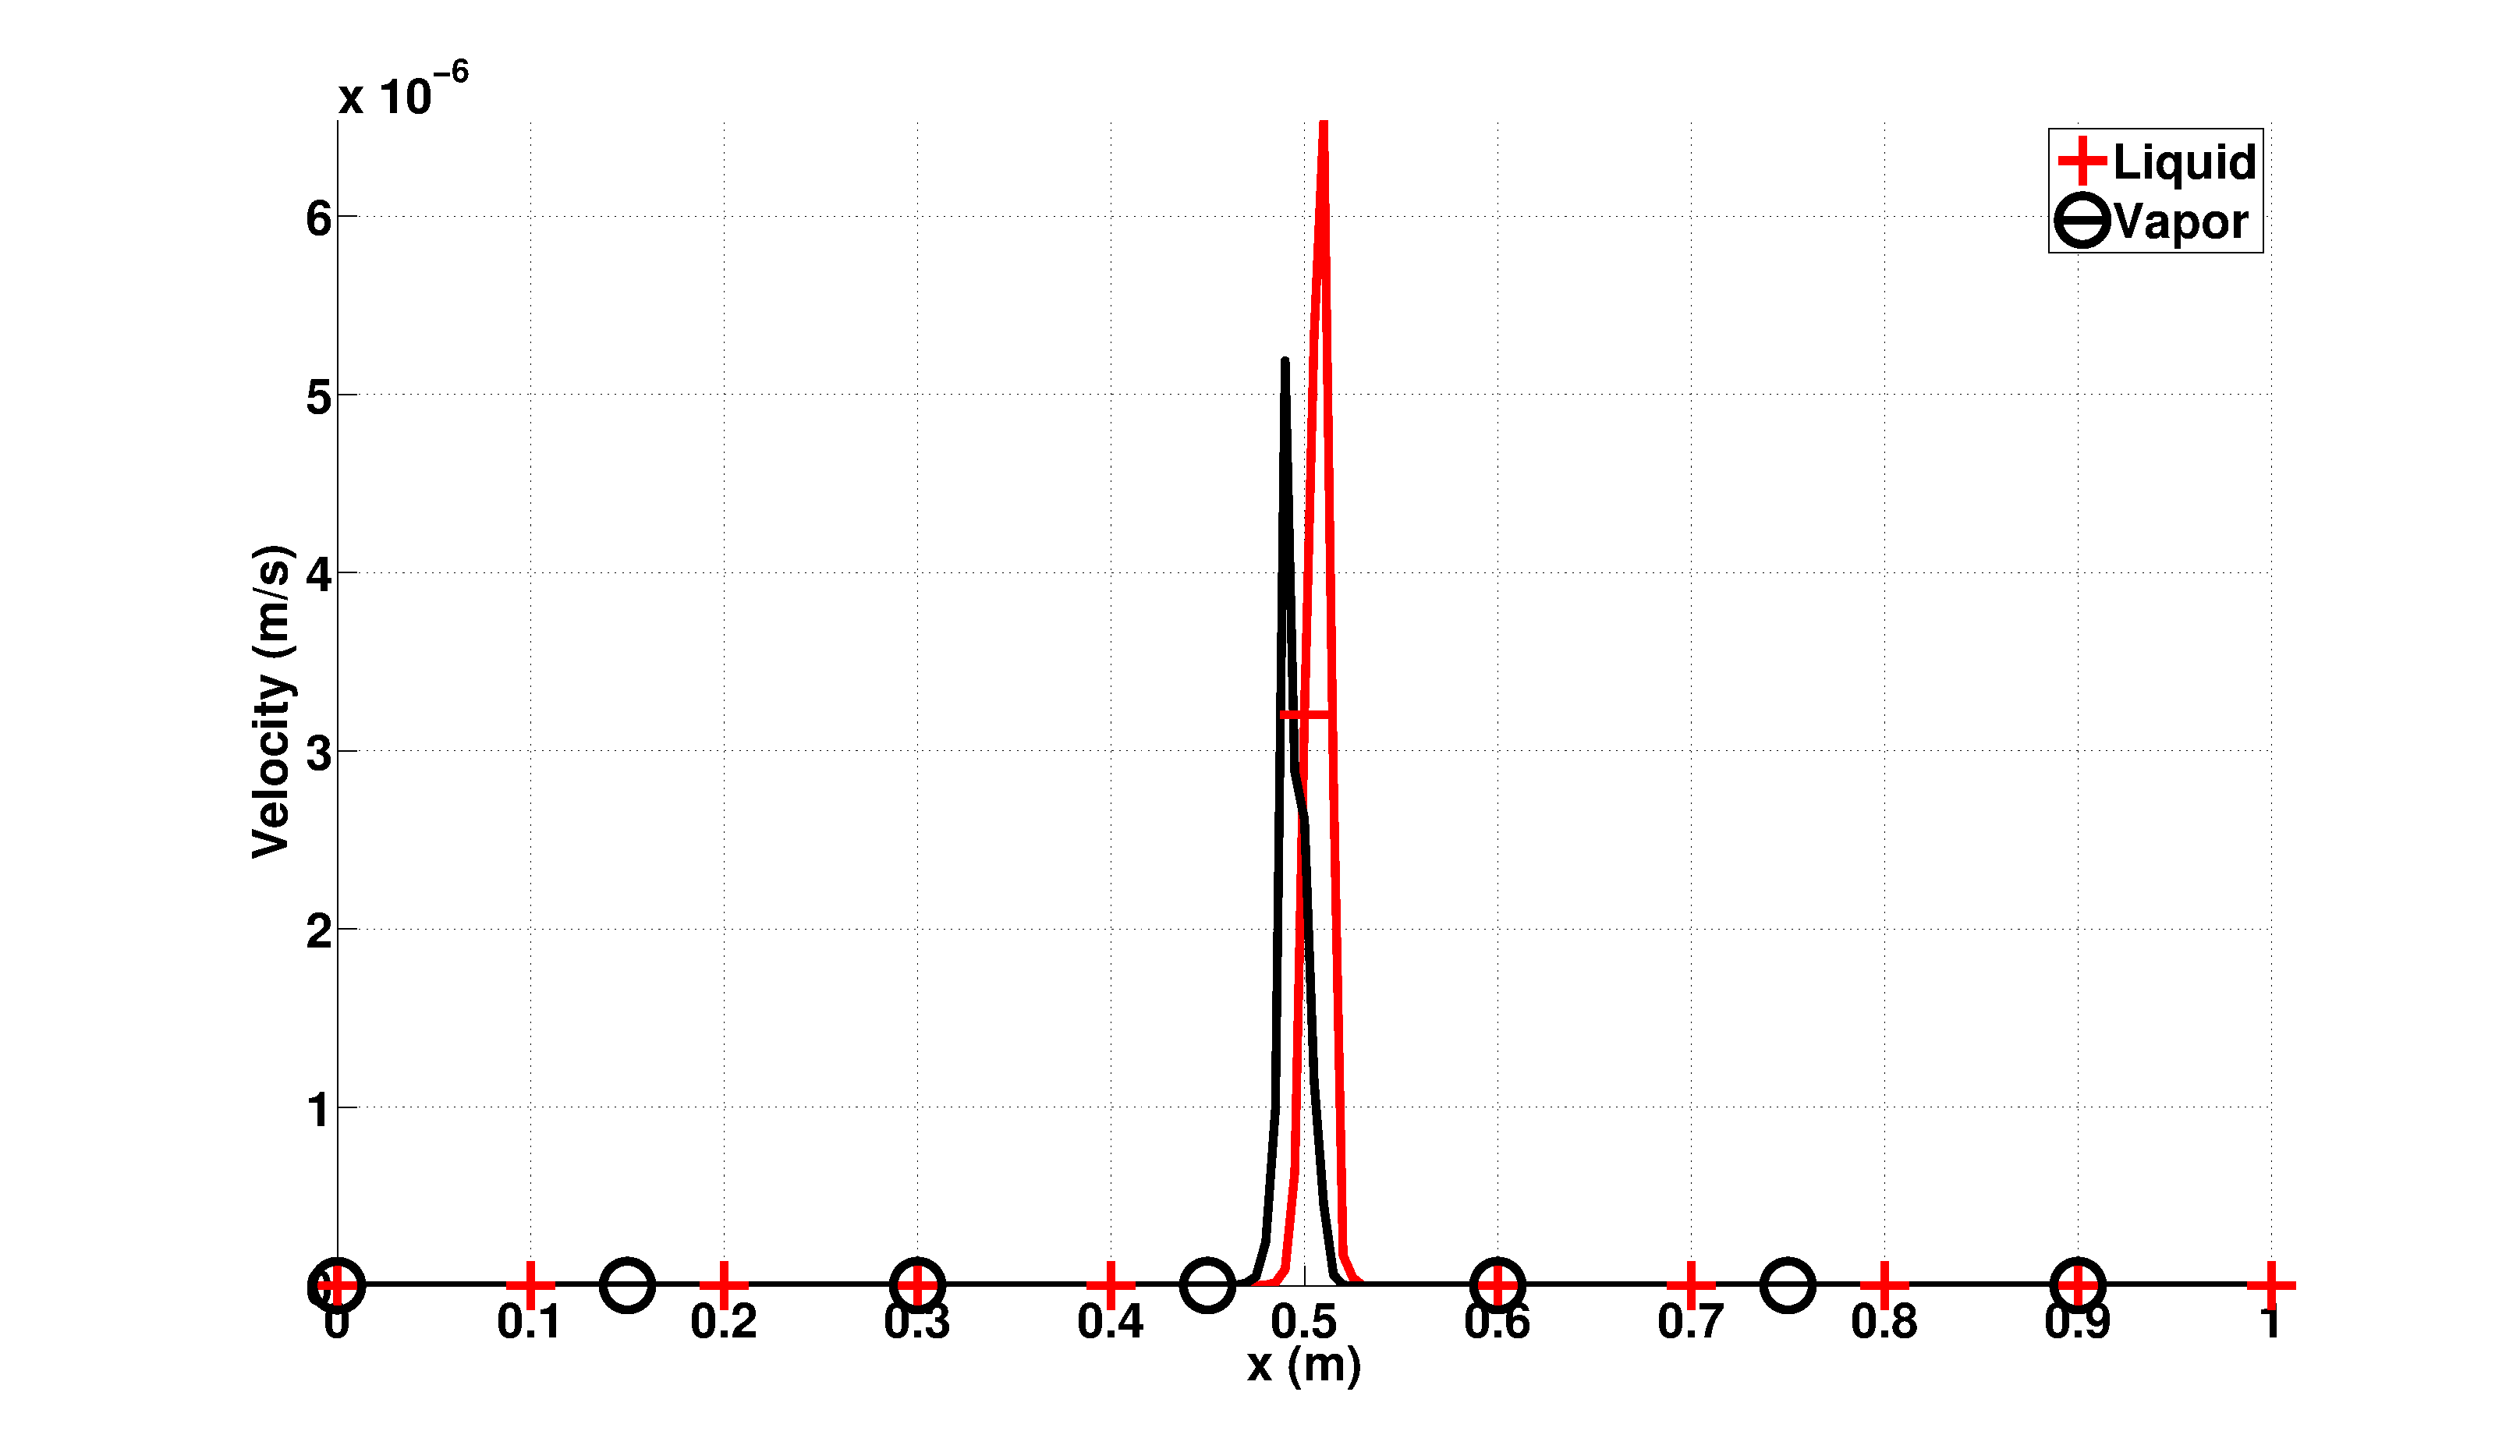
\includegraphics[width=\textwidth]{figures/hydrostatic-_two_phases_velocity.eps}
                \caption{Velocity}
                \label{fig:hydrostatic--vel}
        \end{subfigure}%
        \begin{subfigure}[b]{0.495\textwidth}
                \centering
                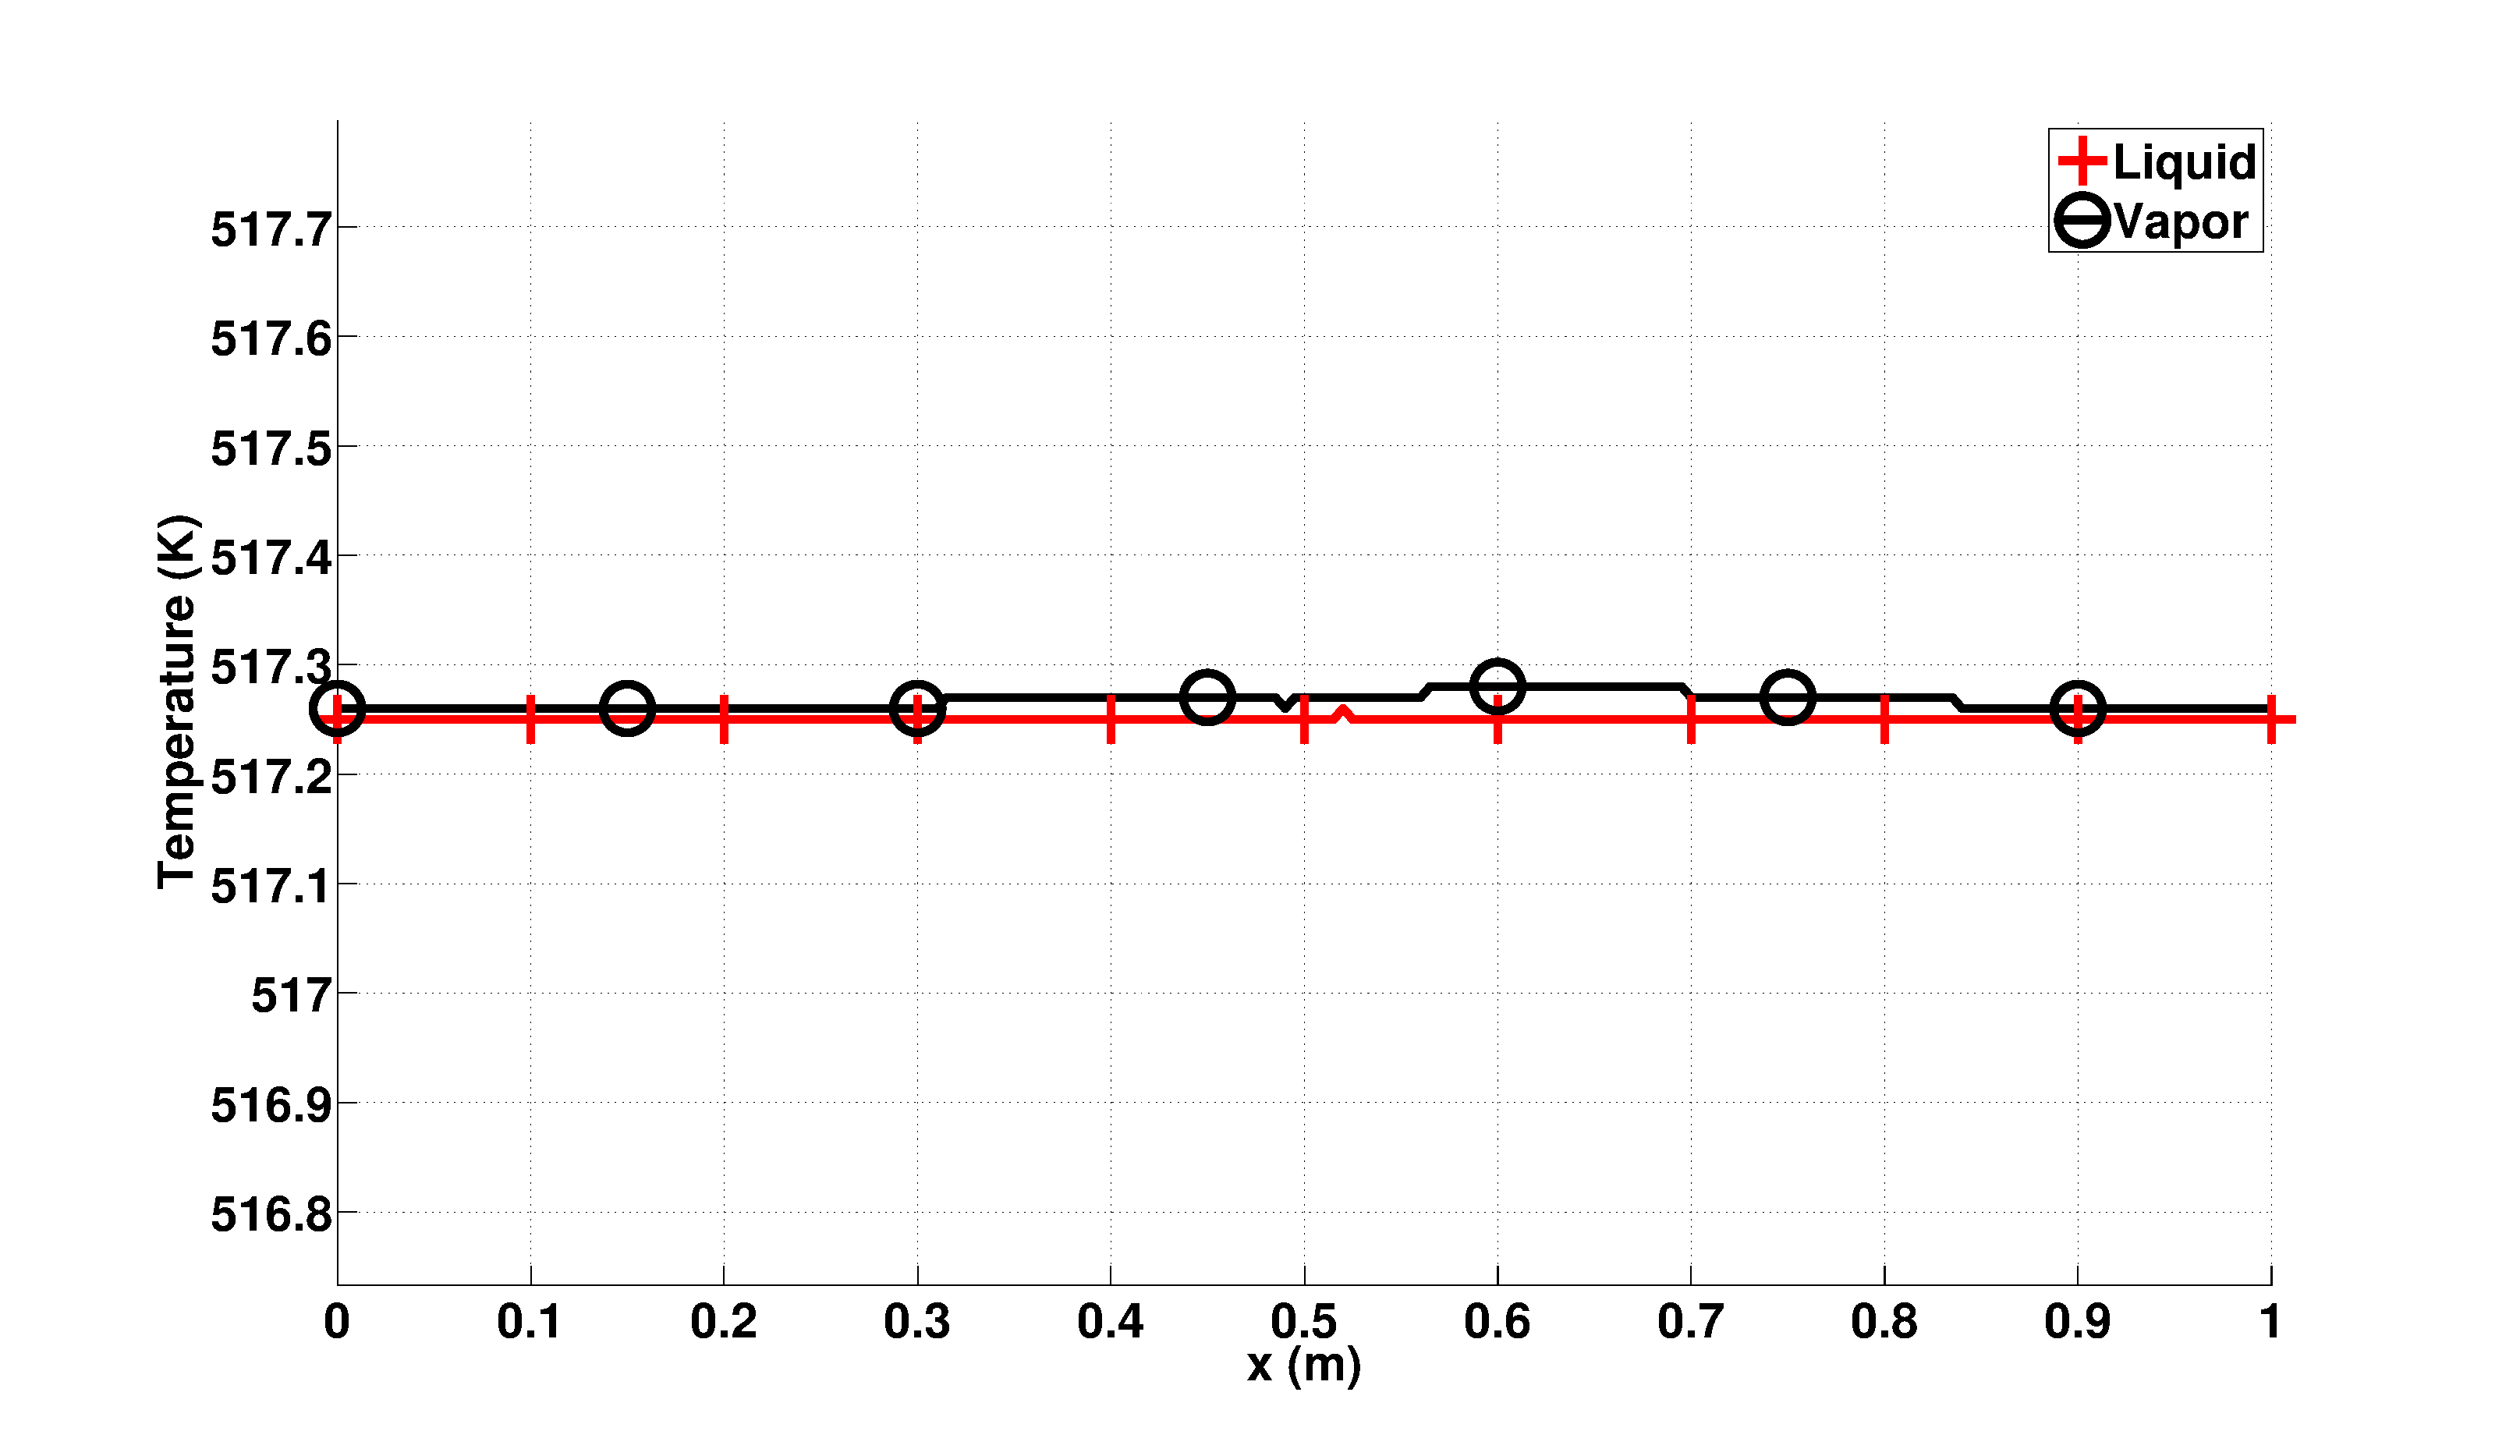
\includegraphics[width=\textwidth]{figures/hydrostatic-_two_phases_temperature.eps}
                \caption{Density}
                \label{fig:hydrostatic--density}
        \end{subfigure}
        
        \begin{subfigure}[b]{0.495\textwidth}
                \centering
                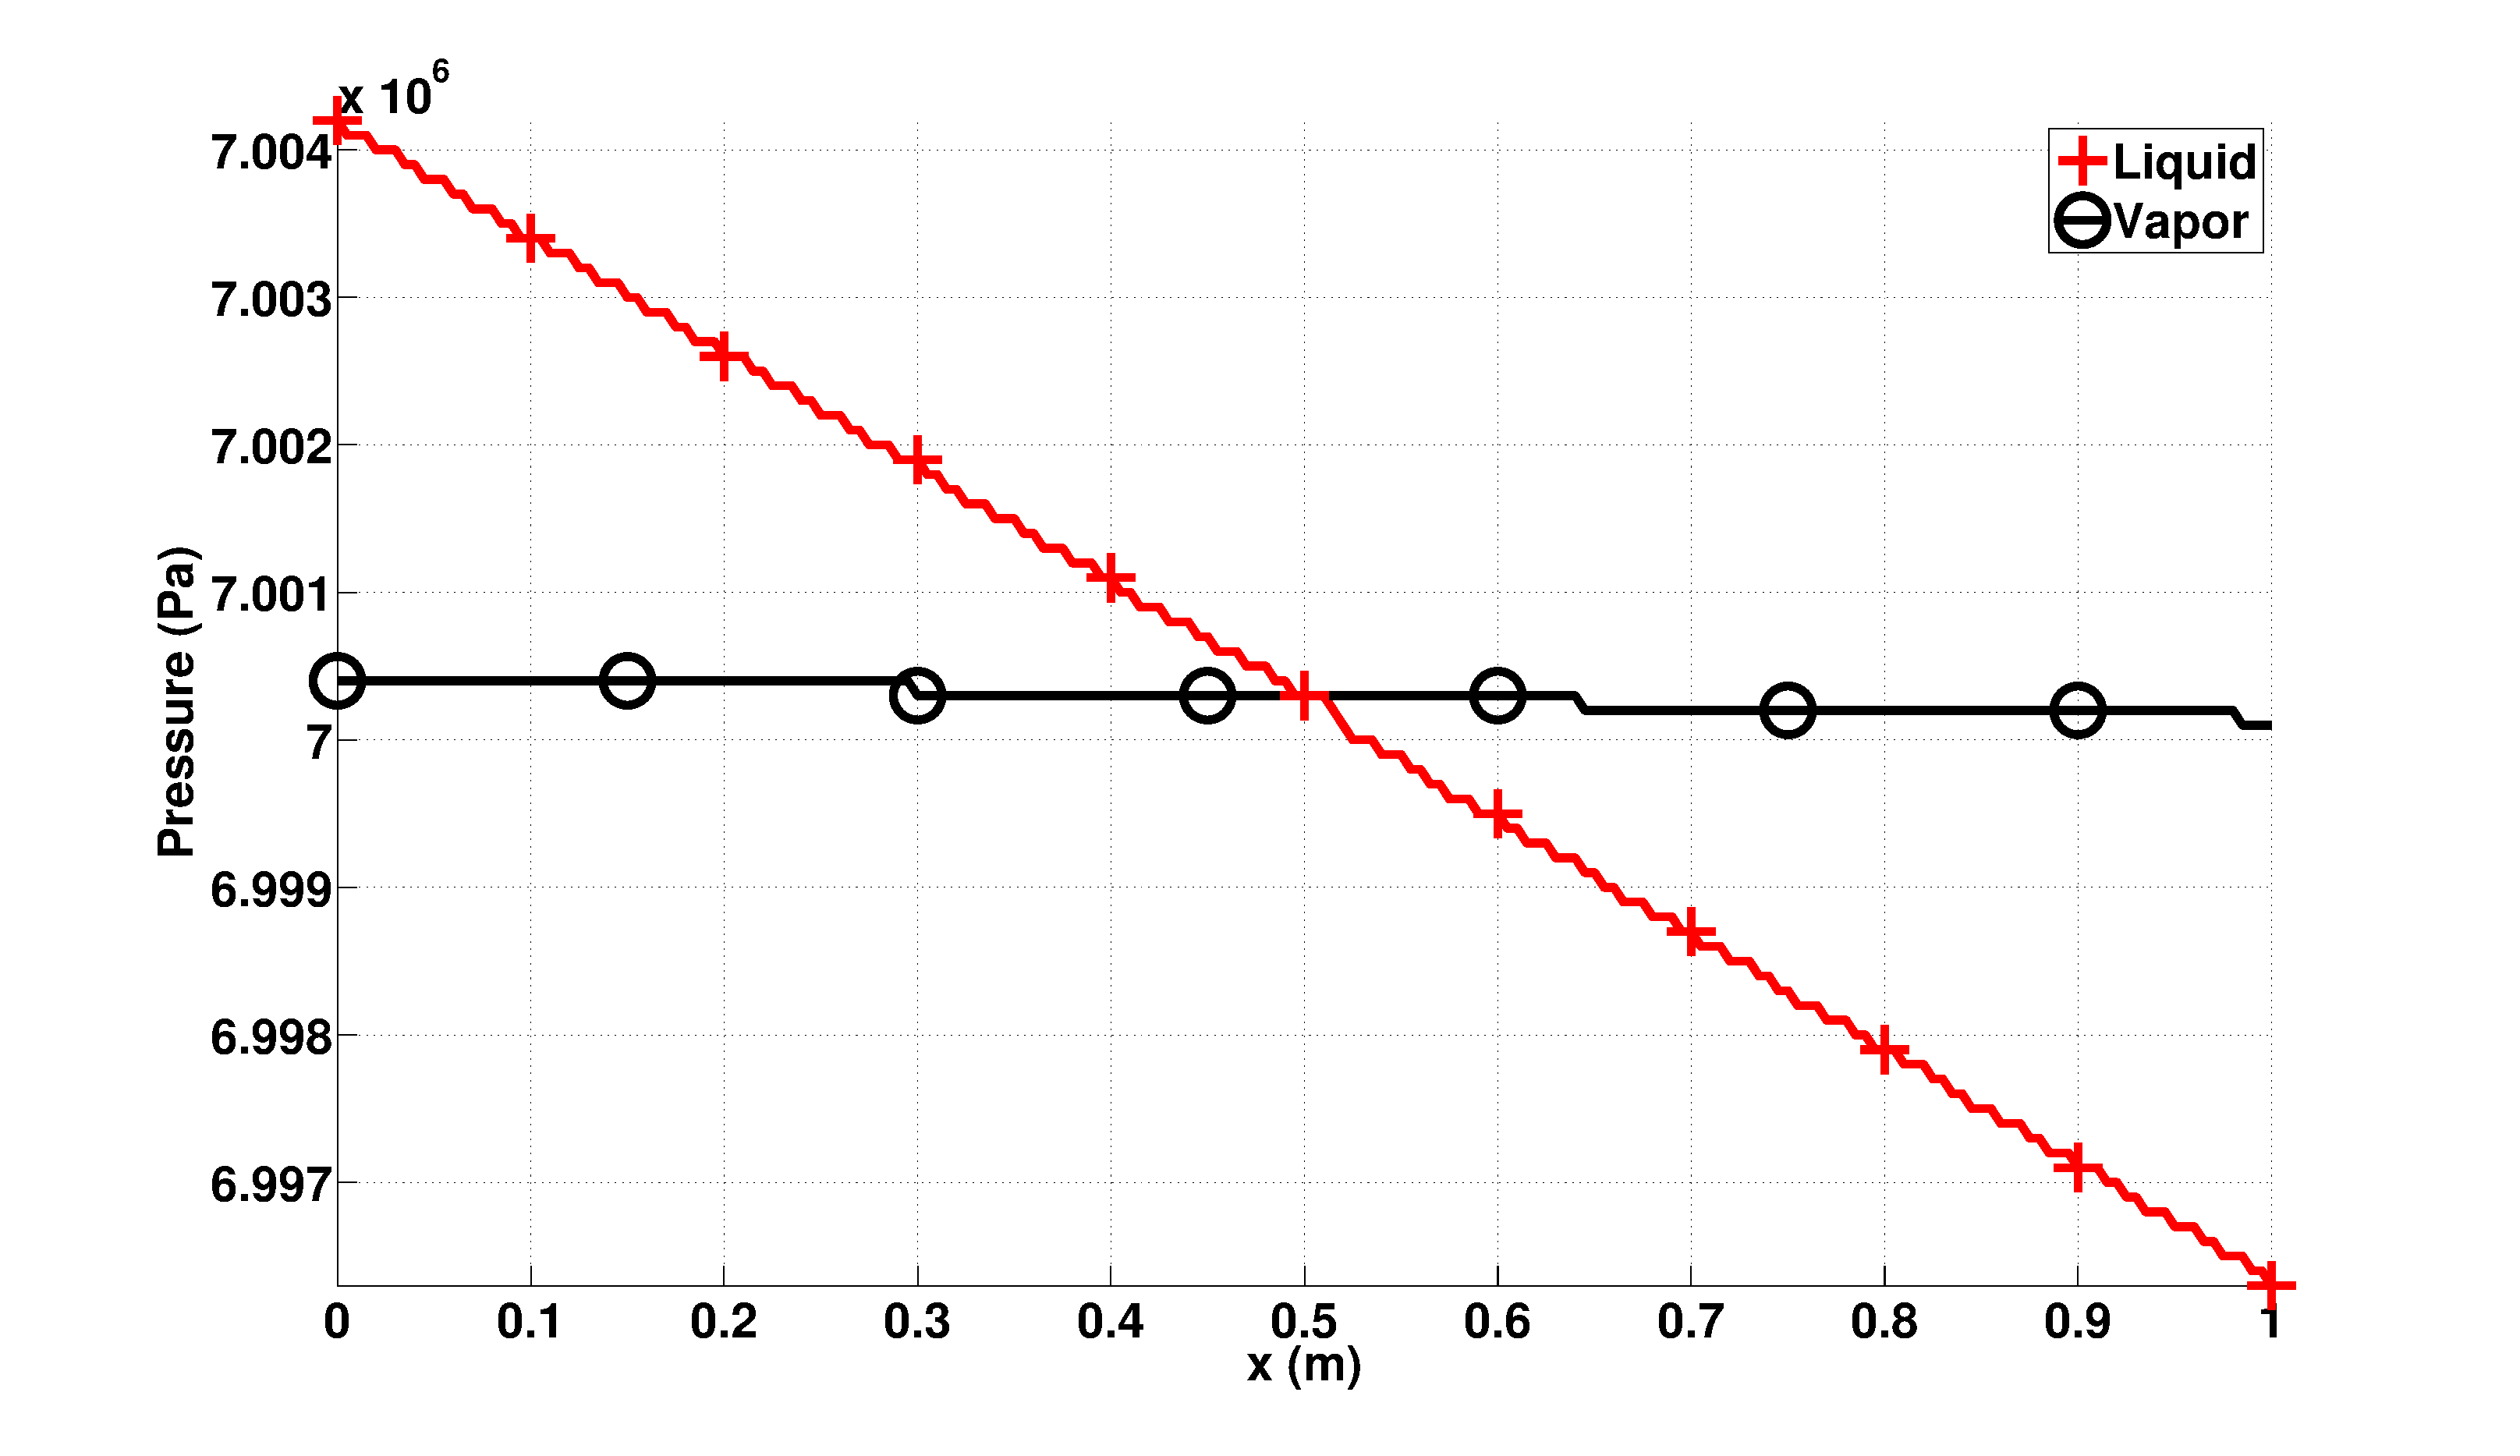
\includegraphics[width=\textwidth]{figures/hydrostatic-_two_phases_pressure.eps}
                \caption{Pressure}
                \label{fig:hydrostatic--press}
        \end{subfigure}        
        \begin{subfigure}[b]{0.495\textwidth}
                \centering
                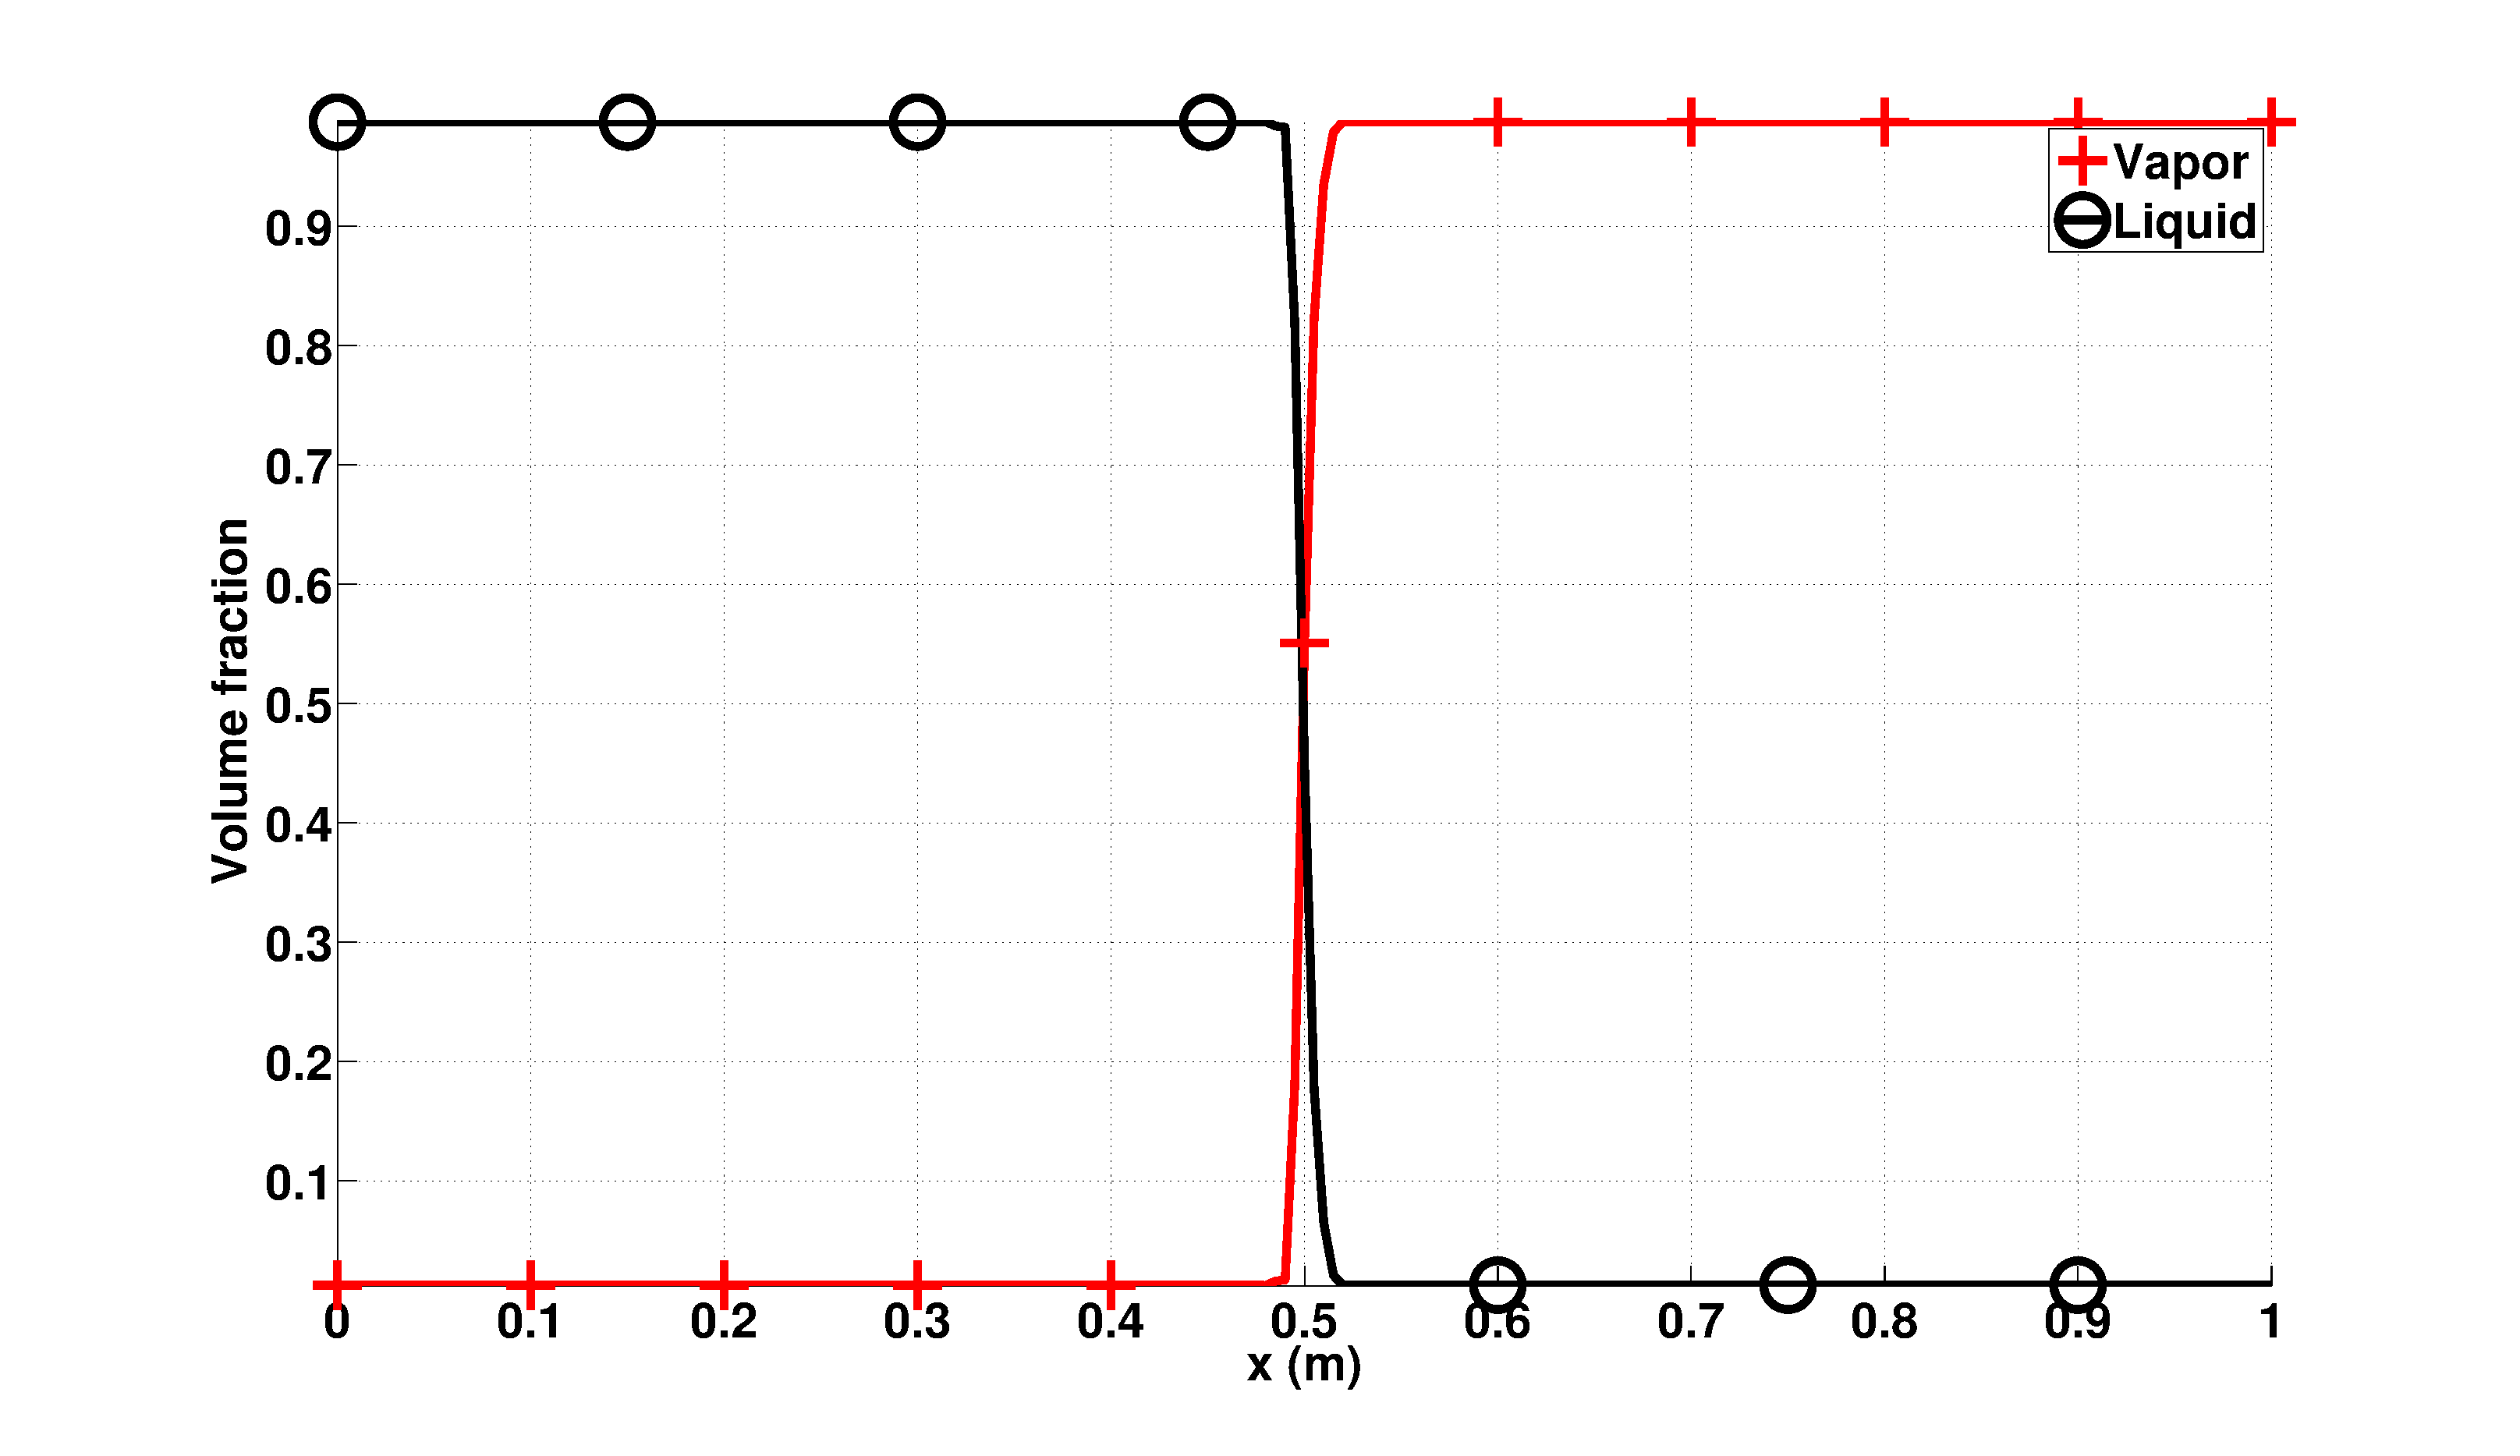
\includegraphics[width=\textwidth]{figures/hydrostatic-_two_phases_volume_fraction.eps}
                \caption{Volume fraction}
                \label{fig:hydrostatic--vf}
        \end{subfigure}
        \caption{Numerical solution of a two-phase flow with large relaxation coefficients at $t=305 \ \mu s$.}\label{fig:hydrostatic--variables}
\end{figure}
%
\begin{figure}[H]
        \centering
        \begin{subfigure}[b]{0.495\textwidth}
                \centering
                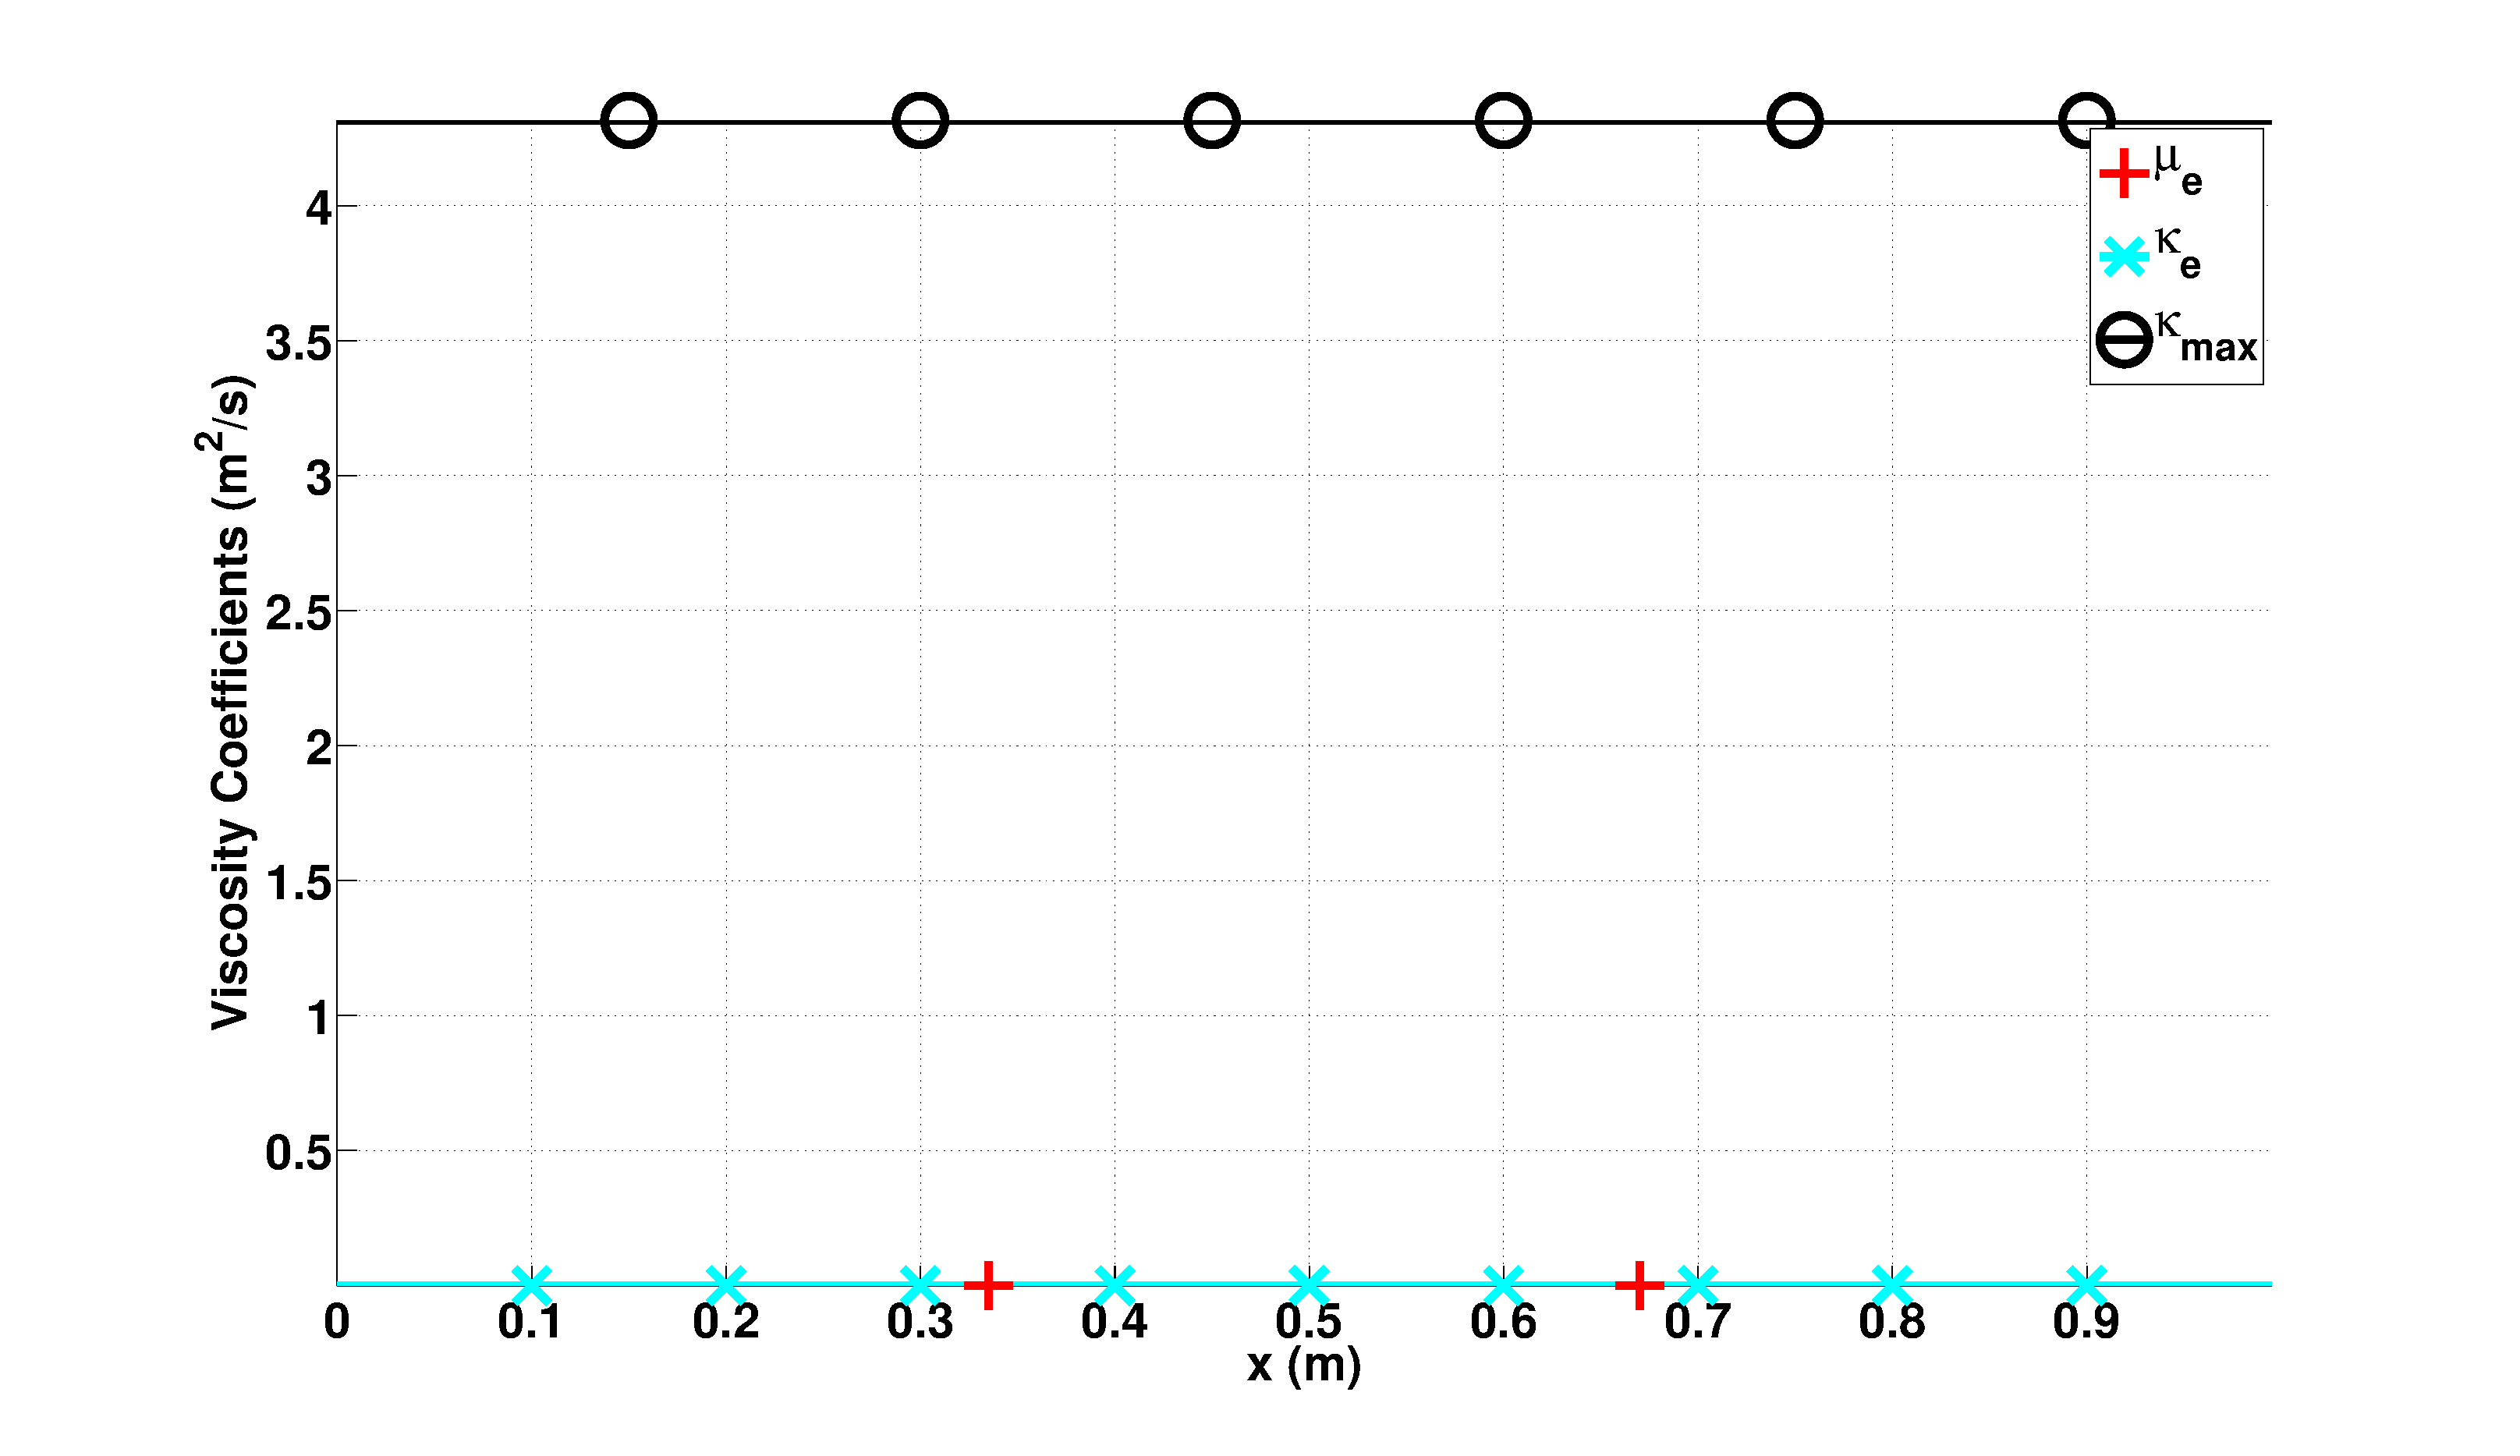
\includegraphics[width=\textwidth]{figures/hydrostatic-_liquid_viscosity_kappa_mu.eps}
                \caption{Viscosity coefficients for phase 1.}
                \label{fig:hydrostatic--visc-coeff-phase-1}
        \end{subfigure}%
        \begin{subfigure}[b]{0.495\textwidth}
                \centering
                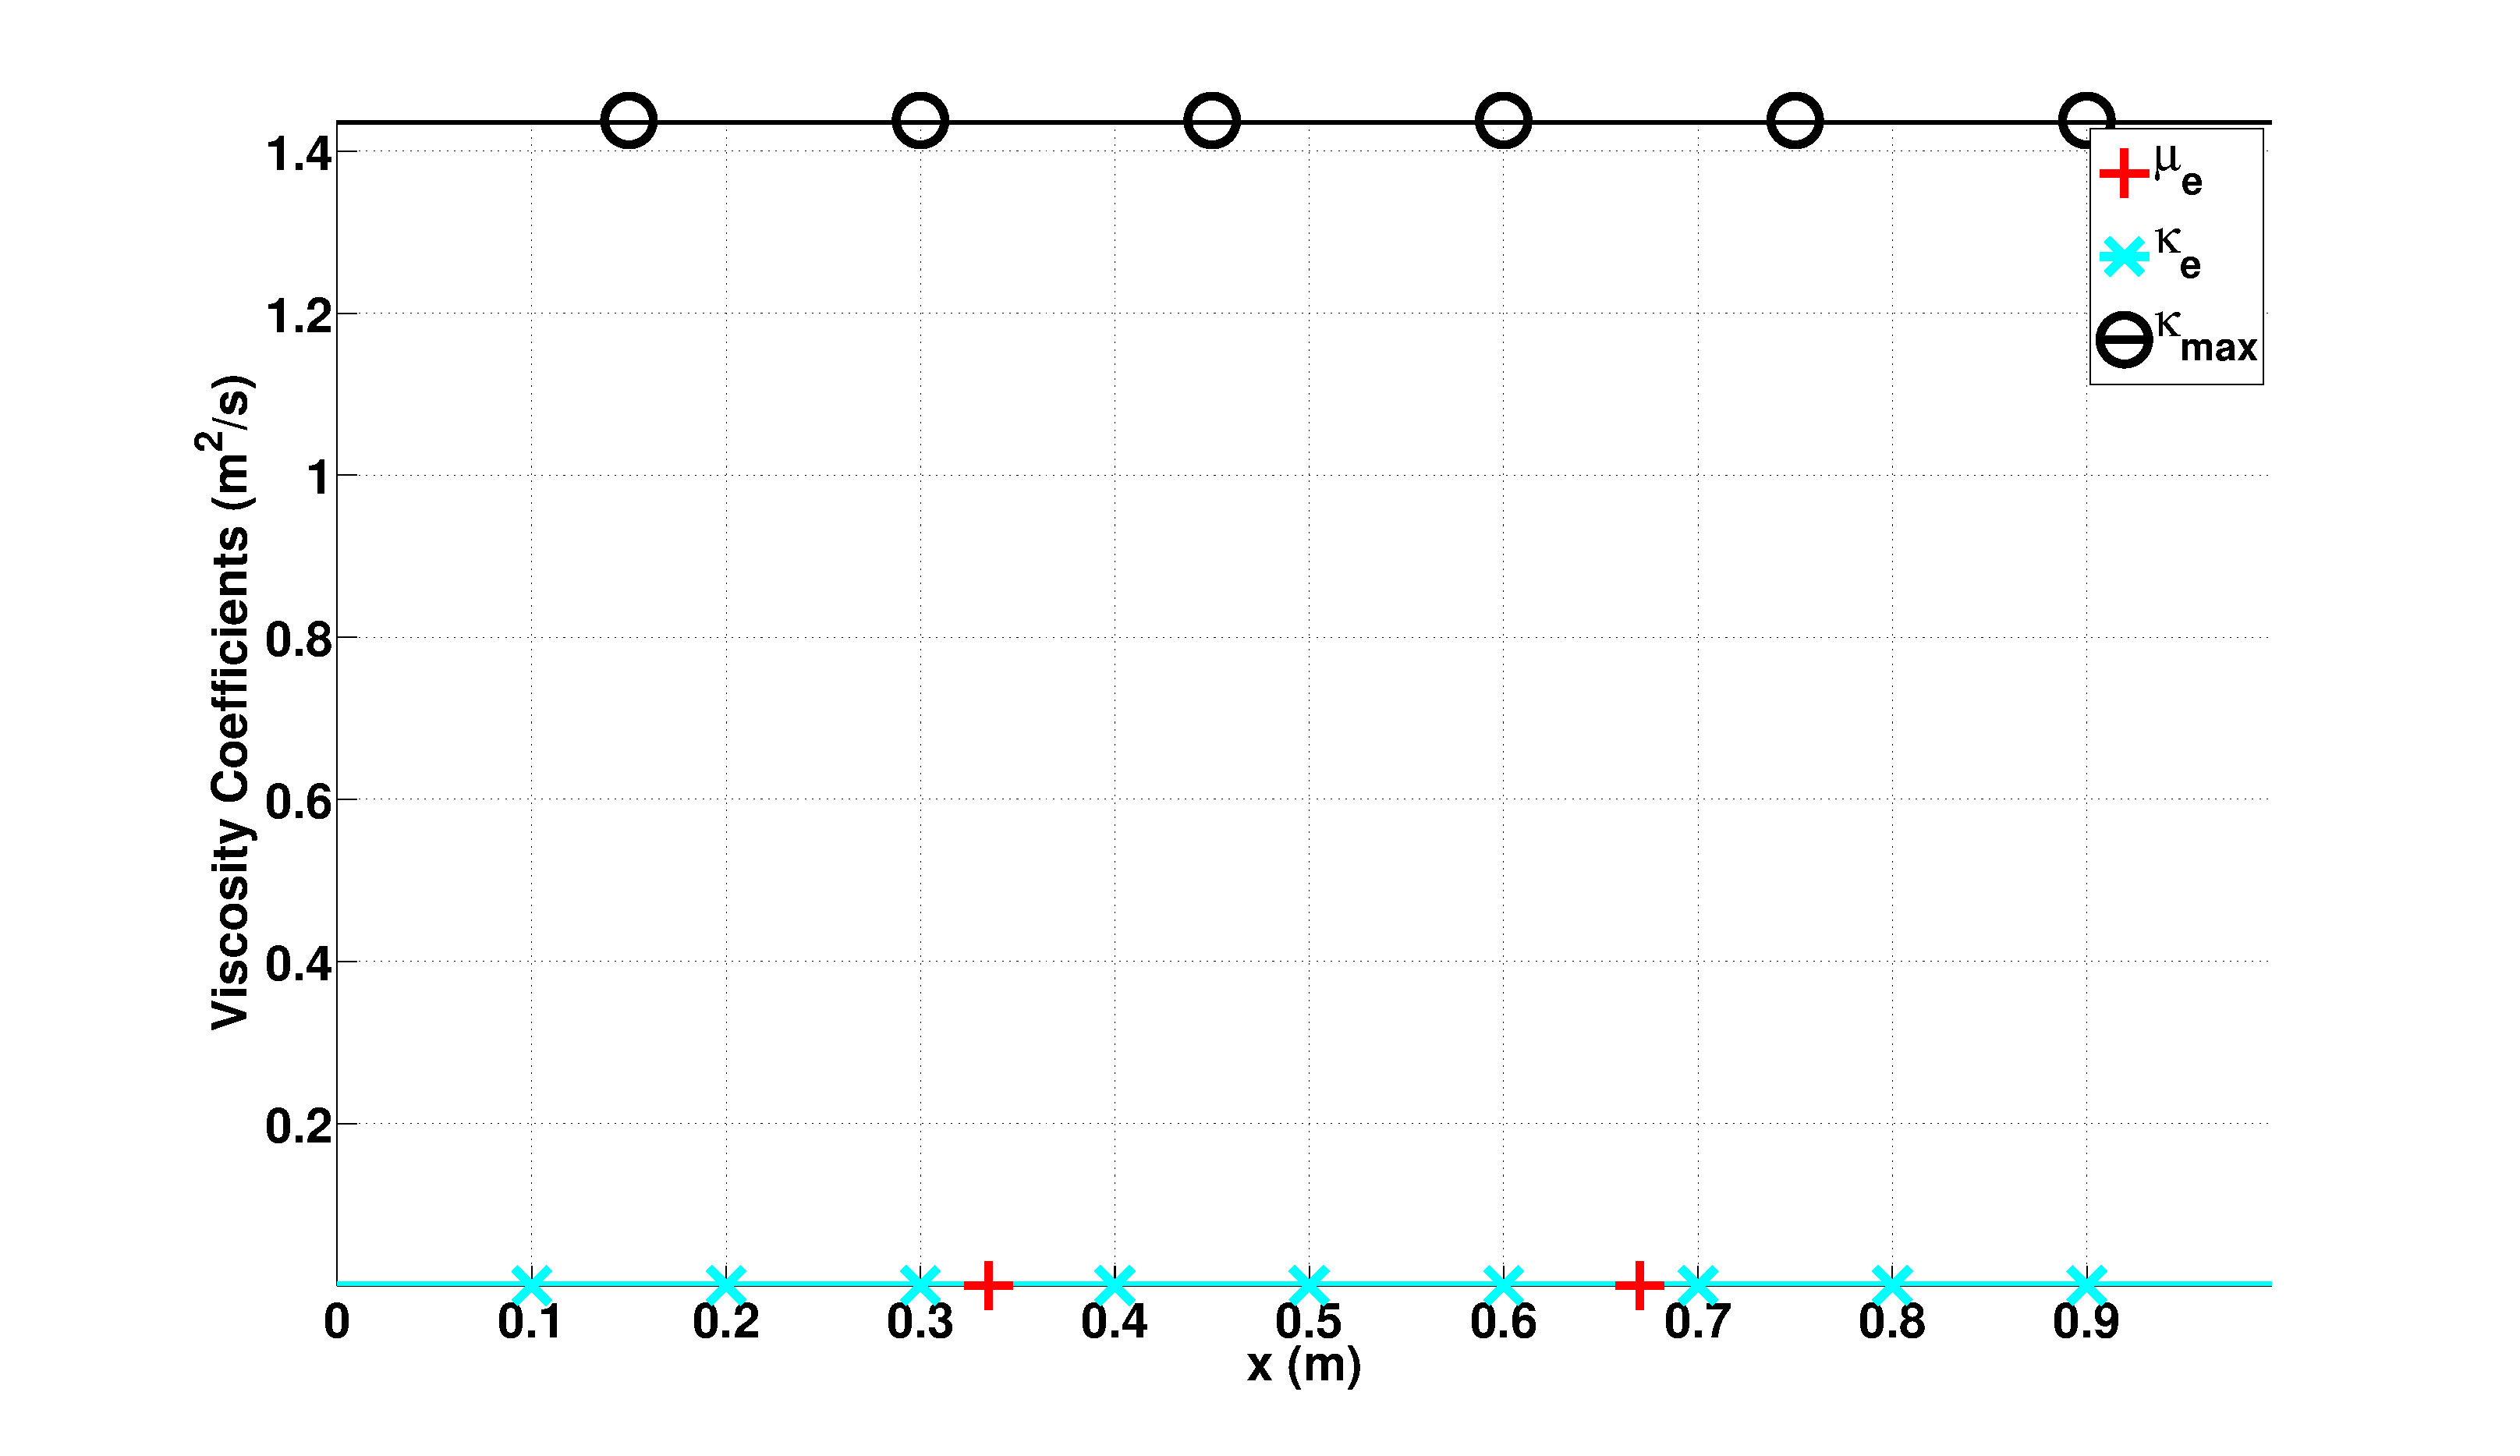
\includegraphics[width=\textwidth]{figures/hydrostatic-_vapor_viscosity_kappa_mu.eps}
                \caption{Viscosity coefficients for phase 2}
                \label{fig:hydrostatic--visc-coeff-phase-2}
        \end{subfigure}
        
        \begin{subfigure}[b]{0.495\textwidth}
                \centering
                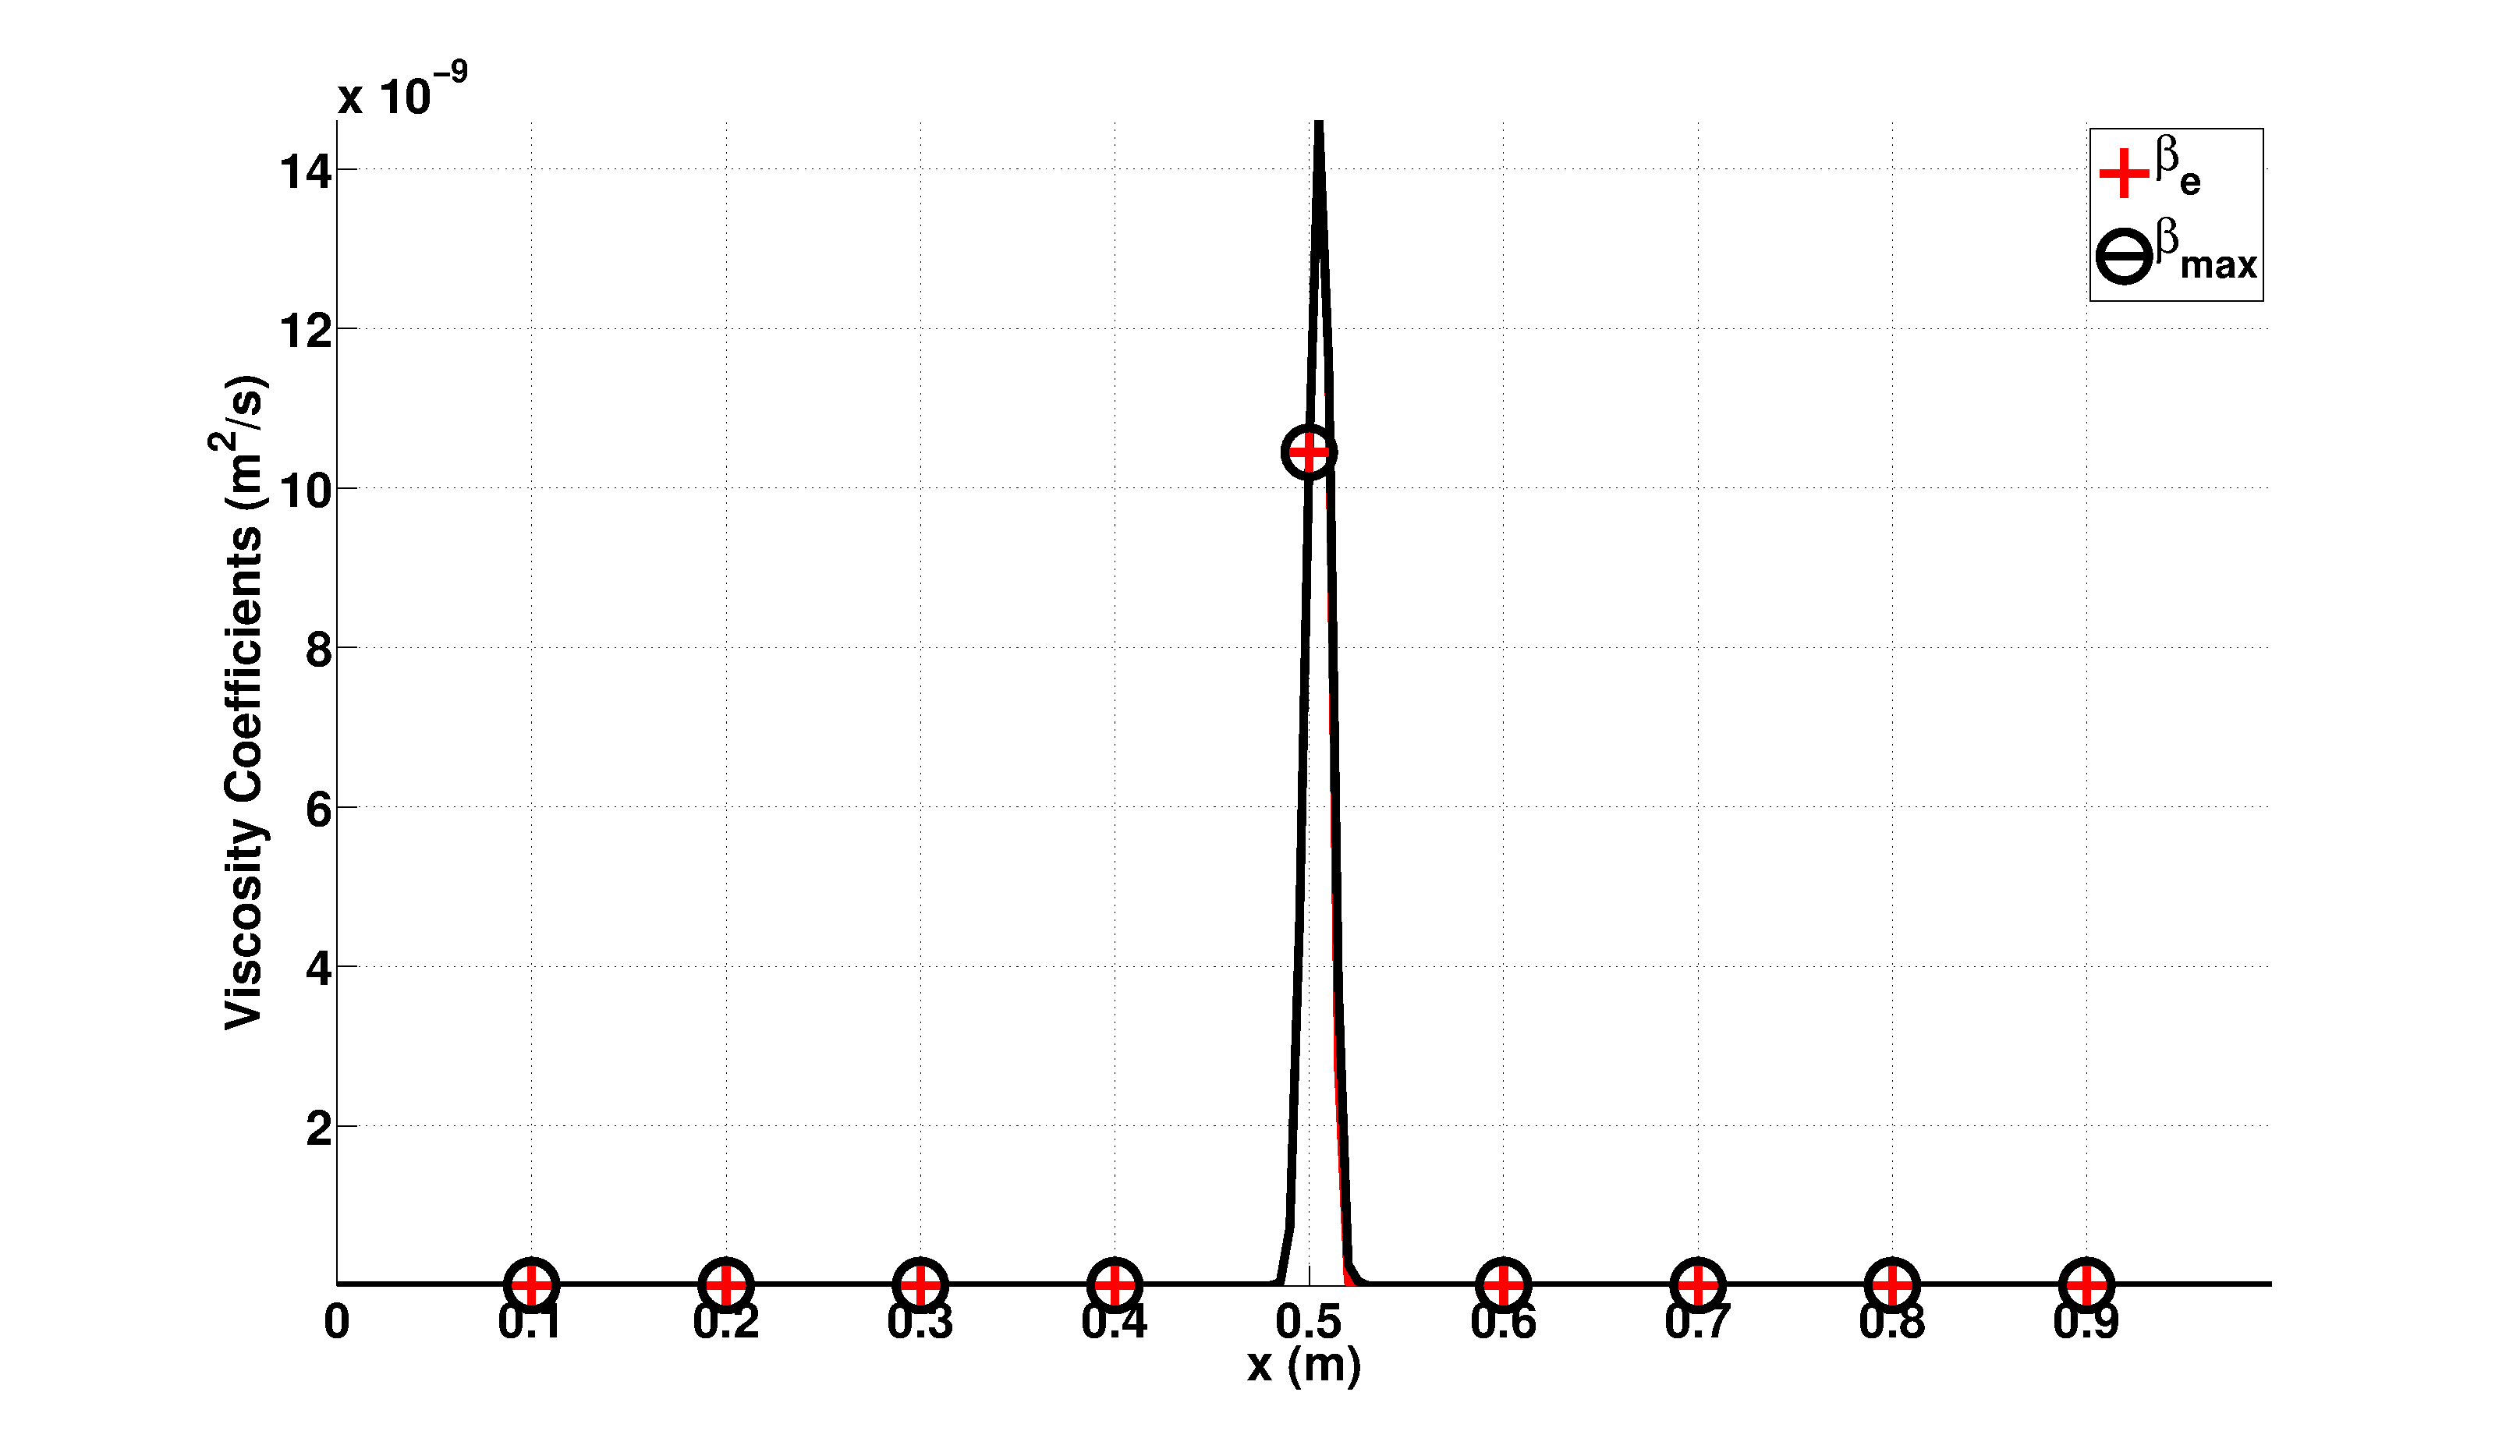
\includegraphics[width=\textwidth]{figures/hydrostatic-_liquid_beta.eps}
                \caption{Viscosity coefficients for the volume fraction equation of phase 1.}
                \label{fig:hydrostatic--beta}
        \end{subfigure}        
        \caption{Viscosity coefficients profiles for a two-phase flow with large relaxation coefficients at $t=305 \ \mu s$.}\label{fig:hydrostatic--visc-coeff}
\end{figure}
%
%
%%%%%%%%%%%%%%%%%%%%%%%%%%%%%%%%%%%%%
\subsection{Steady-state numerical solution of a Water Boiling Reactor (BWR)}\label{sec:bwr}
%%%%%%%%%%%%%%%%%%%%%%%%%%%%%%%%%%%%%
%
%%%%%%%%%%%%%%%%%%%%%%%%%%%%%%%%%%%%%%%%%%%%%%%%%%%%%%%%%%%%%%%%%%%%%%%%%%%%%
%%%%%%%%%%%%%%%%%%%%%%%%%%%%%%%%%%%%%%%%%%%%%%%%%%%%%%%%%%%%%%%%%%%%%%%%%%%%%
\section{Conclusions and future work}\label{sec:conclusion}
%%%%%%%%%%%%%%%%%%%%%%%%%%%%%%%%%%%%%%%%%%%%%%%%%%%%%%%%%%%%%%%%%%%%%%%%%%%%%
%%%%%%%%%%%%%%%%%%%%%%%%%%%%%%%%%%%%%%%%%%%%%%%%%%%%%%%%%%%%%%%%%%%%%%%%%%%%%
%
%We have derived a viscous regularization for the hyperbolic Seven-Equation two-phase flow Model. The regularization ensures positivity of the entropy residual, 
%uniqueness of the numerical solution for concave physical phasic entropy functions $s_k$, and is consistent with the viscous regularization derived for 
%Euler equations when one of the phases disappears. 
%We have also demonstrated that the proposed viscous regularization is compatible with the generalized Harten entropies that were initially derived for Euler equations. 
%
%The viscous regularization for the SEM equations involves a set of two positive viscosity coefficients for each phase, $\mu_k$ and $\kappa_k$, and one for the volume 
%fraction equation, $\beta_k$. The scaling of these viscosities is related to the numerical Reynolds and P\'eclet numbers, $\Re_k$, $\Pe_k^\mu$, and $\Pe_k^\kappa$. 
%Adequate scaling of these numbers has been devised for two important limit-cases: the low-Mach asymptotic limit and for non-isentropic flows. In the low-Mach regime, 
%we show that the incompressible equations are recovered when assuming that all of the non-dimensional numbers scale as one. The study of the non-isentropic case 
%shows that the scaling of the non-dimensionalized numbers is Mach-number dependent to ensure well-scaled dissipative terms in the vicinity of the shock.
%Based on these results, adequate scaling of the viscosities can be derived for all Mach numbers, as was the case for single-phase flows \cite{Marco_paper_low_mach}. 
%%
%We have also shown that the regularized SEM equations yields a regularized version of the five-equation flow model of Kapila by means of a Chapman-Enskog expansion.
%
%The ability of the proposed regularization to stabilize the SEM equations was numerically demonstrated using a shock tube problem, with the definitions of the 
%artificial viscosity coefficients borrowed from the local Lax-Friedrichs scheme. We have also analyzed the effect of removing stabilization from the volume fraction 
%and the continuity equations. The scaling effect of the viscous regularization on the numerical solution in the low-Mach asymptotic limit was numerically illustrated using a 1-D converging-diverging nozzle.
%
%As an extension of this work, the two-phase flow viscous regularization presented here should be utilized and tested with high-order, less dissipative, artificial viscosities, 
%such as the entropy viscosity (e.g., see \cite{jlg1} for single-phase supersonic flows and \cite{Marco_paper_low_mach} for single-phase subsonic and transonic flows). 
%We also note that the proposed regularization can also be employed using definitions of viscosity coefficients traditionally used in single-phase flows, e.g., 
%the Lapidus viscosity \cite{Lapidus_paper,Lapidus_book} and pressure-based viscosity, for two-phase flows \cite{PBV_book}. We intend on reporting on these findings in 
%a subsequent publication.
%
A version of the entropy viscosity method that is valid for a wide range of Mach numbers has been derived 
and presented for the inviscid two-phase flow Seven-Equation model.
The definition of the viscosity coefficients
is now consistent with the low-Mach asymptotic limit, does not require an analytical expression 
for the entropy function, and is therefore applicable to a larger variety of flow regimes, from very 
low-Mach flows to supersonic flows.
The method can also be used with the two-phase flow Seven-Equation model with variable area to solve nozzle flow problems.
It was demonstrated that the viscous regularization did not create any artificial waves when simulating independent two-phase flows.
Convergence of the numerical solution to the exact solution was demonstrated by computing the convergence rates of the L$_1$ and L$_2$ norms 
for $1$-D shock tube flows in straight pipes. The method was tested on various $1$-D tests obtained with Moose-based applications including a in-house code and the system code RELAP-7. The numerical method is capable of handling engineering tests such as hydrostatic pressure and water-hammer tests.
%For smooth solutions, second-order 
%convergence was verified; solutions with shocks converged with the expected theoretical rates of 1 (L$_1$-norm)
%and 1/2 (L$_2$-norm).

%The effectiveness of the method was also demonstrated in 2-D using a series of benchmark problems
%for both subsonic and supersonic flows in various geometries, with Mach numbers ranging from $10^{-7}$ to 
%2.5. For very low-Mach flows, we numerically verified that the steady-state pressure variations were proportional to 
%the square of the Mach number, as expected in the incompressible limit. A convergence study was carried out for a
%2D supersonic compression corner test case and rates of convergence of 1 (L$_1$-norm) and 1/2 (L$_2$-norm) were observed.

In the future, we plan to further apply the entropy viscosity method 
to the multi-dimensional Seven-Equation two-phase flow Model \cite{SEM}. 
%
%%%%%%%%%%%%%%%%%%%%%%%%%%%%%%%%%%%%%%%%%%%%%%%%%%%%%%%%%%%%%%%%%%%%%%%%%%%%%
%%%%%%%%%%%%%%%%%%%%%%%%%%%%%%%%%%%%%%%%%%%%%%%%%%%%%%%%%%%%%%%%%%%%%%%%%%%%%
\bibliography{mybibfile}
\end{document}